\documentclass[a4paper,11pt]{article}
\pdfoutput=1 % if your are submitting a pdflatex (i.e. if you have
             % images in pdf, png or jpg format)

\usepackage{jheppub} % for details on the use of the package, please
                     % see the JHEP-author-manual
\usepackage{enumerate}
\usepackage{feynmp}
\usepackage[T1]{fontenc} % if needed
\usepackage{lineno}
\usepackage{amsmath}
\usepackage{pdfpages}
\usepackage{pifont}% http://ctan.org/pkg/pifont
\usepackage{tikz}
\usepackage[compat=1.1.0]{tikz-feynman}
\newcommand{\cmark}{\ding{51}}%
\newcommand{\xmark}{\ding{55}}%
\newcommand{\Lecture}[1]
           {
             {\Huge\bf\underline{Week #1}}
           }
\usepackage{mathtools}
\usepackage{arev}
\usepackage{cancel}
%%% fixes the line numbering near \begin{align}
\newcommand*\patchAmsMathEnvironmentForLineno[1]{%
  \expandafter\let\csname old#1\expandafter\endcsname\csname #1\endcsname
  \expandafter\let\csname oldend#1\expandafter\endcsname\csname end#1\endcsname
  \renewenvironment{#1}%
     {\linenomath\csname old#1\endcsname}%
     {\csname oldend#1\endcsname\endlinenomath}}% 
\newcommand*\patchBothAmsMathEnvironmentsForLineno[1]{%
  \patchAmsMathEnvironmentForLineno{#1}%
  \patchAmsMathEnvironmentForLineno{#1*}}%
\AtBeginDocument{%
\patchBothAmsMathEnvironmentsForLineno{equation}%
\patchBothAmsMathEnvironmentsForLineno{align}%
\patchBothAmsMathEnvironmentsForLineno{flalign}%
\patchBothAmsMathEnvironmentsForLineno{alignat}%
\patchBothAmsMathEnvironmentsForLineno{gather}%
\patchBothAmsMathEnvironmentsForLineno{multline}%
}
%%
%% paragraphs with vertical space, no indent:
\parindent=0em \addtolength{\parskip}{2ex}
%%

\newcommand{\hideAnswers}{0}


\usepackage{slashed}
%%% exercise boxes:
\newcounter{exc}
\setcounter{exc}{0}
\newcommand{\exercise}[1]{\stepcounter{exc}\fbox{\parbox{0.985\hsize}{{\bf Exercise \arabic{exc}.} #1}}}
\newcommand{\inlineAnswer}[1]{\rotatebox{180}{\parbox{0.9\textwidth}{#1}}}
%%%%%%%%%%%%%%%%%%%%%%%%%%%%%%%%%%%%
%% things to do with "empty boxes"
%% that the students were suppose
%% to fill in - probably won't do that
%% here, but leave in for now to get 
%% the latex to compile.
%%
\usepackage{ifthen}

%\ifthenelse{\hideAnswers = 1}{%
%\newcommand{\answerbox}[1]{}%
%}{%
%\newcommand{\answerbox}[1]{\mbox{}\\{{\color{blue}\it\mbox{}#1}\color{black}}}%
%}

\newcommand{\answerbox}[1]{
\ifthenelse{\hideAnswers = 1}{%
}{%
{\mbox{}\\{{\color{blue}\it\mbox{}#1}\color{black}}}%
}}

\newcommand{\hide}{0}
\newcommand{\teach}{1}

\ifthenelse{\hide = 1}{
 \newcommand{\emptyeq}[2]{\fbox{\parbox{0.98\hsize}{\mbox{}\vspace{#1}\\\begin{equation}\end{equation}}}}
 \newcommand{\emptyeqlab}[3]{\fbox{\parbox{0.98\hsize}{\mbox{}\vspace{#1}\\\begin{equation}\label{#2}\end{equation}}}}
 \newcommand{\emptybox}[1]{\fbox{\parbox{\textwidth}{\mbox{}\vspace{#1}\\\mbox{}}}}
 \newcommand{\emptyfig}[2]{\fbox{\parbox{0.98\hsize}{\mbox{}\vspace{#1}\\\begin{figure}\end{figure}}}}
 \newcommand{\emptyfiglab}[3]{\fbox{\parbox{0.98\hsize}{\mbox{}\vspace{#1}\\\begin{figure}\label{#2}\end{figure}}}}
}{
 \ifthenelse{\teach = 1}{
 \newcommand{\emptyeq}[2]{\fbox{\parbox{0.98\hsize}{\parbox[t]{0.95\textwidth}{#2}\vspace{#1}\mbox{}\\\mbox{ }}}}
 \newcommand{\emptyeqlab}[3]{\fbox{\parbox{0.98\hsize}{\parbox[t]{0.95\textwidth}{#3}\vspace{#1}\mbox{}\\\mbox{ }}}}
% \newcommand{\emptyeqlab}[3]{\fbox{\parbox{0.98\hsize}{\parbox{0ex}{\mbox{}\vspace{#1}\\\mbox{}}#3}}}
 \newcommand{\emptybox}[1]{\fbox{\parbox{\textwidth}{\mbox{}\vspace{#1}\\\mbox{}}}}
 \newcommand{\emptyfig}[2]{\fbox{\parbox{0.98\hsize}{\parbox{0ex}{\mbox{}\vspace{#1}\\\mbox{}} #2}}}
 \newcommand{\emptyfiglab}[3]{\fbox{\parbox{0.98\hsize}{\parbox{0ex}{\mbox{}\vspace{#1}\\\mbox{}}#3}}}
 }{
 \newcommand{\emptybox}[1]{\fbox{\parbox{\textwidth}{\mbox{}\vspace{#1}\\\mbox{}}}}
 \newcommand{\emptyeq}[2]{#2}
 \newcommand{\emptyeqlab}[3]{#3}
 \newcommand{\emptyfig}[2]{#2}
 \newcommand{\emptyfiglab}[3]{#3}
 }
}

%%%%%%%%%%%%%%%%%%%%%%%%%%%%%%%%%%%%
%% some not so mathematical commands.
\newcommand{\figref}[1]{Figure~\ref{#1}}
\newcommand{\Figref}[1]{Figure~\ref{#1}}
\newcommand{\tabref}[1]{Table~\ref{#1}}
\newcommand{\Tabref}[1]{Table~\ref{#1}}
\newcommand{\secref}[1]{section~\ref{#1}}
\newcommand{\Secref}[1]{Section~\ref{#1}}
\newcommand{\appref}[1]{appendix~\ref{#1}}
\newcommand{\Appref}[1]{Appendix~\ref{#1}}
\newcommand{\eqnref}[1]{equation~\ref{#1}}
\newcommand{\Eqnref}[1]{Equation~\ref{#1}}

\newcommand{\st}{\ensuremath{\mbox{}^{\mathrm{st}}}}
\newcommand{\nd}{\ensuremath{\mbox{}^{\mathrm{nd}}}}
\newcommand{\rd}{\ensuremath{\mbox{}^{\mathrm{rd}}}}
\newcommand{\te}{\ensuremath{\mbox{}^{\mathrm{th}}}}

\newcommand{\cs}{\ensuremath{\mathcal{C}}}
\newcommand{\ps}{\ensuremath{\mathcal{P}}}
\newcommand{\ts}{\ensuremath{\mathcal{T}}}
\newcommand{\cp}{\ensuremath{\mathcal{CP}}}
\newcommand{\cpt}{\ensuremath{\mathcal{CPT}}}
\newcommand{\cpv}{\cp\ violation}
\newcommand{\sm}{Standard Model}
\newcommand{\Se}{Schr\"odinger Equation}

\newcommand{\topar}{\ensuremath{\stackrel{\ps}{\longrightarrow}}}

\newcommand{\httplink}[1]{\href{#1}{\texttt{#1}}}
\newcommand{\httplinkUscore}[2]{\href{#1}{\texttt{#2}}}
\newcommand{\hepArchive}[1]{\href{http://arXiv.org/abs/#1}{[arXiv:{#1}]}}
\newcommand{\hepArchiveURL}[1]{\hepArchive{#1} {\small\httplink{http://arXiv.org
/abs/#1}}}
%%%%%%%%%%%%%%%%%%%%%%%%%%%%%%%%%%%%

\newcommand{\Imag}{\ensuremath{\mathsf{Im}}}
\newcommand{\Real}{\ensuremath{\mathsf{Re}}}
%\newcommand{\mod}[1]{\ensuremath{\left|#1\right|}}
\newcommand{\deff}{\stackrel{\mathrm{def}}{=}}
\newcommand{\perc}{\%}
\newcommand{\Lik}{\ensuremath{\mathcal{L}}}
\newcommand{\logLik}{\ensuremath{\ln\!\left(\Lik\right)}}
\newcommand{\dbyd}[2]{\ensuremath{\frac{\mathrm{d}#1}{\mathrm{d}#2}}}
\newcommand{\partdbyd}[2]{\ensuremath{\frac{\mathsf{\partial}#1}{\mathsf{\partial}#2}}}

\newcommand{\contrafo}[2]{\partdbyd{x^{\prime #1}}{x^{#2}}}
\newcommand{\covtrafo}[2]{\partdbyd{x^{#1}}{x^{\prime #2}}}
\newcommand{\DS}{\displaystyle}

\newcommand{\dx}[1]{\ensuremath{\mathrm{d}\:\!\!#1}}
\newcommand{\dIII}[1]{\ensuremath{\mathrm{d^3}\:\!\!#1}}
\newcommand{\dIV}[1]{\ensuremath{\mathrm{d^4}\:\!\!#1}}
\newcommand{\bra}[1]{\ensuremath{ \langle #1 |}}
\newcommand{\ket}[1]{\ensuremath{ | #1 \rangle}}
\newcommand{\braket}[2]{\ensuremath{ \left< #1\; |\; #2 \right>}}
%\newcommand{\mod}[1]{\ensuremath{\left| #1 \right|}}

\newcommand{\vII}[2]{\ensuremath{%
  \left( \begin{array}{c} #1 \\ #2 \end{array} \right)}}
\newcommand{\vIInb}[2]{\ensuremath{%
  \begin{array}{c} #1 \\ #2 \end{array}}}
\newcommand{\vIII}[3]{\ensuremath{%
  \left( \begin{array}{c} #1 \\ #2 \\ #3\end{array} \right)}}
\newcommand{\vIV}[4]{\ensuremath{%
  \left( \begin{array}{c} #1 \\ #2 \\ #3 \\ #4\end{array} \right)}}

\newcommand{\rowII}[2]{\ensuremath{%
  \left( #1\;\; #2 \right)}}
\newcommand{\rowIII}[3]{\ensuremath{%
  \left( #1\;\; #2 \;\; #3 \right)}}
\newcommand{\rowIV}[4]{\ensuremath{%
  \left( #1\;\; #2 \;\; #3\;\; #4 \right)}}

\newcommand{\mII}[4]{\ensuremath{%
  \left( \begin{array}{cc} #1 & #2 \\ #3 & #4 \end{array} \right)}}
\newcommand{\mIII}[9]{\ensuremath{%
  \left( \begin{array}{ccc} #1 & #2 & #3 \\ 
                           #4 & #5 & #6 \\
                           #7 & #8 & #9 \end{array} \right)}}
                           
                         
\newcommand{\mDiagIII}[3]{\ensuremath{%
  \left( \begin{array}{ccc} #1 &    &    \\ 
                               & #2 &    \\
                               &    & #3 \end{array} \right)}}
\newcommand{\mDiagIV}[4]{\ensuremath{%
  \left( \begin{array}{cccc}  #1 &     &     &     \\ 
                                 &  #2 &     &     \\
                                 &     &  #3 &     \\
                                 &     &     & #4 \end{array} \right)}}

\newcommand{\PauliSpinI}{\mII{0}{1}{1}{0}}
\newcommand{\PauliSpinII}{\mII{0}{-i}{i}{0}}
\newcommand{\PauliSpinIII}{\mII{1}{0}{0}{-1}}

\newcommand{\op}[1]{\ensuremath{\mathbf{#1}}}
\newcommand{\leish}{\ensuremath{\stackrel{\textstyle{<}}{\sim}}}
\newcommand{\geish}{\ensuremath{\stackrel{\textsyyle{>}}{\sim}}}
\newcommand{\half}{\ensuremath{\frac{1}{2}}}
\newcommand{\third}{\ensuremath{\frac{1}{3}}}
\newcommand{\quarter}{\ensuremath{\frac{1}{4}}}
\newcommand{\sqrtHalf}{\ensuremath{\frac{1}{\sqrt{2}}}}
\newcommand{\Del}{\ensuremath{\Delta\!}}
%\newcommand{\diracsl}[1]{\ensuremath{#1\!\!\!\!\!\!\!\mbox{\hspace{0.1em}\large$\not$}\;\;\;}}
\newcommand{\diracsl}[1]{\ensuremath{\slashed{#1}}}
%%\newcommand{\inlinediracsl}[1]{\ensuremath{#1\!\!\!\!\!\mbox{\hspace{0.1em}\large$\not$}\;\;\:}}
\newcommand{\inlinediracsl}[1]{\ensuremath{\slashed{#1}}}
\newcommand{\partslash}{\diracsl{\partial}}
\newcommand{\pslash}{\diracsl{p}}
\newcommand{\order}[1]{\ensuremath{\mathcal{O}\!\left(#1\right)}}
\newcommand{\Efield}{\ensuremath{\vec{\mathcal{E}}}}
\newcommand{\Bfield}{\ensuremath{\vec{\mathcal{B}}}}
\newcommand{\nablaVec}{
\ensuremath{\vIII{\frac{\partial}{\partial x}}{\frac{\partial}{\partial y}}{\frac{\partial}{\partial z}}
 }}
\newcommand{\gradnabla}{\ensuremath{\vec{\nabla}}}
\newcommand{\divnabla}{\ensuremath{\vec{\nabla}\cdot }}
\newcommand{\curlnabla}{\ensuremath{\vec{\nabla}\times }}
\newcommand{\rotnabla}{\curlnabla}
\newcommand{\continuity}[2]{\frac{\partial #1}{\partial t} +
                                 \divnabla\vec{#2} = 0}
\newcommand{\unitMatrix}{\ensuremath{1\!\!\!1}}
\newcommand{\pderiv}[1]{\ensuremath{\frac{\partial }{\partial #1}}}
\newcommand{\pderivOf}[2]{\ensuremath{\frac{\partial #1}{\partial #2}}}
\newcommand{\gradIII}[1]{
\ensuremath{
\vIII{\pderivOf{#1}{x}}{\pderivOf{#1}{y}}{\pderivOf{#1}{z}}
}
}
\newcommand{\curlIII}[3]{
\ensuremath{
\vIII{%
\pderivOf{#3}{y} - \pderivOf{#2}{z}}{%
- \pderivOf{#3}{x} + \pderivOf{#1}{z}}{%
\pderivOf{#2}{x} - \pderivOf{#1}{y}}%
}
}
\newcommand{\divOf}[3]{\ensuremath{
\pderivOf{#1}{x} + \pderivOf{#2}{y} + \pderivOf{#3}{z}}}
\newcommand{\sel}[1]{\ensuremath{\stackrel{\downarrow}{#1}}}
\newcommand{\curl}{\ensuremath{\mathrm{curl}}}
\renewcommand{\div}{\ensuremath{\mathrm{div}}}
\newcommand{\grad}{\ensuremath{\mathrm{grad}}}
%%
\newcommand{\dcovmu}{\ensuremath{\partial_{\mu}}}
\newcommand{\dconmu}{\ensuremath{\partial^{\mu}}}
\newcommand{\dcovnu}{\ensuremath{\partial_{\nu}}}
\newcommand{\dconnu}{\ensuremath{\partial^{\nu}}}

\newcommand{\ME}{\ensuremath{\mathcal{M}}}
\newcommand{\Msq}{\ensuremath{\left|\ME\right|^2}}
\newcommand{\AvMsq}{\expect{\Msq}}
%%
\newcommand{\JxMIII}{\ensuremath{
    \left(\begin{array}{ccc}
        0 &   0     &     0     \\
        0 &   0     &     -i  \\
        0 &   i     &     0  \\
      \end{array}\right)}}
\newcommand{\JyMIII}{\ensuremath{
    \left(\begin{array}{ccc}
        0    & 0 &  i  \\
        0    & 0 &  0 \\
        -i    & 0 &  0  \\
      \end{array}\right)}}
\newcommand{\JzMIII}{\ensuremath{
    \left(\begin{array}{ccc}
        0     &  -i        & 0 \\
        i     &   0        & 0 \\
        0     &   0        & 0 \\
      \end{array}\right)}}

%%
\newcommand{\PauliX}{\ensuremath{
    \mII{0}{1}{1}{0}
}}
\newcommand{\PauliY}{\ensuremath{
    \mII{0}{-i}{i}{0}
}}
\newcommand{\PauliZ}{\ensuremath{
    \mII{1}{0}{0}{-1}
}}
\newcommand{\RotIIIX}[1]{\ensuremath{
   \mIII{1}{0}{0}
        {0}{\cos(#1)}{\sin(#1)}
        {0}{-\sin(#1)}{\cos(#1)}
}}
\newcommand{\RotIIIY}[1]{\ensuremath{
   \mIII{\cos(#1)}{0}{-\sin(#1)}
        {\sin(#1)}{0}{\cos(#1)}
        {0}{1}{0}
}}
\newcommand{\RotIIIZ}[1]{\ensuremath{
   \mIII{\cos(#1)}{\sin(#1)}{0}
        {-\sin(#1)}{\cos(#1)}{0}
        {0}{0}{1}
}}

%
\newcommand{\expect}[1]{\ensuremath{\left\langle #1 \right\rangle}}
%

\newcommand{\xbyx}[2]{\ensuremath{\pderivOf{x^{#1}}{x^{#2}}}}
\newcommand{\xpbyxp}[2]{\ensuremath{\pderivOf{x^{\prime #1}}{x^{\prime #2}}}}
\newcommand{\covt}[2]{\ensuremath{\pderivOf{x^{#1}}{x^{\prime #2}}}}
\newcommand{\cont}[2]{\ensuremath{\pderivOf{x^{\prime #1}}{x^{ #2}}}}

\newcommand{\crossProduct}[6]{%
\ensuremath{%
\vIII{%
 #2 #6 - #3 #5}{
 -#1 #6 + #3 #4}{
 #1 #5 - #2 #4}
}
}

\newcommand{\EuLa}[2]{\ensuremath{%
  \frac{\partial #1}{\partial #2} -
  \frac{d}{dt}\frac{\partial #1}{\partial (\dot{#2})}
}}

\newcommand{\units}[1]{\ensuremath{\mathrm{#1}}}
\newcommand{\un}[2]{\ensuremath{#1\,\units{#2}}}


\newcommand{\m}{\units{m}}
\newcommand{\cm}{\units{cm}}
\newcommand{\mm}{\units{mm}}
\newcommand{\mum}{\units{\mu m}}
\newcommand{\sqmtr}{\ensuremath{\units{m}^2}}
\newcommand{\sqcm}{\ensuremath{\units{cm}^2}}
\newcommand{\sqmm}{\ensuremath{\units{mm}^2}}
\newcommand{\cubicm}{\ensuremath{\units{m}^3}}
\newcommand{\ccm}{\ensuremath{\units{cm}^3}}
\newcommand{\cmm}{\ensuremath{\units{mm}^3}}

\newcommand{\V}{\units{V}}
\newcommand{\kV}{\units{kV}}

\newcommand{\eV}{\units{eV}}
\newcommand{\keV}{\units{keV}}
\newcommand{\MeV}{\units{MeV}}
\newcommand{\GeV}{\units{GeV}}

\newcommand{\flux}{\units{cm^{-2}s^{-1}}}
\newcommand{\radlength}{\units{X_0}}

\newcommand{\degrees}[1]{\ensuremath{\mathrm{#1^{\circ}}}}
\newcommand{\centigrade}[1]{\ensuremath{\mathrm{#1^{\circ}C}}}

%% 
%% \newlength{\fntxvi} \newlength{\fntxvii}
%% \newcommand{\chem}[1]{
%%  {
%%  \fontencoding{OMS}\fontfamily{cmsy}\selectfont
%%  \fntxvi\the\fontdimen16\font
%%  \fntxvii\the\fontdimen17\font
%%  \fontdimen16\font=3pt\fontdimen17\font=3pt
%%  $\mathrm{#1}$
%%  \fontencoding{OMS}\fontfamily{cmys}\selectfont
%%  \fontdimen16\font=\fntxvi \fontdimen17\font=\fntxvii
%%  }
%% }

\newcommand{\chem}[1]{\ensuremath{\mathrm{#1}}}
\newcommand{\coord}[1]{\ensuremath{#1}}
\newcommand{\ten}[2]{\mbox{\ensuremath{#1\cdot 10^{#2}}}}
\newcommand{\E}[1]{\ensuremath{\cdot 10^{#1}}}


%
%-------------------------------------------------------------------
\newcommand{\prt}[1]{\ensuremath{{\rm #1}}}
\newcommand{\qrk}[1]{\ensuremath{#1}}
%-------------------------------------------------------------------
\newcommand{\Bo}{\prt{B^0}}
\newcommand{\Bob}{\prt{\overline{B}^0}}
\newcommand{\Bh}{\prt{B_{H}}}
\newcommand{\Bl}{\prt{B_{L}}}
\newcommand{\Bsh}{\prt{B_{sH}}}
\newcommand{\Bsl}{\prt{B_{sL}}}
\newcommand{\Bdh}{\prt{B_{dH}}}
\newcommand{\Bdl}{\prt{B_{dL}}}
\newcommand{\Bso}{\prt{B_{s}^0}}
\newcommand{\Bsob}{\prt{\overline{B_{s}^0}}}
\newcommand{\Bdo}{\prt{B_{d}^0}}
\newcommand{\Bdob}{\prt{\overline{B}_{d}^0}}
\newcommand{\Bp}{\prt{B^+}}
\newcommand{\Bm}{\prt{B^-}}
\newcommand{\Bpm}{\prt{B^{\pm}}}
\newcommand{\Bmp}{\prt{B^{\mp}}}
\newcommand{\Dst}{\prt{{D}^{\ast}}}
\newcommand{\Dstp}{\prt{{D}^{\ast +}}}
\newcommand{\Dstm}{\prt{{D}^{\ast -}}}
\newcommand{\aI}{\prt{a_1}}
\newcommand{\aIp}{\prt{a_1^+}}
\newcommand{\aIm}{\prt{a_1^-}}
\newcommand{\pion}{\prt{\pi}}
\newcommand{\pip}{\prt{\pi^+}}
\newcommand{\pim}{\prt{\pi^-}}
\newcommand{\piz}{\prt{\pi^0}}
\newcommand{\Do}{\prt{D^{0}}}
\newcommand{\Dob}{\prt{\overline{D}^0}}
\newcommand{\Ds}{\prt{D_s}}
\newcommand{\Dso}{\prt{D_s^{0}}}
\newcommand{\Dsob}{\prt{\overline{D}_s^0}}
\newcommand{\Kp}{\prt{K^+}}
\newcommand{\Km}{\prt{K^-}}
\newcommand{\Ko}{\prt{K^0}}
\newcommand{\Kob}{\prt{\overline{K}^0}}
\newcommand{\Ks}{\prt{K_S}}
\newcommand{\Kl}{\prt{K_L}}
\newcommand{\Jpsi}{\prt{J\!/\!\psi}}

\newcommand{\bbar}{\qrk{b\overline{b}}}

\newcommand{\Dstpi}{\prt{\Dst \pi}}
\newcommand{\Dstpluspi}{\prt{\Dstp \pim}}
\newcommand{\Dstminuspi}{\prt{\Dstm \pip}}

\newcommand{\pis}{\prt{\pi_{\mathrm{slow}}}}
\newcommand{\pif}{\prt{\pi_{\mathrm{fast}}}}
\newcommand{\boldpis}{\ensuremath{\bf \pi_{\mathrm{slow}}}}
\newcommand{\boldpif}{\ensuremath{\bf \pi_{\mathrm{fast}}}}

%-----------------------------------------------------------

\newcommand{\BDmn}{\prt{\Bdo\to \Dstm \pip}}
\newcommand{\BDpl}{\prt{\Bdo\to \Dstp \pim}}
\newcommand{\BbDmn}{\prt{\Bdob\to \Dstm \pip}}
\newcommand{\BbDpl}{\prt{\Bdob\to \Dstp  \pim}}

\newcommand{\cBDmn}{\prt{\Bdo\to \Dstm \pip}}
\newcommand{\cBDpl}{\prt{\Bdo\to {\color{red}\Dstp  \pim}}}
\newcommand{\cBbDmn}{\prt{{\color{red}\Bdob}\to \Dstm \pip}}
\newcommand{\cBbDpl}{\prt{{\color{red}\Bdob}\to {\color{red}{\Dstp \pim}}}}

\newcommand{\DmnDzb}{\prt{\Dstm \to \Dob \pim}}
\newcommand{\DplDz}{\prt{\Dstp \to \Do \pip}}

\newcommand{\DzbK}{\prt{\Dob \to \Kp \pim}}
\newcommand{\DzK}{\prt{\Dob \to \Km \pip}}

\newcommand{\BDmna}{\prt{\Bdo \to \Dstm \aIp}}
\newcommand{\BDpla}{\prt{\Bdo \to \Dstp \aIm}}
\newcommand{\BbDmna}{\prt{\Bdob\to \Dstm \aIp}}
\newcommand{\BbDpla}{\prt{\Bdob\to \Dstp \aIm}}
\newcommand{\BDst}{\prt{\Bdo \to \Dst}}
\newcommand{\BDpi}{\prt{\Bdo \to \Dst\pi}}
\newcommand{\BDa}{\prt{\Bdo \to \Dst \aI}}
\newcommand{\BDpia}{\prt{\Bdo \to \Dst\pi(\aI)}}
\newcommand{\Bpipi}{\prt{\Bdo \to \pip \pim}}
\newcommand{\BsKK}{\prt{\Bdo \to \pip \pim}}
\newcommand{\Bbpipi}{\prt{\Bdob\to \pip \pim}}
\newcommand{\BJpsiK}{\prt{\Bdo \to \Jpsi \Ks}}
\newcommand{\BbJpsiK}{\prt{\Bdob\to \Jpsi \Ks}}
\newcommand{\BsDsK}{\prt{\Bso \to \Ds \prt{K}}}
\newcommand{\BsDspi}{\prt{\Bso \to \Ds \pi}}
%----------------------------------------------------------------
\newcommand{\gam}{\ensuremath{\gamma}}
\newcommand{\bet}{\ensuremath{\beta}}
\newcommand{\phimix}{\ensuremath{\phi_{\mathrm{mix}}}}
\newcommand{\dckm}{\ensuremath{\phimix - \gam}}
\newcommand{\Dstrong}{\ensuremath{\Delta_{\mathrm{qcd}}}}
\newcommand{\etta}{\ensuremath{\eta}}
\newcommand{\ettabar}{\ensuremath{\overline{\eta}}}
\newcommand{\Imetta}{\ensuremath{\mathsf{Im}\!\left(\etta\right)}}
\newcommand{\Imettabar}{\ensuremath{\mathsf{Im}\!\left(\ettabar\right)}}
\newcommand{\sinplus}{\ensuremath{\sin\!\left(\Dstrong + \left(\dckm\right)\right)}}
\newcommand{\sinminus}{\ensuremath{\sin\!\left(\Dstrong - \left(\dckm\right)\right)}}
\newcommand{\sinpm}{\ensuremath{\sin\!\left(\Dstrong \pm \left(\dckm\right)\right)}}
\newcommand{\modetta}{\ensuremath{\left|\etta\right|}}
\newcommand{\modettabar}{\ensuremath{\left|\ettabar\right|}}
\newcommand{\modettasq}{\ensuremath{\left|\etta\right|^2}}
%
\newcommand{\siggam}{\ensuremath{\sigma_{\gamma}}}
\newcommand{\dm}{\ensuremath{\Delta\!m}}

\newcommand{\mtag}{\ensuremath{\omega_{\mathrm{tag}}}}

\newcommand{\sIIb}{\ensuremath{\sin\!\left(2\beta\right)}}

%---------------------------------------------------------------
\newcommand{\epstag}{\ensuremath{\epsilon_{\mathrm{tag}}}}
\newcommand{\ptag}{\ensuremath{P_\mathrm{tag}}}
%
%---------------------------------------------------------------
\newcommand{\ppslow}{\ensuremath{\vec{p}_{\pis}}}
\newcommand{\ppfast}{\ensuremath{\vec{p}_{\pif}}}
\newcommand{\pDst}{\ensuremath{\vec{p}_{\Dst}}}
\newcommand{\pDo}{\ensuremath{\vec{p}_{\Do}}}
\newcommand{\pBo}{\ensuremath{\vec{p}_{\Bo}}}
%
%---------------------------------------------------------------
\newcommand{\dal}{\ensuremath{\Delta\!\alpha}}
\newcommand{\alo}{\ensuremath{\alpha_{\circ}}}
\newcommand{\dpvec}{\ensuremath{\left|\Delta\!\vec{p} \right|}}
%
%---------------------------------------------------------------
\newcommand{\Vckm}{\ensuremath{V_{\mathrm{CKM}}}}
%
%---------------------------------------------------------------







\title{\boldmath Particle Physics \texttt{{\bf PHYS32012}} (Third Year Course) Notes}


%% %simple case: 2 authors, same institution
%% \author{A. Uthor}
%% \author{and A. Nother Author}
%% \affiliation{Institution,\\Address, Country}

% more complex case: 4 authors, 3 institutions, 2 footnotes
\author[a]{K.A. Petridis,}
\author[a]{J. Rademacker}
\author[a]{H. Flaecher}
% The "\note" macro will give a warning: "Ignoring empty anchor..."
% you can safely ignore it.

\affiliation[a]{University of Bristol,Bristol, UK}

% e-mail addresses: one for each author, in the same order as the authors
\emailAdd{konstantinos.petridis@bristol.ac.uk}
\emailAdd{henning.flaecher@bristol.ac.uk}




\abstract{Notes for a Particle Physics course for third year undergraduate physics
  students of the University of Bristol. Please report any errors to the emails listed above. }



\begin{document} 
\linenumbers

\maketitle
\flushbottom
\acknowledgments
Many thanks to Joel Goldstein, Helen Heath and Jaap Velthuis
for their notes and guidance.
\newpage


%% Week 1,2


\section{Introduction}
\subsection{Course content}
The goal of this course is to expand on ideas
introduced during your $2^{\rm nd}$ year Nuclear and Particle physics 
course regarding fundamental interactions in nature. Special focus will be given to how (non-)conservation of various quantum numbers gives rise to our understanding of the strong-, weak-nuclear and electromagnetic forces. Topics will include 
how our understanding of the strong force has evolved from the discovery of the pion and strong-isospin, to quarks, gluons and to modern particle physics. Will will also discuss how the measurements of quark transitions and Charge conjugation-Parity violation (CP violation), cemented our understanding of the weak force, and led to the prediction of new (and now familiar) particles. Finally, if time permits will touch on the role of the Higgs boson.

Key measurements which lead to breakthroughs in the field will be discussed, as well as key experimental techniques of particle detection.

\subsection{Course particulars}
The majority of the course will be taught through live lectures which will go through the majority of the material.
Some material will be taught through recordings. During the lectures you will have a chance to solve various exercises
and you are encouraged to ask questions on taught material both live and pre-recorded. 

In total the course consists of 13 live lectures and 3 two-hour live problems classes. 
Regarding reading material, the course notes should be self contained however you can find additional useful information in:
\begin{itemize}
\item Particle Physics (Martin and Shaw)
\item Introduction to elementary particles (Griffiths)
\item Modern Particle Physics (Thomson)
\end{itemize}
Drop-in sessions: \\
Fridays 11:00 to 12:00 during TB2 in my office 4.54.
If you would like a separate one-to-one meeting, please me send an email to arrange a time.

\paragraph{Exercises}: Throughout these notes you will find a set of exercises which are meant both to familiarise yourselves which the material, as well as to get a chance to learn something interesting, beyond the scope of the course. Exercises which are meant to go above and beyond the syllabus will be clearly marked.

%\paragraph{Online Quizes:} Two blackboard based quizes consisting of 10 multiple choice questions each worth 10\% of unit mark will be made available for you to complete during Week10 and Week12. 

\paragraph{Exam}: You will have 2.5 hours  to complete the entire exam. There will be 50 marks assosciated to the Particle Physics part of the Themes of Modern Physics C

\paragraph{This document} contains a few sections of further reading beyond the scope of the course. These are marked with an asterisk in the section title. While they are not required reading, they still provide useful information that should aid your understanding of the subject. You will also find extensive Appendices with additional non examinable material.
%%

\section{Particles - introduction and overview}
\subsection{What makes a particle}
\begin{figure}
\rotatebox{270}{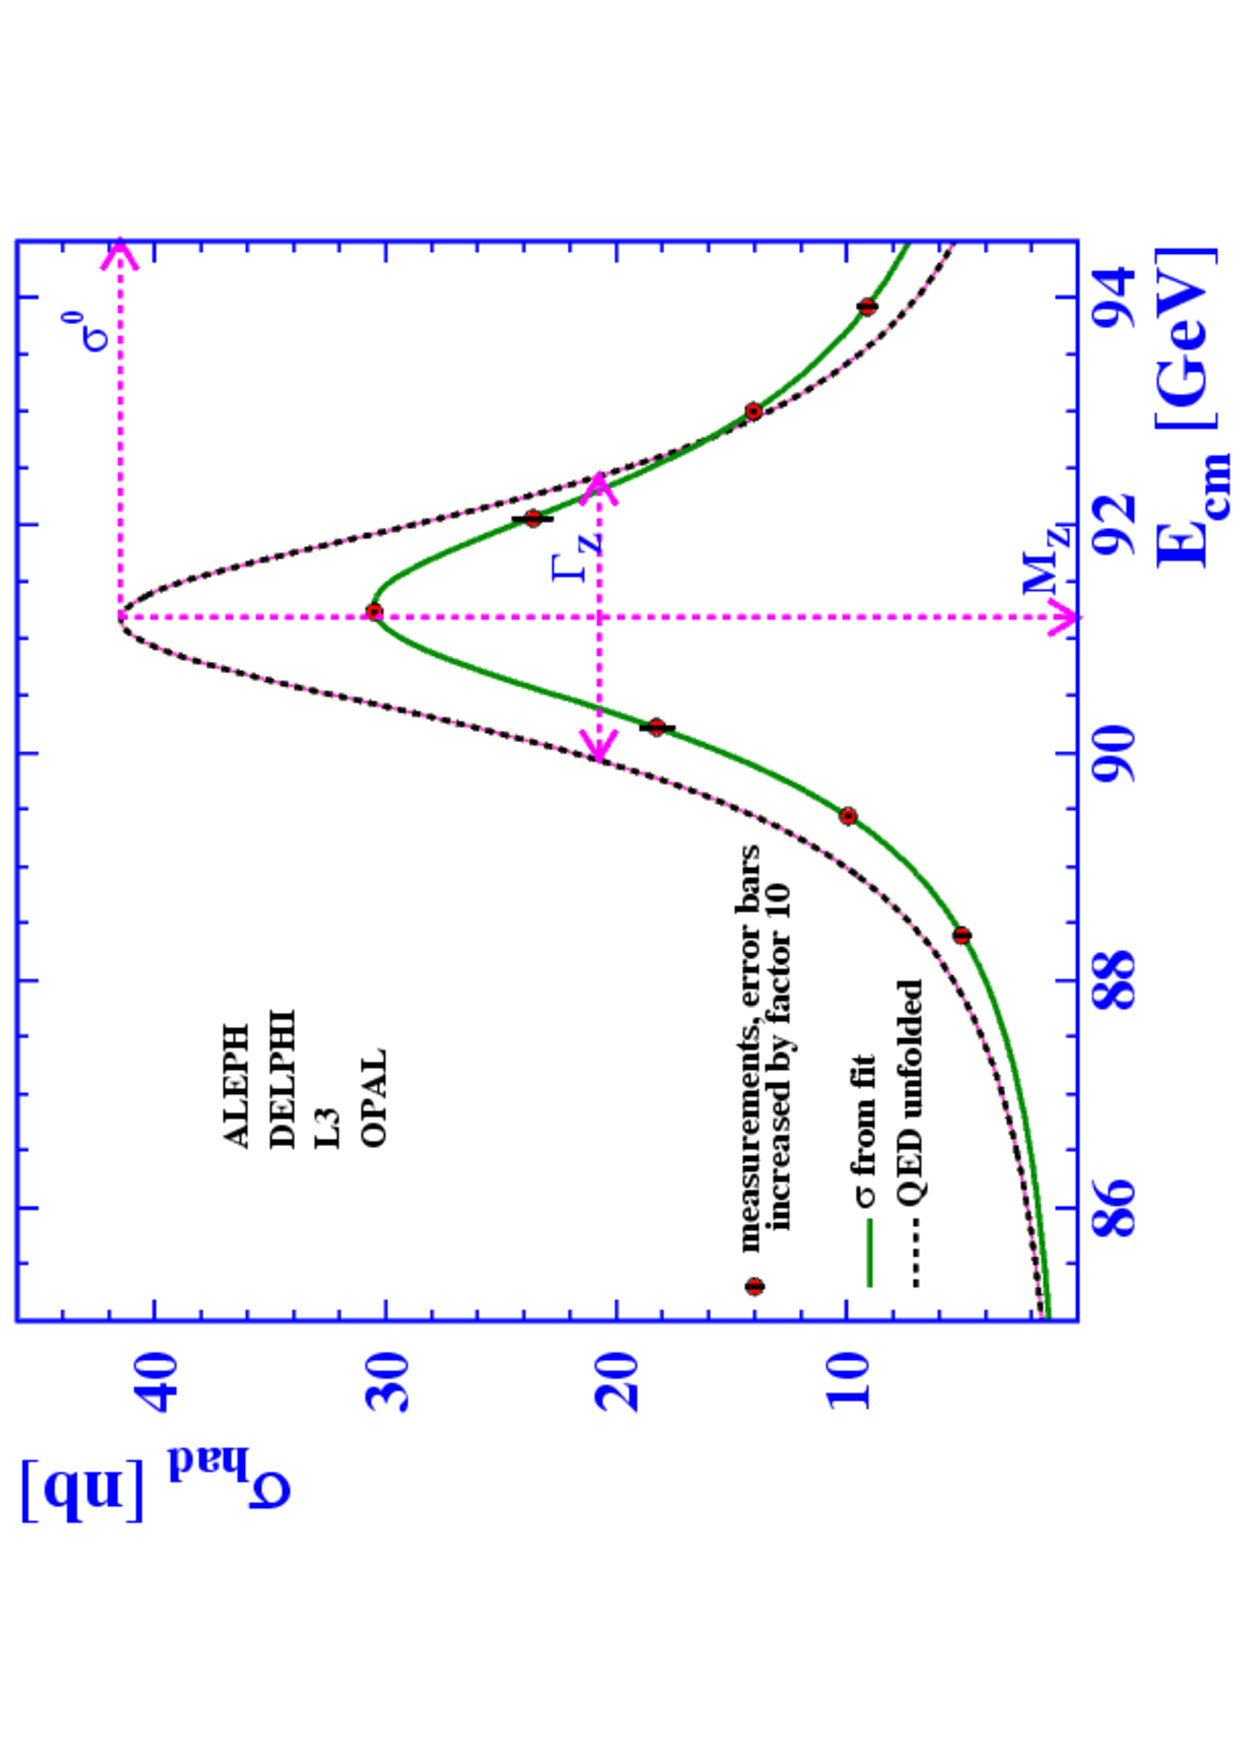
\includegraphics[width=0.6\textwidth]{fig/z_lineshape}}
\caption{The y-axis gives the cross section (proportional to probability) to produce a $Z$ particle at LEP at a given mass. To first order: ignore the green solid line, only look at the red/black broken line. (The solid green line is the uncorrected measurement of $Z$ production versus centre of mass energy of the $e^+ e^-$ beam, the red-black dotted line is $Z$ production as a function of true energy used to make the $Z$, which is subtly different because sometimes electrons and positrons radiate off photons before they collide, so that the energy available to make a $Z$ is a bit less than the beam energy.) The crucial point is that for unstable particles, we need to know both, the mean mass and the width.\label{fig:z_lineshape}}
\end{figure}
\begin{figure}
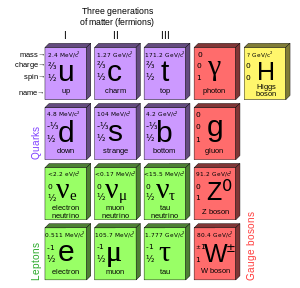
\includegraphics[width=0.6\textwidth]{fig/TheSM}
\caption{The particles of the Standard Model, and some of their basic properties, such as mass and electric charge. All electrically charged particles couple to the photon and thus interact electromagnetically. While the electric charge is given, the colour charge and weak charge are omitted in this figure. All quarks and gluons carry colour charge and thus couple to gluons (that's right, the gluons couple also to themselves), and thus interact strongly. The other particles do not. All fermions, as well as Z and W carry a weak charge, which means they couple to W and Z and can interact weakly.\label{fig:SM}}
\end{figure}


What are particles? And in particular, what are fundamental particles? We view fundamental particles a point-like objects without any internal structure. Surely, such simple objects cannot have many properties. And indeed, they are characterised fully by just a few parameters. Let us first look the 'intrinsic' properties, that are the same in any reference frame. A key property of a particle is its mass. However, for unstable particles, we need to be a bit careful, as, due to Heisenberg's uncertainty principle $\Delta E\Delta t \ge \half \hbar$, their mass (energy) is not fixed if $\Delta t \neq \infty$. The consequence of this is illustrated in Fig~\ref{fig:z_lineshape}, showing how $Z$ bosons are produced with different masses. The probability that a $Z$ will have a certain mass is described by a lineshape with two parameters: The mean mass $M$, and the width, $\Gamma$. $\Gamma$ is related to the mean lifetime of the particle, $\tau$, by 
\begin{equation}
    \tau = \frac{\hbar}{\Gamma}.
\end{equation}

Another important property of a particle is its spin. Particles with half-integer spin quantum number ($\frac{1}{2}, \frac{3}{2}, \ldots$)  are fermions, those with full-integer spin quantum number (0, 1, 2...) are bosons, which fundamentally changes their properties. Also, the spins of a particle and its decay products affect the angular distribution of the particle's decay products. 

There are further quantum numbers which can only have discrete values.They are all related to symmetries, such has how the particle behaves under parity (effectively mirror reflection), or what their wavefunction does when we swap particles with antiparticles.  We will discuss these later. Finally, the interactions of a particle with other particles are determined by its charges under the strong, the weak and the electromagnetic interaction.

And then there properties that depend on the reference frame and describe the motion of a particle. They are its four momentum (actually, if we know the mass, the 3-momentum is enough, but as mentioned above, for unstable particles the mass can vary case-by-case), and the projection of the spin onto some axis. In particle physics, we  take the projection of the spin onto the the axis defined by the particle's momentum. This quantity (multiplied by two) is called helicity. The (fairly deep) reason for this choice over the more familiar projection onto the $z$ axis will be discussed in the context of the Dirac equation.

%%Composite particles have additional properties, such as size, shape, etc. In some cases, composite particles can look like fundamental particles. This is the case when the energies involved in the interaction are such that the associated wavelengths are much larger than the size of the composite particle. This is why in atomic physics (energies of a few 10s of $eV$, the nucleus looks like a point particle to a good approximation. In nuclear physics (energies of $MeV$), nuclei are complex objects, but protons and neutrons are usually treated as structureless particles. And at the LHC (energies of several $TeV$), the proton looks like a highly complicated object formed of gluons and quarks.

Figure \ref{fig:SM} lists the fundamental particles we know about, with some of their properties. From these particle properties, we can calculate how the particles interact with each other. The tool we use for this are Feynman diagrams.

\subsection{Feynman diagrams and Feynman rules}

Feynman diagrams are a graphical representation of what is in fact a series expansion (like a Taylor expansion) of the full theory. The number of vertices in the diagram represents the order of the term in that expansion that the Feynman diagram represents. Most of the time we'll only deal with the lowest order term.

Each Feynman diagram has an exact mathematical value, which corresponds to a quantum mechanical transition amplitude, which is in general a complex number. If several Feynman diagrams contribute to the same process, their complex values need to be added up to get the full amplitude $\mathcal{M}_{fi} = A_1 + A_2 + \ldots$. A transition rate proportional to the magnitude of this number, squared:
\begin{equation}
    R \propto \left| \mathcal{M}_{fi} \right|^2
\end{equation}
The $\mathcal{M}_{fi}$ stands here for "matrix element", which is the total complex amplitude for a transition from one initial state $i$ to a final state $f$.

Evaluating Feynman diagrams can be quite a messy operation. We will here adopt the following PGA (pretty good approximation): \textbf{we will estimate Feynman diagrams \emph{ignoring spin}.} This simplifies things immensely (no gamma matrices). Our results will be good approximations as long as spin does not matter. We won't be very good at getting angular distributions right with this, but for total rates we will get good estimates in most cases. There is one significant exception in the weak interaction (helicity suppression), but we will deal with that separately. Several things will even be exactly right, such as the weak-interaction phases introduced in the context of charge-symmetry violation (see later).

\subsection{Drawing and Evaluating Feynman Diagrams}

\paragraph{Time runs from left to right in the sense that:}
\begin{itemize}
\item LHS of the diagram is the initial state
\item RHS of the diagram is the final state
\item Middle of the diagram is how it happened
\end{itemize}

\paragraph{Anti-particle arrows should point in negative time direction} for example for the $e^+e^-\to \mu^+\mu^-$ process we have
\begin{center}
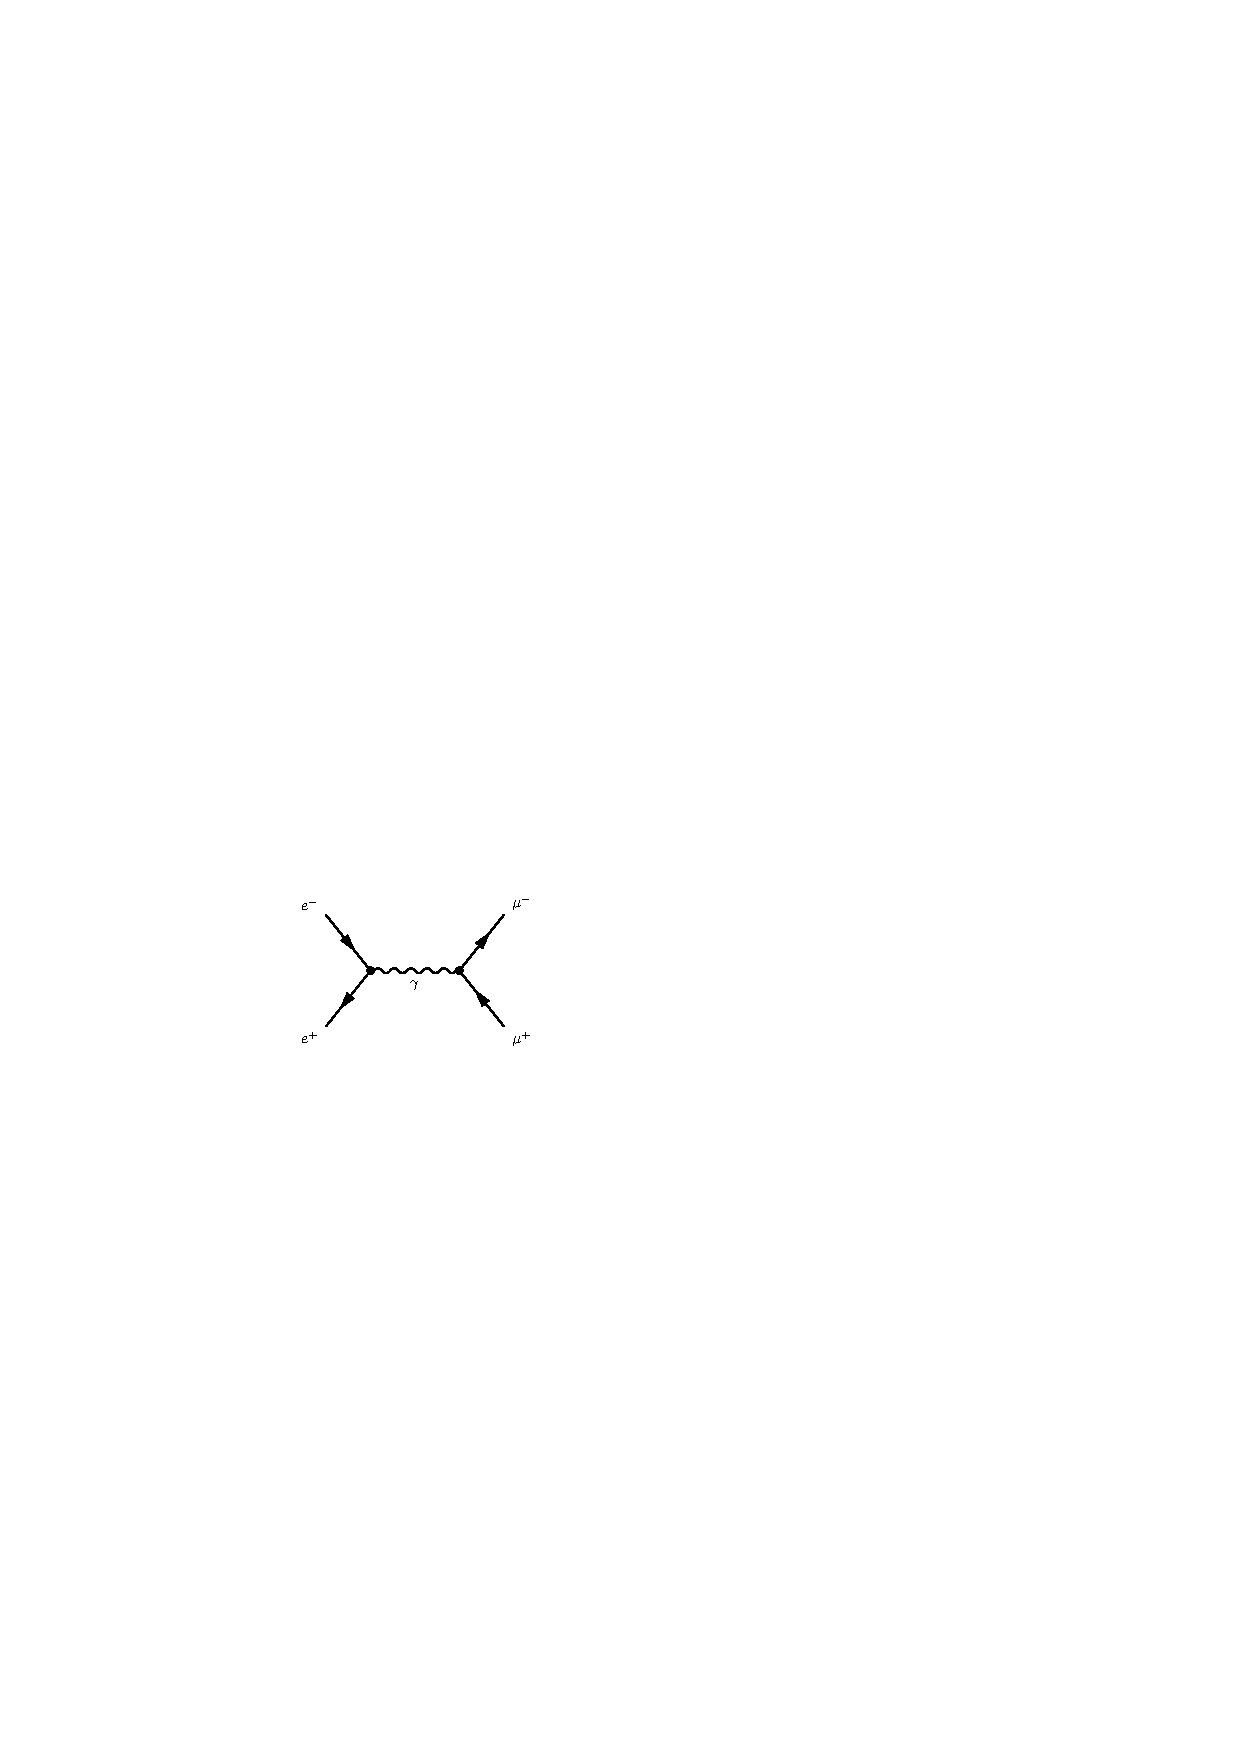
\includegraphics[width=0.5\textwidth]{fig/forcerange/eetomm.pdf}
\end{center}

\paragraph{At each vertex, 4-momenta are conserved}

\paragraph{Each vertex contributes a coupling strength factor $g$ which is proportional to the charge of the particle in question.}
In EM interactions $g$ is simply the electric charge; for an electron it's $e=\sqrt{4\pi\alpha_{EM}}$, for an upquark it's $e= - \frac{2}{3}\sqrt{4\pi\alpha_{EM}}$, for a down quark it's $e= + \frac{1}{3}\sqrt{4\pi\alpha_{EM}}$. Here $\alpha_{EM}$ is the fine structure constant $\alpha_{\rm EM}=\frac{1}{137}$. So for the example above, the process occurs at a rate proportional to $\alpha_{\rm EM}^2$.

\paragraph{Each intermediate particle (connecting 2 vertices) contributes a factor $\frac{1}{q^2 - m^2}$} where $q$ is the particle's four-momentum. The intermediate particles is virtual, and usually $E^2 \neq p^2+m^{2}$. The intermediate particle is said to be ``off-shell''. 

Below a graphical summary of our simplified (no spin) Feynman rules for QED:\\
\begin{tabular}{cc}
\textbf{Vertices} & \textbf{propagators} \\
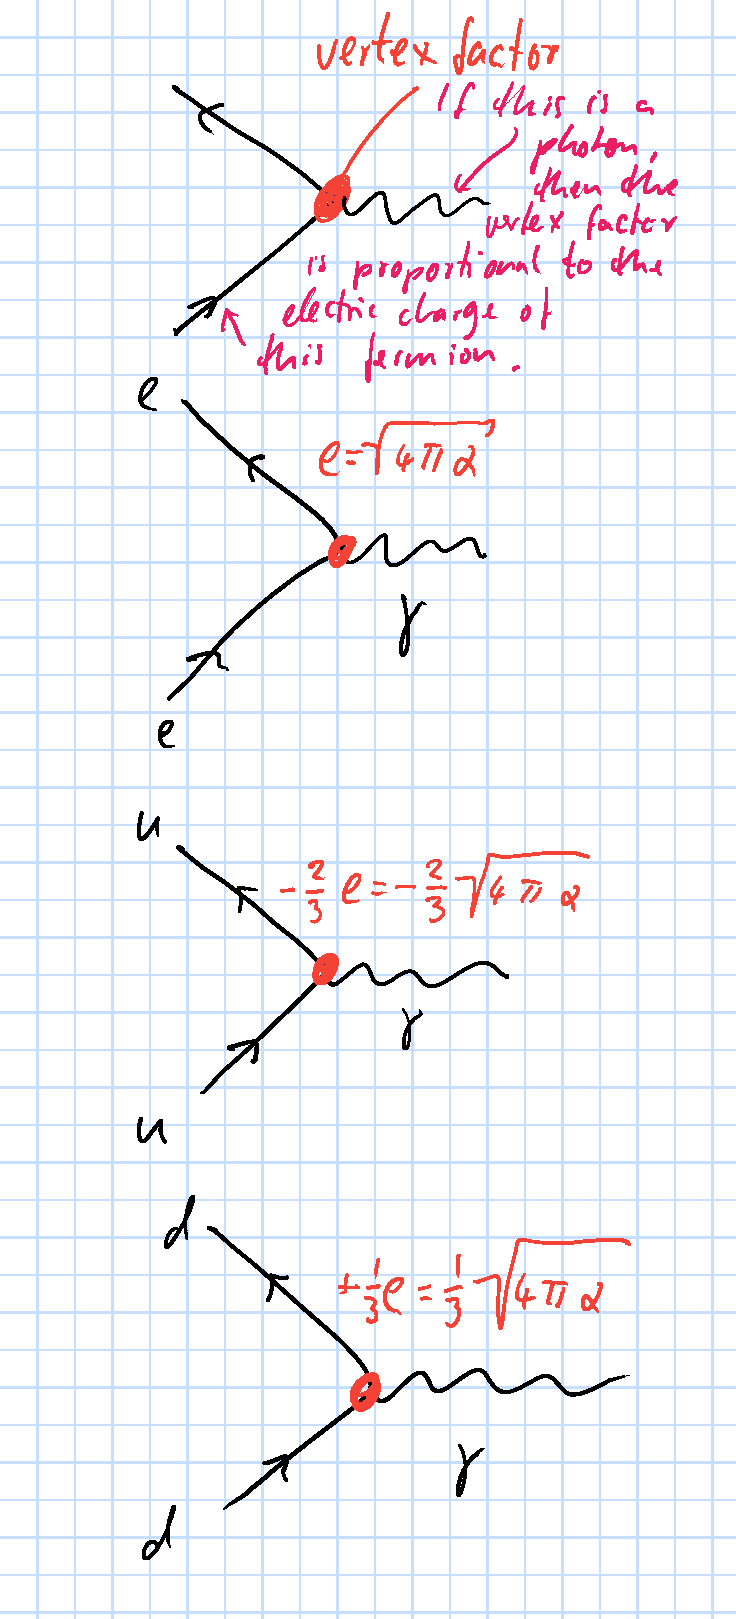
\includegraphics[width=0.4\textwidth]{fig/VertexFactorsQED}
&
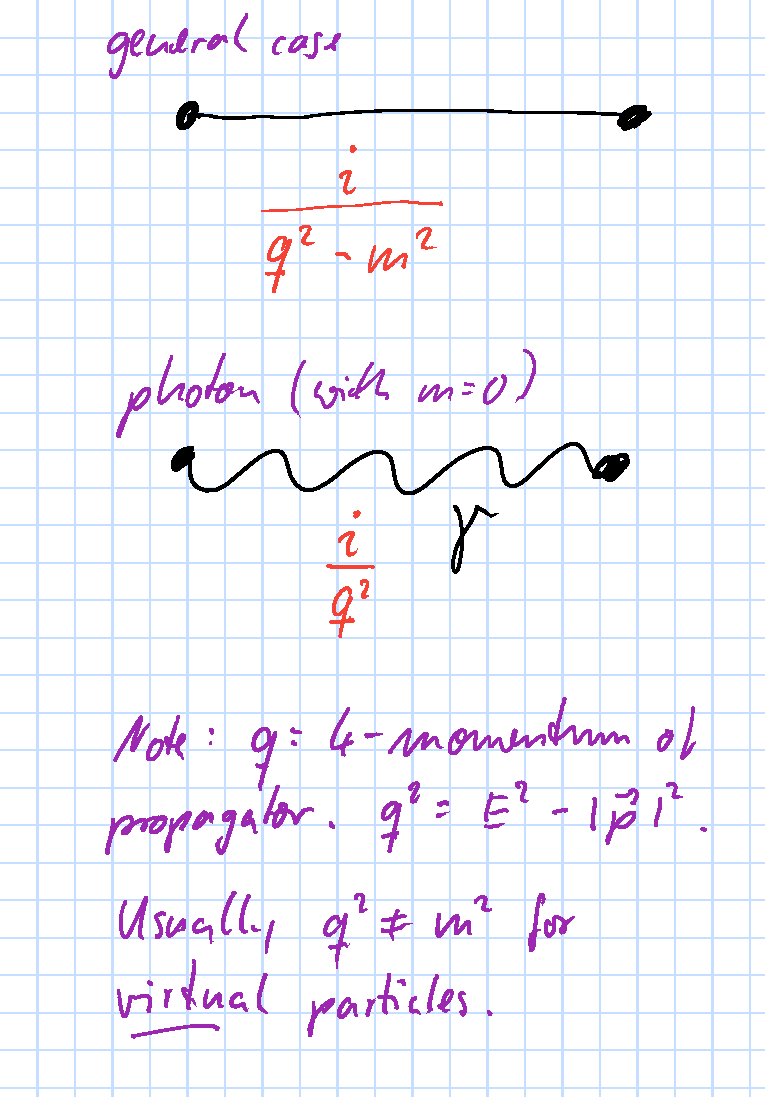
\includegraphics[width=0.58\textwidth]{fig/FeynmanPropagators}
\end{tabular}
Note that time goes from left to right and we represent antiparticles as particles going backwards in time. So an $e^-$ ($u$) is an electron (up quark) going from left two right, while an $e^+$ ($\overline{u}$) is an electron (up quark) going from right to left. You \emph{can} add labels like $\overline{u}$ next to lines going from right to left to emphasise it's an anti-particle, but you do not need to (and I usually won't), the direction of the arrow makes it all clear.

These can be stuck together to form all sorts of processes, for example $e^+ e^- \to u \overline{u}$ scattering:
\\
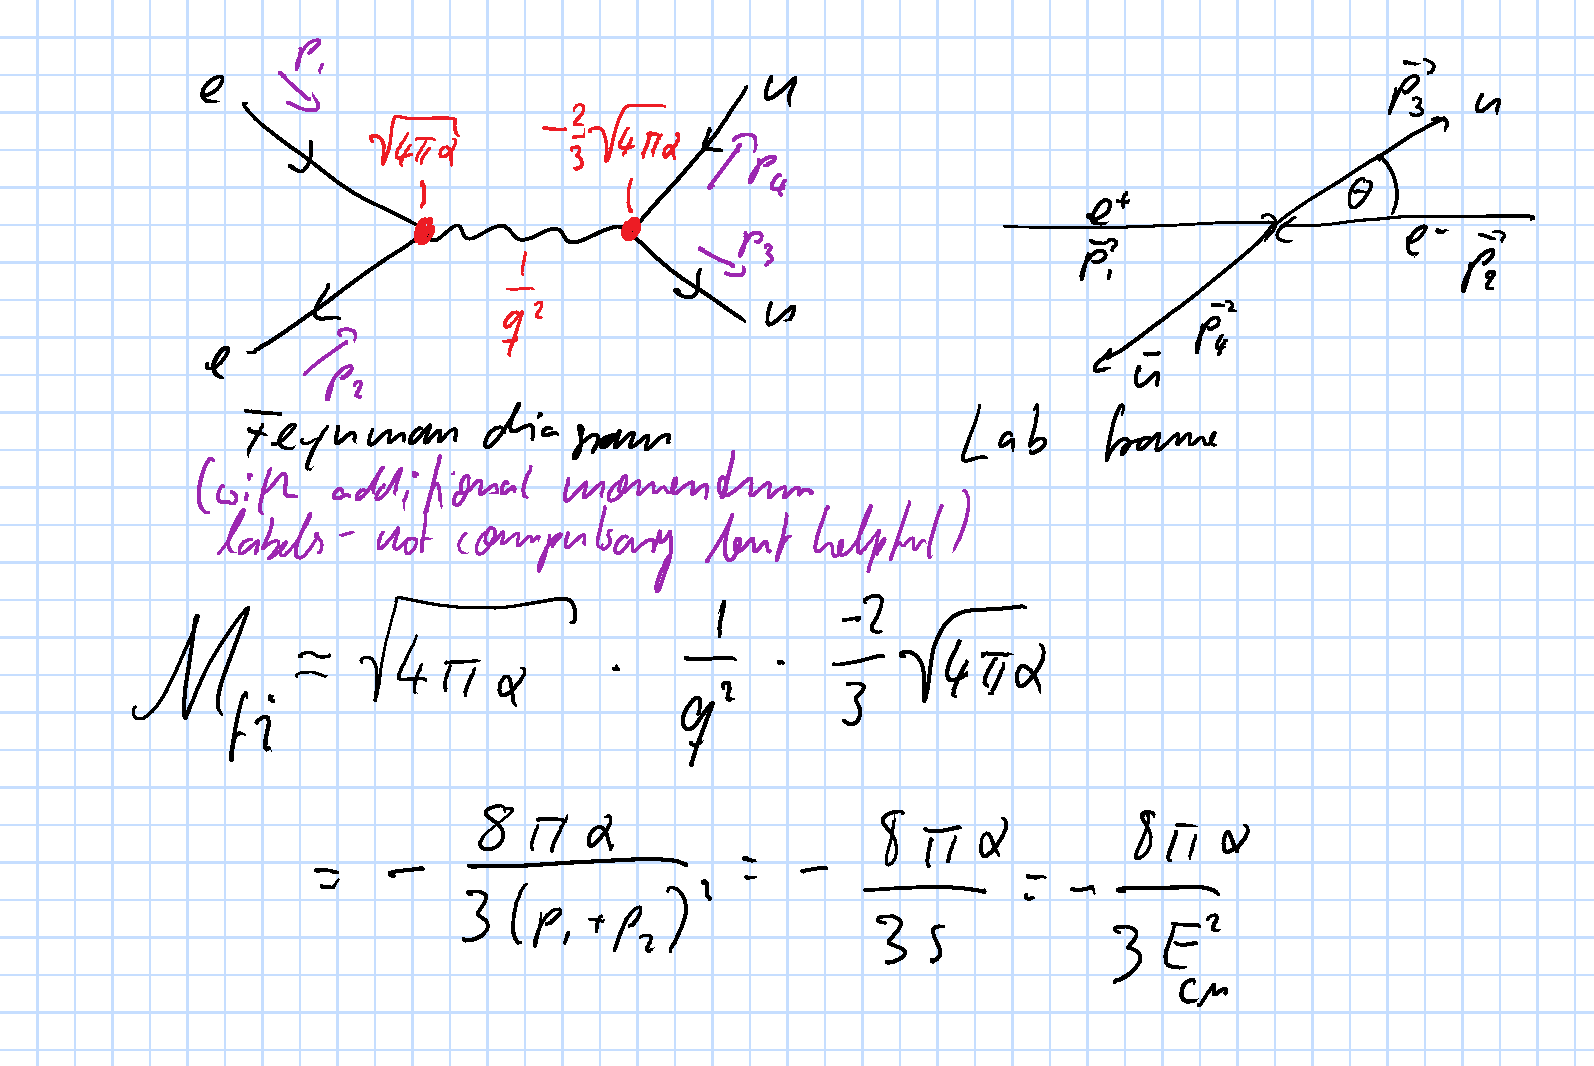
\includegraphics[width=0.9\textwidth]{fig/ExampleQED_1}

\exercise{
Draw and evaluate the Feynman diagrams in terms of the cm energy $E_{cm}=\sqrt{s}$ for these processes:
\begin{enumerate}
\item $e^+ e^- \to \mu^+ \mu^-$
\item $e^- \mu- \to e^- \mu^-$
\end{enumerate}
\inlineAnswer{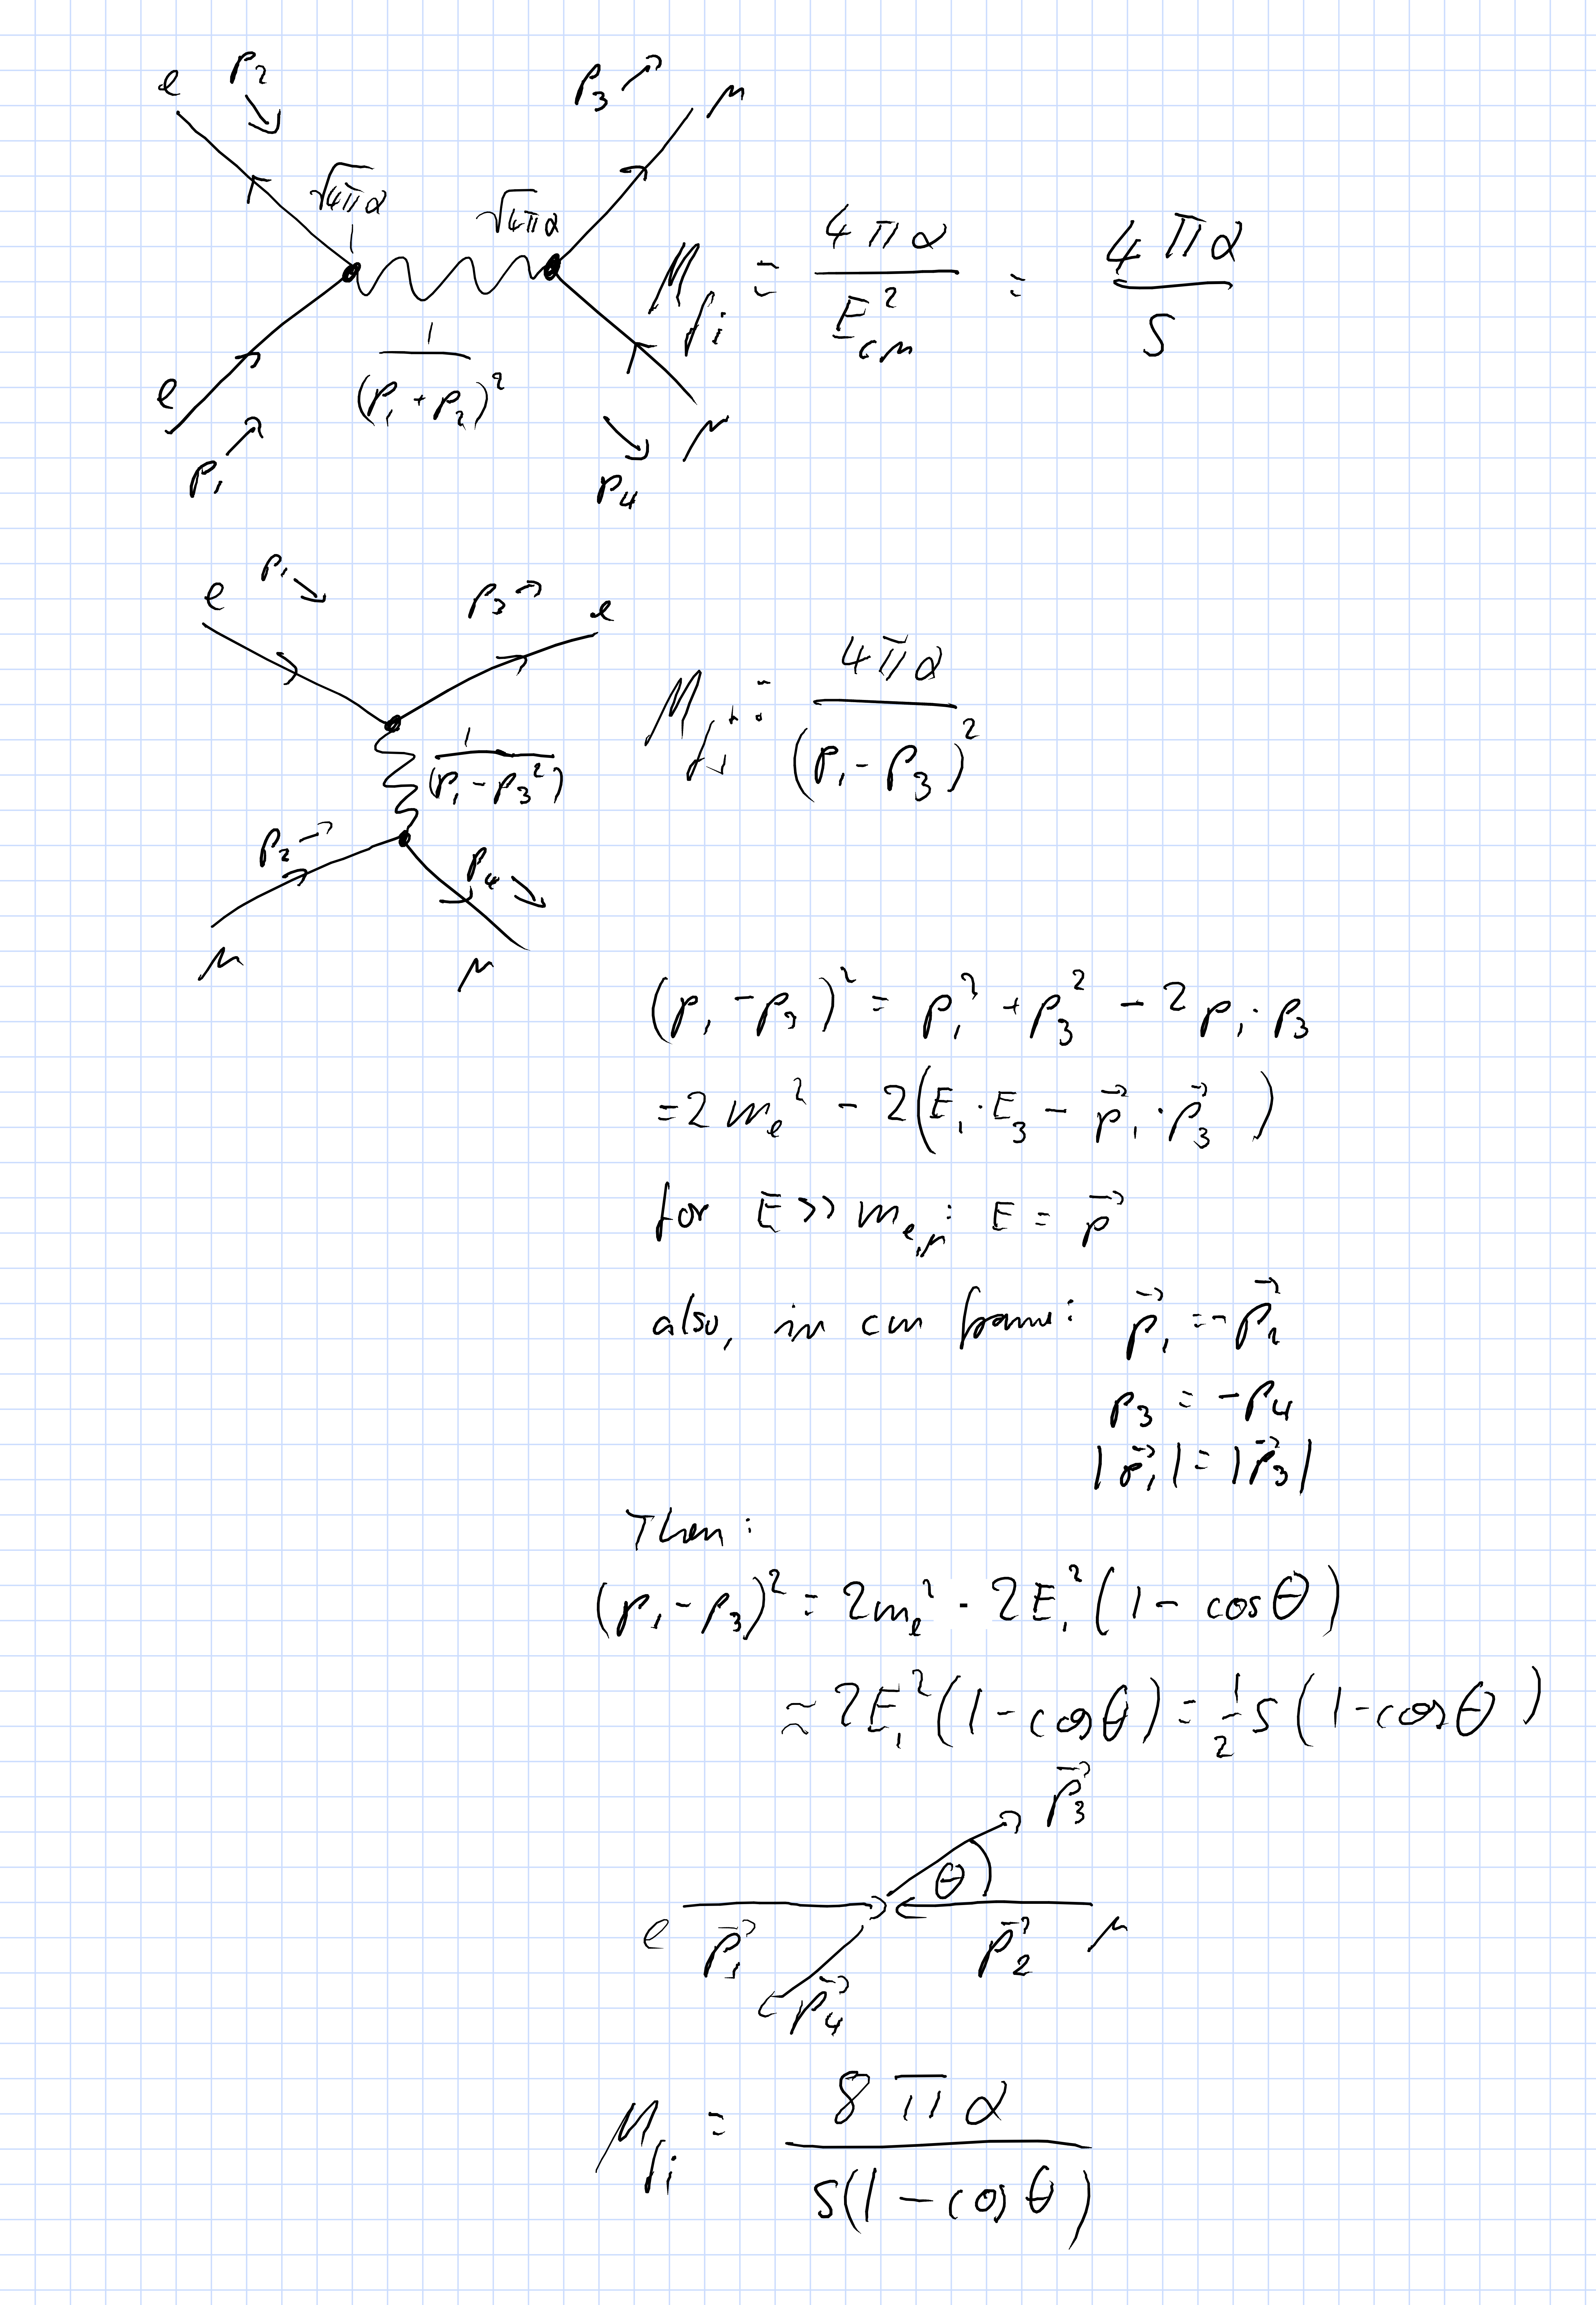
\includegraphics[width=0.8\textwidth]{fig/FeynmanFirstRevisionExercises.png}}
}

A nice introduction to drawing Feynman diagrams (and other topics in particle physics) can be found here: \href{http://www.quantumdiaries.org/2010/02/14/lets-draw-feynman-diagams}{http://www.quantumdiaries.org/2010/02/14/lets-draw-feynman-diagams}.

% \include{Scattering theory}
\section{Overview of Lorentz transformations and 4-vectors}
\label{sec:ltqs}
\subsection{Notation}
\[ x = (x^0, x^1, x^2, x^3) = (ct, x, y, z)\]
%  while $\vec{x}$ represents the space components only:
\[
\vec{x} = (x^1, x^2, x^3) = (x, y, z)
\]
Note that the symbol $x$ can refer to the four vector $x=(ct, x, y, z)$, as well as the first spatial component $x=x^1$. This has to be deduced from the context.
\subsection{Lorentz transformations}
Lorentz transformations transform between two frames that have a constants velocity relative to each other. They includes rotations, shifts and boosts.
The transformation for a boost in $x$ direction (with $\beta = v/c, \gamma = \frac{1}{\sqrt{1-\beta^2}}$) is given by:
\begin{equation}
\vIV{ct^{\prime}}{x^{\prime}}{y^{\prime}}{z^{\prime}}= 
      \left( \begin{array}{cccc} \gamma       & -\beta\gamma &  0  & 0  \\ 
                                 -\beta\gamma &  \gamma      &  0  & 0  \\
                                        0     &    0         &  1  & 0  \\
                                        0     &    0         &  0  & 1
             \end{array} \right)\vIV{ct}{x}{y}{z} 
\end{equation}
and in the y-direction
\begin{equation}
\vIV{ct^{\prime}}{x^{\prime}}{y^{\prime}}{z^{\prime}}= 
      \left( \begin{array}{cccc} \gamma       &   0 & -\beta\gamma &  0  \\ 
                                     0        &   1 &   0 & 0  \\
                                 -\beta\gamma &   0 & \gamma     & 0  \\
                                        0     &    0         &  0  & 1

             \end{array} \right)\vIV{ct}{x}{y}{z} 
\end{equation}
and in the z-direction
\begin{equation}
\vIV{ct^{\prime}}{x^{\prime}}{y^{\prime}}{z^{\prime}}= 
      \left( \begin{array}{cccc} \gamma       &   0 & 0 & -\beta\gamma  \\ 
                                     0        &   1 & 0 & 0  \\
                                     0        &   0 & 1 & 0  \\
                                 -\beta\gamma &   0 & 0  & \gamma
             \end{array} \right)\vIV{ct}{x}{y}{z} 
\end{equation}
Note that rotations are also a kind of Lorentz transformation, but one that only affects the space component. Below a rotation about the $z$ axis:
\begin{equation}
\vIV{ct^{\prime}}{x^{\prime}}{y^{\prime}}{z^{\prime}}= 
      \left( \begin{array}{cccc}      1     &  0 &  0  & 0  \\ 
                                0     &  \cos\theta  &  \sin\theta  & 0  \\
                                0     &  -\sin\theta & \cos\theta  & 0  \\
                                0     &    0         &  0  & 1
             \end{array} \right)\vIV{ct}{x}{y}{z} 
\end{equation}
A general Lorentz transformation is a combination of rotations, boosts, and co-ordinate shifts as in $x' = x + \delta x$.

\subsection{Four Vectors}
Four-vectors are defined as objects that transform under Lorentz transformations like  $(c\mathit{\Delta t}, \mathit{\Delta x}, \mathit{\Delta y}, \mathit{\Delta z})$, i.e. differences in $ct, x, y, z$. The most important four-vectors are:
\begin{align}
  \Delta x &= \vIV{c\Delta t}{\Delta x}{\Delta y}{\Delta z}
& dx &= \vIV{c\,dt}{dx}{dy}{dz}
& p &= \vIV{E}{cp_x}{cp_y}{cp_z}
& \partial &= \vIV{\partdbyd{}{(ct)}}{-\partdbyd{}{x}}{-\partdbyd{}{y}}{-\partdbyd{}{z}}
\end{align}
If we consider only rotations and boosts ("proper" Lorentz transformations), and not shifts (like $x' = x + \delta x$), then (ct, x, y, z) also transforms like a 4-vector.

The above leads to the following important relationships:
\begin{align}
\label{eq:EandP_fromBetaGammaM}
E &= \gamma m c^2 & \left|\vec{p}\right| = \beta \gamma m c
\end{align}
where $\beta$ is the speed of the particle, and $\gamma = 1/\sqrt{1-\beta^2}$
Note: In these notes, $m$ always refers to the rest mass of a particle, in some books called $m_0$. We do not use the concept of a speed-dependent mass $m_{\mathrm{some\;other\;books}}=\gamma m$, instead we write out the $\gamma$ factor explicitly as in $E=\gamma mc^2$.
\\\exercise{
Derive equation~\ref{eq:EandP_fromBetaGammaM} from $E=mc^2$ for a particle at rest.
\vspace{1ex}\\
\rotatebox{180}{\parbox{0.9\textwidth}{Answer: Without loss of generality we can pick a coordinate system where $\vec{p} = (p_x, 0, 0)$, and the particle moves with speed $v_x$. Boosting from the system where the particle is at rest to our system corresponds to a boost of $-\beta_x = -v_x/c$ (note the $-$ sign). Then
\begin{equation*}
      \left( \begin{array}{cccc} \gamma       &  \beta_x\gamma &  0  & 0  \\ 
                                 \beta_x\gamma &  \gamma      &  0  & 0  \\
                                        0     &    0         &  1  & 0  \\
                                        0     &    0         &  0  & 1
             \end{array} \right)\vIV{mc^2}{0}{0}{0} 
= \vIV{\gamma mc^2}{\beta_x\gamma mc^2}{0}{0} 
\end{equation*}
So $E = \gamma mc^2$ and $|\vec{p}| = p_x = \beta_x\gamma mc^2 / c = \beta_x\gamma mc $.}}
}
\\\exercise{What's the speed of a particle with energy $E=\un{1}{GeV}$ and momentum $\vec{p} = (0, 0, \un{0.9}{GeV}/c)$?
\rotatebox{180}{Answer: $v = 0.9c$}
}
\subsection{Invariants and dot products}
Dot products between four vectors are defined like this
\begin{equation}
A \cdot B = A^0 B^0 - \vec{A} \cdot \vec{B}
\end{equation}
are Lorentz invariant, i.e. they are the same in any coordinate system. This also works for $A \cdot A$, giving for each four vector $A$ one invariant $A^2$.
Especially important is
\begin{equation}
s = p^2 = p \cdot p = E^2 - c^2 \vec{p}^2
\end{equation}
In the centre of mass frame, $\vec{p}=\vec{0}$, so we see that $\sqrt{s}=E_{cm}$, is the centre-of-mass energy. For an individual particle with momentum $p$, $p^2=(mc^2)^2$ where $m$ is the particle's mass. This is important enough to write down again:
\begin{align}
(mc^2)^2 &= E^2 - (pc)^2 &\mathrm{or}\; E^2 &= (mc^2)^2 + (pc)^2
\end{align}

\exercise{\\
    Go over this interesting computation at your own time:\\
    Consider a particle moving a differential line element $d\vec{x}$ in time $dt$. The differential four interval
    \begin{equation}
      ds^2 \equiv dx\cdot dx = c^2dt^2 - \left|d\vec{x}\right|^2 = c^2dt^2 \left(1-\beta^2\right)
    \end{equation}
    is also an important invariant. (Beware of the potentially confusing re-use of the variable $s$ in this context.) In the rest frame of the particle, $d\vec{x}=0$, and we identify $ds$ with the differential of the proper time
    \begin{equation}
      d\tau = dt \sqrt{1-\beta^2} = \frac{dt}{\gamma_u};
      \label{eq:proptime}
    \end{equation}
    $\tau$ is the proper time of the particle, which is the same as the time of the particle at rest. Time intervals observed from a moving co-ordinate system are stretched by a factor of $\gamma$ relative to the time in the restframe - the famous time dilation.
}
\\\exercise{
\begin{enumerate}
\item A particle  has energy $E=\un{1.118}{GeV}$ and momentum $\vec{p}=(0, 0, \un{1}{GeV/c})$. What is its mass?
\item The same particle is observed in reference frame $S'$ with momentum $\vec{p}'=(\un{0.5}{GeV/c}, \un{0.5}{GeV/c}, 0)$. What is its energy, now?
\item In frame $S'$, the particle exists for $\un{1}{fs}$ before it decays. How long did it exist in its own restframe? (Hint: use $E=\gamma m c^2$.)
\end{enumerate}
\rotatebox{180}{Answers: $m=\un{0.5}{GeV/c^2}$, $E'=\un{0.866}{GeV}$, $t_{\mathrm{rest}} = \un{0.577}{fs}$}
}

\section{Particle kinematics}
In Sec.~\ref{sec:ltqs} we discussed 4-momentum and how
it transform under a Lorentz-boost. One important point
is that energy and momentum conservation still applies. These
conservation rules are different to frame invariance, and rather
refer to conservation in time ie
\[
E_{\rm TOTAL}=E_{1}+E_{2}+...+E_{n}
\]
and 
\[
\vec{p}_{\rm TOTAL}=\vec{p}_{1}+\vec{p}_{2}+...+\vec{p}_{n},
\]
are both conserved quantities at any point in space and time.
However:
\[
m_{\rm TOTAL}=m_{1}+m_{2}+...+m_{n},
\]
is NOT conserved, but IS invariant under Lorentz transformations.

\noindent Let us consider a couple of applications of energy-momentum conservation
in particle collisions. In particle physics,
\noindent 
\[
m^{2}=p_{\rm TOTAL}\cdot p_{\rm TOTAL}=E^{2}_{\rm TOTAL}-\vec{p}^{2}_{\rm TOTAL},
\]

is used to quantify the energy involved in a collision. As $m^{2}$ is a Lorentz invariant quantity, 
it is equivalent to the total energy squared in a frame where $\vec{p}^{2}_{\rm TOTAL}=0$ 
i.e the Centre of Mass (CoM) frame. Therefore we can define $s\equiv m^2$ and  thus $\sqrt{s}$ is the CoM energy.

\paragraph{Example 1: ``Fixed target'' collision}
\begin{center}
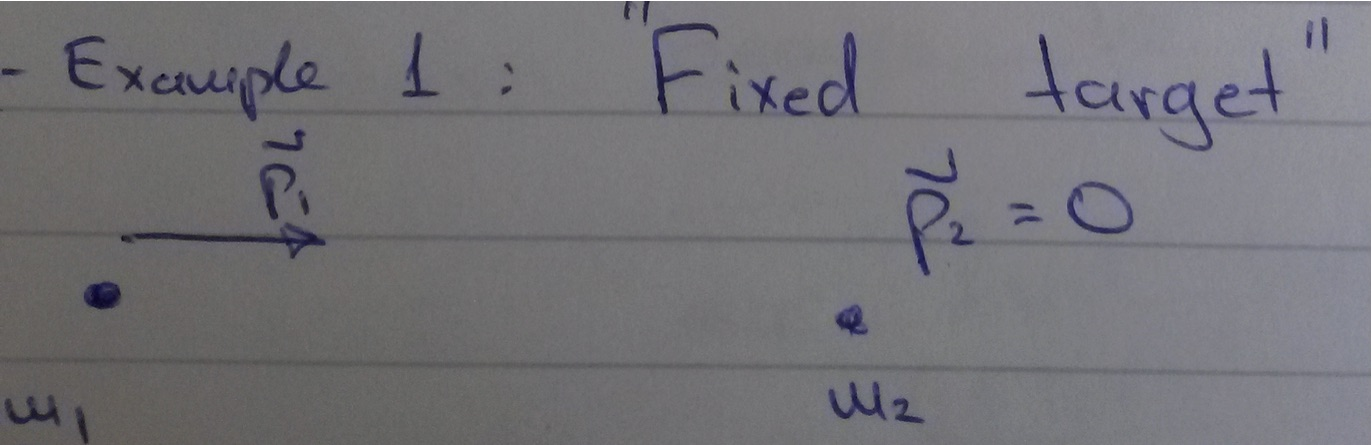
\includegraphics[width=0.5\textwidth]{fig/collisions/collisions_example1.jpg}
\end{center}

In this example
\[
s=(E_{1}+E_{2})^{2}-(\vec{p_1})^2.
\]
since $\vec{p_2}=\vec{0}$. Remembering 
that $|p_1|^2=E_{1}^{2}-m_{1}^{2}$ (using natural units) and rearranging, we get
\[
E_{1}=\frac{s-m_{1}^{2}-m_{2}^{2}}{2m_{2}}.
\]
\noindent Therefore in a fixed target collision, in order to achieve a CoM 
energy $\sqrt{s}$, one needs a beam of energy as given above.  If we make the assumption that the required $s$ is much larger than $m_{1}^2$ and $m_{2}^{2}$, then the expression for the beam energy of a fixed target collider reduces to\footnote{Particle beams
consist of electrons or protons or pions or kaons. All these particles have masses $<1$~GeV.
The mass of the target does not refer to the macroscopic mass of the whole target block, but rather to the microscopic mass of nucleus with which the proton interacts. For all practical purposes the mass of the target can be considered as the atomic mass of the nucleus. Depending on the target, the mass can vary between $\sim 1$~GeV for a hydrogen target to $\mathcal{O}(10)$~GeV for a beryllium target or $\mathcal{O}(100)$~GeV for a molybdenum target.}:
\begin{equation}
\label{eq:e_fixed_target}
E_{1}\sim \frac{s}{2m_{2}}.
\end{equation}

\paragraph{Example 2: ``Particle collider''}
\begin{center}
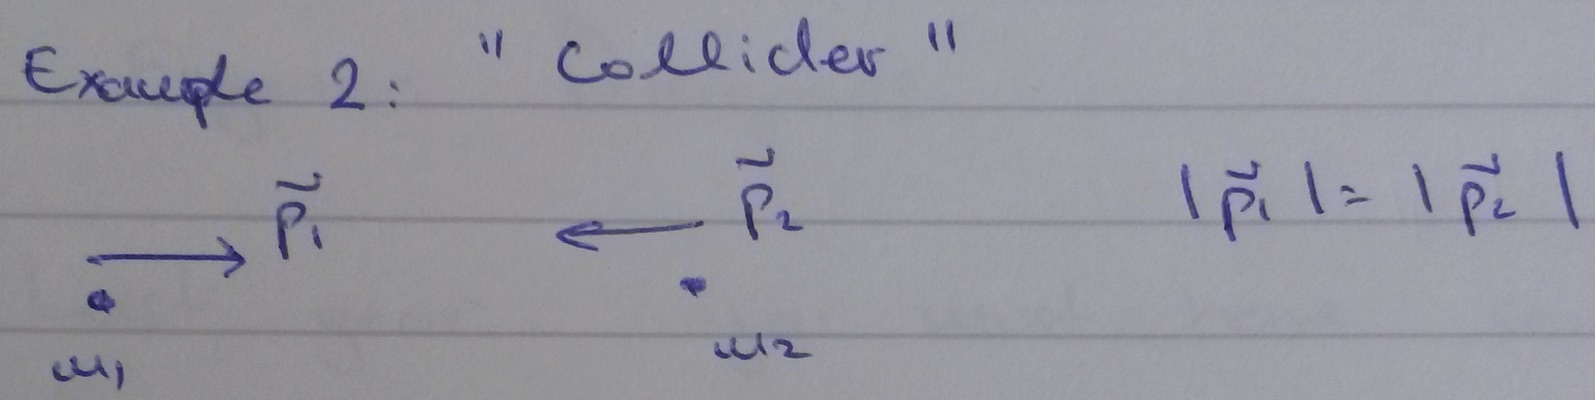
\includegraphics[width=0.5\textwidth]{fig/collisions/collisions_example2.jpg}
\end{center}
Consider two colliding beams with $\vec{p_1}=-\vec{p_2}$.
In this case:
\[
s=(E_{1}+E_{2})^{2}.
\]
Using  $|p_1|^2=|p_2|^2$ we have:
\[
E_{1}^{2}-E_{2}^{2}=m_{1}^{2}-m_{2}^{2}
\]
Therefore we can replace $E_2$ in favour of $E_1$ and get:
\[
E_1=\frac{s+m_{1}^{2}-m_{2}^{2}}{2\sqrt{s}}
\]
Under the assumption that $s \gg m_{1}^2,m_{2}^2$, we can write:
\begin{equation}
\label{eq:e_collider}
E_{1}\sim \frac{\sqrt{s}}{2}.
\end{equation}

Consider now that we want to build an accelarator which produces collisions
at $\sqrt{s}=13$000~GeV (13~TeV), very much like the Large Hadron Collider running
currently at CERN. Given Eq.~\ref{eq:e_collider}, one would require a beam energy of 6.5~TeV per beam. 

If however we were to use a ``fixed-target'' type facility, then using Eq.~\ref{eq:e_fixed_target}, where we consider a hydrogen target in which case $m_{2}\sim 1$~GeV, the required beam energy would be $E_{1}=\frac{13000^2}{2\times1}\sim84.5$~PeV!!

These two examples illustrate why if one is after high energies, it is much more efficient to accelerate and collide two beams rather than whack a single beam onto a target. If however one is interested in a large number of collisions (high intensity rather than high energy) then the most efficient way is a ``fixed target'' configuration.

\exercise{
When the Large Hadron Collider started colliding beams at $\sqrt{s}=13$~TeV, some members of the press claimed that: ``The Large Hadron Collider produces the highest energy collisions in our solar system ''. 

Cosmic rays are high energy charged particles originating outside our solar system. They have been observed to have energies up to $10^{20}$~eV. By considering the collision of the most energetic cosmic ray with stationary hydrogen gas in the universe decide whether the statement was correct.
\rotatebox{180}{Answer: Cosmic ray on Hydrogen $\sqrt{s}\sim450$~TeV.
%Hydrogen gas means the target particle is\\ a proton of mass $m_p\sim 1$~GeV. So for a fixed target collision we have $\sqrt{s}\sim\sqrt{2E m_p}$ Therefore $\sqrt{s}\sim\sqrt{1\times10^{20}\times1\times10^9}\sim450~$~TeV,\newline compared to LHC's 13~TeV so the statement was incorrect.
}
}


\section{Natural units*}
\label{sec:naturalUnits}
We will usually use ``natural'' units with 
\[
c=\hbar=1.
\]
 Disclaimer: If inconsistencies are found in the notes in terms of missing/additional
 factors of $\hbar$ or $c$ please let me know. The person that spots the most errors
 will be in for a prize (nothing too special, more about the 
 feeling of satisfaction and pride...) 
 
 Amongst other things, this implies that time and length have the same
 units. From
\[
  E^2 = (cp)^2 + (mc^2)^2,
\]
 which simplifies to
\[
  E^2 = p^2 + m^2
\]
 in our system of units, we see that energy, momentum and mass
 have the same units. The relationship between wavelength and
 momentum of the photon:
\[
   p = \hbar \frac{2\pi}{\lambda}
\]
 implies that the units for momentum are inverse to those for
 distance. If we choose \units{GeV} as our energy unit, we get:
\begin{itemize}
  \item \units{GeV} as unit for mass, energy, momentum
  \item \units{GeV^{-1}} as unit for time and distance
\end{itemize}

The trick for translating from natural units, where $\hbar=c=1$, to
other systems, is to multiply any part of the expression/formula in
natural units with factors of $1$ expressed in terms of $\hbar$, $c$,
$c^2$, $\hbar c$, etc, until the expression has the correct units in
both systems. Remember that the units of $\hbar$ are [Energy]$\times$[Time] (e.g. \units{J\, s} or \units{MeV \, s} in SI units) while the units of $c$ are [Distance]/[Time]. Their product has units of [Energy]$\times$[Distance]. A relationship that is particularly useful for translating those units back to SI
 units is
\[
  \hbar c = \un{196}{MeV\,fm}.
\]
It's worth remembering this, or at least
\[
  \hbar c \approx \un{200}{MeV\,fm}.
\]

Let's for example translate the lifetime of a particle
from \units{MeV^{-1}} into seconds. The width of the \prt{\phi} particle is
$\Gamma = \un{4.458}{MeV}$, so, in our system of units, its lifetime
is $\tau = 1/\Gamma=\un{0.2243}{MeV^{-1}} =\un{0.2243}{MeV^{-1}} \hbar
= \un{0.2243}{MeV^{-1}} \hbar c/c$. The expression on the right is
exactly the same as the one on the left in our system of units, but it
also has the correct units in the SI system (time). Hence
 \begin{eqnarray*}
\tau &=&       \un{0.22}{MeV^{-1}} \hbar c/c                 \\
     &\approx& \un{0.22}{MeV^{-1}} \cdot \un{200}{MeV\,fm} /c      \\
     &\approx&       \un{44}{fm} /c                                \\
     &\approx& \un{44/3 \cdot 10^{-15}\cdot 10^{-8}}{s}  \\
     &\approx&        1.5 \cdot 10^{-22} \units{s}
\end{eqnarray*}

\exercise{
Translate the following recipe into natural units:
"Take 2 eggs, 500g of flour and a pint of milk. Mix for 10 min."
\vspace{1ex}\\
\rotatebox{180}{\parbox{0.9\textwidth}{
\begin{itemize}
\item 2 is just a number and remains invariant under the unit change.
\item 500$g$ is a mass, we want to know what that is in energy units, so we need to calculate: $mc^2 = \un{0.5}{kg}\cdot \un{9\cdot 10^{16}}{m^2/s^2} = \un{4.5\cdot 10^{16}}{J}$. Now multiply by $e/e$: $\un{4.5\cdot 10^{16}}{e J/e}$. Use $J/C = V$ and $e=\un{1.6 \cdot 10^{-19}}{C}$ to get
\un{2.8\cdot 10^{35}}{eV} of flour.
\item 1pint refers to a volume of \un{568}{cm^3}. We will measure volume in terms of $(eV)^-3$. We'll use that $\hbar c$ has units of [energy]$\times$[length]. So...
$\un{568\cdot 10^{-6}}{m^3} / (\hbar c)^3 = 
\un{5.68\cdot 10^{-4}}{m^3} / (\un{8\cdot 10^6}{MeV^3 fm^3})
=\un{0.71\cdot 10^{-4-6+45}}{MeV^{-3}} = \un{0.71\cdot 10^{35}}{MeV^{-3}}$
\item We want to multiply \un{600}{s} with factors of $\hbar$ and $c$ until we get inverse energy units. This is achieved by dividing by $\hbar$, which has units [energy]$\times$[time]. So we get $\un{600}{s} / \hbar$, which we calculate again with the $\hbar c$ trick, $\un{600}{s} /\hbar c/c = 600s /(\un{200}{MeV\,fm}) \cdot (3\cdot 10^8 m/s) = \un{9\cdot 10^{22}}{MeV^{-1}}$. 
\end{itemize}
So the solutions is:
"Take 2 eggs, a mass of \un{2.8\cdot{10^{35}}}{MeV} of flour and a volume of \un{0.71\cdot 10^{35}}{MeV^{-3}} of milk. Mix for \un{9\cdot 10^{22}}{MeV^{-1}}"
}}
}

Further discussion on natural units that goes beyond what is examinable
can be found in the Appendix.


\newpage

%% Week 3
\section{The Dirac equation and anti-particles}
Last year you saw processes of the form:
$e^+e^-\to \mu^+\mu^-$ or $e^+e^-\to q\bar{q}$ where $e^+$ is the anti-particle
of the $e^-$, $\mu^+$ the anti-particle of the $\mu^-$ and $\bar{q}$ the anti-particle of $q$. However, so far the Schr\"odinger equation says nothing about anti-particle states. 

\begin{figure}
\caption{Paul A.M.~Dirac}
\begin{tabular}{cc}
\parbox{0.32\textwidth}{
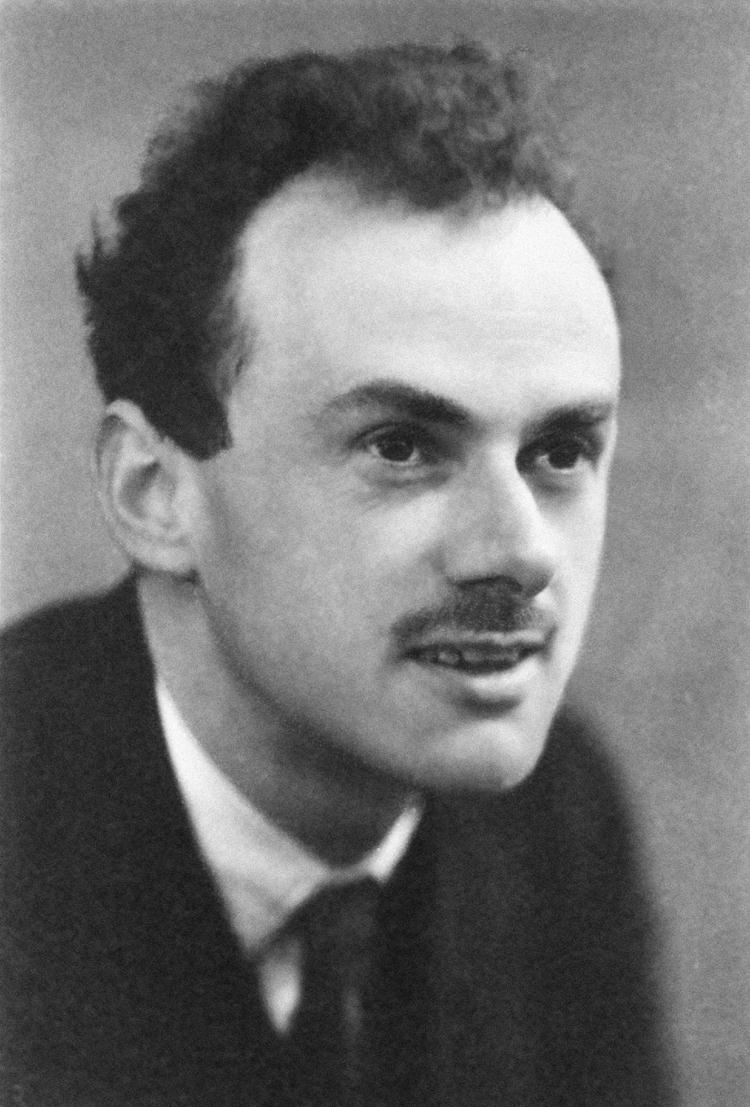
\includegraphics[width=0.3\textwidth]{fig/dirac/Dirac_4.jpg}
}&
\parbox{0.66\textwidth}{\textsf{\small
    ``Paul A.M.~Dirac studied Electrical engineering and Mathematics at the {\bf University of Bristol} before going to Cambridge for his PhD. In 1928 he developed a relativistic form of the wave equation which implied the existence of anti-matter and also provided theoretical justification for intrinsic angular momentum (spin). He was awarded the Nobel Prize in 1933 together with Schr\"odinger.'' 
}}
\end{tabular}
\\  \textsf{Source: \httplink{https://en.wikipedia.org/wiki/Paul\_Dirac}}
\end{figure}

In fact the main problem with the Schr\"odinger is that in its current form it does not account for relativistic effects. Dirac tried to address this issue in order to formulate a relativistic quantum mechanical description of the hydrogen atom.

%\paragraph{The Hydrogen atom}
%Consider the hydrogen atom whose energy levels are given by
%\[
%|E_n|=\left(\frac{e^2}{4\pi\epsilon_0}\right)^2\frac{m_{e}}{2\hbar^2}\frac{1}{n^2}.
%\]
%Equating this energy to the kinetic energy of the electron (Virial theorem) we arrive at the expression:
%\[
%v_{e}\sim \frac{e^2}{4\pi\epsilon_0\hbar}=\frac{c\alpha}{n^2},
%\]
%\noindent where $\alpha=\frac{1}{137}$ is the fine-structure constant.
%Therefore at the ground state ($n=1$), the electron speed is $\sim 1\%$ of the speed of light so relativistic effects start to have a small but measurable effect.

\subsection{Towards a relativistic form of Schr\"odinger's equation}

Schr\"odinger's equation in 3 dimensions for a free massive particle is given by:
\begin{equation}
\label{eq:schrodinger_free_massive}
-\frac{\hbar^2}{2m}\vec{\nabla}^2\psi=i\hbar\frac{\partial\psi}{\partial t}
\end{equation}
It can be shown that this equation is not Lorentz-covariant ie under a Lorentz transformation, Eq.~\ref{eq:schrodinger_free_massive} does not hold in all inertial frames. In other words, it cannot be written in terms of 4-vector or scalar quantities.

An easy way of seeing this, is that the left-hand-side of Eq.~\ref{eq:schrodinger_free_massive} has a $2^{\rm nd}$ order space derivative but the right-hand-side has a $1^{\rm st}$ order time derivative.

\paragraph{Momentum and Energy operators}
The solution to Eq.~\ref{eq:schrodinger_free_massive} can be written as
\[
\psi(\vec{x},t)\propto e^{\frac{i}{h}(\vec{p}\cdot\vec{x}-E t)}.
\]
By inserting into Eq.~\ref{eq:schrodinger_free_massive} one ends up with the relation:
\[
\frac{p^2}{2m}\psi=E\psi.
\]
By inspection therefore we can write\footnote{Note that a more formal derivation of these operators exists by considering the effect of infinitesimal translations of space and time.}:
\begin{eqnarray}
\label{eq:mom_operator}
\hat{p}=-i\hbar\vec{\nabla}\\
\hat{E}=i\hbar\frac{\partial}{\partial t}.
\end{eqnarray}

\paragraph{Probability density}

It is interesting to look at the concept of ``probability density/current'' in quantum mechanics.
For the case of the Schr\"odinger equation if we take Eq.~\ref{eq:schrodinger_free_massive}$^*\times\psi$-Eq.~\ref{eq:schrodinger_free_massive}$\times\psi^*$ we obtain an expression of the form

\[
\frac{\partial{\rho}}{\partial t}+\vec{\nabla}\vec{j}=0
\]

with $\rho=|\psi|^2$ and $\vec{j}=\frac{1}{2mi}(\psi^*\vec{\nabla}\psi-\psi\vec{\nabla}\psi^*)$. This
looks exactly like the form of a continuity equation for a classical fluid with flux $\vec{j}$
or for an electric charge where the amount of charge in any volume of
space can only change by the amount of electric current flowing into or out of that volume
through its boundaries.

Since $\vec{j}$ is ascosciated to a density that is related to probability ($|\psi|^2$), $\vec{j}$
is considered a ``probability current.''

For $\psi=Ne^{\frac{i}{h}(\vec{p}\vec{x}-E t)}$ where $N$ is a normalisation constant we get
\[
\rho=|N|^2,
\]
and
\[
\vec{j}=|N|^2\vec{p}/m=|N|^2\vec{v}.
\]

So what is it that is flowing? Can think of it as the flow of probability or as having
$|N|^2$ particles per unit volume moving at velocity $\vec{v}$, giving $|N|^2|\vec{v}|$ passing
through a unit area per unit time ie the particle flux. Therefore $\vec{j}$ is a vector in the particle's
direction with magnitude equal to the flux.


\subsection{The Klein-Gordon equation}
We also know from relativity that $E^2=m^2c^4+p^2c^2$. Therefore using our momentum and energy operators above, we can write an alternative to Schr\"odingers equation that is inherently relativistic, as we have started from the relativistic relation between energy and momentum ie
\begin{equation}
\label{eq:klein_gordon}
(\frac{1}{c^2}\frac{\partial^{2}}{\partial t^2}-\vec{\nabla}^2)\psi+\frac{m^2c^2}{\hbar^2}\psi=0
\end{equation}
This is known as the Klein-Gordon equation. As you can now see the spatial derivatives and time derivatives are of the same order. Actually if you look close enough you will notice that what we have written, CAN be arranged in terms of 4-vectors and scalars. Consider the 4-vector: $\nabla=(\frac{1}{c}\frac{\partial}{\partial t},\frac{\partial}{\partial \vec{x}})$. We can therefore write Eq.~\ref{eq:klein_gordon} as
\begin{equation}
\label{eq:klein_gordon_2}
(\nabla\cdot\nabla)\psi+\frac{m^2c^2}{\hbar^2}\psi=0
\end{equation}
Therefore Eq.~\ref{eq:klein_gordon_2} is Lorentz covariant.

Great, so we have arrived at a relativistic form of Eq.~\ref{eq:schrodinger_free_massive}. However, we have one major problem. It turns out that the solutions of the Klein-Gordon equation give a probability density that is negative. The probability density of the Schr\"odinger equation is given by
\[\rho=|\psi|^2=\psi^\dagger\psi.\]
The equivalent expression for the Klein-Gordon equation is 
\[\rho=\pm 2\sqrt{p^2c^2+m^2c^4}|\psi|^2.\]
The fact that the Klein-Gordon equation can return negative probability density solutions was originally a true killer of this approach. The Klein-Gordon equation also returns negative energy solutions which means that an interacting particle could radiate away an infinite amount of energy while cascading to an infinitely low energy state. However with the advent of Quantum Field Theory, the negative probability solutions could be understood and therefore the Klein-Gordon equation was restored as a genuine description of relativistic massive particles with no spin. 

The eagle eyed amongst you will have noticed that the probability density now is proportional to $E$, in contrast to the Schr\"odinger probability density. This is because now that we have a relativist form of the Schr\"odinger equation, the density is now formulated in a Lorentz covariant way (ie due to length contraction, the density $\propto 1/V$ in the rest frame of a particle will appear as $\propto E/V$ in a frame where the particle has energy $E$\footnote{This also means that in order to get the correct dimensions for density, $N$ must be have dimensions of energy.}.

\exercise{ The continuity equation is given by:
\begin{equation}
\label{eq:continuity_equation}
\frac{\partial\rho}{\partial t}+\vec{\nabla}\vec{j}=0,
\end{equation}
where $\rho$ represents a quantity per unit volume  (e.q charge density) and $j$ is the flux of that quantity (e.g current per unit area flowing through a surface). 
%In quantum mechanics the continuity equation expresses the flow of probability in complete analogy to electromagnetism or fluid mechanics. The flux in this case is the probability per unit time per unit area that the particle will pass through a surface. The continuity equation in quantum mechanics reflects the fact that a particle moves through space in a continuous manner and that the integral of  the probability distribution of its position over all space is always 1.

Rewrite the Klein-Gordon equation to look like the continuity equation with
\[
   \rho = i\left[\psi^*\frac{\partial\psi}{\partial t}-\frac{\partial\psi^*}{\partial t}\psi\right],
\]
and
\[
   \vec{j} = -i\left[\psi^*(\vec{\nabla}\psi)-(\vec{\nabla}\psi^*)\psi\right].
\]
and show that the probability density $\rho$ is given by 
\[
\rho=\pm 2\sqrt{p^2c^2+m^2c^4}|\psi|^2.
\]
Hint: Multiply the K-G equation by $\psi^*$ and subtract it from
the complex conjugate K-G equation multiplied by $\psi$. For the last part
you need to substitute into the expression of rho the solution to the K-G equation
given by $\psi=Ne^{i(\vec{p}\cdot\vec{r}-Et)}$.
}

In any case, for what concerns us and also Dirac, the Klein-Gordon equation has this unwanted feature of negative probability density solutions.

\subsection{The Dirac equation}
In order to avoid the negative probability solution, Dirac wanted the relativistic form of Schr\"odinger's equation to be $1^{\rm st}$ order in the time derivative and maintain its Lorentz-covariance. These requirements meant that the equation should look something like (using natural units for simplicity):
\begin{equation}
\label{eq:dirac_template}
i\alpha^0\frac{\partial\psi}{\partial t}=m\psi-i\vec{\alpha} \vec{\nabla}\psi,
\end{equation}
where $\alpha^0$ and $\vec{\alpha}$ are a set of constants.
These constants can be determined by requiring that 
\begin{equation}
\label{eq:dirac_constraint}
[\alpha^0\hat{E}-\vec{\alpha}\hat{p}+m][\alpha^0\hat{E}-\vec{\alpha}\hat{p}-m]\psi=[\hat{E}^{2}-\hat{p}^2-m^2]\psi
\end{equation}
ie requiring that Eq.~\ref{eq:dirac_template} is compatible with the Klein-Gordon equation and is therefore relativistic. Note that again for simplicity we have used the energy and momentum operators (see Eq.~\ref{eq:mom_operator}) to represent the time and spatial derivatives respectively.

\exercise{ (beyond scope) Show that:
\begin{equation*}
\alpha^{\mu}\alpha^{\nu}+\alpha^{\nu}\alpha^{\mu}=0
\end{equation*}
for $\mu\neq\nu$, where $\mu,\nu=0,1,2,3$. Hence show that these $\alpha$'s cannot be normal numbers.
Also show that:

\begin{eqnarray*}
(\alpha^{0})^{2}=I\\
(\alpha^{i})^{2}=-I
\end{eqnarray*}
where $I$ is the unit matrix.
}\\\\

It turns out that the only way Eq.~\ref{eq:dirac_constraint} can hold, is if $a^0$ and $\vec{\alpha}$ are matrices. The smallest size matrices that satisfy Eq.~\ref{eq:dirac_constraint} are $4\times4$ and they are generally called the $\gamma=(\gamma^0,\vec{\gamma})$-matrices and are not not to be confused with the boost factor $\gamma$.
The Dirac equation is therefore written as:
\begin{equation}
\label{eq:dirac_equation}
i\gamma^0\frac{\partial\psi}{\partial t}+i\vec{\gamma}\cdot \vec{\nabla}\psi-m\psi=0
\end{equation}
A standard form of the $\gamma$-matrices can be given by:
\begin{equation}
\gamma^0=\mII{I}{0}{0}{-I}, \gamma^1=\mII{0}{\sigma^1}{-\sigma^1}{0},
\gamma^2=\mII{0}{\sigma^2}{-\sigma^2}{0},
\gamma^3=\mII{0}{\sigma^3}{-\sigma^3}{0},
\end{equation}
where $I$ is a $2\times2$ unit-matrix and $\sigma^{1,2,3}$ are the well known Pauli-matrices.
The hermition conjugates of the $\gamma$-matrices follow:
\begin{equation}
\gamma^{0\dagger}=\gamma^0,\gamma^{1\dagger}=-\gamma^1,\gamma^{2\dagger}=-\gamma^2,\gamma^{3\dagger}=-\gamma^3
\end{equation}

The benefit of Dirac's approach is that the probability density is always positive as it is given by:
\[
\rho=\psi^\dagger\psi=|\psi|^2
\]
Note that as we shall see in the next section, $\psi$'s are now column vectors therefore the hermitian conjugate is required rather than just the complex conjugate.

\exercise{ (beyond scope) Just as for the Klein-Gordon equation, rewrite the Dirac equation to look like the continuity equation (Eq.~\ref{eq:continuity_equation}) to show that the probability density $\rho$ is given by 
\[
\rho=\psi^\dagger\psi=|\psi|^2
\]
Hint: take the hermitian conjugate of Eq.~\ref{eq:dirac_equation} and right-multiply by $\psi$. Then left-multiply Eq.~\ref{eq:dirac_equation} by $\psi^\dagger$. Then subtract the two.
}

\subsection{Solutions to the Dirac equation}
For simplicity lets assume $\nabla\psi=0$ (particle at rest). In this case the solutions to Eq.~\ref{eq:dirac_equation} are given by
\begin{eqnarray}
\psi^{(1)}=e^{-i\frac{mc^2}{\hbar}t}\vIV{1}{0}{0}{0},
\psi^{(2)}=e^{-i\frac{mc^2}{\hbar}t}\vIV{0}{1}{0}{0}\\
\psi^{(3)}=e^{+i\frac{mc^2}{\hbar}t}\vIV{0}{0}{1}{0},
\psi^{(4)}=e^{+i\frac{mc^2}{\hbar}t}\vIV{0}{0}{0}{1}.
\end{eqnarray}
Note we have written the solutions down using SI units in order to help us understand what is going on.
It should not come as a surprise that we have 4-independent solutions. This is because we are now working
in a basis with four-component wavefunction.

There are two important aspects here
\begin{enumerate}
\item We have exponents with two signs $+\frac{mc^2}{\hbar}t$ and $-\frac{mc^2}{\hbar}t$. These correspond to two energy solutions $E=-mc^2$ and $E=+mc^2$ respectively.
\item The solution is in a form of a vector. We can recognise two patterns: $\vII{1}{0}$ and $\vII{0}{1}$. These correspond to spin-up and spin-down respectively.
\end{enumerate}
What does this all mean? Dirac interpreted the negative energy solutions by postulating the existence of a sea of negative energy states. The vacuum, or ground state, has all the negative energy states full. An additional electron must therefore occupy the positive energy state, as Pauli's exclusion principle forbids it from falling into one of the filled negative energy states. On promoting one of the negative energy states to a positive energy state by supplying energy, an electron-hole pair is created, ie a positive energy electron and a negative energy hole (the hole lying in the negative energy sea). The hole is therefore seen as a positron (anti-electron) of positive energy. The major problem with this approach however, is that it only works for fermions and not bosons as the Pauli exclusion principle does not apply. Nevertheless since Dirac's equation describes spin-1/2 objects, his interpretation is not completely incorrect. 

A more modern interpretation by Feynman and Stueckelberg, suggests that negative energy particles travelling backwards in time are equivalent to positive energy anti-particles travelling forwards in time because
\[
e^{-i\frac{mc^2}{\hbar}t}=e^{-i\frac{(-mc^2)}{\hbar}(-t)}
\]
avoiding the argument requiring Pauli's exclusion principle!

We have been banging on about the Dirac equation describing spin-1/2 objects. Well it takes a bit more work to prove this. A full formal proof is beyond the scope of this course however we can try to see how this statement comes about.

\subsection{General solutions to the Dirac equation and spin}

It can be shown (though beyond the scope of this course) that the general solutions of the Dirac
equation for a moving particle of mass $m$ with momentum $\vec{p}$ are given by
   

\begin{equation}
\label{eqn:dirac_gen_pos_soln}
\psi^{(1)}(\vec{r},t)=\sqrt{|E|+m}  e^{-i(Et-\vec{p}\cdot\vec{r})}
\vIV{1}{0}{\frac{p_z}{(E+m)}}{\frac{p_x+ip_y}{E+m}},
\psi^{(2)}(\vec{r},t)=\sqrt{|E|+m}
e^{-i(Et-\vec{p}\cdot\vec{r})}\vIV{0}{1}{\frac{p_x-ip_y}{(E+m)}}{\frac{-p_z}{E+m}},
\end{equation}

\begin{equation}
\label{eqn:dirac_gen_neg_soln}
\psi^{3}(\vec{r},t)=\sqrt{|E|+m}  e^{i(Et-\vec{p}\cdot\vec{r})}
\vIV{\frac{p_z}{(E+m)}}{\frac{p_x+ip_y}{(E+m)}}{1}{0},
\psi^{4}(\vec{r},t)=\sqrt{|E|+m}  e^{i(Et-\vec{p}\cdot\vec{r})}
\vIV{\frac{p_x-ip_y}{(E+m)}}{\frac{-p_z}{(E+m)}}{0}{1}.
\end{equation}


All of these solutions have $E>0$ and $\psi_{1,2}$ correspond to ``Particle'' solutions
and $\psi_{3,4}$ corresponding to ``Anti-Particle'' solutions. For the Anti-Particle solutions
we have used the Feynman-St\"uckelburg interpretation to flip the sign of the negative
energy Particle solutions into positive energy Anti-Particle solutions.


These solutions to the Dirac equation are also eigenstates of the Hamiltonian operator given by
\[
 \hat{H} = \gamma^{0}(\gamma^1\hat{p}_x+ \gamma^2\hat{p}_y + \gamma^3\hat{p}_z)+\gamma^{0}m, 
\]
where $\hat{p}_{x,y,z}$ are momentum operators.

{\bf There is an interesting subtelty with the solutions $\psi^{3,4}$}. Given the expression
of the Hamiltonian and of the solutions $\psi^{3,4}$ we can show that
\[
   \hat{H}\psi^{3,4} = -E\psi^{3,4}
\]
and
\[
   \hat{\vec{p}}\psi^{3,4} = -\vec{p}\psi^{3,4}.
\]
But since we have defined the solutions $\psi^{3,4}$ to have $E>0$, the quantum mechanical
operators giving the physical energy and momenta of anti-particle solutions are:
\[
   \hat{H}^{anti-part} = -\hat{H}
\]
and
\[
   \hat{\vec{p}}^{anti-part} = -\hat{\vec{p}}.
\]

Now let us consider the orbital angular momentum operator 
\[\hat{\vec{L}} =
\vIII{y\hat{p}_z-z\hat{p}_y}{z\hat{p}_x-x\hat{p}_z}{x\hat{p}_y-y\hat{p}_x}.\]
Remembering that the only non zero commutators of position and momentum are 
\[ [x,\hat{p}_x] = [y,\hat{p}_y] =  [z,\hat{p}_z] =
  i, 
\]
we can show that ({\bf see problem sheet 2})\[
[\hat{H},\hat{\vec{L}}] =
-i\gamma^{0}\vIII{\gamma^2\hat{p}_z-\gamma^3\hat{p}_y}{\gamma^3\hat{p}_x-\gamma^1\hat{p}_z}{\gamma^1\hat{p}_y-\gamma^2\hat{p}_x}\neq\vec{0}
\]

This is quite an interesting result as it implies that orbital angular momentum is not conserved. We can explain this by requiring that the orbital angular momentum is not the complete picture. There should be another component of angular momentum intrinsic to the state itself, which when added to the orbital angular momentum, the total sum is conserved. That is the sum

\[\hat{\vec{J}}=\hat{\vec{L}}+\hat{\vec{\Sigma}},\]

where $\hat{\vec{\Sigma}}$ is the spin operator of our states $\psi^{(1-4)}$, does commute with the Hamiltonian. 

Furthermore, we can extend the concept of the spin operator you learned about in your 3rd year Quantum Mechanics course to be applicable to these 4-component $\psi$ states:

In your QM course you demonstrated that the spin operators can be written in terms of the Pauli matrices (in natural units) as 
\[
\hat{S}_x=\frac{1}{2}\sigma_1,\hat{S}_y=\frac{1}{2}\sigma_2,\hat{S}_z=\frac{1}{2}\sigma_3
\]

However as the solutions to the Dirac equation have four components representing particle/anti-particle states of spin-up and spin-down we extend the Spin operators from 2D matrices to 4D as


\[ \hat{\Sigma}_{x} =1/2
\mII {\sigma_{1}}{\underline{0}}{\underline{0}}{\sigma_{1}} ,
\hat{\Sigma}_{y} =1/2
\mII {\sigma_{2}}{\underline{0}}{\underline{0}}{\sigma_{2}} ,
\hat{\Sigma}_{z} =1/2
\mII {\sigma_{3}}{\underline{0}}{\underline{0}}{\sigma_{3}}.
\]

where $\underline{0}$ is the $2\times2$ null-matrix 
$\mII{0}{0}{0}{0}$.


{\bf The subtelty with the anti-particle solutions above also appears here in terms of the
angular momentum and spin operators.} Under the transformation $(E,\vec{p})\to-(E,\vec{p})$, 
$\hat{\vec{L}}\equiv \vec{r}\times\hat{\vec{p}}\to -\hat{\vec{L}}$. Since $[\hat{H},\hat{\vec{\Sigma}}+\hat{\vec{L}}]=0$, that means that the spin operator for anti-patricles flips sign as well ie $\hat{\vec{\Sigma}}\to -\hat{\vec{\Sigma}}$. In summary, for the anti-particle solutions $\psi^{3,4}$ the physical operators are:
\[
   \hat{H}^{anti-part} = -\hat{H},
\]
\[
   \hat{\vec{p}}^{anti-part} = -\hat{\vec{p}},
\]
\[
   \hat{\vec{L}}^{anti-part} = -\hat{\vec{L}},
\]
\[
   \hat{\vec{\Sigma}}^{anti-part} = -\hat{\vec{\Sigma}}.
\]

Now we can easily show ({\bf see problem sheet 2}) that the states $\psi^{(1-4)}$ are not eigenstates of the spin operator $\hat{\Sigma}_{z}$. This should be easily understood as the solutions to the Dirac equation are also eigenstates of the Hamiltonian. Therefore it is the total angular momentum $J_z$ that is conserved and not the individual $L_z$ or $S_z$ values.

However, in the case that the momentum of the particle is pointing only in the $z$-direction, then 
it can be easily shown that ({\bf see problem sheet 2})
\[
\hat{\Sigma}_{z}\psi^{(1,3)}=\frac{1}{2}\psi^{(1,3)},\\
\hat{\Sigma}_{z}\psi^{(2,4)}=-\frac{1}{2}\psi^{(2,4)},
\]
for the case that $p_x=p_y=0$. This result therefore suggests that the Dirac equation describes particles with $\Sigma_{z}=\pm\frac{1}{2}$

Also note that the states  $\psi^{(1-4)}$ are eigenstates of the total spin operator
\[
\hat{\vec{\Sigma}}^2=\hat{\vec{\Sigma}}^{\dagger}\hat{\vec{\Sigma}}
\]
with eigenvalue $\Sigma^2=\frac{3}{4}$

\exercise{Show that $\hat{\vec{\Sigma}}^{2}=3/4I$ where $I$ is a $4\times4$ unit matrix. Hint: use the property of the Pauli matrices that $\sigma_{i}^{\dagger}\sigma_{i}=I$}

In general a spin-1/2 particle described by $\psi^{(1,2)}$ and $\psi^{(3,4)}$ given
in Eq.~\ref{eqn:dirac_gen_pos_soln} and Eq.~\ref{eqn:dirac_gen_neg_soln}, are not
eigenstates of $\hat{\Sigma}_z$ and $-\hat{\Sigma}_z$ respectively.
Given that $\hat{\Sigma}_{z}$ does not commute with the Hamiltonian $\hat{H}$,
this does not come as a surprise. In the special case
that the particle is at rest or it only carries momentum along the $z$-axis,
then $\psi^{(1,2)}$ ($\psi^{3,4}$) are also eigenstates of $\hat{\Sigma}_z$ (-$\hat{\Sigma}_z$) . {
\bf ONLY} in this limit we can interpret

\begin{eqnarray*}
\psi^{(1)}\equiv e^- {\rm spin}-1/2 \uparrow,
\psi^{(2)}\equiv e^- {\rm spin}-1/2 \downarrow\\
\psi^{(3)'}\equiv e^+ {\rm spin}-1/2 \uparrow,
\psi^{(4)'}\equiv e^+ {\rm spin}-1/2 \downarrow.
\end{eqnarray*}

There is a subtelty with the above definitions. That is, for
anti-particles we have re-defined $\Sigma_z\to -\Sigma_z$ for convenience.
This will become more clear in {\bf problem sheet 2}.

\subsection{Helicity}
\label{sec:helicity}


The fact that the solutions to the Dirac equation are only eigenstates of $\hat{\Sigma_z}$ if
particle only moving in $z$-direction gives us a hint on how to construct a new operator
for which $\psi^{(1-4)}$ are eigenstates. This operator is called ``helicity'' ($\hat{h}$) and
is defined as the projection of the spin onto the direction of momentum
\[
\hat{h} = \frac{2\hat{\vec{\Sigma}}\cdot\hat{\vec{p}}}{|\vec{p}|}
\]
%%\[
%%\hat{H}=\mII{\underline{0}}{\vec{\sigma}\cdot\hat{\vec{p}}}{\vec{\sigma}\cdot\hat{\vec{p}}}{\underline{0}}+
%%\mII{m}{\underline{0}}{\underline{0}}{-m}
%%\]
where $\vec{\Sigma}\cdot\hat{\vec{p}}= \Sigma_x\hat{p}_x+\Sigma_y\hat{p}_y+\Sigma_z\hat{p}_z$. 
The component of a particle's spin along its direction of flight is a good quantum number:
\[
[\hat{H},\hat{h}]=0,
\]
so the helicity quantum number is conserved. If we make a measurement of the component of spin
of a spin-half particle along any axis it can take two values $\pm 1/2$. Consequently, the eigenvalues
of the helicity operator for a spin-half particle are: $\pm 1$. As the helicity operator commutes
with the Hamiltonian, the helicity quantum number is conserved. However, the helicity quantum number
is not Lorentz invariant! We will see in the next lectures a quantity called ``chirality'' that is related
to helicity for massless particles and that is a Lorentz invariant quantity.

There is yet another subtelty here. The solutions to the Dirac equation as written in the form
of $\psi^{1..4}$ are not Helicity eigenstates! How can that be? If Helicity is conserved and $\psi^{1..4}$
are eigenstates of the Hamiltonian then surely we must be able to find eigenstates of $\hat{H}$ that
are also eigenstates of helicity. In their given form, $\psi^{1..4}$ are not written down in the correct
(helicity) basis. We can find a basis of solutions (called the helicity basis) that satisfies this condition
but is beyond the scope of the course.

\begin{center}
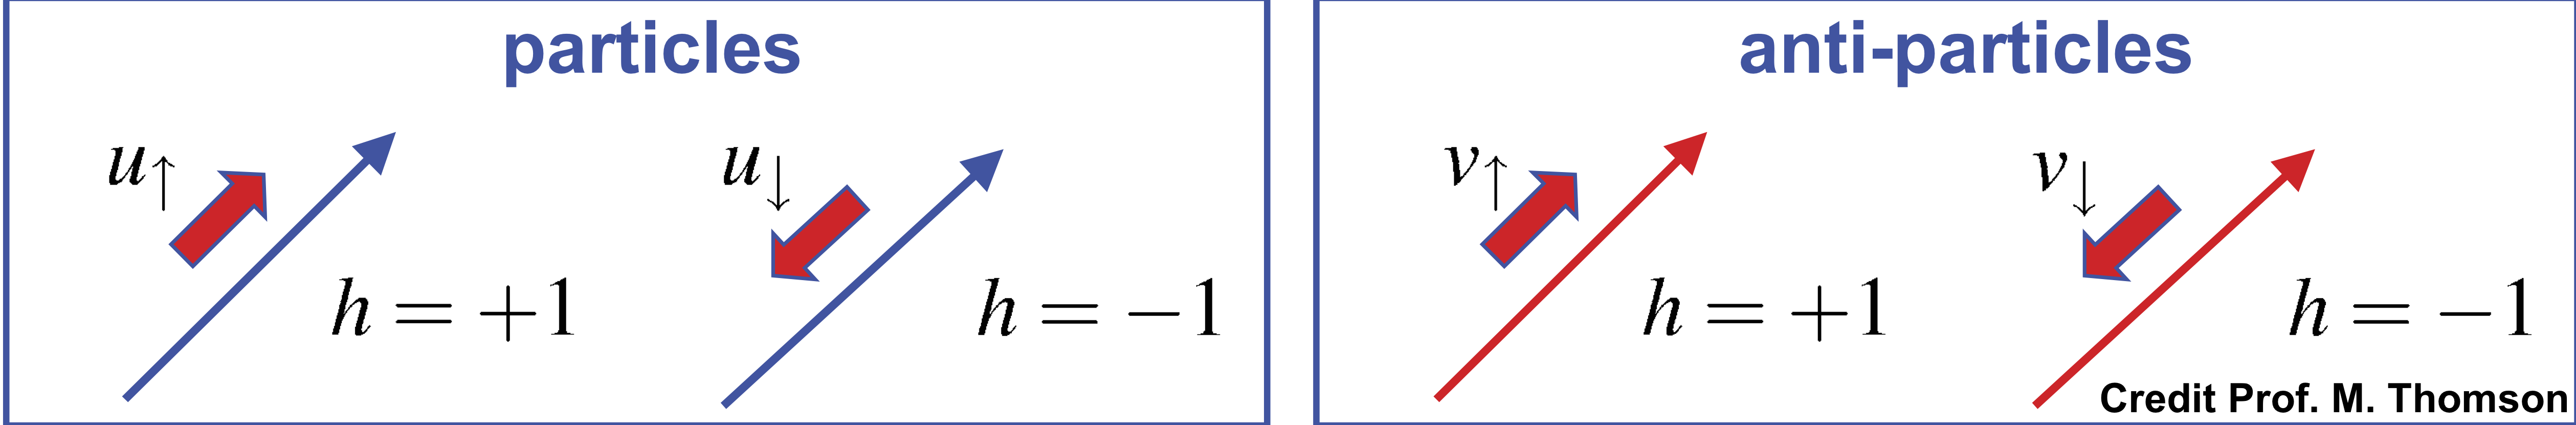
\includegraphics[width=0.97\textwidth]{fig/helicity.png}
\end{center}

\newpage

%% Week 4
\section{The strong force}

Question: What holds the nucleons (protons/neutrons) in a nucleus together?

\subsection{The early days: the Yukawa particle}

Based on the fact that the force holding nucleons together must be short range, as nucleons can be observed as free particles, without necessarily bonding into a nucleus, Hideki Yukawa in the 1930's (before the advent of Quantum Chromodynamics-QCD) suggested that the force holding nucleons together must be short range. {\bf Carrier of the strong force must be massive}, following the argument of Sec.~\ref{sec:massive_field}.

We can get an idea of what the mass of this force carrier should be by
considering that this carrier borrows some amount of energy $\Delta E$ (which is ok as long as it is paid back in time $\Delta t$ according to $\Delta E\Delta t\geq\hbar/2$) and traverses a distance $r_0$ determined by the size of a nucleon (the carrier needs to be exchanged between two nucleons in a nucleus).

We therefore have 
\[\Delta E\Delta t\sim\hbar/2,\]
\[\Delta t \sim\frac{r_0}{c},\] 
and \[\Delta E\sim m_{c}c^2.\]
Therefore for a nucleon size of $r_0\sim 10^{-15}$~m we can solve for $m_c$
yielding \[m_c=\frac{\hbar}{2r_0c}\sim 200m_e\sim \frac{1}{10}m_p\sim100~{\rm MeV}\]\footnote{This is just a dimensionality argument as you can see we have assumed a massive object travels at the speed of light...}
The fact that the mass of this carrier ($m_c$) is between the mass of a proton and the mass of the electron, it was named a meson (meaning in between).

\subsection{Discovery of the Yukawa meson}
\begin{figure}
\caption{Cecil Frank Powell}
\begin{tabular}{cc}
\parbox{0.32\textwidth}{
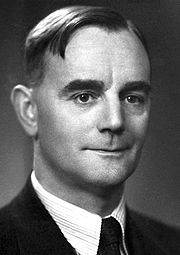
\includegraphics[width=0.3\textwidth]{fig/strongforce/180px-Cecil_Powell.jpg}
}&
\parbox{0.66\textwidth}{\textsf{\small
    ``Cecil Frank Powell took up a post in 1928 as Research Assistant to A.M. Tyndall in the H.H. Wills Physical Laboratory at the University of Bristol, later being appointed lecturer, and in 1948 appointed Melville Wills Professor of Physics. He was awarded the Nobel Prize in Physics for his development of the photographic method of studying nuclear processes and for the resulting discovery of the pion.'' 
}}
\end{tabular}
\\  \textsf{Source: \httplink{https://en.wikipedia.org/wiki/C.\_F.\_Powell}}
\end{figure}

In 1947 our very own Cecil Powell discovered a particle with a mass compatible to the mass of the Yukawa meson by measuring the traces that cosmic rays left in emulsion films on tops of mountains and air balloons. This Yukawa meson was called the Pion! He was awarded the Nobel Prize in 1969 for this discovery and the development of the photographic method for studying nuclear processes.
The principle of emulsion detection is very similar to that of a photographic film, offering high position resolution. A charged particle passing through the emulsion ionises atomic electrons of the emulsion. These electrons get trapped at a lattice defect at the surface of a crystal which makes up the emulsion. The trapped electrons in turn cause a chemical reaction which results in the development of (silver) filaments which manifest themselves as a dark spot on the emulsion.
\begin{figure}[!h]
\label{fig:pion_emulsion}
\begin{center}
\caption{Pion track captured in a photographic emulsion exposed to cosmic radiation. Pion enters the emulsion plate on the left of the image (track A) and undergoes multiple small angle scatters, loosing energy until it is captured by a nucleus which then disintegrates into proton tracks B,C,D. The top figure is a picture of the actual emulsion plate. The bottom figure is a trace of the star-shaped tracks on the right hand side of the top image. \textsf{Source: Nature 159 (1947)}.}
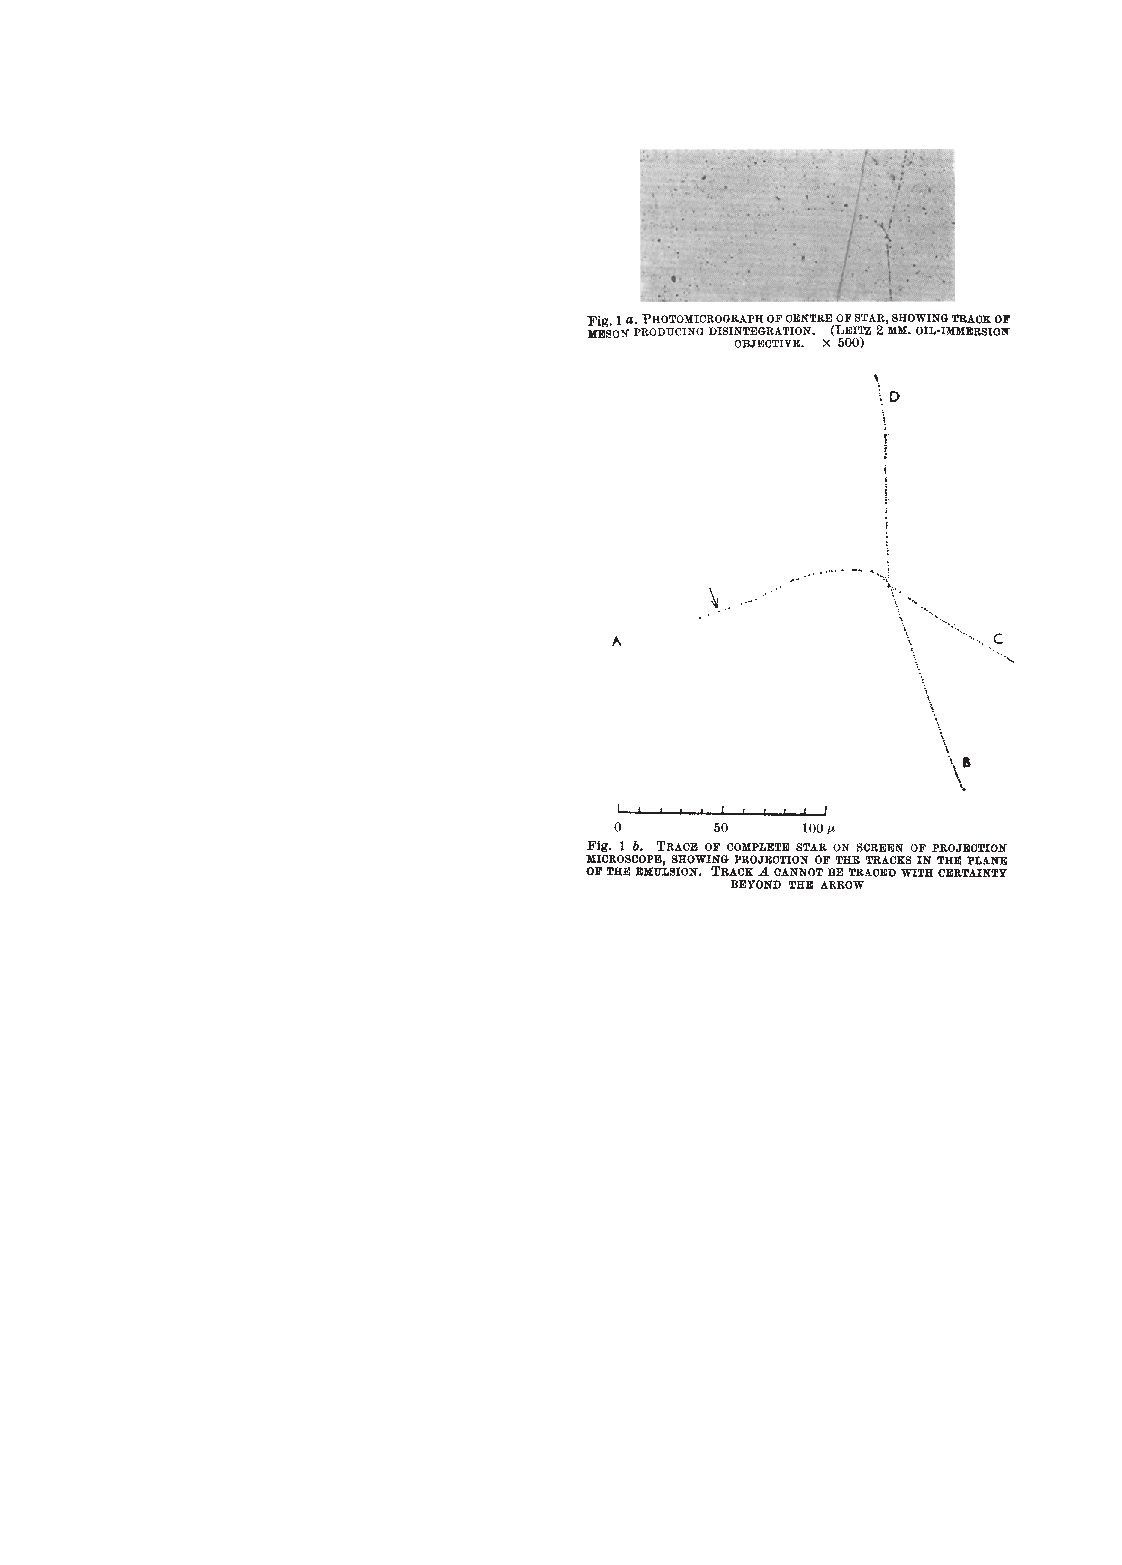
\includegraphics[width=0.80\textwidth]{fig/strongforce/pion_emulsion.pdf}
\end{center}
\end{figure}
By measuring the density of dots the pion left in the emulsion, as shown in Fig.~\ref{fig:pion_emulsion}, the angles at which the pion track scattered as it travelled through the emulsion, and the range the pion travelled before decaying, Powell was able to show that the mass of the pion was compatible to the mass of the Yukawa meson. In order to understand however how he could make such a measurement we need to understand how particles interact with matter.
\clearpage


\subsection{Consequences of the $\pi$-meson discovery}
\label{sec:isospinProtonsNeutronsPions}

\paragraph{It all made sense:} With the discovery of the pion it seemed that
strong interactions where completely understood. The nucleus is made up of proton and neutrons held together by a force mediated by the pion with a compling strength far larger ($\times 100$) in order to overcome the charge repulsion betwen the protons and hold the nucleus together.

Various scattering experiments between $p$ and $n$ as well as the binding energy of deuteron revealed that:
\begin{enumerate}
\item $m_p\sim m_n$
\item elastic scattering of protons and neutrons such as: 
\begin{center}
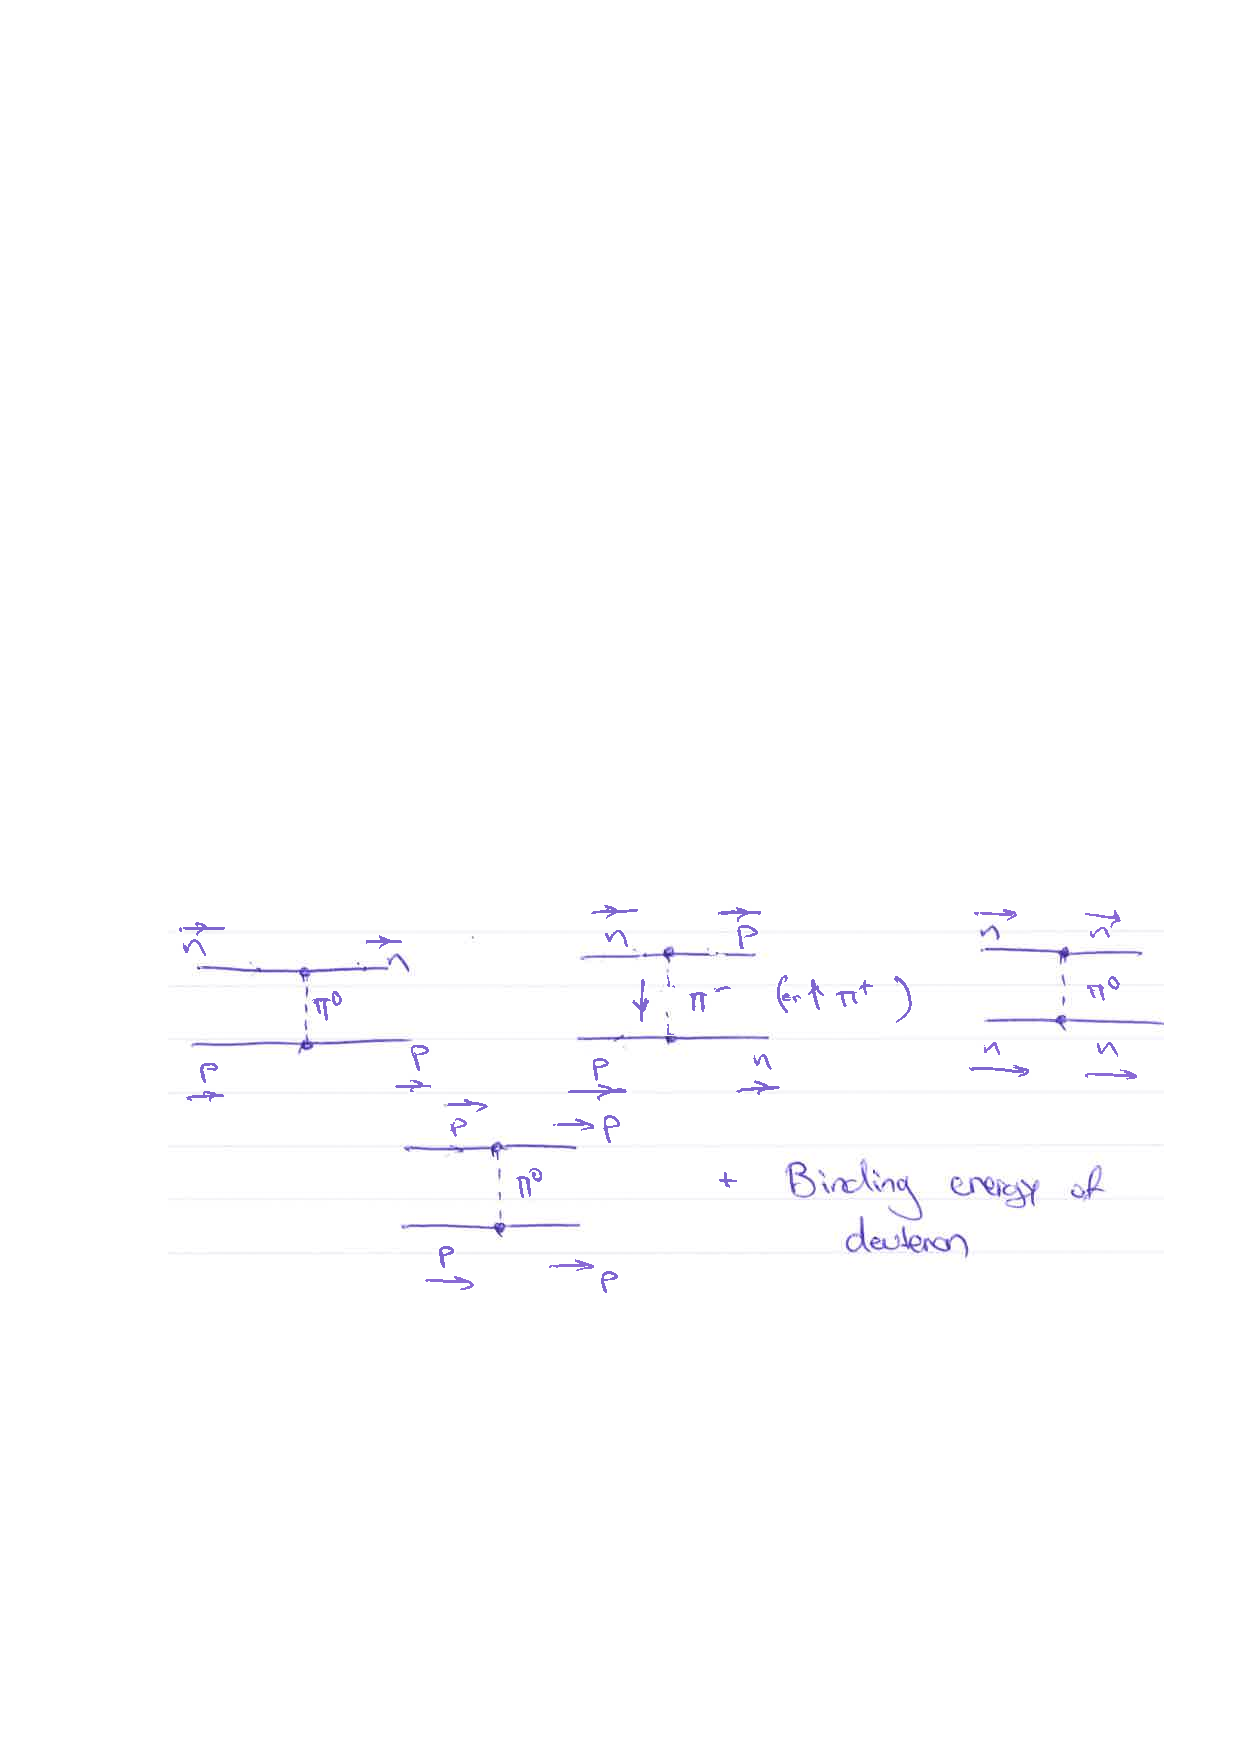
\includegraphics[width=0.98\textwidth]{fig/strongforce/proton_neutron_scattering.pdf}
\end{center}
all have same coupling strengths and must therefore have 3 different $\pi$-meson mediators with charges $0$, $+$ and $-$.
\end{enumerate}
The above two points means that the Strong force acts the same if in a process involving neutrons and or protons, you swap the neutrons with protons and vice versa.

Heisenberg in 1932 suggested that the neutron and the proton are considered as different states of a single entity ``the Nucleon'', in complete analogy to an electron which has two spin states: spin-up and spin-down. He therefore called this new quantum number Strong-Isospin.

For $n$ and $p$ which form an Isospin-Doublet: $I_s=\frac{1}{2}$ with $I_{s3}=\pm\frac{1}{2}$. Conventionally $I_{s3}^{p}=+\frac{1}{2}$ and $I_{s3}^{n}=-\frac{1}{2}$. 

Similarly, $\pi^+$, $\pi^-$ and $\pi^0$ mesons form an Isospin-Triplet with 
$I_{s}=1$, $I_{s3}^{\pi^+}=+1$, $I_{s3}^{\pi^0}=0$, $I_{s3}^{\pi^-}=-1$.

Points 1 and 2 suggest that the strong isospin operator $\hat{I_s}$ commutes with the hamiltonian
of the strong interactions $\hat{H_{s}}$. This in turn means that strong isospin is conserved in strong interaction. This means that under a strong interaction, the strong isospin of an initial state must be the same as strong isospin of the final state. Lets take a look at some reactions:

\paragraph{Examples}: 
\begin{itemize}
\item Consider the process $pp\to d\pi^+$ where $d$ is a Deuteron. The deuteron carries $I_s=0$ and $I_{s3}=0$. Using Dirac notation to denote the strong isospin states ($|I_s,I_{s3}>$), the initial state is a combination of two $|1/2,1/2>$ states, ie
\[
{\rm Initial:}~|1/2,1/2>|1/2,1/2>=|1,1>\\
\]
In contrast the final state is a combination of a $|0,0>$ and $|1,1>$ states, ie
\[
{\rm Final:}~|0,0>|1,1>=|1,1>
\]

Note that we have used the principles of quantum mechanical angular momentum addition to determine the total isospin of the initial and final states. Remember: 
\[
|I_{s}^{(1)}-I_{s}^{(2)}|\leq I_{s}^{tot}\leq I_{s}^{(1)}+I_{s}^{(2)}
\]
\[
I_{s3}^{tot}=I_{s3}^{(1)}+I_{s3}^{(2)}
\]
So combining two $|1/2,1/2>$ states gives us $|1,1>$. In contrast, combining a $|0,0>$ with a $|1,1>$ state gives us a $|1,1>$ state. So in this process the total strong isospin of the initial and final states is the same and therefore the process conserves strong isospin and is therefore allowed.

\item Consider the process $pn\to d\pi^0$. The initial state is a combination of a $|1/2,1/2>$ and $|1/2,-1/2>$ states, ie
\[
{\rm Initial:}~|1/2,1/2>|1/2,-1/2>=\sqrt{\frac{1}{2}}(|1,0>+|0,0>).\\
\]
In contrast the final state is a combination of a $|0,0>$ and $|1,0>$ states, ie
\[
{\rm Final:}~|0,0>|1,0>=|1,0>
\]
Note that we have again used the principles of quantum mechanical angular momentum addition
to determine the total isospin of the initial and final states.

We also make use of the Clebsch-Gordan coefficients to determine the exact mixture
of total isospin states. Don't worry if you have never seen this. We will give
you the expressions for the total isospin states anyway. Lets explain a bit in detail how we reached this result:

So combining  states $|1/2,1/2>$ and $|1/2,-1/2>$, 
results in $I_{s}^{tot}=0$ or $I_{s}^{tot}=1$ with $I_{s3}^{tot}=0$. The Clebsh-Gordan table tells us that we can therefore write: $|1/2,1/2>|1/2,-1/2>=\sqrt{\frac{1}{2}}(|1,0>+|0,0>)$.

However combining states $|0,0>|1,0>$ results in only one option, $I_{s}^{tot}=1$ with $I_{s3}^{tot}=0$.

Ok so how does strong isospin conservation fit into all this? Well the final state is $|1,0>$, therefore since isospin is conserved, only $pn$ states in a $|1,0>$ and NOT in a $|0,0>$ can decay to a $d\pi^0$ state. This means that in contrast to the previous example, where both initial and final states are found in a single configuration, the process $pn\to d\pi^0$ occurs at a lower rate by a factor of $\sqrt{\frac{1}{2}}^2=\frac{1}{2}$ compared to $pp\to d\pi^+$.
This is because the initial $pn$ state must be in a $|1,0>$ in order to decay via the strong interaction to $d\pi^0$ which is also a $|1,0>$ state. The probability of the $pn$ state to be in a $|1,0>$ configuration is given by the square of the coefficient in front of the $|1,0>$ term ie
$\sqrt{\frac{1}{2}}^2$.
\item The $\rho^0$ meson is an excited state of the $\pi^0$ meson. It has a strong isospin state of $|1,0>$. The $\rho^0$ decays primarily to a $\pi^+$ and a $\pi^-$ but never to a pair of $\pi^0$ mesons. One of the reasons is because the decay of the $\rho^0$ primarily occurs through the strong force so isospin must be conserved. Lets consider the isospin configurations of the two final states (consulting the Clebcsh-Gordan table):
\[
\pi^0\pi^0: |1,0>|1,0> =\sqrt{\frac{2}{3}}|2,0>+0|1,0>-\sqrt{\frac{1}{3}}|0,0>
\]
\[
\pi^+\pi^-: |1,1>|1,-1> =\sqrt{\frac{1}{6}}|2,0>+\sqrt{\frac{1}{2}}|1,0>+\sqrt{\frac{1}{3}}|0,0>
\]
Therefore as you can see the factor in front of the $|1,0>$ state which corresponds to the strong isospin state of the $\rho^0$ is 0! This means that 2 $\pi^0$ mesons can never be in a strong isospin configuration required by the $\rho^0$, in contrast to the $\pi^+\pi^-$ state which can. This means that the $\rho^0$ CAN decay via the strong force to $\pi^+\pi^-$ but CANNOT decay to  $\pi^0\pi^0$\footnote{You will see later that $\rho^0\to\pi^0\pi^0$ also violates another symmetry of both the strong and electromagnetic interactions: Charge-conjugation symmetry.}.

\end{itemize}

\subsection{Extending Strong-Isospin to the quark sector and the existence of colour}
\label{sec:isospinQuarks}
The proton is made up of 2 up-type quarks and 1 down-type quark (uud).
The neutron is made up of 1 up-type quark and 2 down-type quarks (udd).
We can extend the idea that the strong force treats neutrons and protons equally,
to treating up-type and down-type quarks equally. 

So as we did before, we consider the up and down quarks as different states of a single
entity. The strong isospin of the up-quark has $I_{s}=\frac{1}{2}$ with 
$I_{s3}=+\frac{1}{2}$ and the down-quark has $I_{s}=\frac{1}{2}$ with $I_{s3}=-\frac{1}{2}$.
We can therefore use the principles behind angular momentum addition, to construct the total isospin of the proton, neutron and other quark bound states. 

So combining three quarks of two isospin states (or quark flavours $u=|\frac{1}{2},+\frac{1}{2}>$ and $d=|\frac{1}{2},-\frac{1}{2}>$) we get
eight states: $uuu,~uud,~udu,~udd,~duu,~dud,~ddu,~ddd$ with total isospin:
\begin{center}
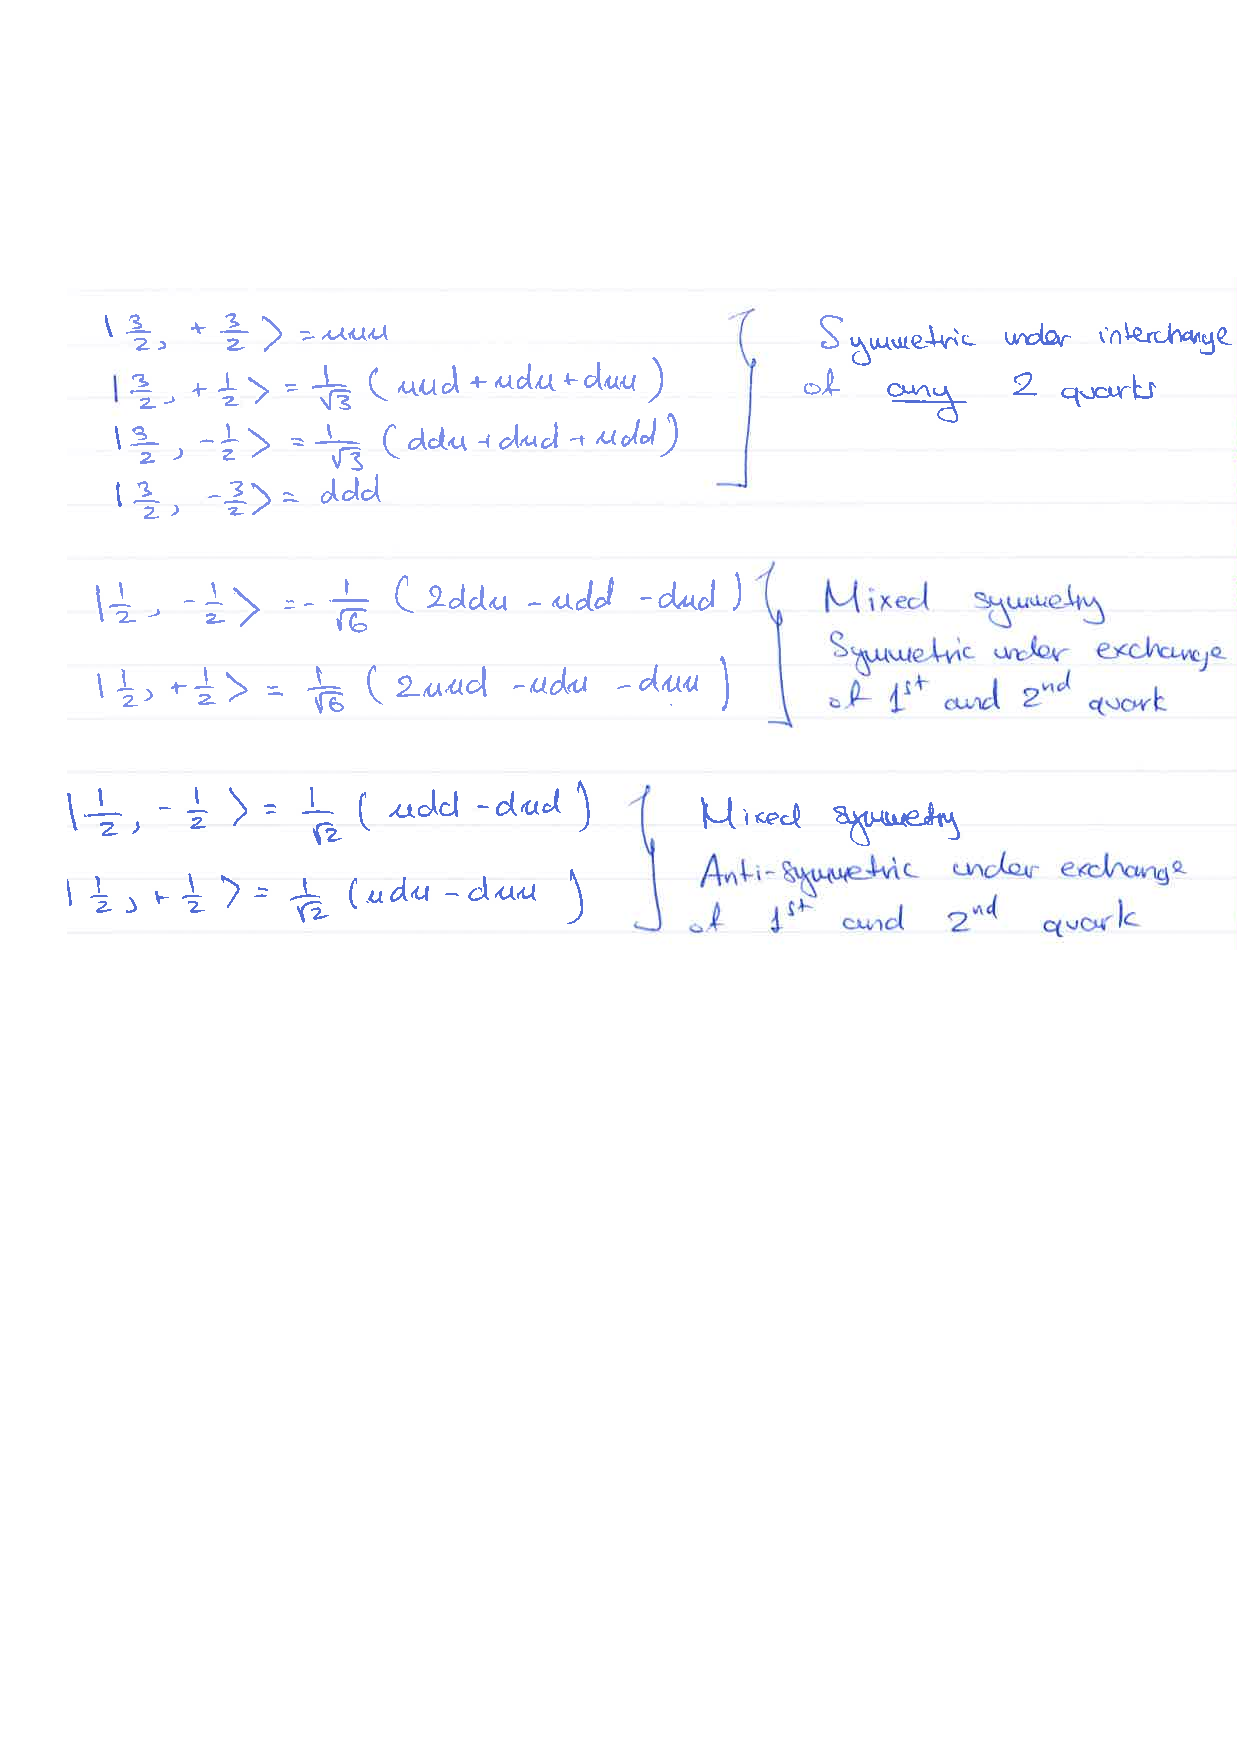
\includegraphics[width=0.98\textwidth]{fig/strongforce/baryon_isospin.pdf}
\end{center}
Ok so why stop here. Lets play the same game with the spin of this three-quark system. Remember quarks are fermions, they obey the Dirac equation and therefore carry spin $S=\frac{1}{2}$ and $S_3=\pm\frac{1}{2}$. So just like with isospin, we have eight spin states:
\begin{center}
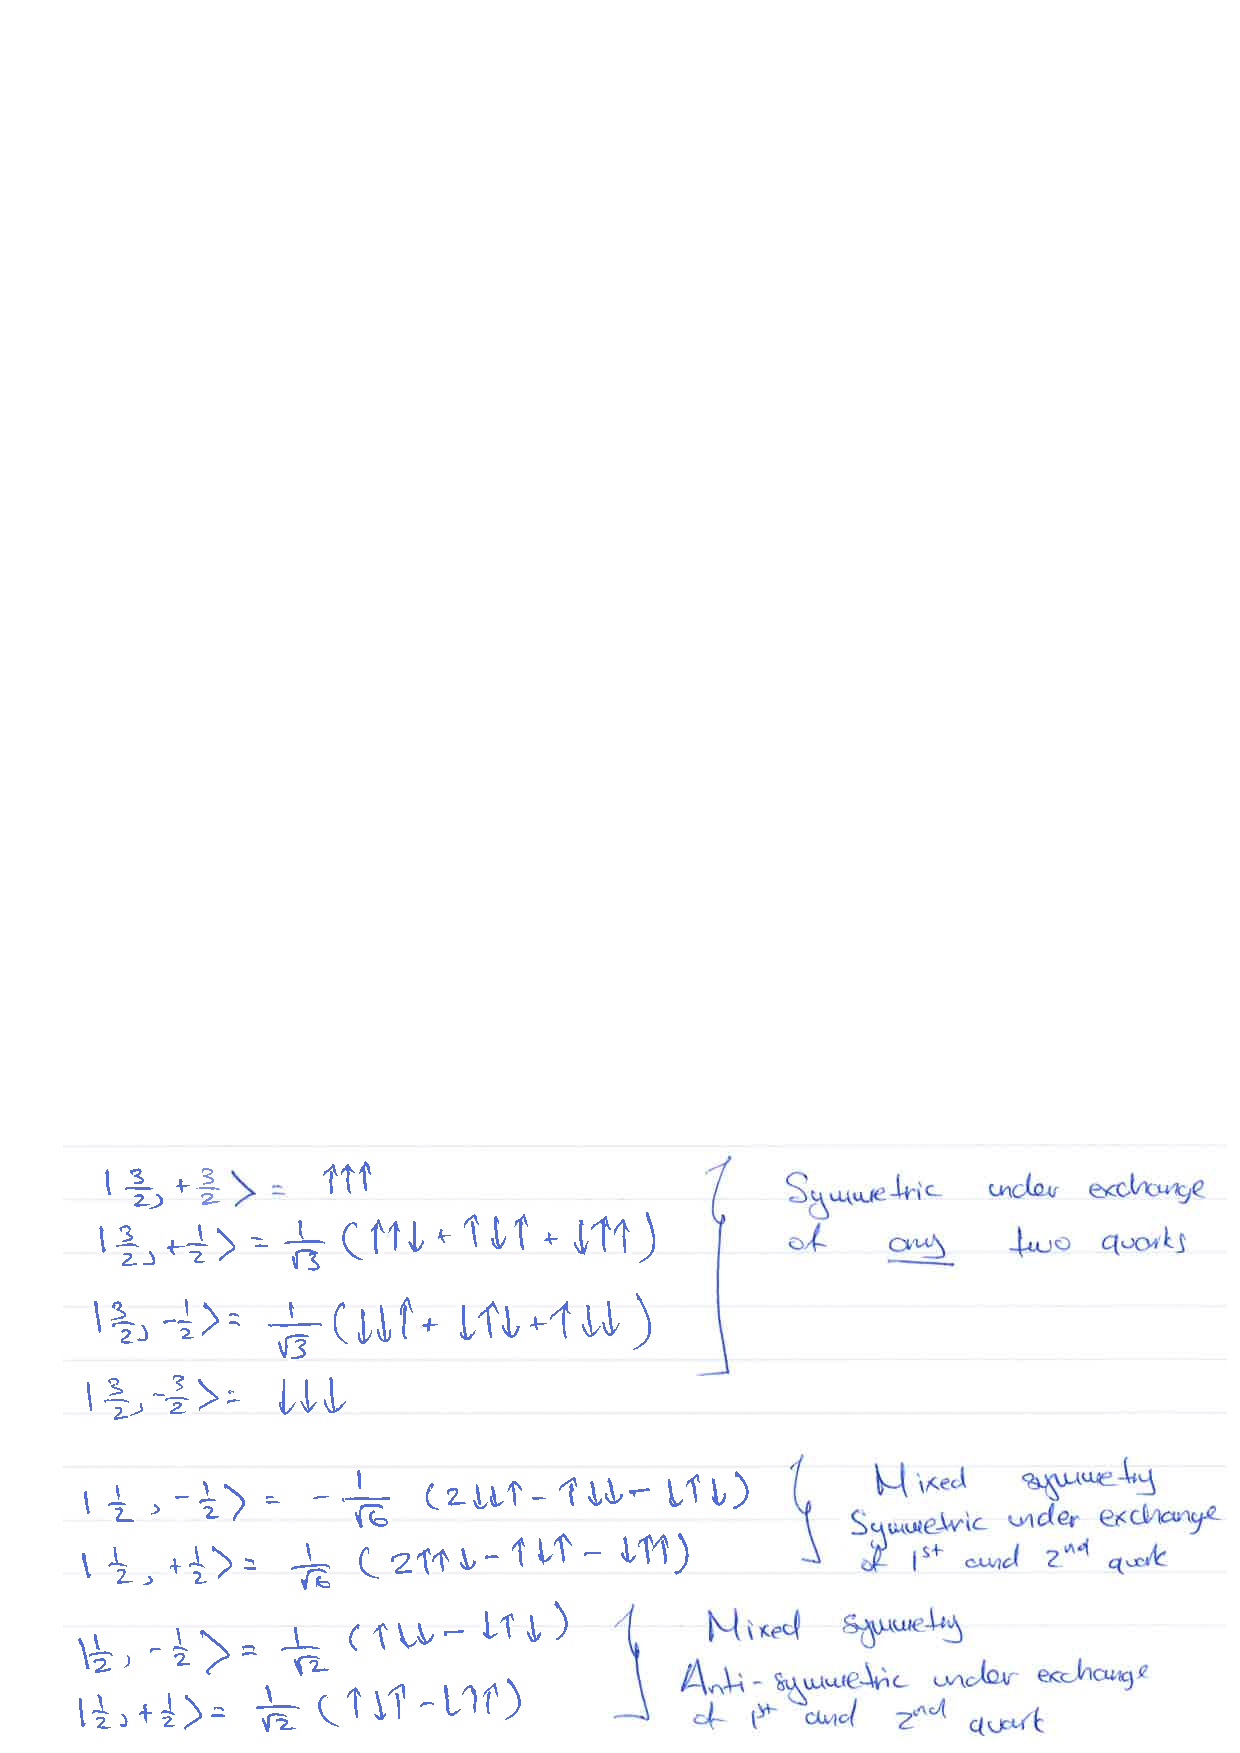
\includegraphics[width=0.98\textwidth]{fig/strongforce/baryon_spin.pdf}
\end{center}

So far we have considered two parts of the total wave-function of a bound state of 3 quarks (known as a Baryon). There is an additional part of the wave-function relating to the spatial part of the 3-quark combination. Putting all this together we have
\begin{equation}
\label{eq:psi_total_no_colour}
\psi_{\rm total}=\phi_{\rm isospin}\chi_{\rm spin}\eta_{\rm space}.
\end{equation}

Now given that baryons are made of up 3 quarks (fermions) there is another aspect we need to consider. The Pauli exclusion principle states that no two electrons (also fermions) can occupy the same quantum number state. This principle was devised in order to be able to explain why atomic electrons don't all cascade down to the ground state. This might sound somewhat ad-hoc however the Pauli principle is rooted on something deeper. 

{\bf The wave function of indistinguishable fermions must be anti-symmetric under the exchange of any two fermions.}
This means that for a wave function made up of two particles $\psi(1,2)$, must satisfy $\psi(1,2)=-\psi(2,1)$.

For example, consider one fermion in state $\psi_\alpha$ and a second fermion in state $\psi_\beta$. The total wave function is $\psi(1,2)=\psi_\alpha(1)\psi_\beta(2)$.
However, since the fermions are indistinguishable, the state  $\psi(1,2)=\psi_\alpha(2)\psi_\beta(1)$ is indistinguishable from the previous one. Thus both of these
wavefunctions describe the same state so we need to take the superposition of them. Since we require that $\psi(1,2)=-\psi(2,1)$, we can write $\psi(1,2)$ as
\footnote{Similarly, indistinguishable bosons would satisfy
$\psi(1,2)=\frac{1}{\sqrt{2}}[ \psi_\alpha(1)\psi_\beta(2)+\psi_\alpha(2)\psi_\beta(1)]$.
}
\[
\psi(1,2)=\frac{1}{\sqrt{2}}[ \psi_\alpha(1)\psi_\beta(2)-\psi_\alpha(2)\psi_\beta(1) ].
\]
We can now see Pauli's exclusion principle in action. If both fermions $1$ and $2$ where in the same state $\alpha$, then  $\psi(1,2)=0$.

Coming back to Eq.~\ref{eq:psi_total_no_colour}, from what we have learnt, $\psi_{\rm total}$ of the baryon must be antisymmetric under the exchange of any pair of quarks. For what follows let us consider only ground state baryons, that is baryons withe orbital angular momentum $L=0$. In this case, $\eta_{\space}$ is totally symmetric. This means that the product $\phi_{\rm isospin}\chi_{\rm spin}$ must be totally anti-symmetric. This in turn would mean that the state
\[
(uuu)(\uparrow\uparrow\uparrow)=|(\frac{3}{2},+\frac{3}{2})_{\rm isospin},(\frac{3}{2},+\frac{3}{2})_{\rm spin}>
\]
should not be a physical state as it is totally-symmetric. However in scattering
experiments of a $\pion$ beam off a proton target, a charge +2 particle was observed, the $\Delta^{++}$ compatible with a $(uuu)(\uparrow\uparrow\uparrow)$ state.



{\bf Therefore something is missing in Eq.~\ref{eq:psi_total_no_colour}. The missing ingredient is colour charge!}

In order to explain the observed pattern of baryons, their masses and spins another component to the wave-function of the baryon was required. The colour wave-function. Equation~\ref{eq:psi_total_no_colour} is then modified to
\begin{equation}
\label{eq:psi_total_colour}
\psi_{\rm total}=\phi_{\rm isospin}\chi_{\rm spin}\eta_{\rm space}\zeta_{\rm colour}.
\end{equation}
where $\zeta_{\rm colour}$ is antisymmetric under the exchange of any 2 quarks. 
The only completely anti-symmetric state has a net colour quantum number of 0.
{\bf All baryons and mesons have a net colour charge of 0}. 
So with our friend the $\Delta^{++}$, the requirement that $\zeta_{\rm colour}$ is totally antisymmetric, means that $\phi_{\rm isospin}\chi_{\rm spin}$ must be totally symmetric for ground state baryons.

\paragraph{Mesons:} Note that so far our focus has been on three quark bound states (baryons). We can follow a similar treatment of bound states of a quark and anti-quark (mesons) like the $\pi^+$ which is a $u\bar{d}$ state. Constructing the meson wave-function does not suffer from the complication that the overall wavefunction has to be anti-symmetric as we are dealing with distinguishable fermion anti-fermion states.

\paragraph{The strange quark:}
The discovery of strange hadrons (hadrons containing strange quarks) in cosmic rays such as the $K^+$ meson (a bound state between $u\bar{s}$) requires to add to the previous picture a new quantum number called strangeness. Strangeness is conserved in strong interactions but not in weak interactions. This is because the strange quark can decay to another quark through the weak interaction, as you will see later in the course. We know that the mass of the strange quark is not the same as the mass of the $u$ and $d$ quarks, however the mass 
difference between baryons that contain a strange quark is small compared to the total baryon mass. For example the $\Lambda^{0} (uds)$ has a mass of 1.1~GeV and the $n(udd)$  has a mass of 0.9~GeV. We can therefore say that the strong force is approximately symmetric under the exchange of a $u$ or $d$ quark, with an $s$ quark. We can refer to this symmetry as ``Flavour Symmetry''.
So we can repeat the above exercise where we extend strong-isospin of quarks to include the strange quark, that is we identify
$u=|1,+1>,s=|1,0>,d=|1,-1>$. 

\paragraph{Putting it all together:}
The plethora of hadronic states discovered during the 40s 50s and 60s could be explained using the principles of flavour symmetry, fermi-statistics and a new quantum number ``colour''. Murray Gell-Mann constructed this model in 1961 which led to the development of the quark model. His model predicted the existence of a spin-3/2 $sss$ state with a mass near $1680$~MeV (the $\Omega^-$). A particle matching these properties was subsequently discovered in 1964 which earned Gell-Mann the Nobel Prize in 1969.

\begin{center}
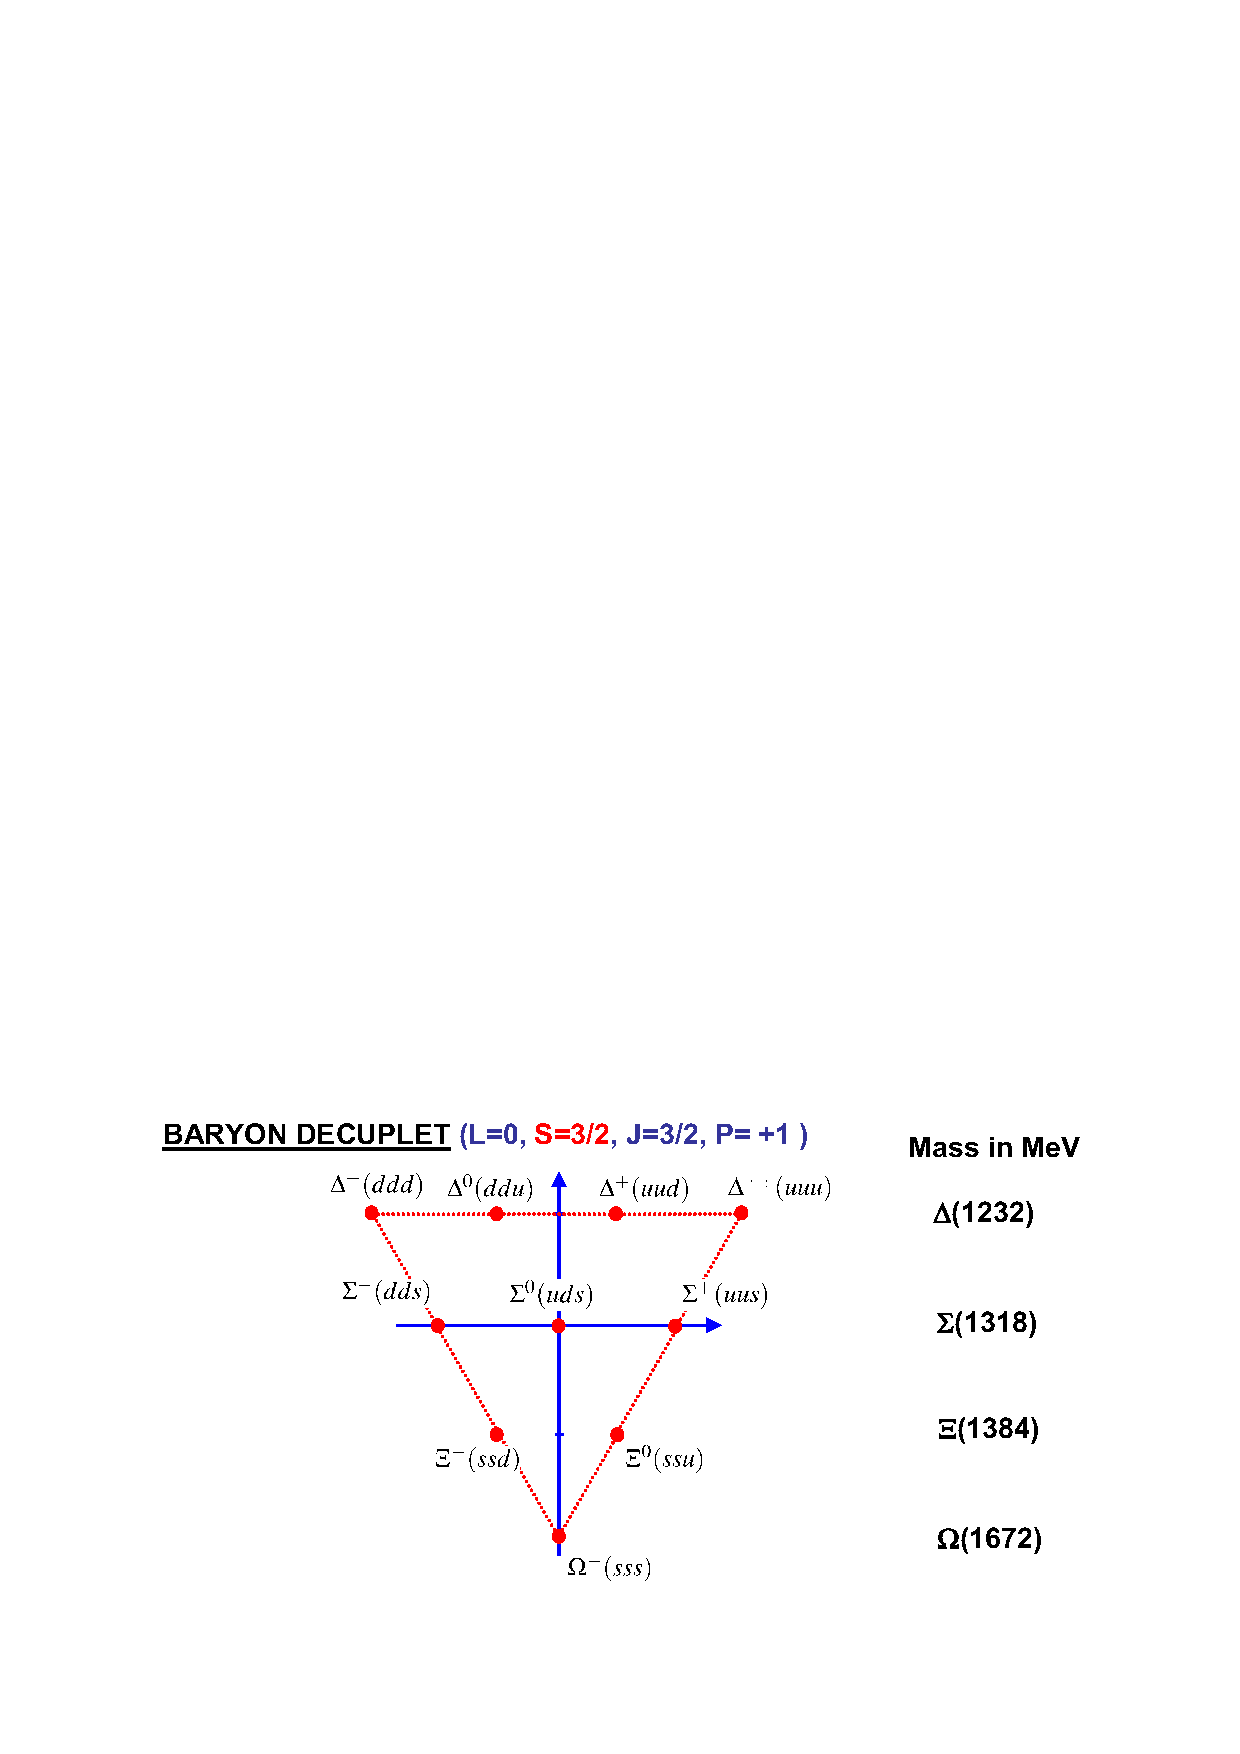
\includegraphics[width=0.65\textwidth]{fig/strongforce/baryon_decouplet.pdf}\\
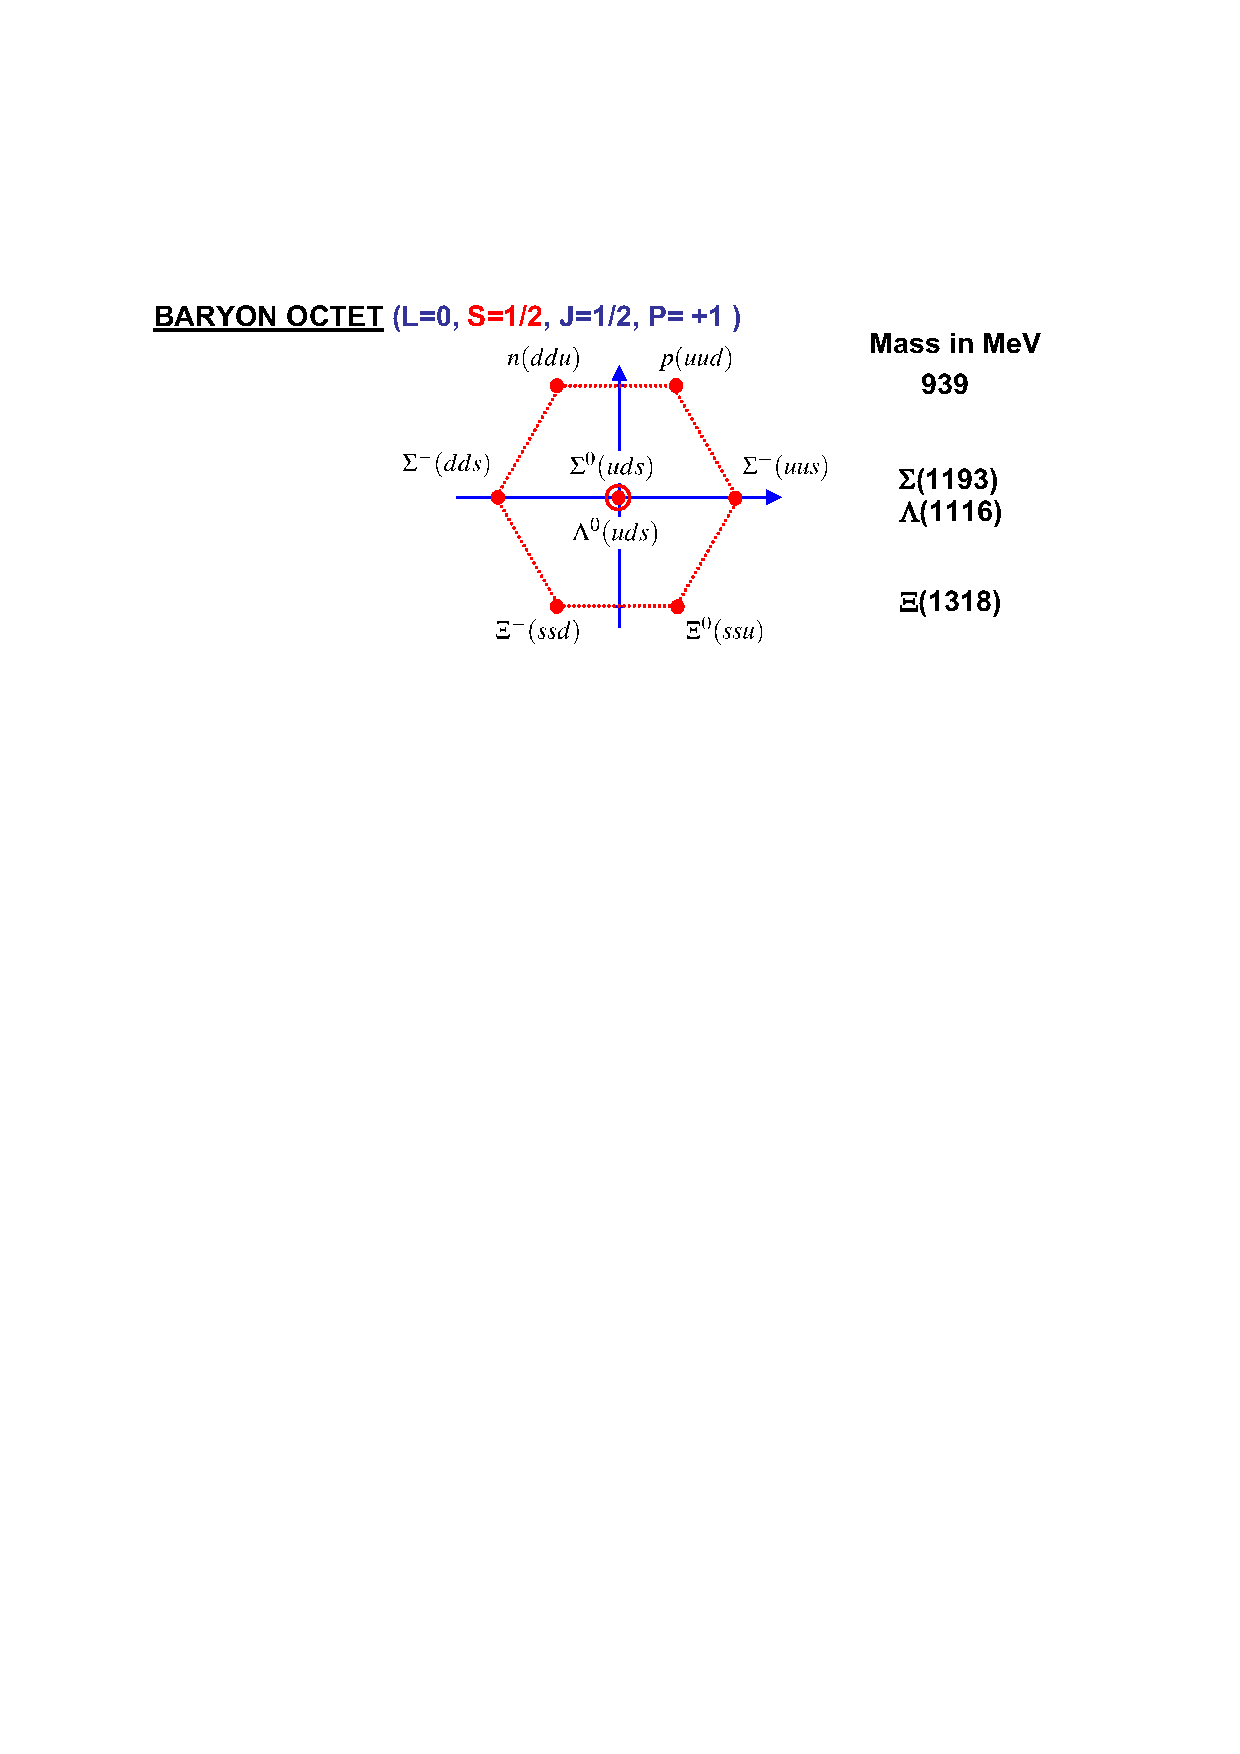
\includegraphics[width=0.7\textwidth]{fig/strongforce/baryon_octet.pdf}\\
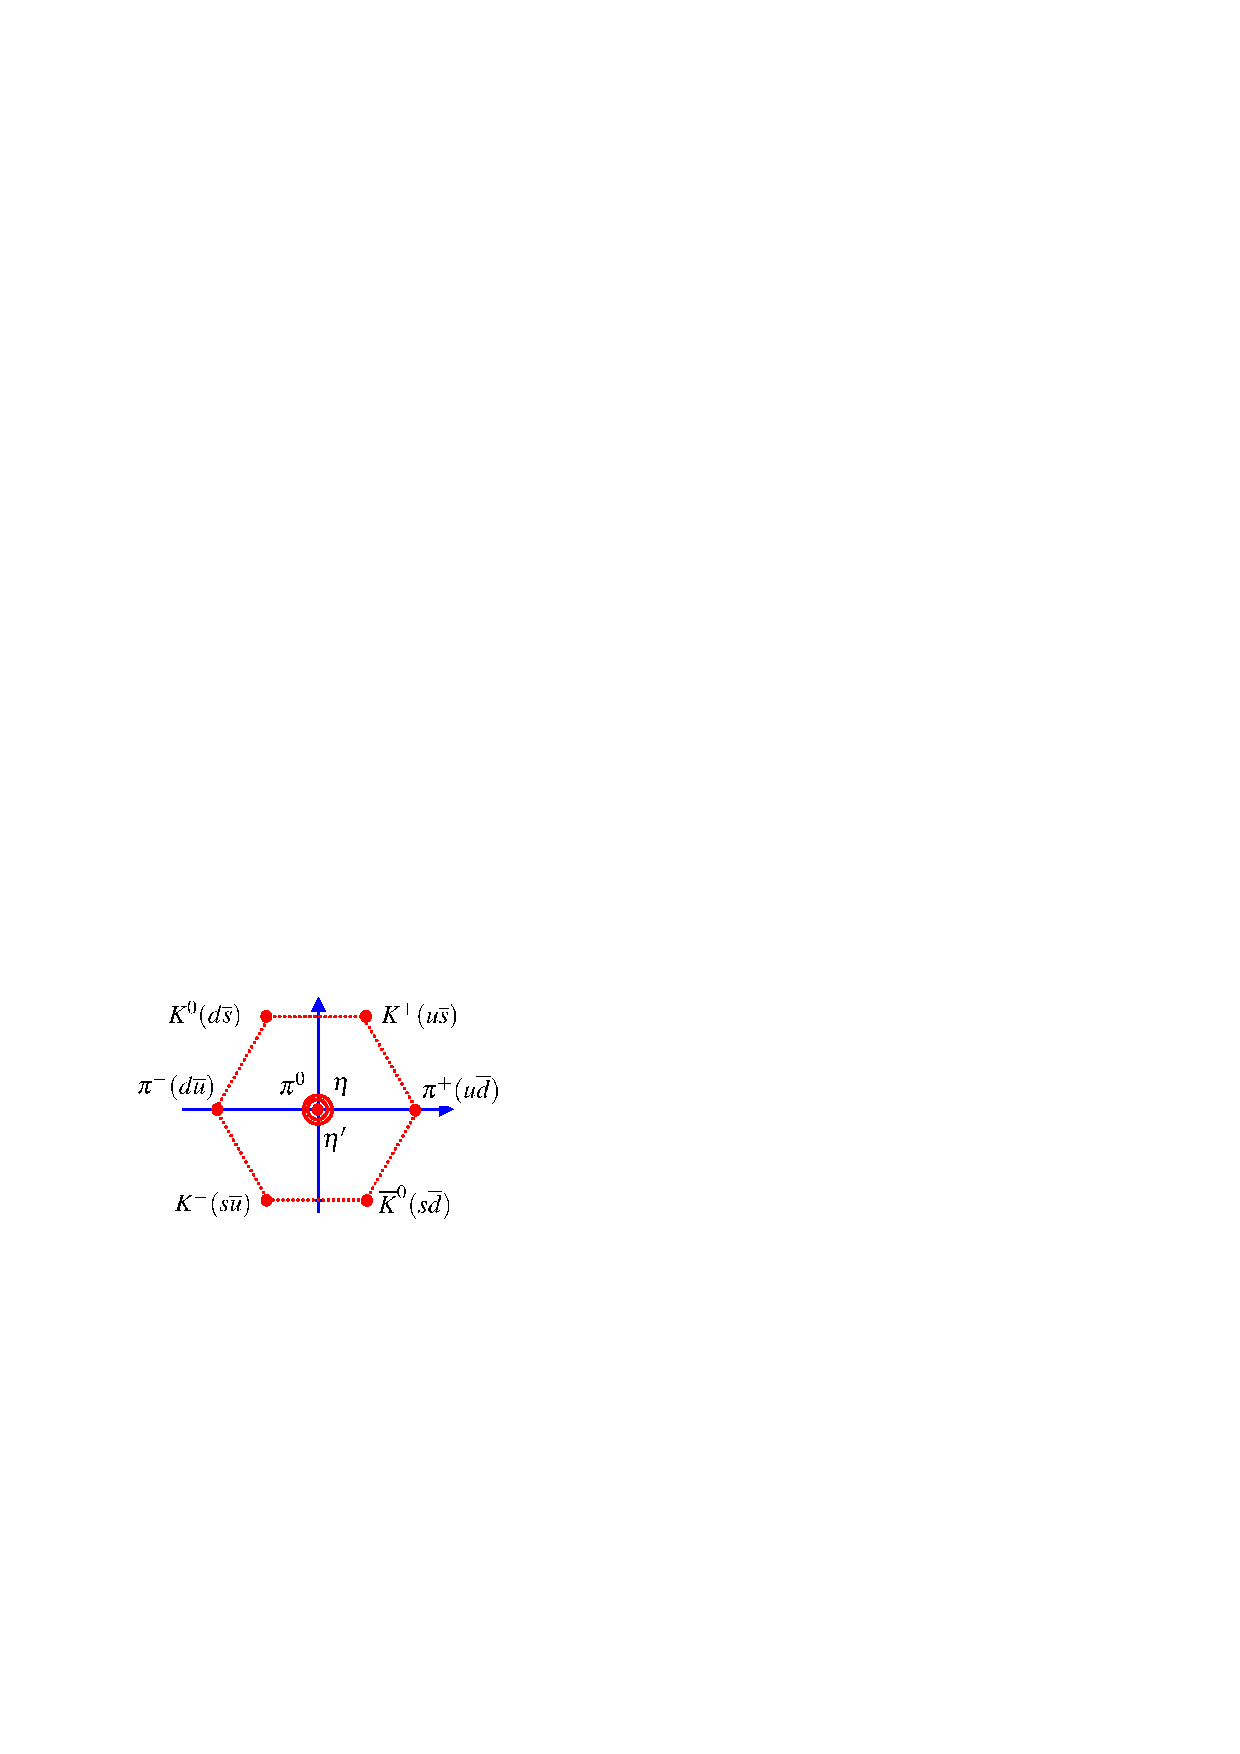
\includegraphics[width=0.4\textwidth]{fig/strongforce/scalar_mesons.pdf}\\
{\tiny Source: Prof. M. A. Thomson \httplink{http://www.hep.phy.cam.ac.uk/~thomson/lectures/partIIIparticles/Handout7\_2009.pdf}}
\end{center}
If flavour symmetry between the three quark types was exact, then all baryons and mesons would have exactly the same mass irrespective of how many strange quarks they contain.

\subsection{Colour Confinement}
We demonstrated that hadrons required an additional totally antisymmetric component to their wave-function. This was in order to explain the existence of the large number of observed baryons while still requiring that their overall wave-function is anti-symmetric under the exchange of any two quarks.

By requiring that each quark carries a new quantum number called ``colour'' (or ``colour charge'') we can construct a totally anti-symmetric wave function out of three quarks if the colour charge can have three values ``{\bf r}ed'', ``{\bf g}reen'', and ``{\bf b}lue''\footnote{You can see why you need three types of colour, because looking back at the symmetries of the spin part of the baryonic wave-function, you can see that you can never build a totally anti-symmetric wave function which is made up of 3 quarks and only two spin quantum numbers (spin-up, spin-down).}. Anti-quarks carry colour charges of ``anti-red'', ``anti-blue'', ``anti-green''.

In this case, there is a single such combination which also gives rise to a total colour charge of 0. For baryons this combination is:
\[
\zeta_{\rm colour}^{qqq}=\frac{1}{\sqrt{6}}(rgb-rbg+gbr-grb+brg-bgr)
\]
As discussed earlier, for mesons  there is no restriction that the wave function is antisymmetric as mesons are made up of distinguishable quarks and anti-quarks ($q\bar{q}$). However there seems to be a more fundamental principle that determines the colour wave-function of all hadrons and also restricts the types of bound states one could form out of quarks. This principle is known as ``colour confinement'', which states that:\\\\
{\bf Only states with a total colour charge of 0 can exist as free particles.}\\\\
There is no direct proof, other than all experimental evidence seems to point to this fact. This is the reason why the colour wave-function of mesons is given by:
\[
\zeta_{\rm colour}^{q\bar{q}}=\frac{1}{\sqrt{3}}(r\bar{r}+g\bar{g}+b\bar{b})
\]
which is has a total colour charge of 0. 

Additionally the above principle is also why we cannot form bound states of $qq\bar{q}$ or $qq$ quarks as we cannot obtain a colour-less state from these combination of quarks. However states like $q\bar{q}q\bar{q}$ and $qqqq\bar{q}$ are indeed allowed and the LHCb experiment (last July) seems to have some first hard evidence of the existence of such exotic states, as shown in Fig.~\ref{fig:lhcb_pentaquark}.
\begin{figure}
\centering
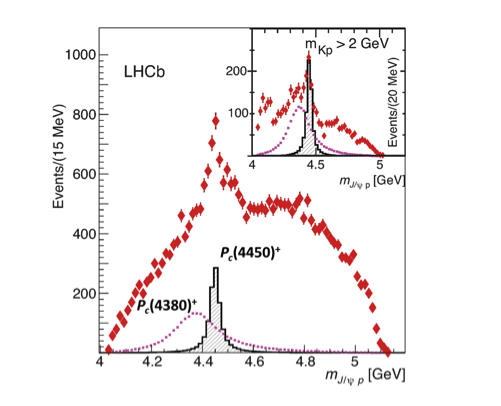
\includegraphics[width=0.65\textwidth]{fig/strongforce/lhcb_pentaquark.png}
\caption{The invariant mass between the proton ($p$) and the $J/\psi$ meson (a bound state of $c\bar{c}$ quarks) from the decay of a $\Lambda_{b}$ baryon (like a proton but with a $udb$ quark content) to a $J/\psi$, a proton and a $K^-$. The data are shown as red diamonds. The predicted distributions of the 5-quark bound states (penta-quarks) $P_c(4380)^+$ amd $P_c(4450)^+$ states are indicated in the purple and black distributions. The quark contents of these states are thought to be $uudc\bar{c}$.{\tiny Source:\httplink{http://press.web.cern.ch/press-releases/2015/07/cerns-lhcb-experiment-reports-observation-exotic-pentaquark-particles} and \httplink{http://arxiv.org/abs/1507.03414}}}
\label{fig:lhcb_pentaquark}
\end{figure}

\subsection{The role of the gluon in confinement}
Just like the EM charge, the strong charge is conserved at each vertex.
However, the fact that we have 3 types of colour charges for quarks, and 3 types
for anti-quarks means that the gluon, the massless carrier of the strong interaction, will also carry colour charge (in fact it carries one colour and one anti-colour charge). This is in contrast to EM interactions where the photon is electrically neutral.\footnote{For a formal proof of this effect take the 4th year course! If interested, it is because the gluon lies in the Lie algebra of an SU(3) group, compared to the photon which lies in the Lie algebra of a U(1) group}
\begin{center}
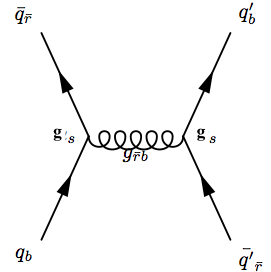
\includegraphics[width=0.5\textwidth]{fig/strongforce/gluon_qqbar.png}
\end{center}

The fact that the gluon now carries colour charge means that it can interact with itself so we have vertices of the type:
\begin{center}
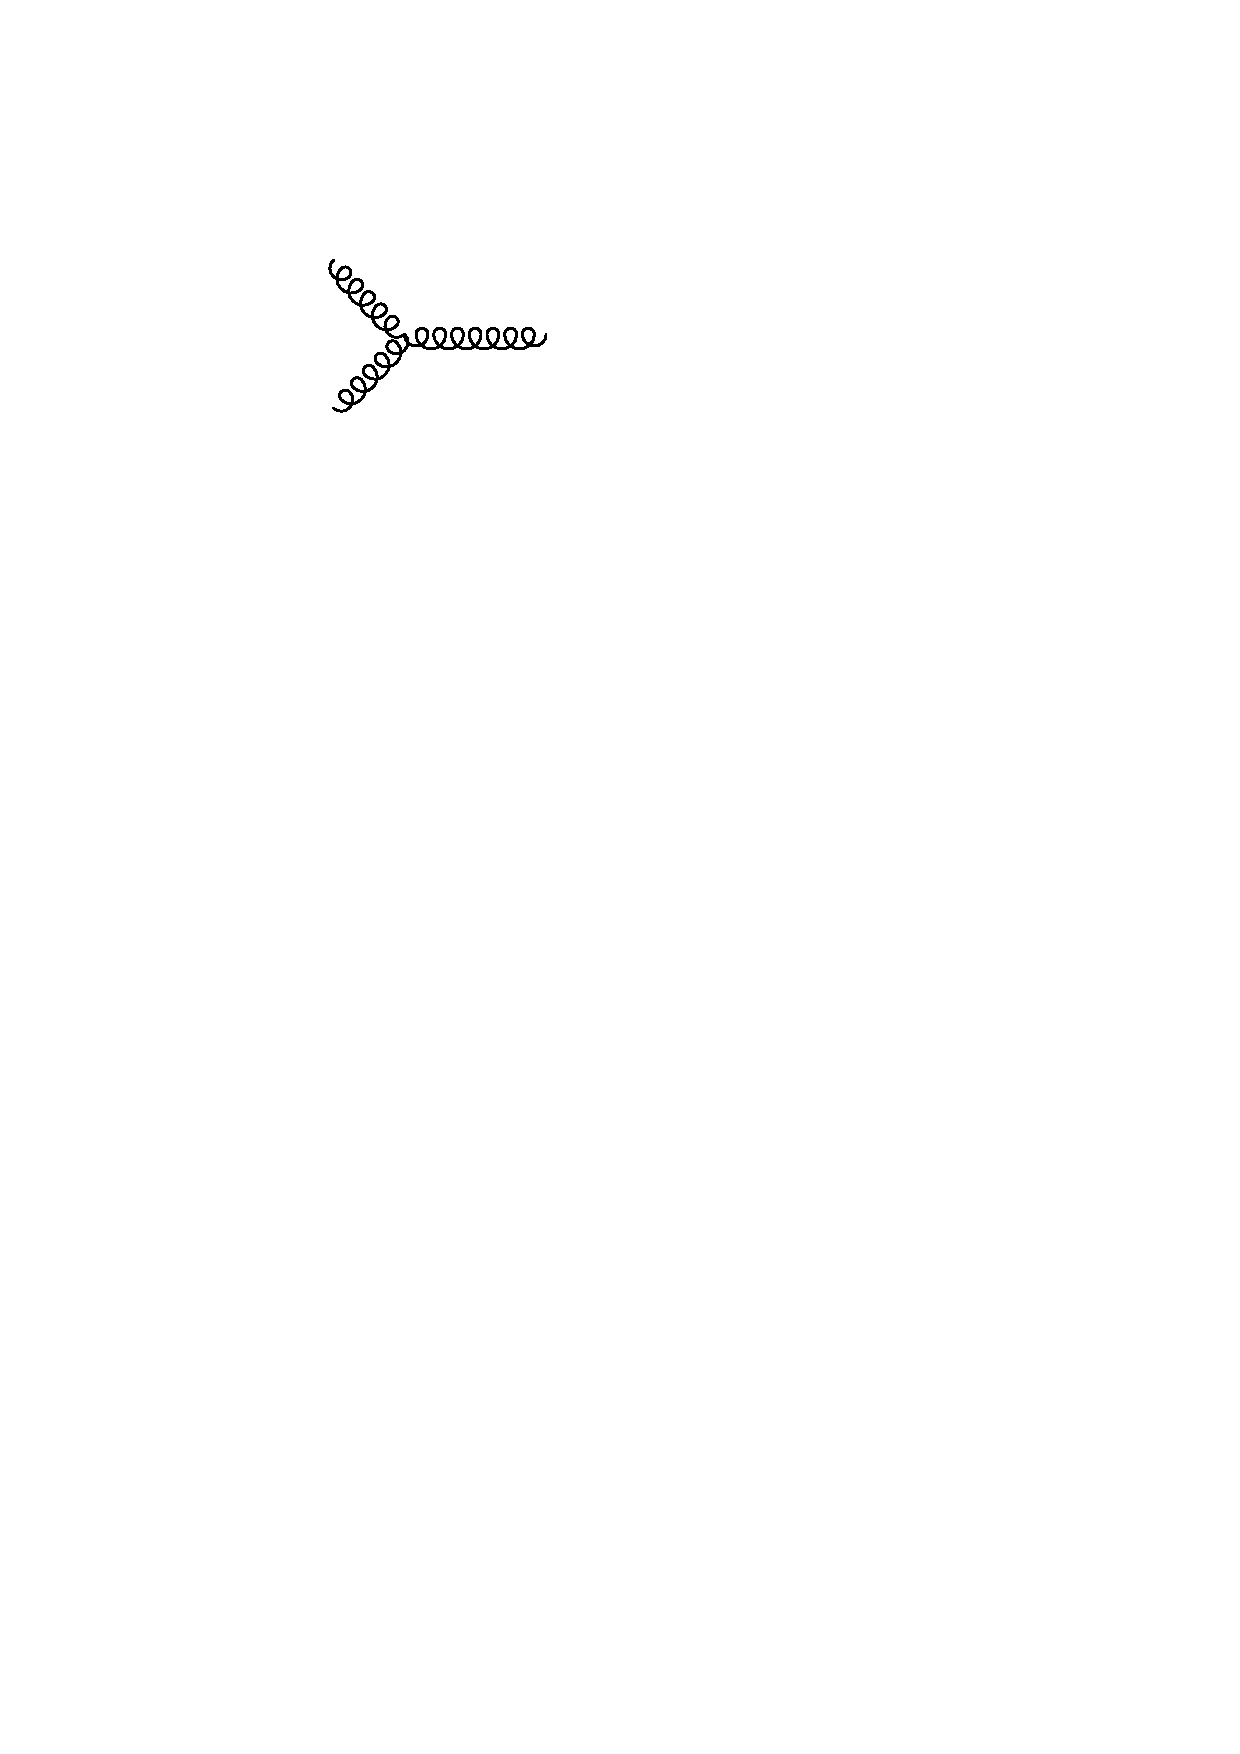
\includegraphics[width=0.3\textwidth]{fig/strongforce/gluon_three.pdf}

\includegraphics[width=0.3\textwidth]{fig/strongforce/gluon_four.pdf}
\end{center}
and the strength of the self-interaction is also characterised by $\alpha_s$. 
The self-interactions, together with the fact that $\alpha_s\sim 1$ means that the gluon field line density remains approximately constant with distance, in contrast to EM interactions where the field line density falls as $\frac{1}{r^2}$, as shown by the pictures below.
\begin{center}
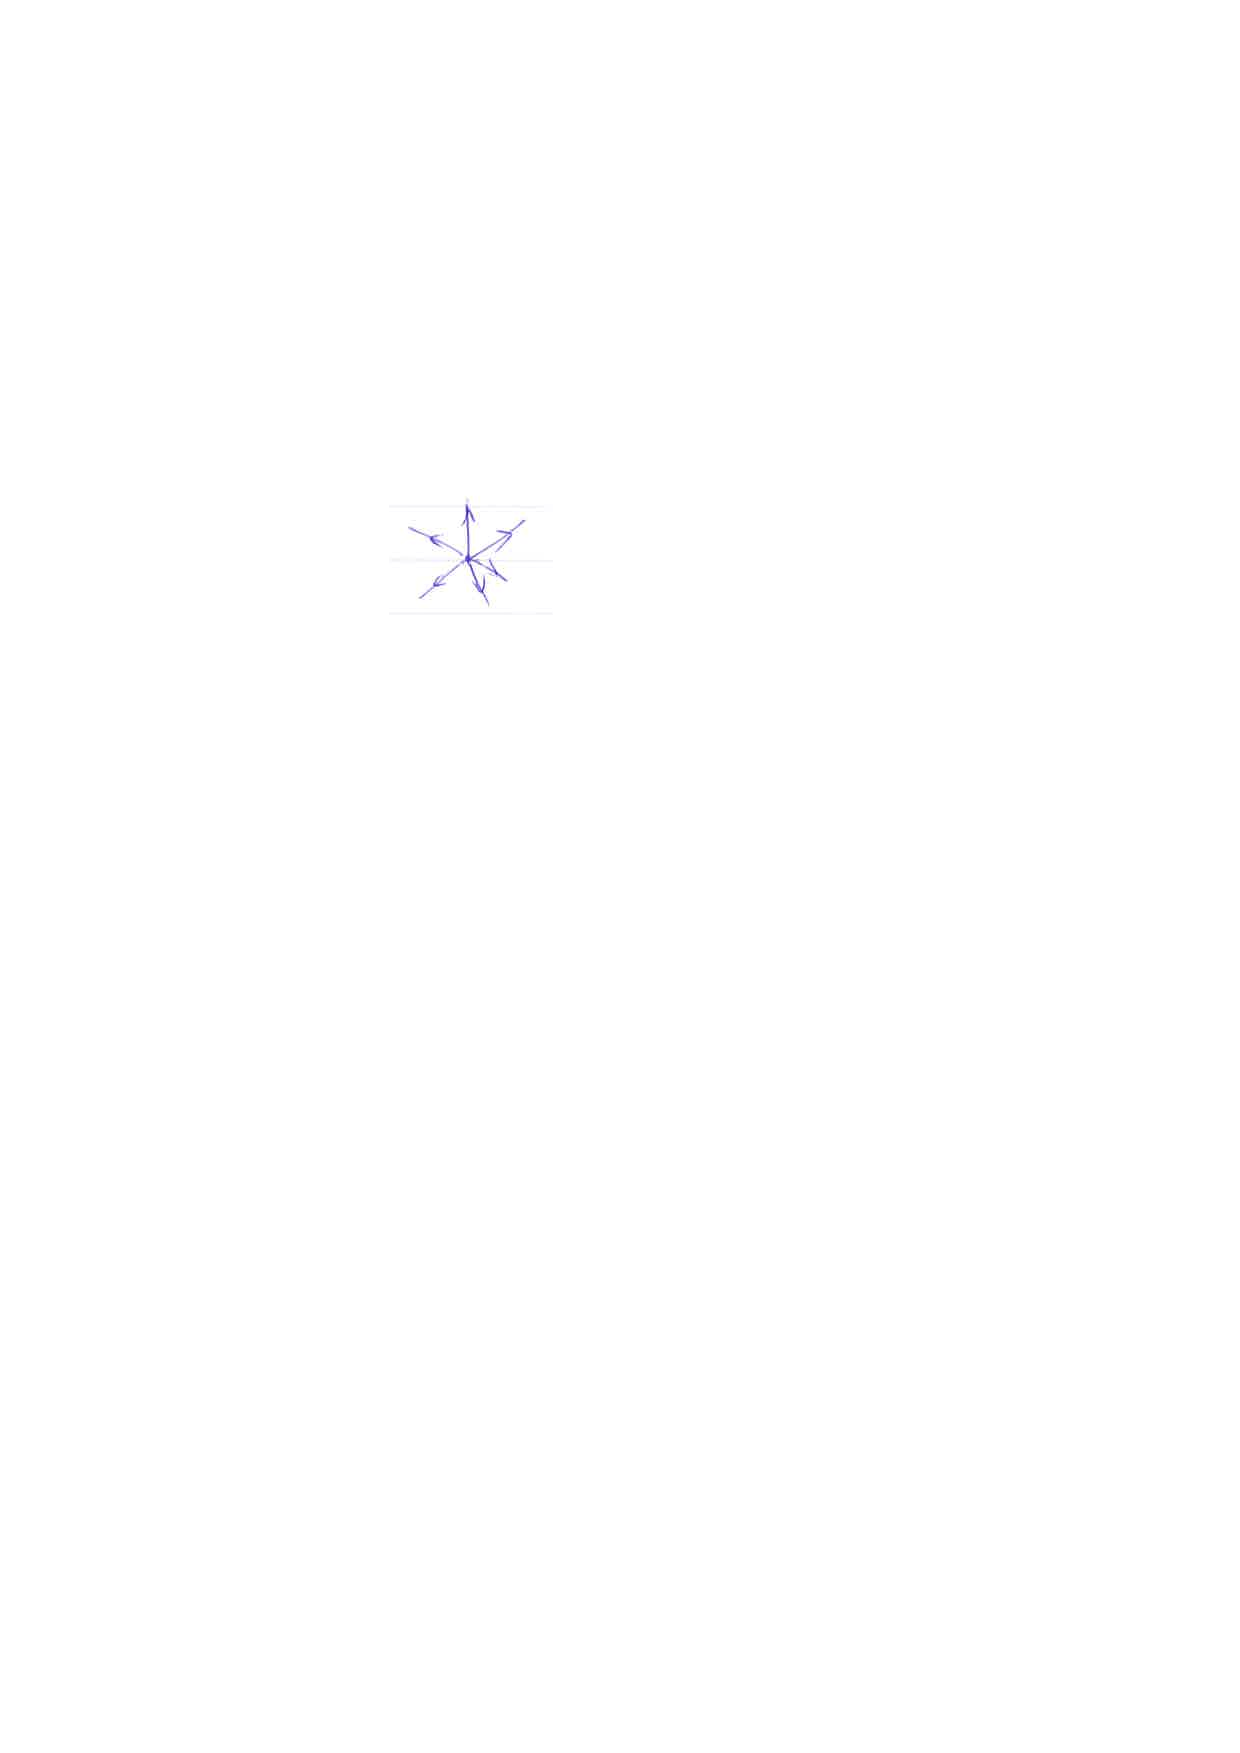
\includegraphics[width=0.3\textwidth]{fig/strongforce/em_line_density.pdf}
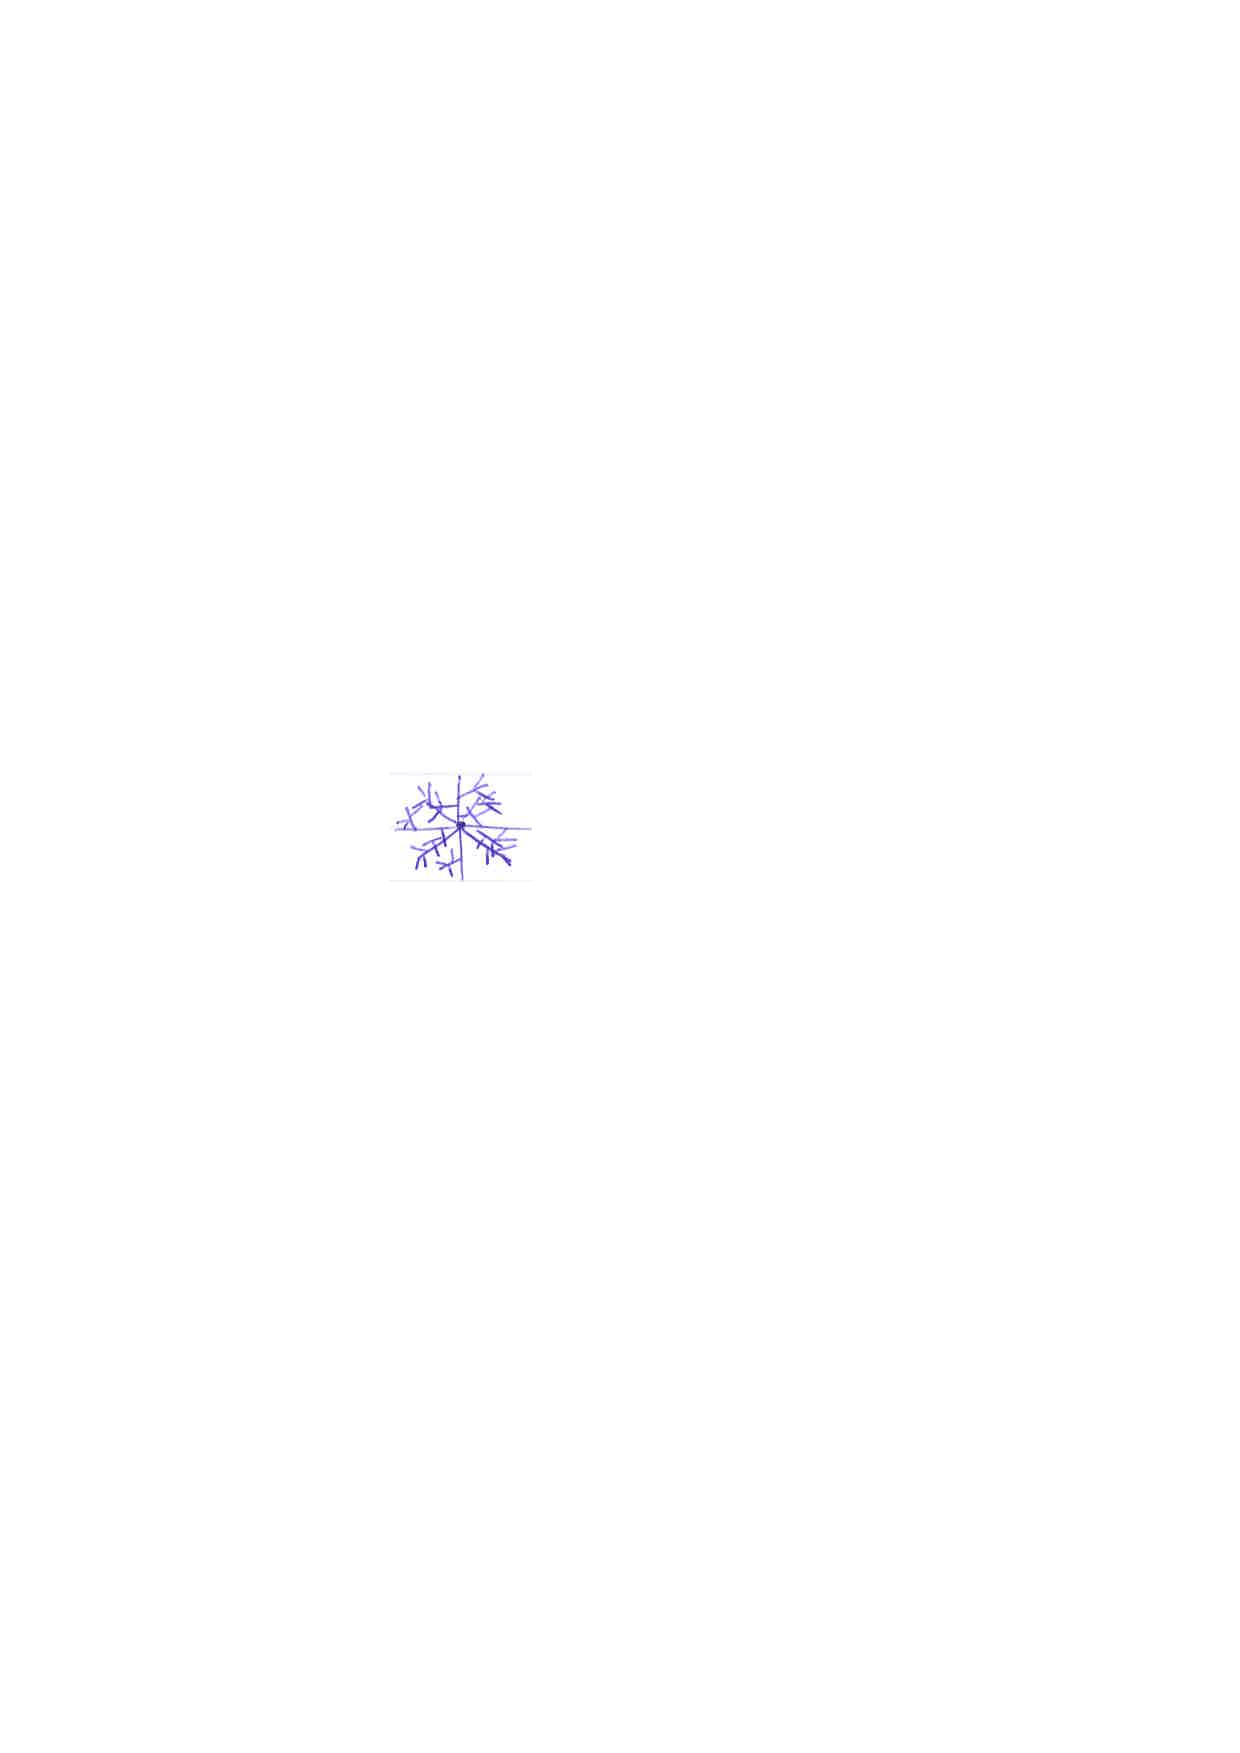
\includegraphics[width=0.3\textwidth]{fig/strongforce/strong_line_denstiy.pdf}\\
Pictures of EM field line density (left) and strong field line density (right)
\end{center}
So quarks can never be seen in complete isolation as they are constantly interacting with the field of the strong force. It takes around 1~GeV/fermi of energy to move a quark inside a hadron. As the masses of the up and down quarks are $\mathcal{O}(10)$~MeV, it is much more energetically favourable to produce quark-anti-quark pair which then forms a bound state rather than produce a free quark.

As it happens this is not the complete picture. As the energy (length)
scale of the strong process increases (decreases), the forces between
quarks becomes weaker. Therefore at large energies (small distances)
quarks can appear to move freely. This is why quarks within
hadrons appear to move freely within the hadron volume and the strong
coupling constant goes from $~1$ at an energy scale of 500~MeV to
$~0.1$ at 90~GeV. More information beyond the scope of the course can
be found in Appendix~\ref{sec:asymptotic_freedom}.

\subsection{Formation of jets}
\label{sec:FormationOfJets}
\begin{center}
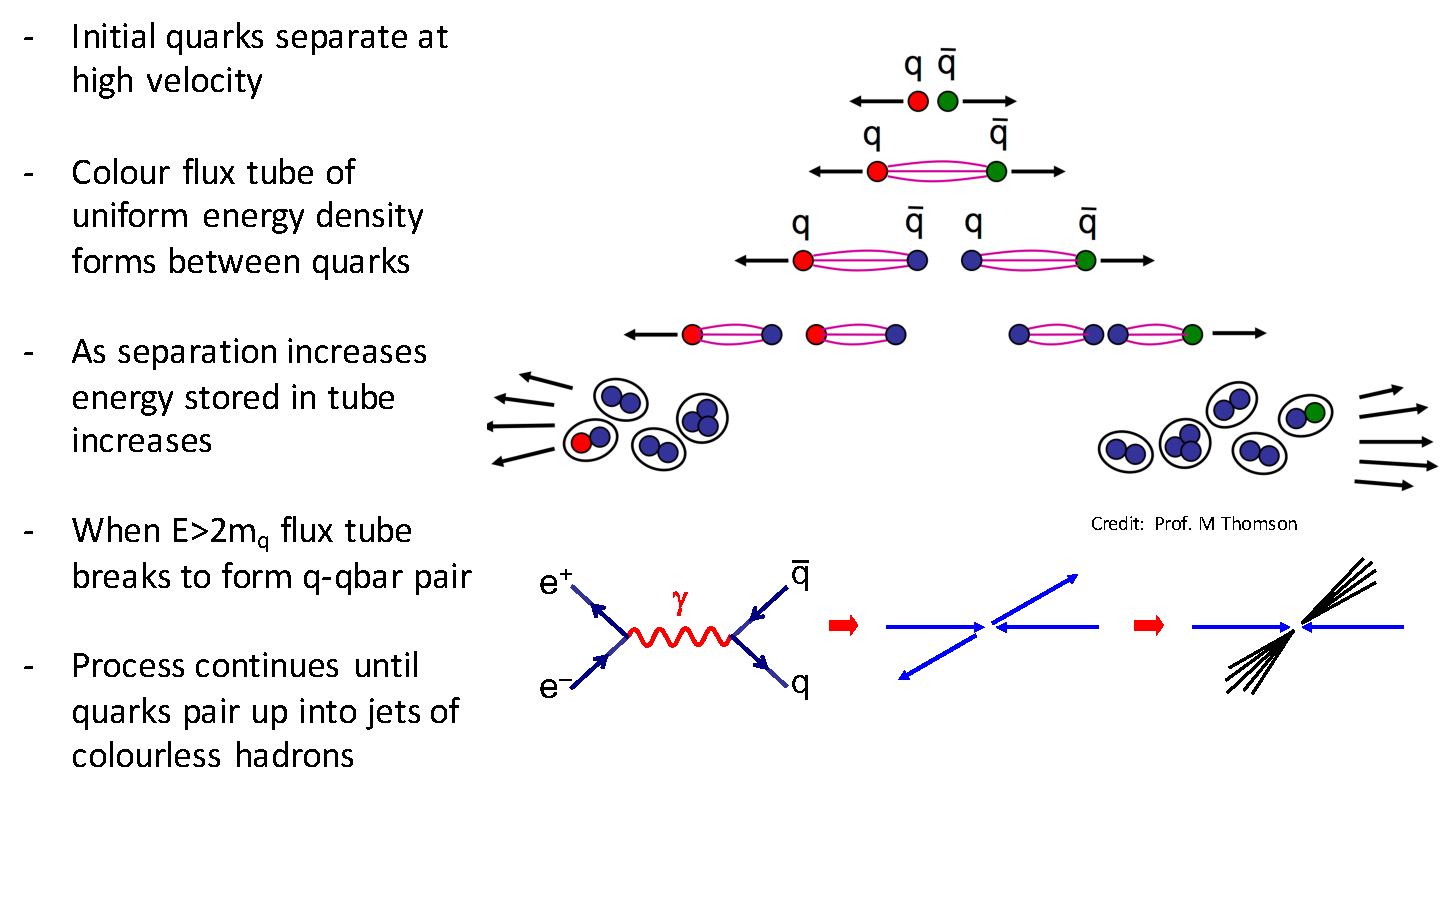
\includegraphics[width=0.97\textwidth]{fig/strongforce/jet_formation_2.pdf}
\end{center}

The picture below shows an example of a two-jet (di-jet) event produced from a collision of two protons at the LHC. 
\begin{center}
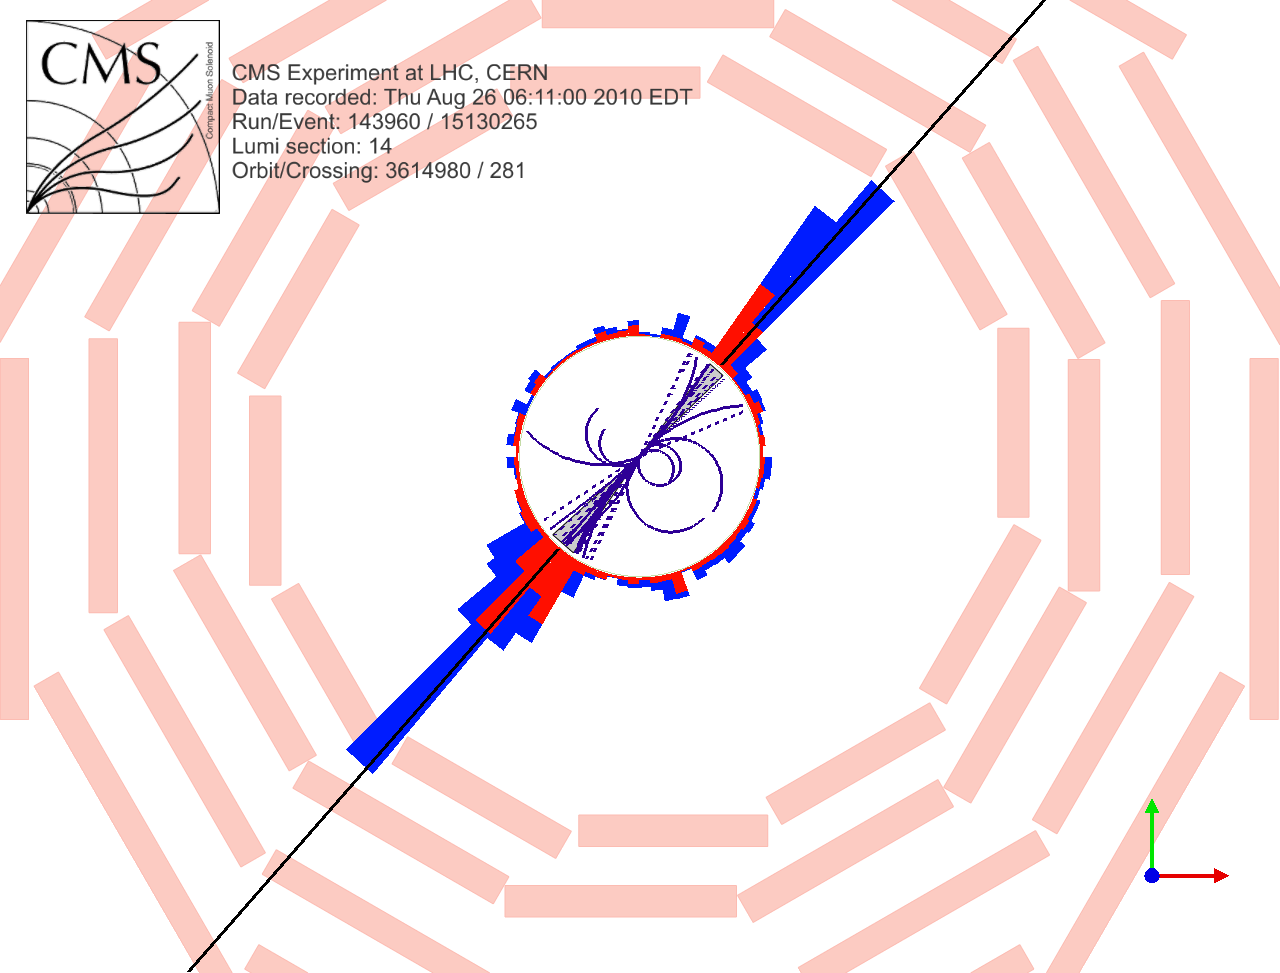
\includegraphics[width=0.4\textwidth]{fig/strongforce/cms_dijet.png}
\end{center}


\paragraph{Further evidence for colour:}
As you saw last year, further evidence for the existence of colour-charge stems from the measurement of the $R$-ratio defined as:
\[
R=\frac{\sum_q\sigma(e^+e^-\to q\bar{q})}{\sigma(e^+e^-\to\mu^+\mu^-)}=3\times\sum_q e_{q}^{2}
\]
where the factor of 3 accounts for the fact that the quark-anti-quark pair can be produced in 3 states ($r\bar{r}$, $b\bar{b}$, $g\bar{g}$) and the sum runs over quark types and depends on the centre of mass energy of the collision. For example at LEP1 where $\sqrt{s}=91$~GeV, the sum runs up to and including the $b$-quark, however as the $t$-quark has a mass of $\sim 175$~GeV, there is not enough energy to produce a pair of them. So 
\[
R=3\times\left[\left(\frac{1}{3}\right)^2+\left(\frac{2}{3}\right)^2+\left(\frac{1}{3}\right)^2+\left(\frac{2}{3}\right)^2+\left(\frac{1}{3}\right)^2\right]=\frac{11}{3}
\]
which agrees well with experimental measurements. If colour charge did not exist then the $R$ ratio should have been $\frac{11}{9}$.

\paragraph{Further evidence for the gluon:}
Further evidence for the existence of the gluon stems from the observation of events containing three jets. These could only have occurred if the final state of the interaction contained a quark, an anti-quark and a gluon, each individually resulting in a jet.
\begin{center}
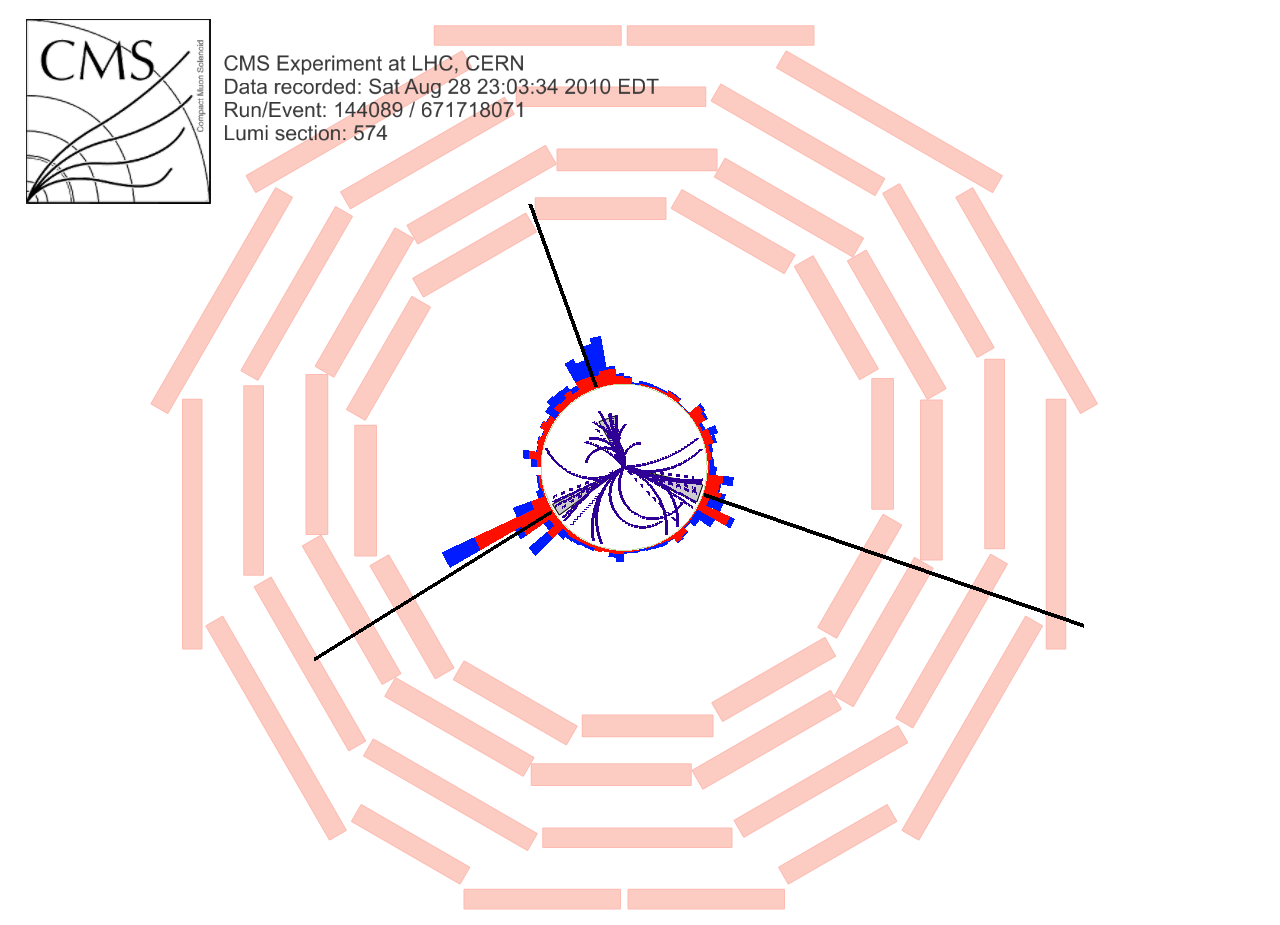
\includegraphics[width=0.5\textwidth]{fig/strongforce/cms_trijet.png}
\end{center}





\newpage

%% Week 5
\section{Particle Physics detectors}

In order to detect a particle it must interact with the material of the detector and transfer energy in some recognisable fashion.
\paragraph{Particle detection occurs via the energy loss of particles through the material they traverse.} In the end, all signals we record are electromagnetic signals. So we can discover charged particles. Neutral particles need to be converted to charged particles to be seen. This happens in an electromagnetic calorimeter with photons $\gamma \to e^+ e^-$, and in hadronic calorimeters via nuclear interactions that create charged pions and protons.

\paragraph{Possibilities}
\begin{itemize}
\item[(i)] EM charged particles $\rightarrow$ Ionisation, Bremsstrahlung$^*$, Cherenkov
\item[(ii)] Hadrons $\rightarrow$ Nuclear interactions$^*$ (equivalent to ones above the involving the strong force)
\item[(iii)] Photons $\rightarrow$ Pair production$^{**}$, Photoelectric effect, Compton effect
\end{itemize}
$^{(*)}$ Cause a shower of particles (see later).\newline
$^{(**)}$ Total energy loss via a single interaction converting into charged particles.\newline
Some examples of what these processes look like:

\begin{center}
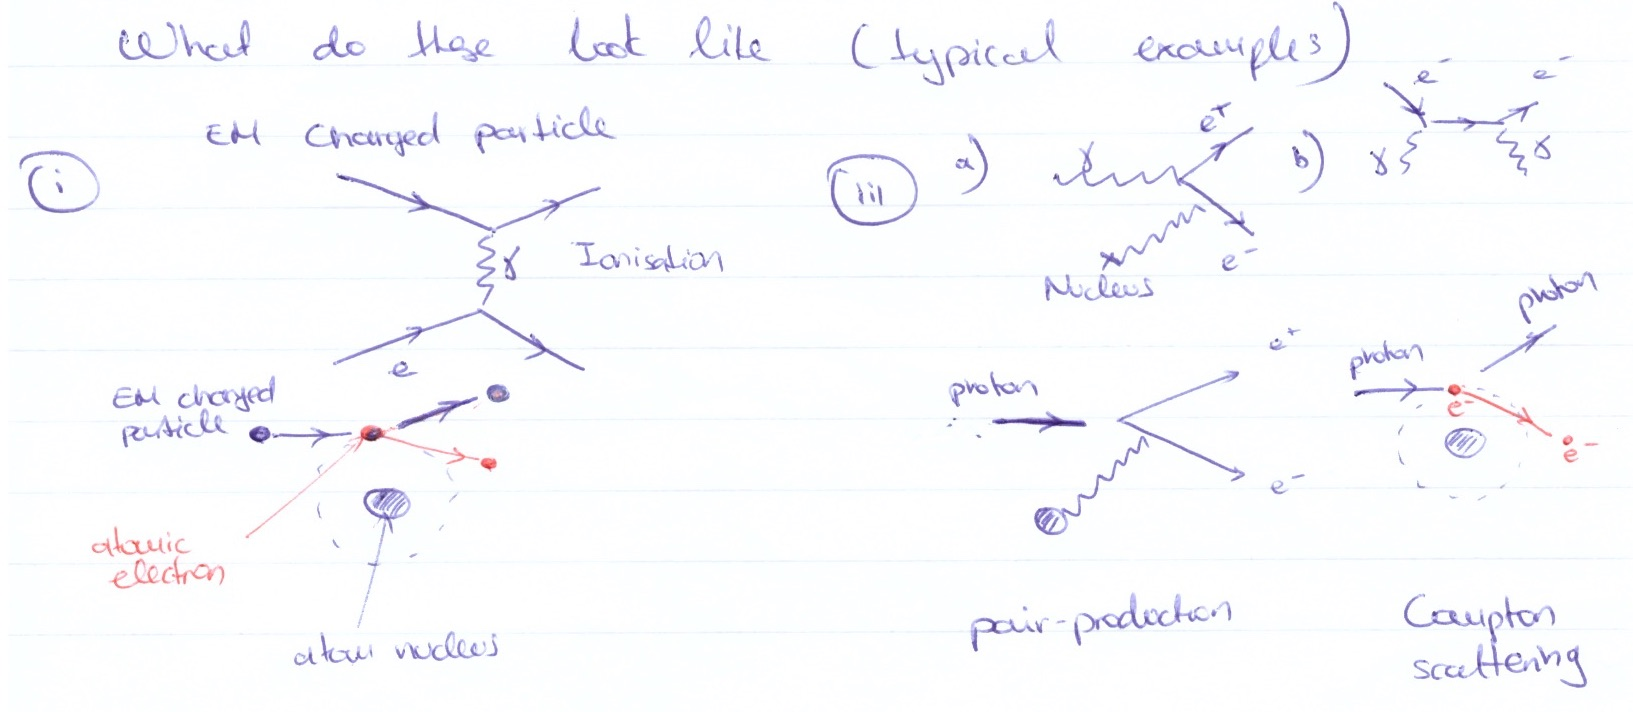
\includegraphics[width=0.95\textwidth]{fig/strongforce/matterinteractions/interactions1.jpg}\newline
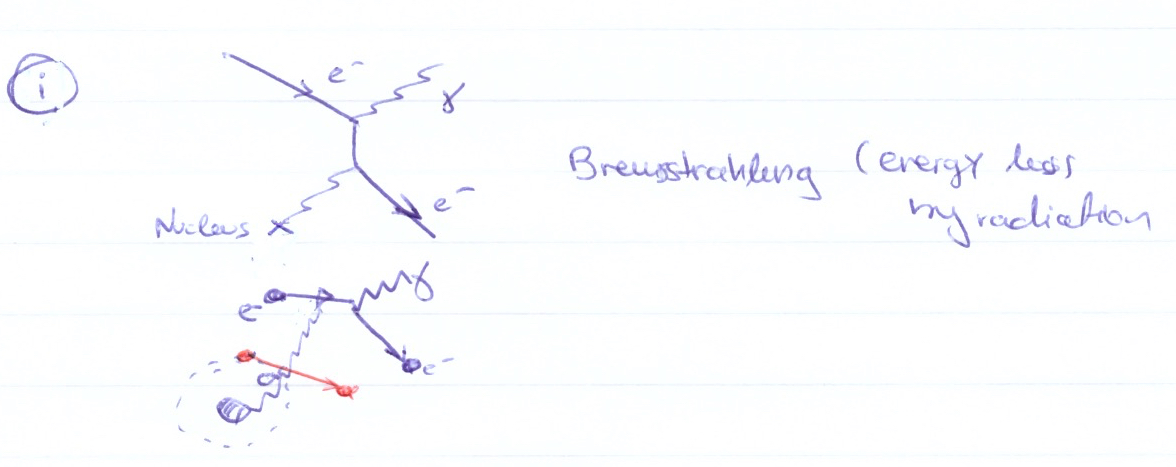
\includegraphics[width=0.8\textwidth]{fig/strongforce/matterinteractions/interactions2.jpg}
\end{center}

A lot more information of this section can be found in Appendix~\ref{sec:interaction_particle_matter} that is not examinable but quite interesting!


\subsection{Putting together a particle physics detector}
\label{sec:detectorSummary}
\begin{center}
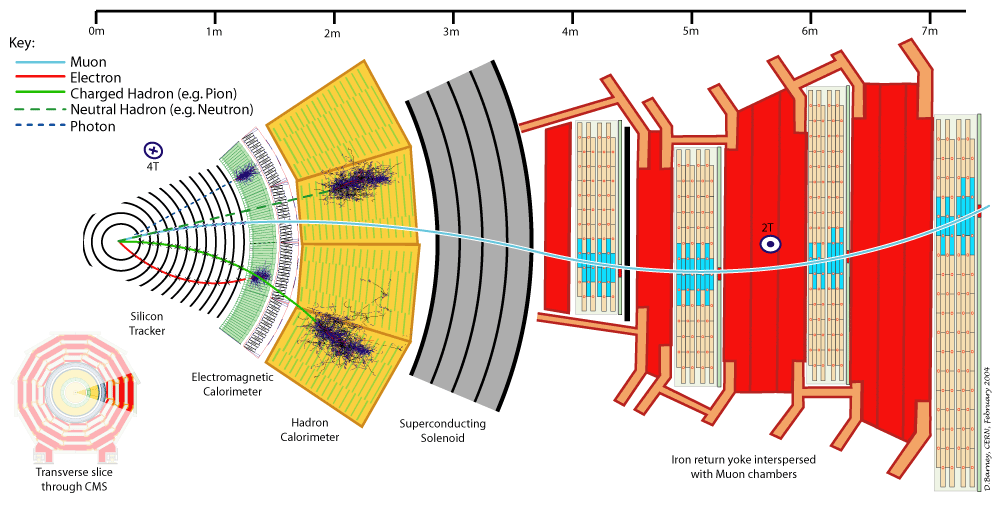
\includegraphics[width=0.95\textwidth]{fig/detector/cms_slice.png}
\end{center}

The inner most part of a detector is typically made up of relatively low radiation and interaction length material aimed at making a precise measurement of the initial collision point and of subsequent decay vertices. This is achieved by reconstructing the trajectories of outcoming charged particles as they deposit energy via ionisation. They are called ``vertex detectors'' and are typically made up of silicon pixel or strip sensors. 

Following the vertex detectors, one finds further detectors aimed at reconstructing the trajectories of charged particles by detecting ionisation energy as the particles traverse through them (``Tracking detectors''). By placing a magnetic field and measuring how the trajectory of the particles bends, we can get an estimate of their momentum.

Past the tracking detectors one can place RICH detectors (e.g at LHCb) aimed at measuring the speed of the particle, and combining with the measurement of the momentum obtain an estimate of the particle's mass and hence its type. One can also place an ECAL after the tracking (and after the RICH systems) to measure the energies of photons and electrons. As hadrons have masses much larger than the electron mass, they will not have an EM shower in the ECAL and will not form a hadronic shower either, as the typical interaction length ($\lambda$) of the ECAL is much too small (ECALs are less dense than HCALs). 

After the ECAL follows the HCAL. In the HCAL hadrons like pions, Kaons and protons will perform a hadronic shower, allowing for the measurement of their energies. Energies of jets of hadrons initiated by quarks and gluons, are measured by combining information from the tracking systems and calorimeters.

Muons are a special case. As $m_\mu\sim m_\pi\gg m_e$ and muons do not undergo strong interactions, they pass through the ECAL and HCAL by simply depositing a minimum amount of ionisation energy. Therefore in order to detect muons, detection systems aimed at measuring deposits of ionisation energy are placed after the HCAL, allowing for both the identification of muons (as mainly muons would reach the outer parts of the detectors) as well as the measurement of the momentum as the muon bends in the magnetic field. Muons are therefore very easy to distinguish from other particles: They are the one charged particle that makes it through all the mass in the calorimeters and survives until the muon detectors. Particle physicists love decays with muons int he final state!

\begin{center}
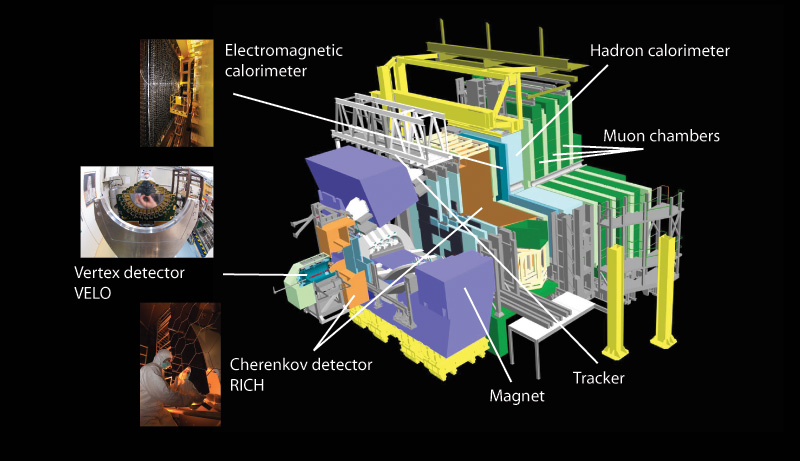
\includegraphics[width=0.95\textwidth]{fig/detector/lhcb_detector.png}
\end{center}
The figure below shows a similar configuration for the LHCb detector.

\subsection{Missing transverse momentum (or energy)}
This has already been discussed in \secref{sec:missingEt}, but is repeated here under a slightly different angle, because it also belongs into the detector section, and because it is important.

In hermetic ($4\pi$) detectors like CMS and ATLAS, particles that only very rarely interact
with matter (such as neutrinos and particles proposed in theories beyond the Standard Model such as Supersymmetry or hypothesised Dark Matter candidate particles) are detected by their absence. What do we mean by that? 

In a $pp$ collision (or any collision) where the protons are primarily only have momentum along the horizontal axis, the total initial momentum transverse to the direction of the protons is zero. Therefore after the collision, momentum should be conserved and thus the total momentum obtained by summing over all the outcoming particles from the collision (this is why detectors like CMS that completely surround the collision are important), transverse to the direction of the protons ie 
\[{\rm Missing\,\,Transverse\,\,Momentum}=-\sum_{\rm i=1..N_{\rm particles}} p_{T}^{i}\]
should add up to zero. If it does not then it means that particles where produced which did not interact with the detector. Such particles could have been known neutrinos or, depending on the amount of missing energy, momentum could be Dark Matter candidates.
The figure below, is a $t\bar{t}$ event from CMS where each of the $t$-quarks decay to a $b$ quark (which forms a jet) and a $W$ boson which subsequently decays to a $\mu$ and a $\nu_{\mu}$. The sum of the momenta that the two $\nu$'s carry (one from the $t$ and another from the $\bar{t}$) is inferred by the mis-balance of momentum (or equivalently energy) in the transverse plane and is denoted by the purple arrow labelled $\cancel{\rm E_{T}}$.
\begin{center}
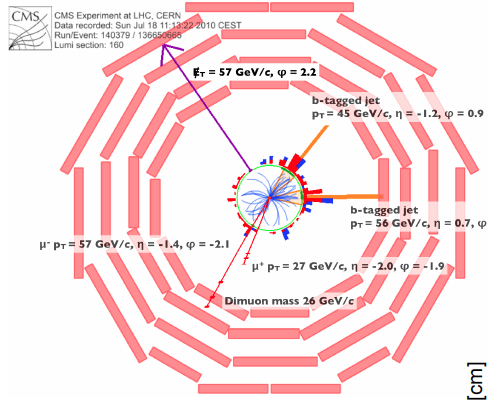
\includegraphics[width=0.75\textwidth]{fig/detector/met_cms.png}
\end{center}

An example of a process that makes use of all detector components of the detector is the production of top quarks at the LHC. Top quarks have a very short lifetime. 
\[\tau_{t}=5\times 10^{-25}s\]
However the time at which QCD confinement acts (ie the time scale in which a quark binds into a hadron) can be calculated as follows:

QCD confinement takes place at an energy scale 
\[
\Lambda_{QCD}=200~{\rm MeV}.
\]
We can convert this energy scale into a timescale using 
\[
\hbar c=200~{\rm MeV~fm}
\]
(this is something you should commit to memory as it is a very useful quantity for a particle physicist).
Therefore
\[
\tau_{QCD}=\hbar c\times\frac{1}{c\Lambda_{QCD}}=3\times 10^{-24}s
\]
As $\tau_{QCD}<\tau_{t}$, the top quark decays before it has a change to form a bound state! 

Due to the CKM elements involved, the top quark predominantly decays to a b-quark 
\[t\rightarrow b W\]
where the $b$-quark will in turn produce a jet of particles which contains at least one hadron with a $b$-quark. This so called $b$-jet can be identified both through the stream of hadrons producing tracks in the tracking system and energy depositions in the calorimeters, as well as through the displaced vertex formed by the decay products of the $B$-hadron.
The $W$ will in turn decay into a lepton or a pair of quarks. In the case that the $W$ decays to a lepton and a neutrino, the neutrino escapes the detector and its existence is inferred through missing transverse energy.

%

%%%In order to detect a particle it must interact with the material of the detector and transfer energy in some recognisable fashion.
%%%\paragraph{Particle detection occurs via the energy loss of particles through the material they traverse.}
%%%
%%%\paragraph{Possibilities}
%%%\begin{itemize}
%%%\item[(i)] EM charged particles $\rightarrow$ Ionisation, Bremsstrahlung$^*$, Cherenkov
%%%\item[(ii)] Hadrons $\rightarrow$ Nuclear interactions$^*$ (equivalent to ones above the involving the strong force)
%%%\item[(iii)] Photons $\rightarrow$ Pair production$^{**}$, Photoelectric effect, Compton effect
%%%\end{itemize}
%%%$^{(*)}$ Cause a shower of particles (see later).\newline
%%%$^{(**)}$ Total energy loss via a single interaction converting into charged particles.\newline
%%%Some examples of what these processes look like:
%%%
%%%\begin{center}
%%%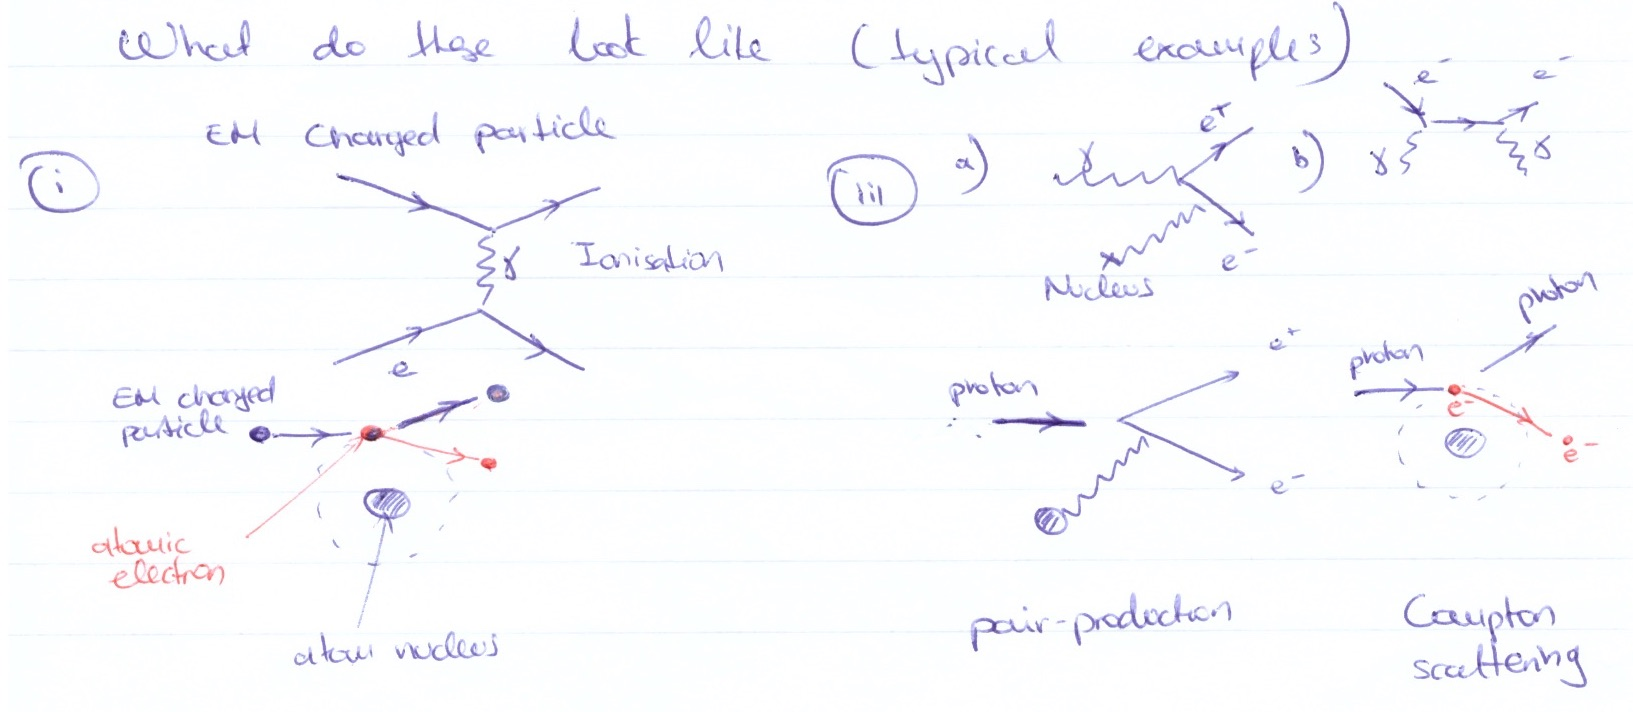
\includegraphics[width=0.95\textwidth]{fig/strongforce/matterinteractions/interactions1.jpg}\newline
%%%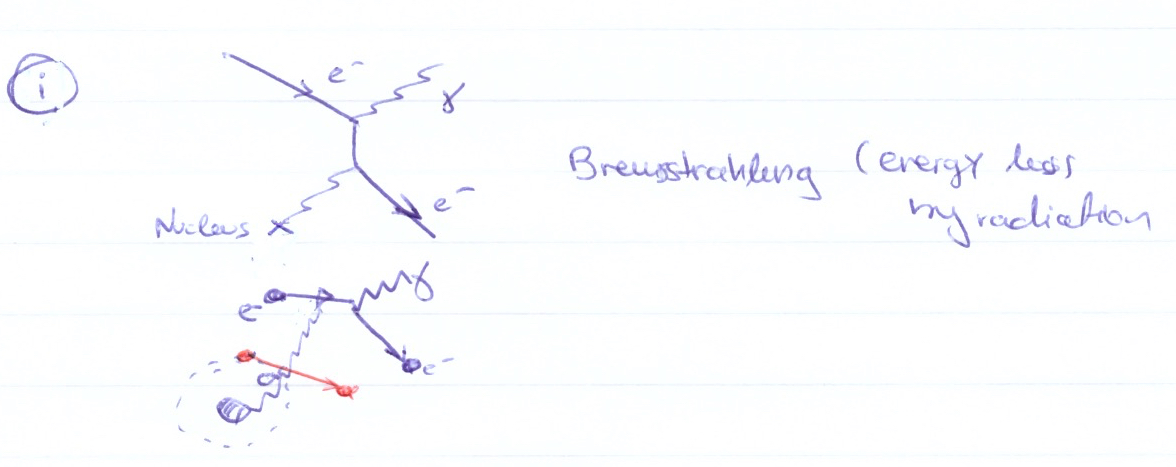
\includegraphics[width=0.8\textwidth]{fig/strongforce/matterinteractions/interactions2.jpg}
%%%\end{center}
%%%
%%%
%%%\subsubsection{Energy loss by ionisation}
%%%We can quantify the energy loss of a particle traversing through the detector, by looking at the average rate of energy lost per unit distance.
%%%
%%%
%%%For an incident particle of charge $ze$ with mass $M>>m_e$, losing energy by ionising atomic electrons in a material with atomic number $Z$ we can use the Bethe-Bloch equation:
%%%
%%%\begin{equation}
%%%\label{eq:bethebloch}
%%%<\frac{dE}{dx}>\approx -2C\frac{m_ec^2Zz^2}{\beta^2A}\rho\left[\frac{1}{2}\log\frac{2m_ec^2\beta^2\gamma^2T_{\rm max}}{I^2}-\beta^2-\frac{\delta(\beta\gamma)}{2}\right]
%%%\end{equation}
%%%with \[C=2\pi N_A\frac{e^2}{4\pi\epsilon_0m_ec^2}.\] 
%%%$I$ is the mean ionisation potential ie $h<\nu_e>$ (given by $\sim10Z$~eV for $Z>20$), $\rho$ is the density of the material, $\delta(\beta\gamma)$ is a density correction term because the incoming particle can polarise the medium, and $T_{\rm max}$ is the maximum energy transfer in a single collision given by
%%%\[
%%%T_{\rm max}=\frac{2m_ec^2\beta^2\gamma^2}{[1+2\gamma m_e/M +(m_e/M)^2].}
%%%\]
%%%For $\frac{\gamma m_e}{M}<<1$, $T_{\rm max}$ can be simplified to
%%%\[
%%%T_{\rm max}\sim2\gamma^2\beta^2m_ec^2.
%%%\]
%%%
%%%\exercise{
%%%One can approximate the picture of a charged particle of mass $M \gg m_e$ with charge $ze$ traversing a material of atomic number $Z$, as an infinitely long cylinder of radius $b$, with charge uniformly distributed  on the surface, surrounding the charged particle which sits in the middle. Let us consider this charged particle interacting with an electron in the medium.
%%%\begin{center}
%%%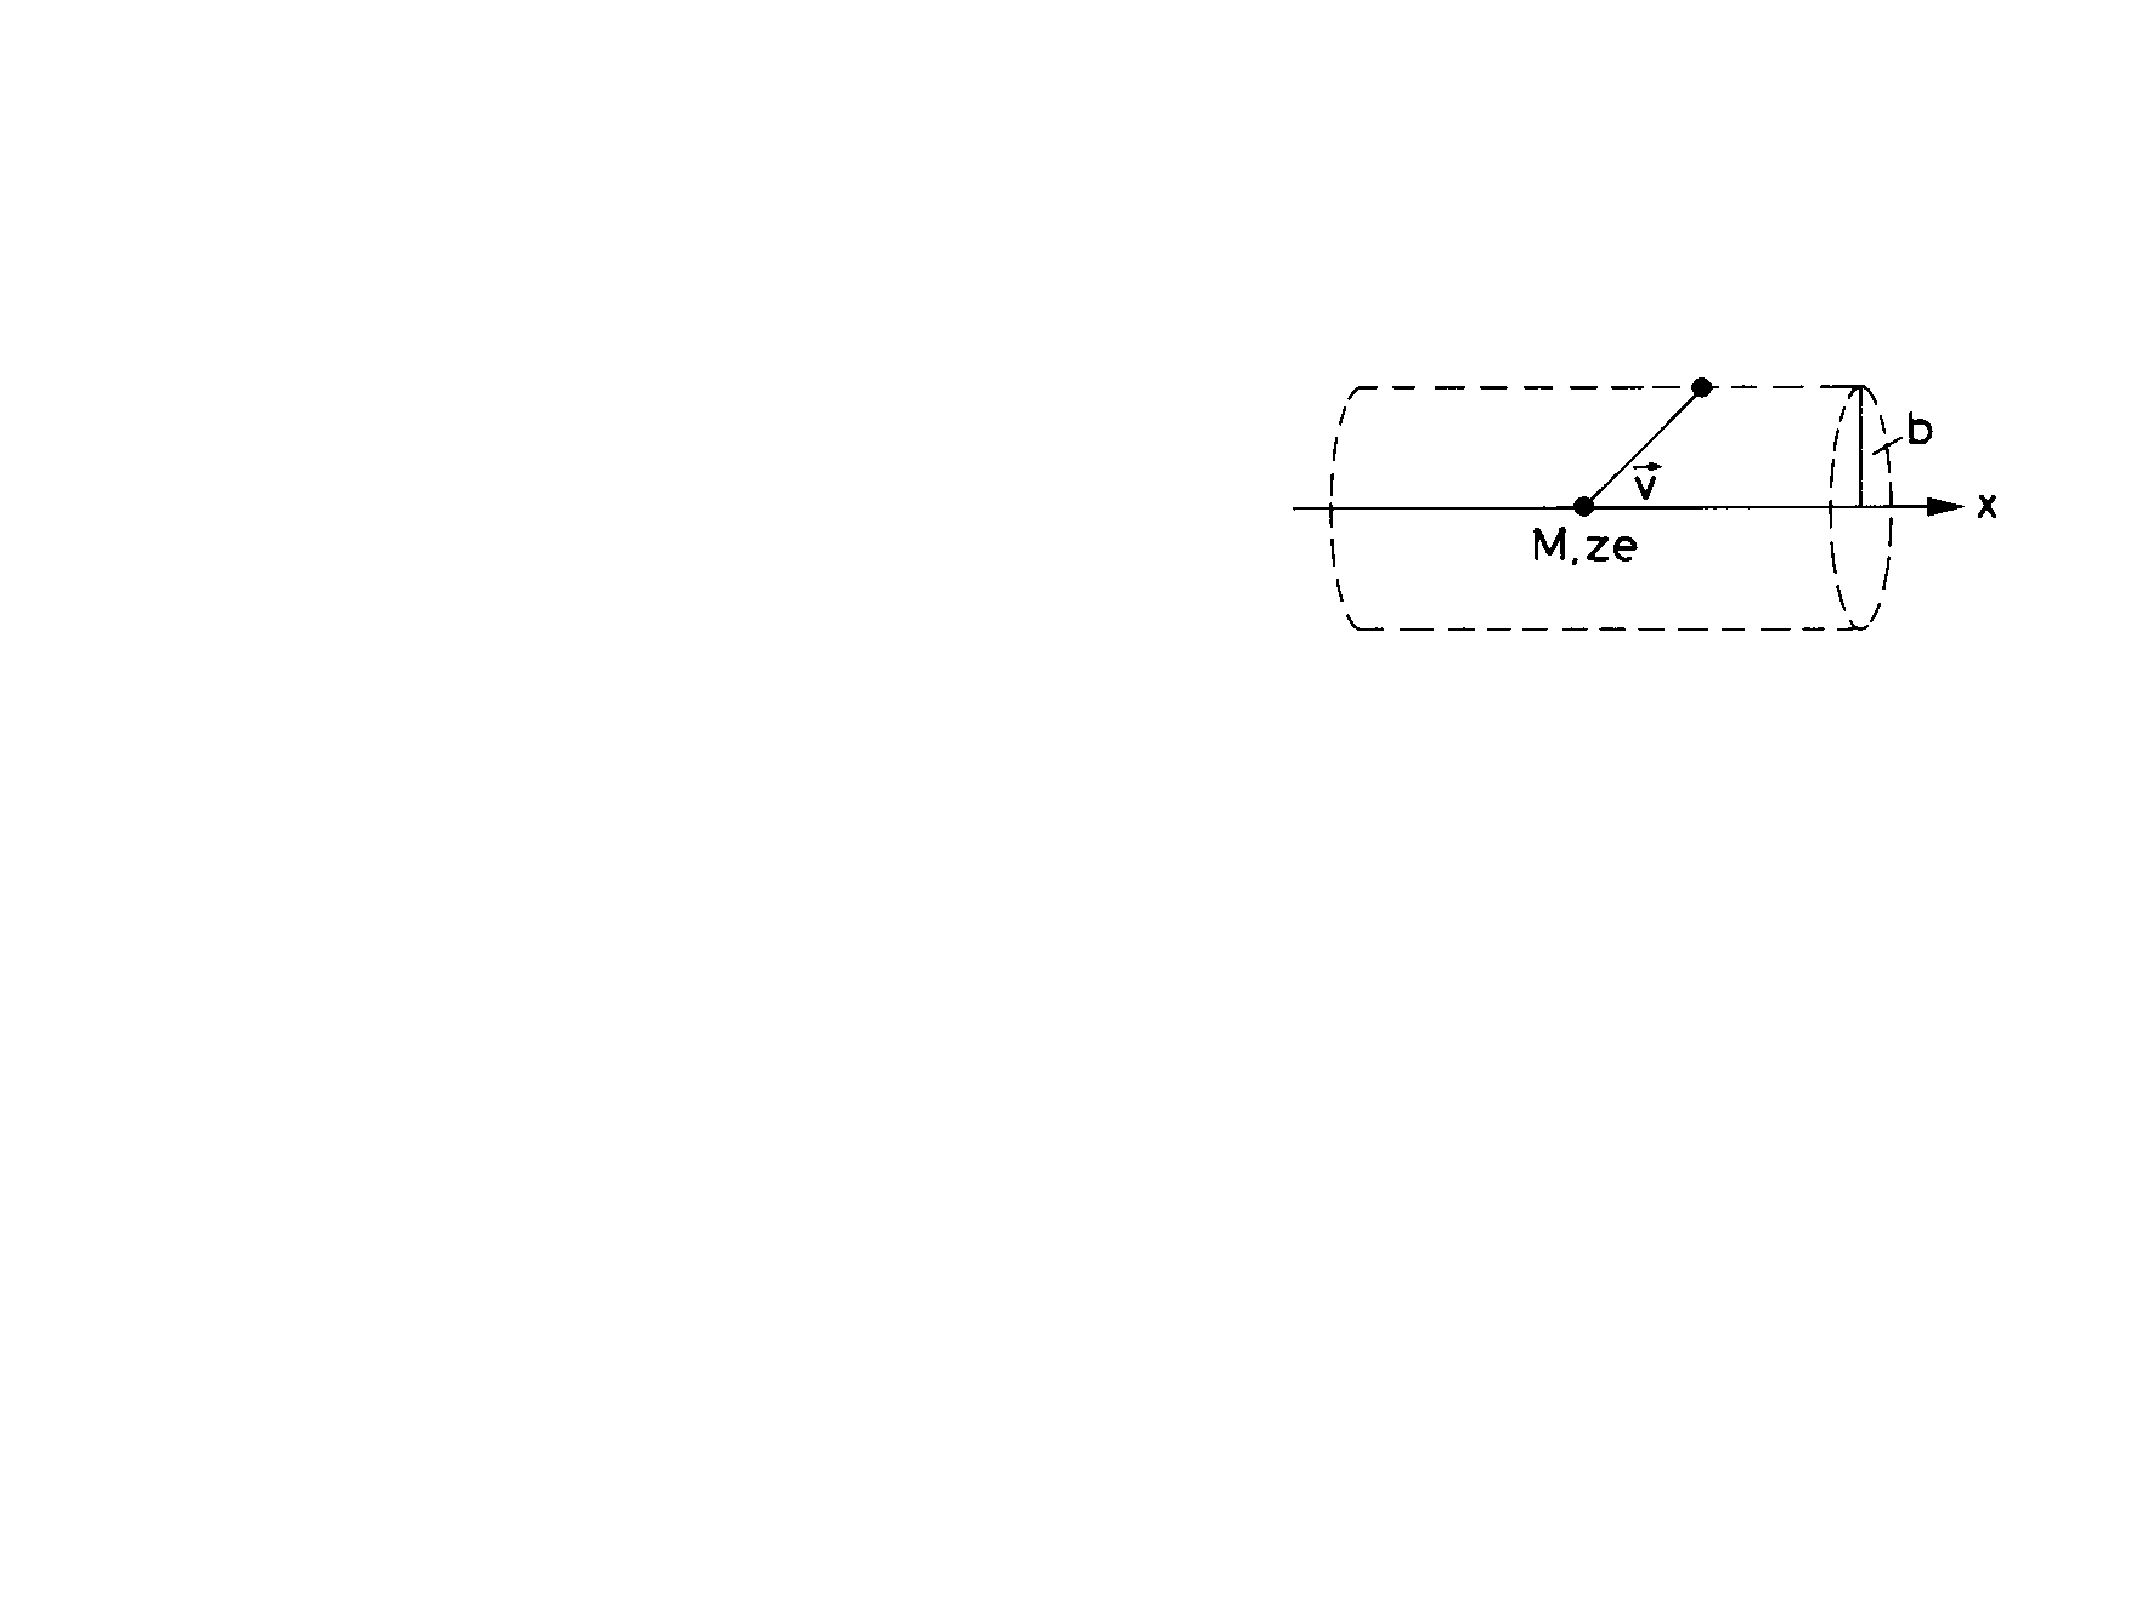
\includegraphics[width=0.5\textwidth]{fig/strongforce/matterinteractions/particle_in_cylinder.pdf}
%%%\end{center}
%%%By applying Gauss's law, show that the momentum transfer perpendicular to the motion of the charged particle, defined by $\Delta p_{\perp}=\int F_{\perp} dt$, is given by $\frac{2ze^2}{bv}$, where $v$ is the speed of the charged particle. Show that $\Delta p_{\parallel}=0$. You can use the fact that in natural units $\epsilon_0=\frac{1}{4\pi}$.\\\\
%%%
%%%Consider now a section of this cylinder of length $dx$. Also let's assume the surface of the cylinder has a width $db$. Show that if the electron density of the cylinder in $n$, the number of electrons contained within this cylinder section is $N_e=n(2\pi b)dbdx$. Therefore show that the energy loss per path length $dx$ traversed by the charged particle is given by:
%%%\[dE=-\frac{4\pi n z^2 e^4}{m_e v^2}\frac{db}{b}dx\]
%%%Hint: Energy transferred onto a single electron on surface of cylinder is given by $\Delta E=\frac{\Delta p^2}{2m_e}$\\\\
%%%
%%%By integrating between $b_{\rm min}$ and $b_{\rm max}$ we have:
%%%\[
%%%\frac{dE}{dx}=-\frac{4\pi n z^2e^4}{m_ev^2}\log\frac{b_{\rm max}}{b_{\rm min}}
%%%\]
%%%The question now is what are sensible values for $b_{\rm min}$ and $b_{\rm max}$. 
%%%If $b$ becomes so large that the energy transfer is lower than the mean energy required to ionise an electron (given by $I=h<\nu_e>$). The minimum value of $b$ occurs when the maximum possible energy transfer occurs. From relativistic energy-momentum conservation, the maximum energy transferred is $\approx 2\gamma^2\beta^2m_e$ (in natural units)
%%%Therefore show that:
%%%$\displaystyle \frac{dE}{dx}=-\frac{4\pi z^2 e^4}{m_e \beta^2}n\frac{1}{2}\log\frac{2m_e\beta^2\gamma^2}{h<\nu_e>}$
%%%}
%%%
%%%\paragraph{Example: Pions in Cu.} Features are common for all materials
%%%
%%%\begin{center}
%%%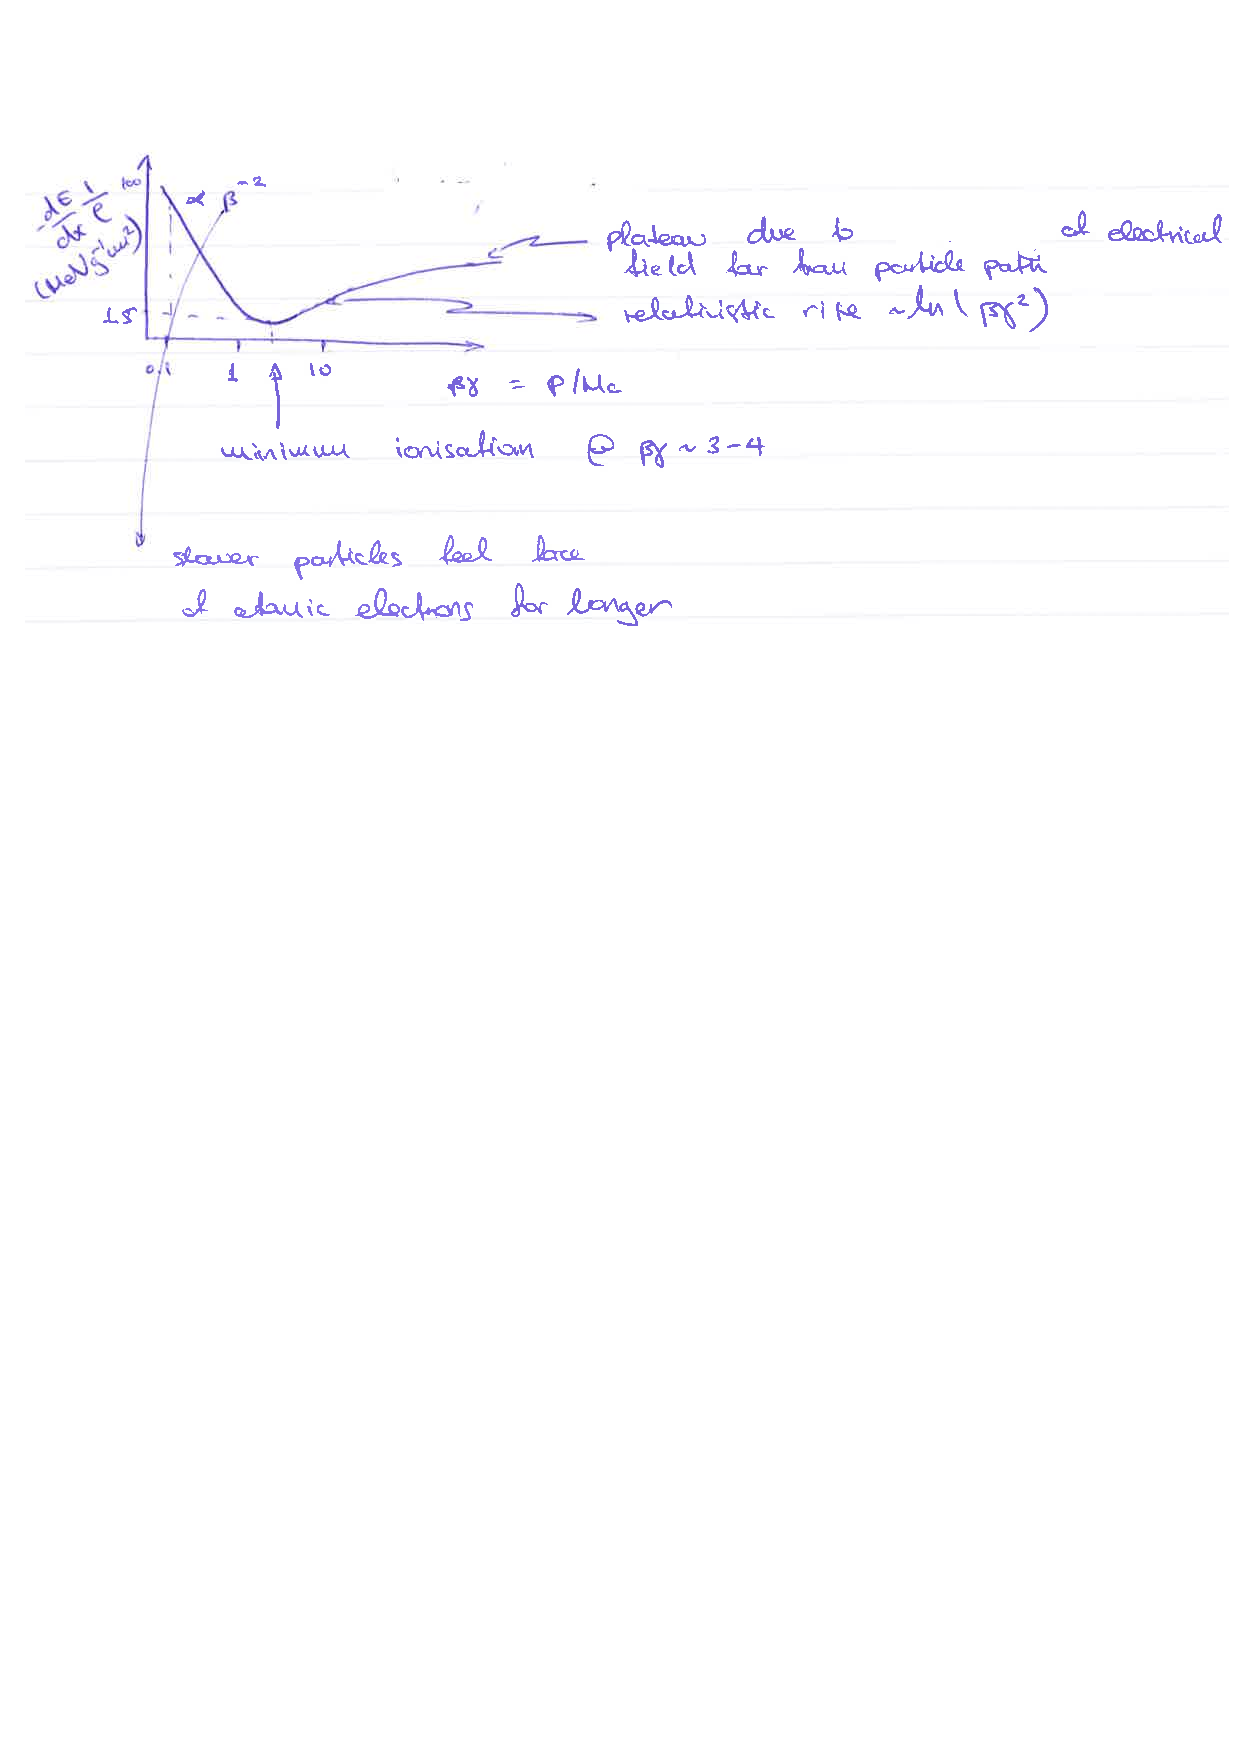
\includegraphics[width=0.95\textwidth]{fig/strongforce/matterinteractions/interactions4.pdf}
%%%\end{center}
%%%
%%%Let us consider some key features, ignoring the $-\beta^2$ and $-\delta(\beta\gamma)$ terms for a moment we have:
%%%\[<\frac{dE}{dx}>\propto -\frac{1}{\beta^2}\log{({\rm const}\cdot\beta^2\gamma^2)}.\]
%%%\begin{itemize}
%%%\item The $1/\beta^2$ fall is due to the fact that slower particles feel the force of atomic electrons for longer. 
%%%\item The $\log{({\rm const}}\cdot\beta^2\gamma^2)$ term is a relativistic rise which comes about due to the fact that high energy particles the electric field transverse to the direction of motion of the particle increases, thus increasing the probability of an interaction.
%%%\end{itemize}
%%%The plateau of the $<\frac{dE}{dx}>$ distribution for $\beta\gamma>10$ is due to the fact that the incoming particle polarises the medium thus shielding the electric field far from the particle path, thus cutting the long range contribution. This is the reason behind the $\delta(\beta\gamma)$ term.  
%%%
%%%The figure below shows the energy lost via ionisation in a sub-detector of ALICE (A Large Ion Collider Experiment) at CERN. It is evident that if one knows the momentum of the incoming particle, then the energy lost through ionisation can distinguish between different incoming particles.
%%%\begin{center}
%%%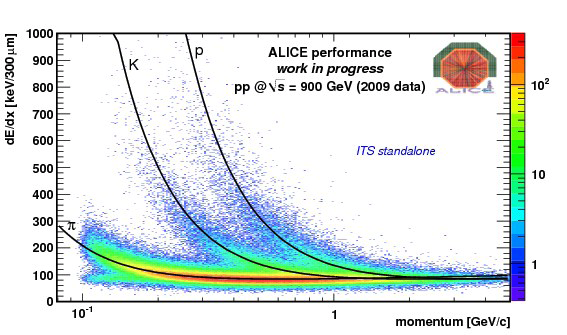
\includegraphics[width=0.95\textwidth]{fig/strongforce/matterinteractions/alice_dedx.png}
%%%\end{center}
%%%
%%%\paragraph{Multiple scattering through small angles: time permitting}
%%%A charged particle traversing a medium feels the Coulomb force of nuclei and hence gets deflected. As it gets multiple deflections from multiple nuclei as it traverses the material, this effect is called ``multiple scattering''. The deflection angle follows a Gaussian distribution centred at zero with a width $\theta_0$ given by:
%%%\[
%%%\theta_0\propto \frac{z\sqrt{x}}{vp}(1+0.038\log{x}+{\rm const})
%%%\]
%%%where $z$ is the charge of the particle in multiples of electric charge, $x$ is the distance travelled, $p$ is the momentum and $v$ is the speed of the particle traversing the medium. A pictorial view of the deflection can be seen below.
%%%
%%%\begin{center}
%%%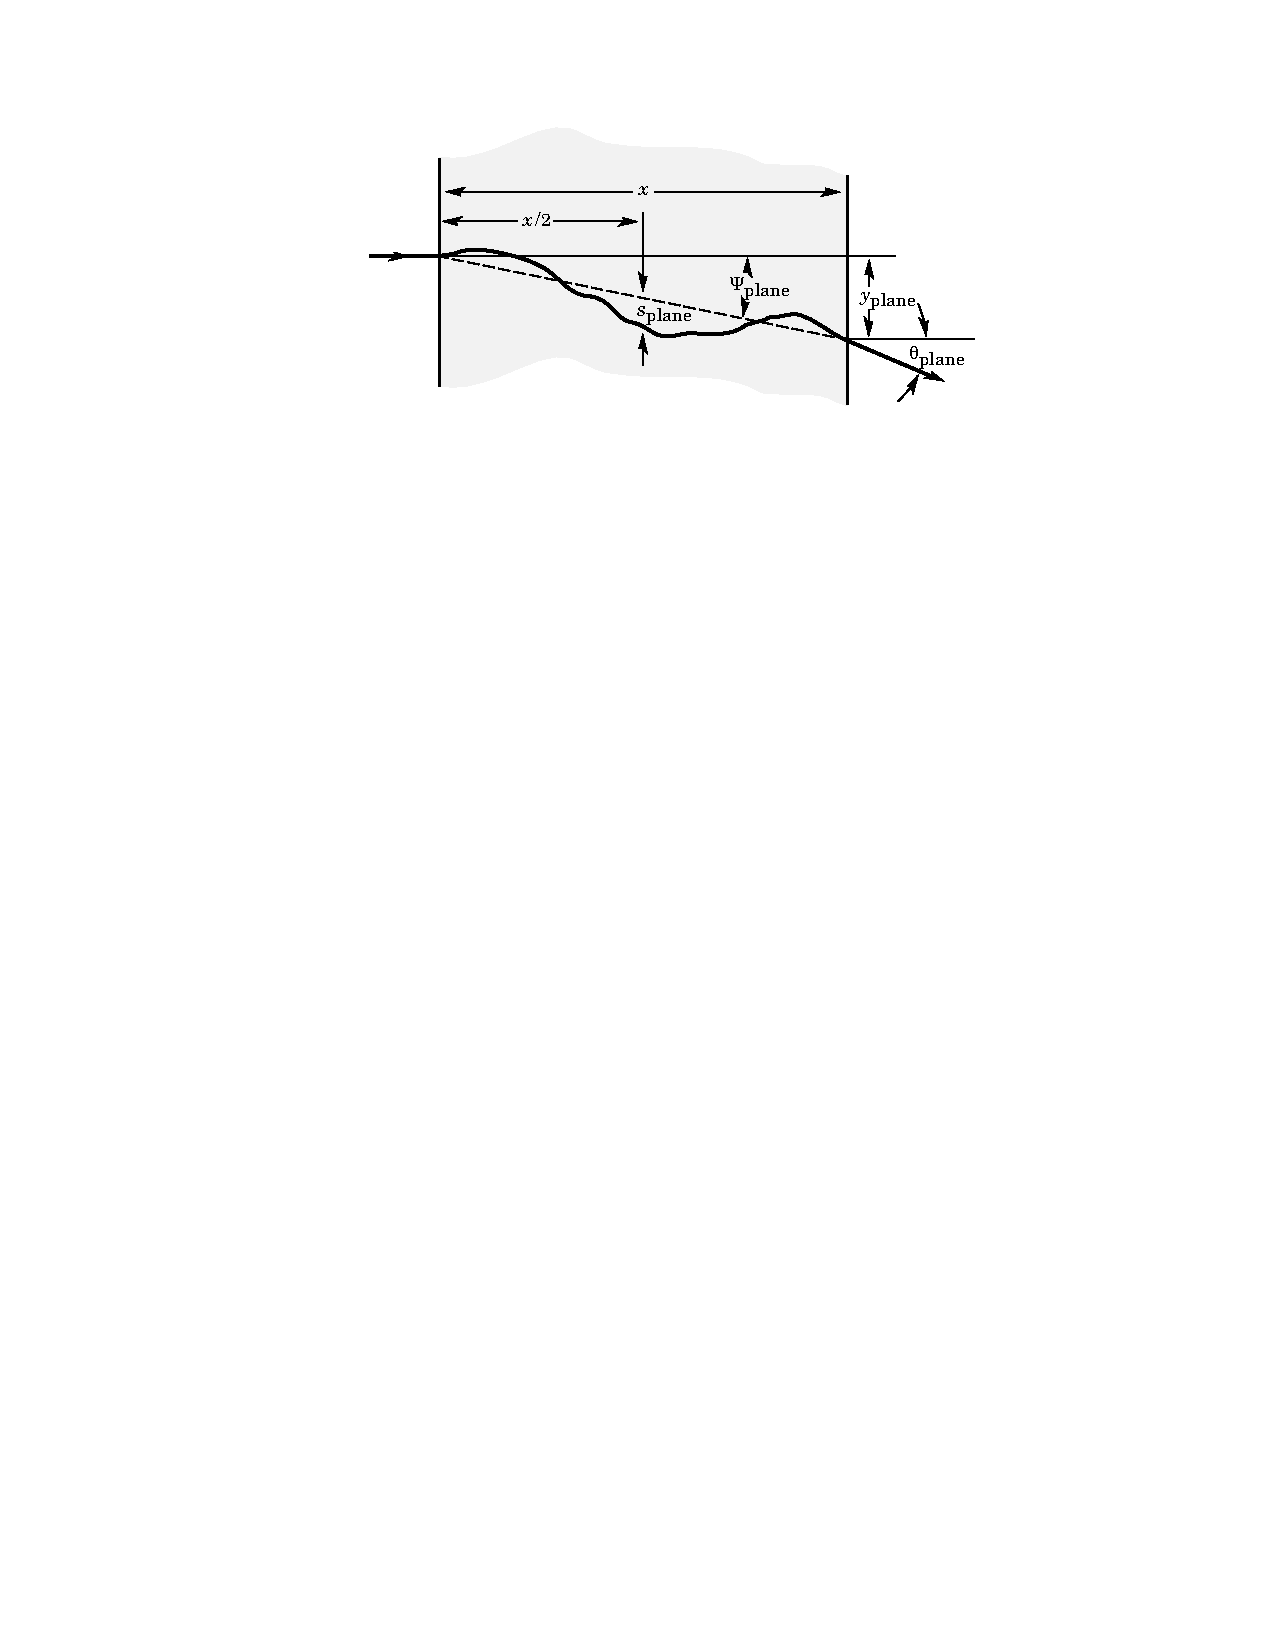
\includegraphics[width=0.95\textwidth]{fig/strongforce/matterinteractions/scattering_angle.pdf}
%%%\end{center}
%%%
%%%
%%%\paragraph{Particle Range: time permitting}
%%%The range $R$ of a particle is defined as the distance it will travel
%%%in the material before loosing all its energy through ionisation. It is a useful
%%%quantity, however it is not the full picture as particles can loose energy through
%%%other means, as we shall see later in the course.
%%%In any case it is interesting to calculate. 
%%%Suppose a particle enters a material with energy $E_0$. We can therefore define the range as
%%%\[
%%%<R>=\int_{E_0}^{0}\frac{dE}{<dE/dx>}.
%%%\]
%%%Insterting Eq.~\ref{eq:bethebloch}, we get 
%%%\begin{equation}
%%%<R>\propto \frac{E_{0}^{3/2}}{\sqrt{m}}.
%%%\end{equation}
%%%For the case when energy of incoming particle larger than the rest mass we have
%%%\[
%%%<R>\propto (\gamma m v)^{3/2}.
%%%\]
%%%
%%%\fbox{\parbox{0.98\textwidth}{
%%%\paragraph{Beyond scope:}
%%%So far we have discussed the average energy loss through ionisation $<\frac{dE}{dx}>$. In fact the actual energy loss scatters around the mean value ie
%%%\begin{center}
%%%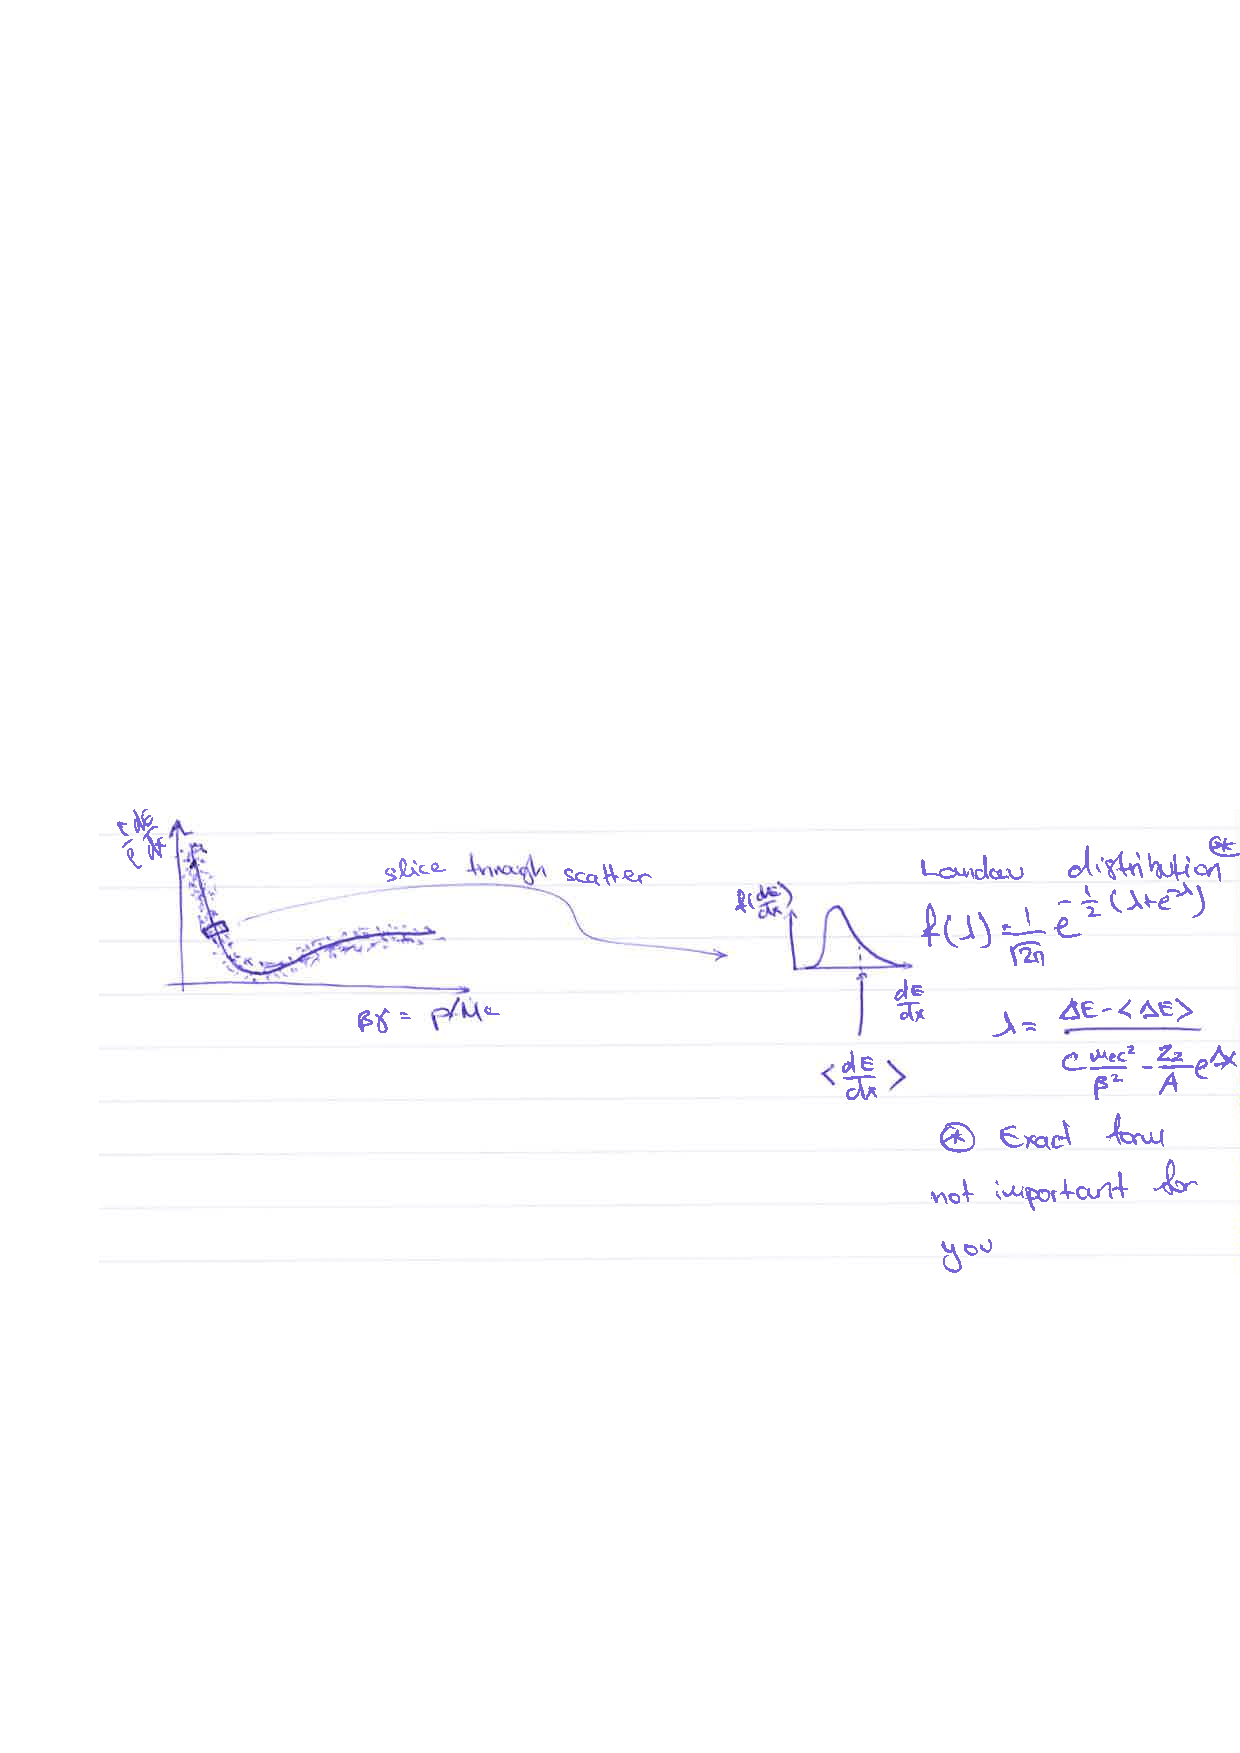
\includegraphics[width=0.95\textwidth]{fig/strongforce/matterinteractions/interactions3.pdf}
%%%\end{center}
%%%
%%%
%%%}}


\section{Particle accelerators and colliders}
This is a very quick overview of the most important types of particle
physics accelerators/colliders.

\begin{figure}[!h]
\centering
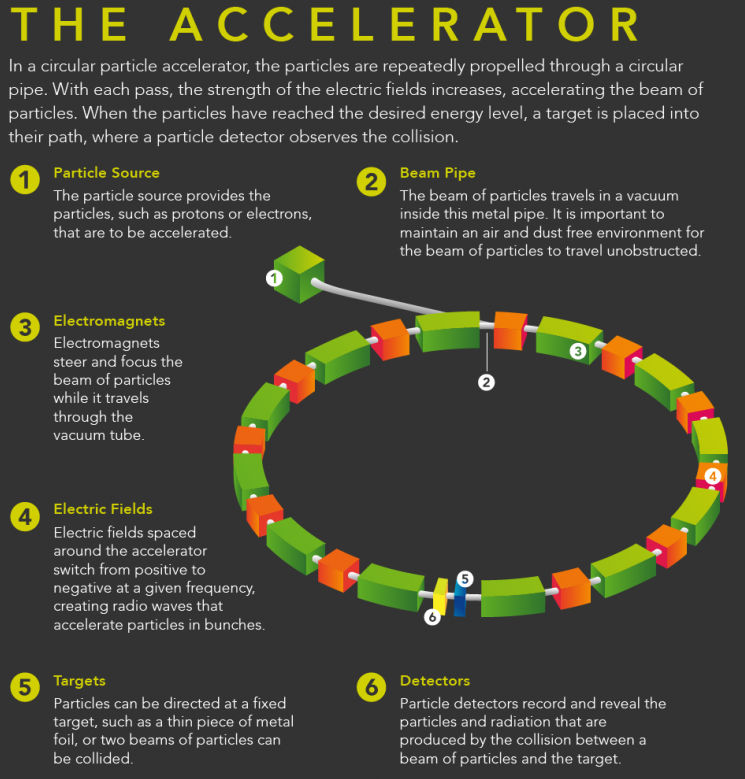
\includegraphics[width=0.9\textwidth]{fig/accelerators/0_CircularAccelerator}
\caption{A sketch of a circular accelerator with its basic components (from \href{http://energy.gov/articles/how-particle-accelerators-work}{http://energy.gov/articles/how-particle-accelerators-work}).
\label{fig:my_label}}
\end{figure}

\subsubsection{Circular versus linear}
There are two basic technologies: circular end linear accelerators. Circular accelerators have the advantage that one can give the accelerated particles a kick every time they come around, and also re-use those particles that did not disappear in the collision. They also allow a more compact design than linear accelerators. However, if one bends electrons or positrons around a circle (which is a type of acceleration) they loose a lot of energy through bremsstrahlung. This motivates the choice of linear accelerators for the next generation of very high energy electron-positron collider.

\subsubsection{Heavy particles for maximum energy}
The power $P$ of the bremsstrahlung emitted is proportional to $\gamma^4 = E^4/m^4$. For the same energy $E$, an electron looses $m_p^4/m_e^4 \approx 2000^4 = 16\cdot 10^{12}$ more energy than a proton. Therefore, protons can be accelerated to very high energies in a circular collider, without loosing significant amounts of energy through bremsstrahlung.
Proton colliders have therefore serious advantages for exploring the energy frontier (even though, as we shall see below, not all of the cm energy in proton collisions is available to produce new particles).

\subsubsection{Fixed target or collider? }
Once the particles have been accelerated, they need to be smashed into some target, or each other. In a fixed target experiment, the beam is dumped into some material. This is the technology of choice if the priority is to achieve high luminosities (high probability of some interaction is very high), and you don't care that you are colliding nuclei/protons (which are composite particles - see next section). The other option is collider experiment, where two beams are steered into each other. This is obviously much more challenging, and typically, only a few particles interact in each collision, so the luminosity is lower. But, as you learnt in the section on kinematics, far higher energies can be achieved this way, so if the purpose is to explore the energy frontier, you need to build a collider.

\subsubsection{Sledge-Hammer or scalpel?}
One of the most important differences between colliding protons with protons as in the LHC (or proton with antiproton as in the now decommissioned Tevatron), in contrast to electrons with positrons is due to the fact the electrons and positrons are fundamental particles, while protons are not.
\\\exercise{
Calculate the de-Broglie wavelength of a proton at the LHC in the cm system. How does this compare to the size of the proton?\vspace{2ex}\\
\rotatebox{180}{\parbox{0.95\textwidth}{$\lambda = \frac{h}{p}$ with $p=6.5TeV$ in the cm frame, and $h=2\pi \cdot 196\,\mathrm{MeV\,fm}$, $\lambda = 1.9\E{-4} \mathrm{fm}$, much smaller than the size of a proton of $\sim 1\mathrm{fm}$
}}}\\
At LHC energies (remember, high energies mean small distance scales), the proton is a complicated system of quarks and gluons. Each particle in this system is generically called a "parton". These partons are
\begin{itemize}
\item the valence quarks $uud$
\item gluons
\item sea quarks: quark-antiquark pairs that fleet in and out of existence. These are mainly light quarks $u\overline{u}$, $d\overline{d}$, and (less) $s\overline{s}$, but $c\overline{c}$ also plays a significant role.
\end{itemize}

\begin{figure}
\centering
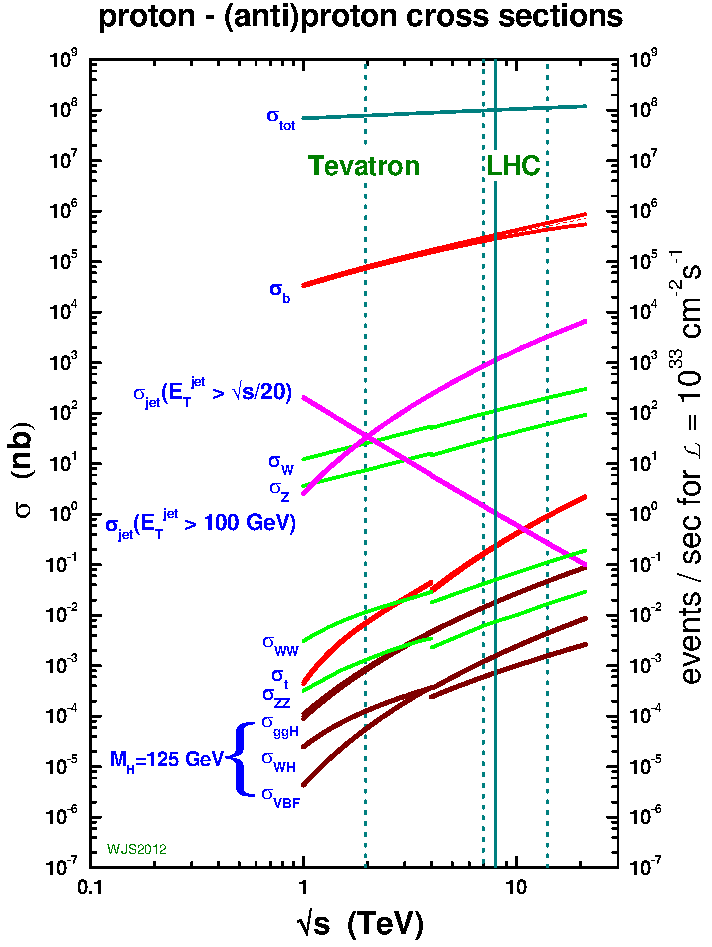
\includegraphics[width=0.7\textwidth]{fig/pp_xsection}
\caption{This plot shows the production cross section for $p\overline{p}$ (for $\sqrt{s}\le \un{4}{TeV}$) and $pp$ collisions (for $\sqrt{s} > \un{4}{TeV}$) as a function of the cm energy $\sqrt{s}$. Notice that the total $pp$ cross section is $10^{10}$ times bigger than that for Higgs production. The production cross section for $b\overline{b}$ is still $100,000,000$ time larger, meaning that the dominant Higgs decay mode $H \to b\overline{b}$ is completely drowned out by background. Note that one physicist's background is another physicist's signal: those huge numbers of $b\overline{b}$ events make LHCb the world-leading B-physics experiment.
From \href{inspirehep.net/record/810127?ln=en}{Eur.Phys.J. C63 (2009) 189-285} and \href{www.hep.ph.ic.ac.uk/~wstirlin/plots/plots.html}{www.hep.ph.ic.ac.uk/$\sim$wstirlin/plots/plots.html}.}
\end{figure}
At LHC energies the vast majority of the proton's energy is carried by gluons, so to first approximation, the LHC really is a gluon collider. The other big difference is of course that protons (and their constitutents) interact strongly, while electrons and positrons do not. Strong collisions tend to create far more particles in a collision.

\begin{figure}
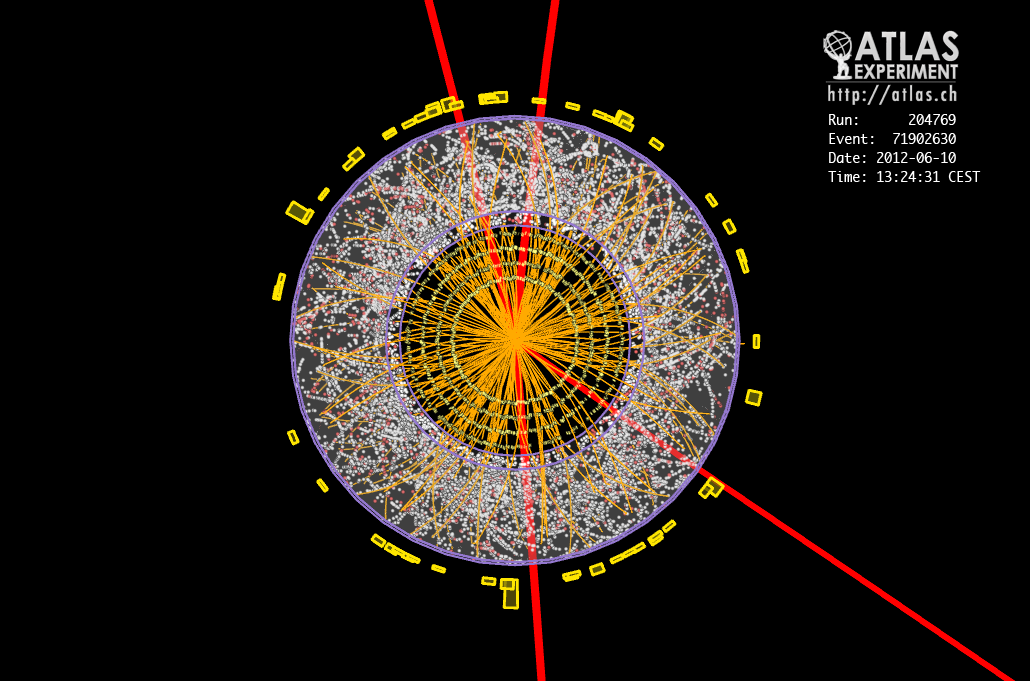
\includegraphics[width=0.58\textwidth]{fig/ATLAS_run204769_evt71902630}
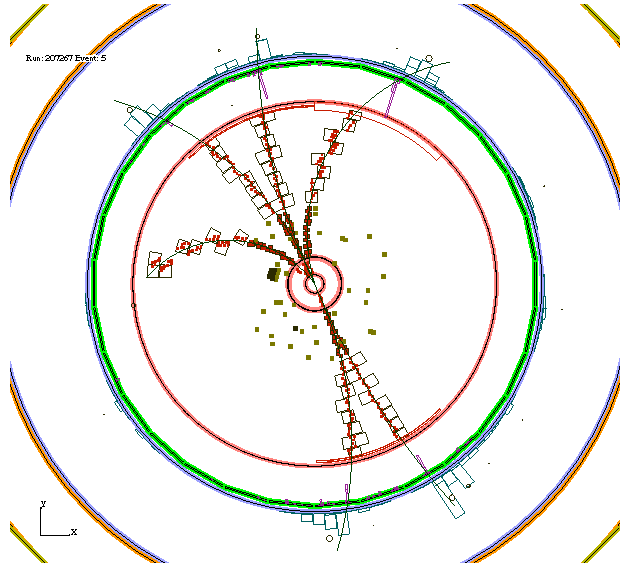
\includegraphics[width=0.4\textwidth]{fig/CLEOc_D2Kspipi_D2Kpi_Event}
\caption{Left: ATLAS event display for a p-p collision at the LHC. Two effects are compounded: The large number of track in each event, and the fact that that the LHC, multiple p-p collisions can happen in a single event. Right: CLEO-c event at an $e^+ e^-$ collider. Far fewer tracks are visible (in this case 6 tracks resulting from the process from $e^+ e^- \to \psi(3770) \to D\overline{D} \to (K_S\pi^+\pi^-)_D (K^+\pi^-)_{\overline{D}}$; the $K_S$ decayed to $\pi^+ \pi^-$) making reconstruction easier and cleaner.}
\end{figure}


The composite nature of the proton has the consequence that we do not know a priory what we are colliding. Most of the time, gluons, but with unknown momenta. 
This has the advantage that, at one proton collision energy, one can probe a wide range of gluon collision energies at the same time (good for discovery of unknown resonances/particles). 
It has the disadvantage that only some of the energy is available for the collision, and also that we do not know that energy, or the center of mass of the system. 

\subsubsection{Detecting invisible Particles}
\paragraph{Missing momentum in $e^+ e^-$ colliders}
\begin{figure}
\centering
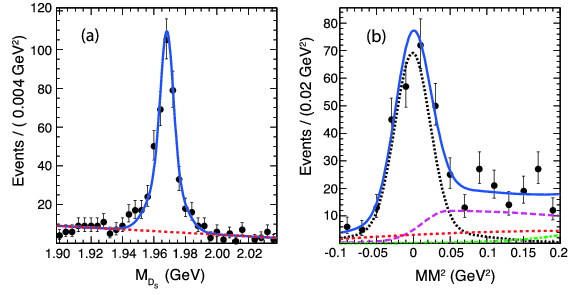
\includegraphics[width=0.9\textwidth]{fig/CLEO_Ds2munu}
\caption{Two plots from the reconstruction of \prt{D_s^+ \to \mu^+ \nu_{\mu}}: Left: the reconstructed mass-squared of the \prt{D_s} meson. Right: The reconstructed mass of the neutrino, inferred from the missing 4-momentum. The various lines show different contributions to the fit, with black-dotted signal, and the others different backgrounds (most prominently \prt{D_s^+ \to \tau^+ \nu_{\tau}} in pink-dashed). This clean reconstruction of invisible particles is only possible when the initial 4-momentum is known, as in an $e^+ e^-$ collider.
From: \href{https://inspirehep.net/record/810661/}{Phys.Rev. D79 (2009) 052001} \href{https://inspirehep.net/record/810661/}{[arXiv:0901.1216]}
\label{fig:CLEO_Ds2munu}}
\end{figure}

In electron-positron colliders, if one invisible particle (like a neutrino, or perhaps a dark matter particle) leaves the detector un-detected, we can still reconstruct its energy and momentum because we know the energies and momenta of the initial state and the other particles (see for example \figref{fig:CLEO_Ds2munu}. This is not possible at proton-proton collider. 

\paragraph{Missing transverse momentum (or $E_T$) in $p-p$ colliders}
\label{sec:missingEt}
\begin{figure}
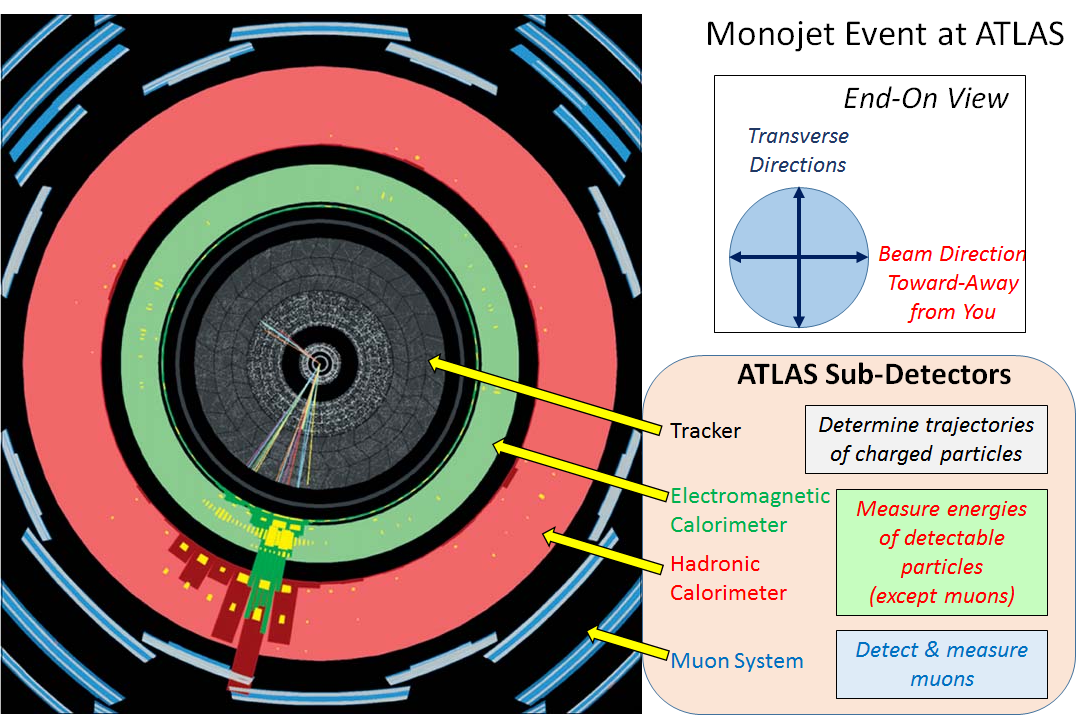
\includegraphics[width=0.52\textwidth]{fig/ATLAS_pp2nunuj_atlas}
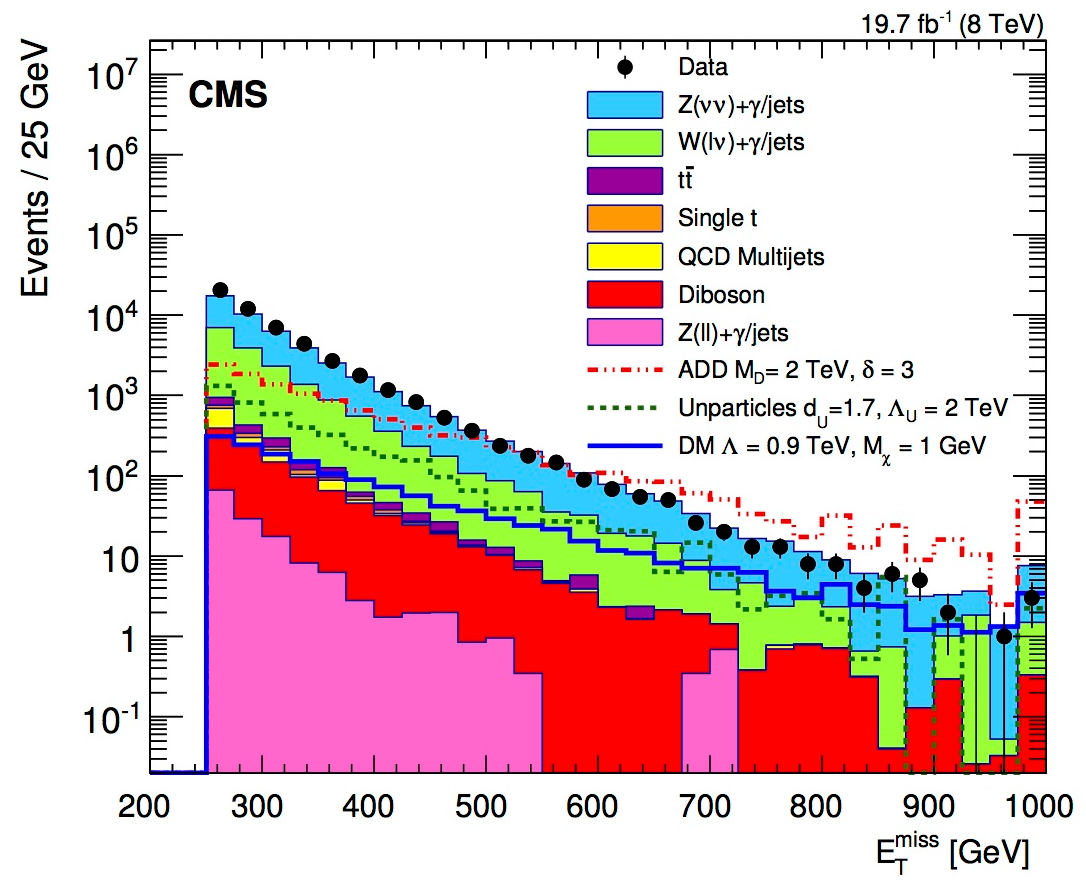
\includegraphics[width=0.45\textwidth]{fig/CMS_missingEtSpectrum}
\caption{Left: Event display from ATLAS (only showing high-energy tracks) with large missing $E_T$.
Right: Search for invisible heavy particles at CMS. The stacked coloured histograms correspond to missing $E_T$ signals from known standard model processes. The black dots represent the data. The dashed line corresponds to the signal expected in a certain New Physics model. Unfortunately, no new physics was seen, here.
\label{fig:missingET_atLHC}
}
\end{figure}

However, we can still do something even at proton-proton colliders: we know that the cm system has no transverse momentum, so the momenta perpendicular to the beam line mucht add up to zero. Often this is called transverse energy, $E_T$ but what is really meant by this is the magnitude of the \emph{vector} sum the momenta transverse to the beam direction:
\begin{equation}
E_T = \left|
\sum\limits_{\mathrm{i=all\;particles\;in\;collision}} \vec{p}_{Ti} \right|
\end{equation}
where $\vec{p}_{Ti} = (p_{ix}, p_{iy}, 0)$ is the transverse momentum of the $i$th particle and $z$ is the direction along the beam line. This needs to add up to zero if all particles have been detected. If it doesn't, we know that some particle has escaped undetected.

The complicated structure of the colliding protons, and the fact that they are made from strongly interacting particles, also results in the creation of a lot of particle jets in addition to creation and decay of the particles of interest (like the Higgs). 
The Higgs discovery is actually a nice example to illustrate the challenges (as well as the success) of the doing particle physics at hadron colliders: 
It is for these challenges, that the Higgs was not detected in its dominant decay mode, \prt{H \to b\overline{b}}. In the strong interaction processes at the LHC's proton-proton collisions, lots of $b\overline{b}$ quark pairs are produced, so the background to \prt{H \to b\overline{b}} is overwhelming. 
(BTW, the LHCb experiment uses this exact feature as its advantage and studies these huge quantities of $b\overline{b}$ quarks, and the mesons and baryons they form, for high precision flavour physics (i.g. \cpv) measurements.) 
The next heaviest pair of particles the Higgs can decay to is $\tau^+\tau^-$. But that is also really difficult to reconstruct, because the decay of each $\tau$ involves at least one neutrino (difficult, because we have no way to fully reconstruct its energy/momentum) and a virtual $W$. That $W$ can then either decay to leptons (which means more neutrinos, i.e. missing energy) or to jets (lots of background from QCD processes). 
At the end, the main discovery channels for the $H$ were \prt{H \to \gamma \gamma} (which proceeds via a loop diagram) and \prt{H \to 4\ell} ($\ell$ stands for $e^+$ or $e^-$ or $\mu^+$ or $\mu^-$) via an intermediate state of two $Z$ bosons (one virtual, one 'real'). 
Both of these are fairly rare, but "easy" to see, because they don't involve invisible particles, and they don't involve hadrons (strongly interacting particles) in the final state, and thus there is less background from all the QCD processes that go on in a hadron collider.

\subsubsection{Summary: $e^+ e^-$ vs $pp$}
The advantage of an electron-positron collider is then that the initial state is very well known, and the interaction is "clean", i.e. has less background. And if one knows where to look, one can tune the collider to the appropriate cm energy. It's ideal for precision studies. 
Therefore people are proposing to build a $e^+\,e^-$ collider (either circular or linear) to study the Higgs, and possibly (if the LHC finds any evidence for it), new particles beyond the SM. 
While for studying the Higgs, it is unclear if a linear or a circular collider is better, studying heavy new particles with masses in the TeV range would require a linear collider - circular ones would loose too much energy through bremsstrahlung to reach this energy. On the other hand, if we wanted to search for new heavy particles beyond the energies currently reached by the LHC, the best choice for achieving such high high energies is a proton-proton collider.

\exercise{In what way would a muon collider be the "ideal" collider? Why haven't we built one?}
 
\newpage

%% Week 7

\section{Weak Interactions}

\subsection{Discovery}
 In 1896 Henry Becquerel discovered that uranium crystal blacken
 photographic film if they are brought in close contact with
 it. Subsequently, Becquerel, Kaufmann and Rutherford show that
 uranium ore, like some other materials, emits fast, electrically charged
 rays, so-called $\beta$ radiation.

 These were electrons from the decay of protactinium
 \chem{\mbox{}^{234}_{91}Pa} to Uranium \chem{\mbox{}^{234}_{92}U}. 

 It was first assumed that the electrons emitted were in the atomic
 nucleus before the decay, but this did not agree well with the
 nuclear model (Rutherford 1909, and Bohr 1913), according to which
 the electron orbits were predominantly well outside the nucleus. With the
 discovery of the neutron by Chadwick it became evident that the
 electron is created when the neutron is converted to a proton.


\subsection{Non-Conservation of Energy}
 One of the most puzzling problems facing the early theory of neclear
 beta decay was the energy spectrum of the emitted electrons. The
 decay kinematics in $C\to A+B$ decays is quite simple the
 energy of the electron in the CM frame (which is usually also the lab
 frame) is
\begin{equation}
\label{eq:twoBodyEnergy}
E_A^{\mathrm{2-body}} = \frac{M_C}{2} + \frac{m_A^2 - m_B^2}{2M_C}
\end{equation}
 so the energy of the radiation in nuclear decay should be uniquely
 determined by the mass of the radiated particle and the masses of the
 relevant isotopes. And this is indeed the case for the other types or
 radio activity, coined at the time as alpha (He ions) and
 gamma (photons) radiation.
%
\begin{figure}
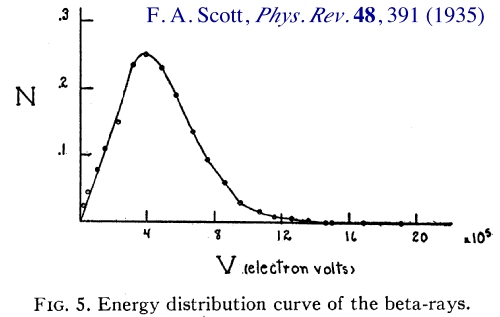
\includegraphics[width=0.5\textwidth]{fig/weak/betaspectrum.jpg}
\caption{Energy spectrum of $\beta$ rays in Radium A. A continuous energy
  spectrum up to the $E_e^{\mathrm{2-body}}$ is observed.
 \label{fig:betaEnergySpectrum}}
\end{figure}
 However, in 1930
 \href{http://www.nobel.se/physics/laureates/1935/chadwick-bio.html}{James
 Chadwick} discovered that, for beta radiation, this is not
 true. Instead energy spectra like the one in
 \figref{fig:betaEnergySpectrum} are observed, covering the entire
 kinematic range between $zero$ and the energy one would expect for 2
 body decays according to \eqref{eq:twoBodyEnergy}. One rather
 unattractive explanation for this observation would be the violation
 of energy conservation.

\subsection{Neutrinos}

 To rescue Energy conservation, Pauli proposed in 1930 the existence
 of an additional particle, that would carry the missing energy in the
 decay. This particle would have to be
\begin{itemize}
 \item neutral to escape detection
 \item very light or massless, to account for observed endpoints of
 the electron energy spectra i.e. the observation some that electrons
 seem to carry so much energy away that they leave nothing for the
 neutrino, not even for it to sit there if it has mass.
 \item spin \half, to account for angular momentum conservation.
\end{itemize}
 Initially he called this particle ``neutron'', but after the
 discovery of the neutron by Chadwick, he followed a suggestion by
 Fermi and named it neutrino.

\subsection{Fermi's theory of nuclear reactions}

 The original description, that worked well up to a certain energy, was Fermi's 4-point reaction: Have a
 neutron as the ingoing particle, the (lighter) proton outgoing, and
 instead of a photon, emit an electron-neutrino \emph{pair}.
\\
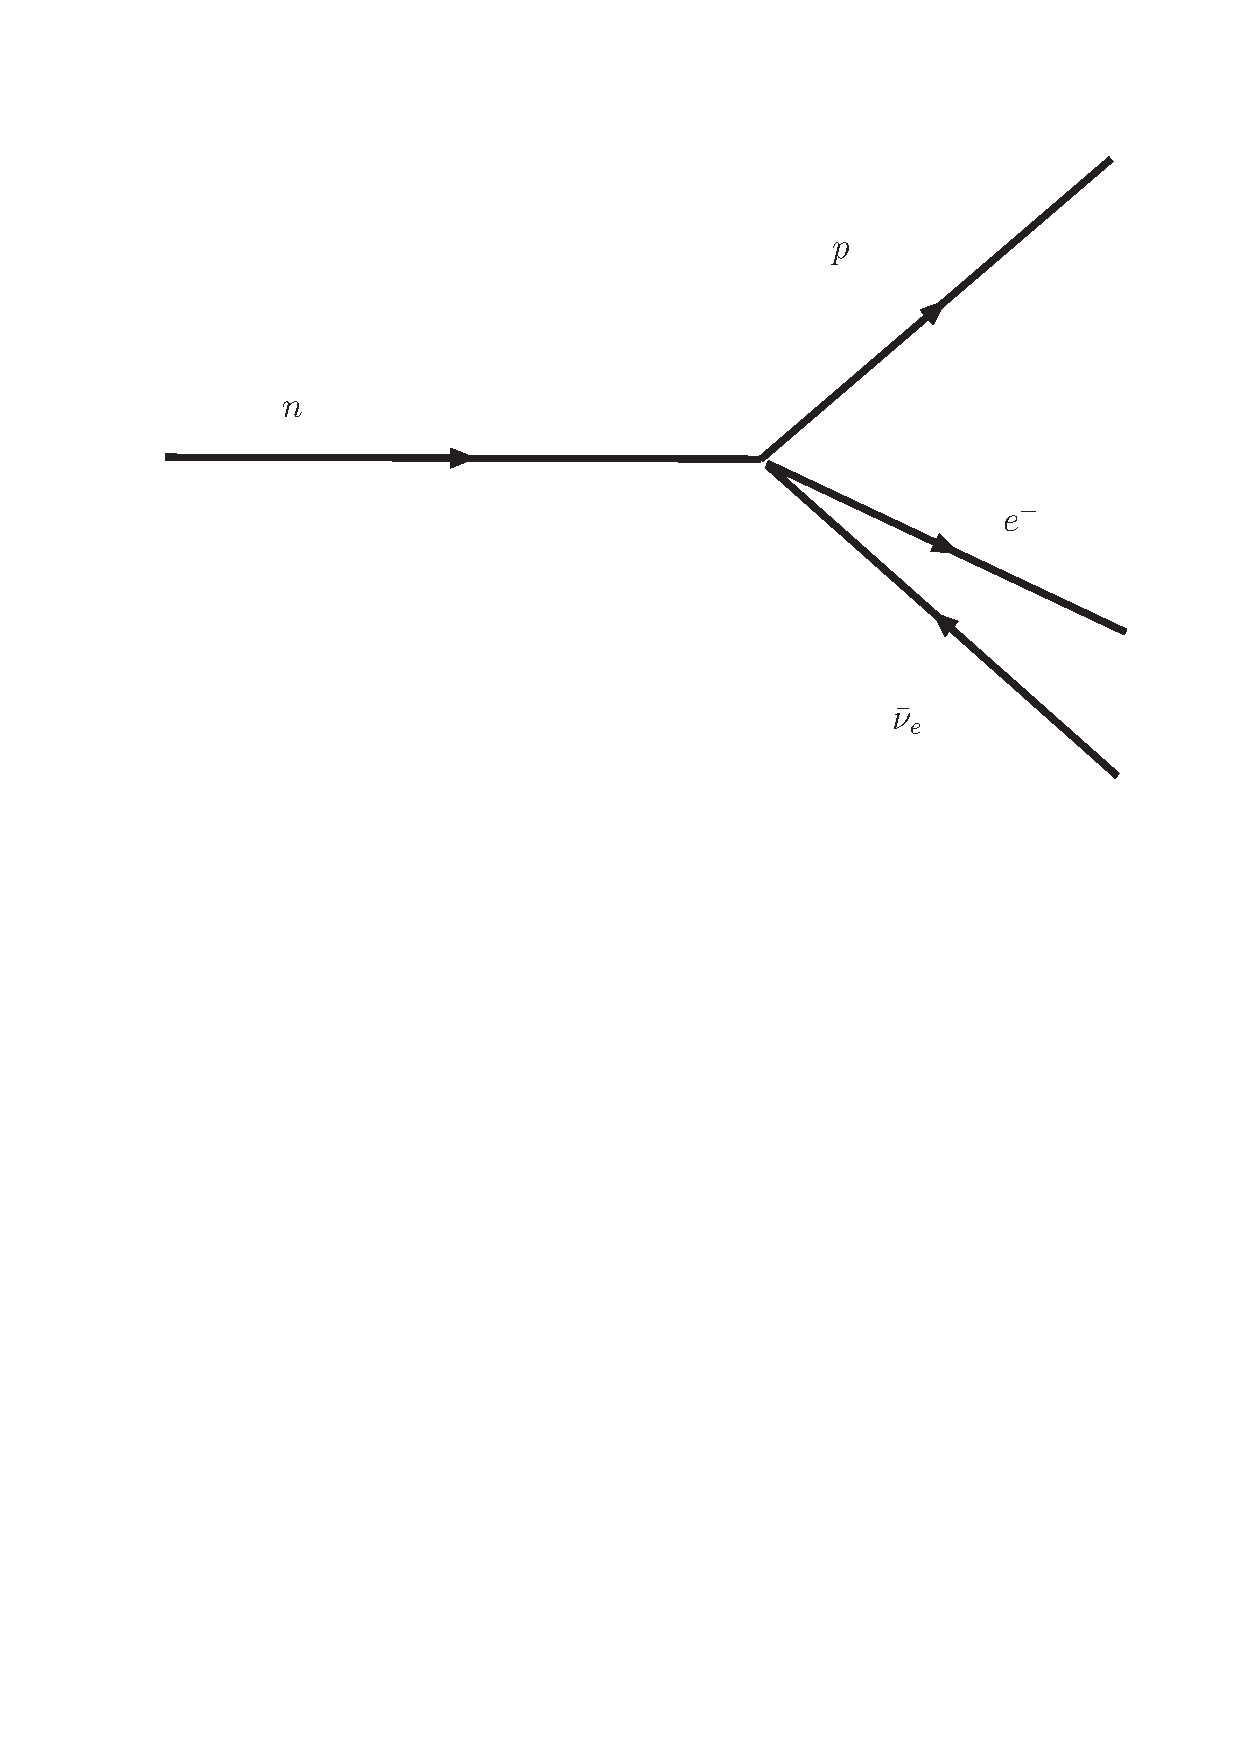
\includegraphics[width=0.5\textwidth]{fig/weak/fourPoing}
\\
The matrix elemement for that would simply be the vertex factor, which has a coupling strength of $\frac{G_F}{\sqrt{2}}$ ($G_F$ is known as "G-Fermi").

\subsection{Massive vector bosons}
Instead of a 4-point interaction, we describe this today as a $W$ exchange with vertex factor $g_w$. It leads to the same result as the Fermi fourpoint interaction for energies where $p^2 \ll M_W^2$ if we put $\frac{G_F}{\sqrt{2}} = \frac{g_W^2}{M_W^2}$. At energies with $p^2 \gg M_W^2$, we can neglect the $W$ mass and we get the same kind of behaviour as for a photon, however, with the electroweak coupling constant $g$ (which is actually larger than that of the photon). It's obvious that something will go wrong at $p^2 = M_W^2$, this can be avoided by changing the propagator to $\frac{1}{p^2 - M_W^2 + iM_W\Gamma_W}$ where $\Gamma_W$ represents the width of the $W$. We can usually leave it out since this is much smaller than $M_W$.
It's worth noting that people had identified strong theoretical reasons why the four-point interaction had to be modified before energies where it breaks down could be explored. 

\subsection{At this point, not all weak interactions were (yet) the same}
In fact, the picture above is a bit too simple. It was found that there are three different coupling constants. One for lepton vertices, that we call $g_W$ above and that applies to $e \nu_{e} W$, $\mu \nu_{\mu} W$, $\tau \nu_{\tau}W$ (although the $\tau$ was discovered later), one for the $ud W$ vertex (which is nearly $g_W$, but not quite) and one for the $usW$ vertex, which is much smaller.
Cabibbo had an ingenious idea how these three coupling constants could be unified. This described in the next section.

\section{Parity, and Parity Violation}
\subsection{Parity} 
 Parity, denoted by \ps, is the operation of replacing all space
 coordinates $x, y, z$ with $-x, -y, -z$, which is the effect of a mirror
 reflection followed by a \degrees{180} rotation.

 What we mean with parity symmetry is that the laws of physics should
 be symmetric. This means in practise that if you build an experiment
 with result x, then the mirror-reflected experiment should yield the
 mirror-reflected result.

 An example of a physical law that is symmetric under parity is
 gravity:
\begin{equation}
 m \frac{d^2 \vec{x}}{dt^2} = -G \frac{\vec{x}-\vec{y}}{|\vec{x}-\vec{y}|} 
 \frac{Mm}{|\vec{x}-\vec{y}|^2}
\end{equation}
 where $\vec{x}$ represents the position of some object with mass $m$
 (say earth) and $\vec{y}$ the position of another object with mass
 $M$ (e.g. the sun). Replace all co-ordinates with their negatives,
 i.e. \(\vec{x} \topar -\vec{x}\) and \(\vec{y} \topar -\vec{y}\) and
 the equation remains valid and the same. This is what's meant with
 parity symmetry. What matters is that the laws are invariant.  The
 fact that the two objects $m$ and $M$ find themselves in a different
 position after the parity operation does not violate parity. However,
 if they were now governed by different laws of physics, e.g. if they
 were suddenly not subject to the gravitational force anymore, that
 would violate parity. A thought experiment that would test for parity
 is to take two system, one the exact mirror image of the other. If
 the two evolve such that they remain exact mirror images of each
 other, parity is not violated. If they differ after a while, it is
 violated. 
 %Of course there are practical reasons why it is impossible to set up
 %experiments that are such exact mirror images that they'd remain
 %mirror images for all times, even if parity is not violated. This is
 %the sort of thing an experimenter will have to take into account
 %when evaluation the outcome of a real experiment, not a thought
 %experiment, though.

 Parity is a discrete symmetry, as opposed to a continuous
 symmetry. Continuous symmetry operations can be build up by a
 succession of infinitesimally small steps. Examples are, for example,
 rotations, and the associated conserved quantity is angular
 momentum. The conservation of such symmetries is very fundamental to
 our understanding of physics. Mirror reflection however is a discrete
 symmetry operation - there is no continuous path to transform an
 object into its own mirror image, you'll have to break it apart and
 build it from scratch. So, while a rotated object (or experiment) can be considered
 to be the same object as before the rotation, a mirror reflected
 object (or experiment) cannot, it is a different thing. This makes discrete
 symmetries fundamentally different from continuous ones, and there is
 clearly less reason to assume that they are good symmetries of
 nature.

 However, all physical interactions governing our every-day life are
 in fact mirror symmetric (gravity and electromagnetism) so the idea
 that parity is a fundamental symmetry of nature seems - well,
 natural. But, as we will see below, it is wrong. 

\subsection{The effect of parity on various quantities}

\paragraph{Position} That's how we defined it: 
\[ \vec{x} \topar -\vec{x} \]
\paragraph{velocity} Same thing, since $\vec{v} = \dbyd{}{t} \vec{x}$, so
\[ \vec{v} \topar -\vec{v} \]
\paragraph{mass} Remains the same - we \emph{define} the rest-mass as
 a property of the body, independent of its position.
\paragraph{momentum} of course the same as velocity
\[ \vec{p} \topar -\vec{p} \]
\paragraph{Energy} Remains the same. Intuitively clear, but also
 mathematically: Non-relativistically \( E = m\vec{v}^2 \), clearly
 invariant.  Similarly, relativistically, \(E = \sqrt{ m^2 +
 \vec{p}^2}\), also remains the same.
\[ E \topar E \]
\paragraph{angular momentum} More interesting:
\[ \vec{L} = \vec{r} \times \vec{p} \topar (-\vec{r})
\times (-\vec{p}) = \vec{r} \times \vec{p} = \vec{L},
\] so angular momentum is invariant under parity:
\[\vec{L} \topar \vec{L}\]
This is the defining property of an \textbf{axial vector}, or pseudo vector (while $\vec{x}$, $\vec{p}$ are simply vectors).
\paragraph{Electric field $\vec{E}$}
The electric field at $\vec{r}$ due to a point charge $q$ at the origin is:
\[
    \vec{E} = \frac{q}{4\pi\epsilon_0} \frac{\vec{r}}{|\vec{r}|}\frac{1}{|\vec{r}|^2}
\]
So 
\[
    \vec{E} \topar -\vec{E}  
\]
This can be more generically derived from Maxwell's equations, but for the purpose of these notes, we'll be satisfied with noting that
this remains true for a charge moving with speed $v$:
\[
    \vec{E} = \frac{q}{4\pi \epsilon_0} \frac{1-v^2/c^2}{(1-v^2\sin^2\theta/c^2)^{3/2}}
    \frac{\vec{r}}{|\vec{r}|}
    \frac{1}{|\vec{r}|^2}.
\]
\paragraph{Magnetic field $\vec{B}$}
The magnetic field due to a charge moving with velocity $\vec{v}$ is given by
\[
    \vec{B} = \frac{1}{c^2} \vec{v} \times \vec{E} 
\]
Since $\vec{v} \topar -\vec{v}$ and $\vec{E} \topar -\vec{E}$, we have
\[
    \vec{B} \topar \vec{B}
\]
So the magnetic field vector is an axial vector.
%%


\subsection{Parity in particle physics}
\label{sec:ParityInPP}
\subsubsection{Parity of individual particles}
Particles are described by a quantum mechanical wave function. How does this transform? This derives directly from the transformation properties of the parameters the wave function depends on, so in the position representation, we get:
\begin{equation}
    \psi(x, y, z) \topar \psi'(x, y, z) = \psi(-x, -y, -z)
\end{equation}
Because fundamental particles are point-like objects which have no structure of shape, they should be mirror-symmetric. Therefore, a fundamental particle at rest must transform into itself under parity.  For the wave function it means that
\begin{equation}
 \left|\psi \right|^2 \topar \left|\psi\right|^2
\end{equation}
Note that this is a relationship between the absolute squared of the wave-functions, which is the observable quantity. For the wave function this implies
\begin{equation}
 \psi \topar e^{i\phi} \psi
\end{equation}
 or equivalently
\begin{equation}
 \ps \psi = e^{i\phi} \psi
\end{equation}
This means that a wavefunction $\psi$ describing a single fundamental particle must be an eigenfunction of the parity operator \ps. Since $\ps^2=1$ (two mirror reflections = identity), $\ps^2$ has only one eigenvalue, which is $1$. Therefore \ps\ must have eigenvalues whose square is $1$. So the eigenvalues of \ps\ are $1$ and $-1$.
\begin{figure}
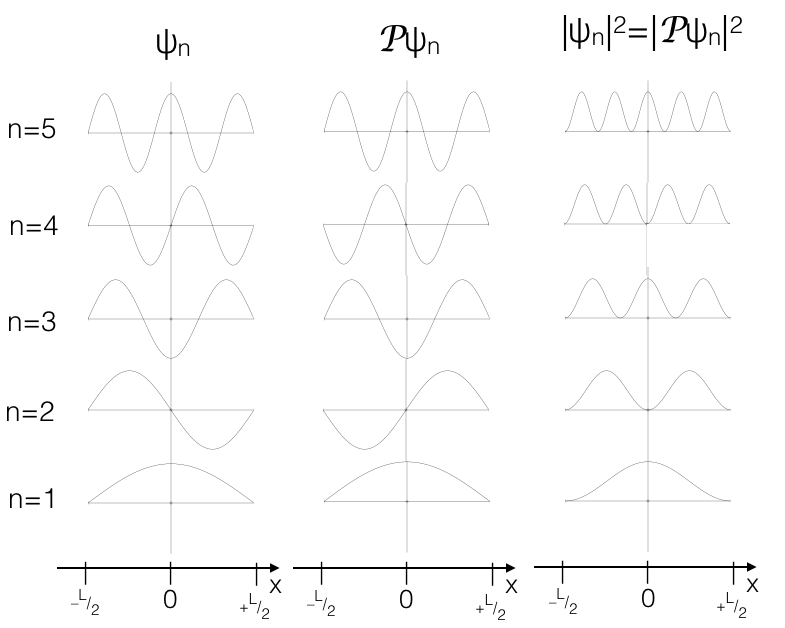
\includegraphics[width=0.9\textwidth]{fig/Parity_1D_squareWell}
\caption{The effect of parity on the wave functions describing a particle in an infinite square well of length $L$, in one dimension. The solutions to the Schr\"odinger equation are: $\psi_n(x)=\sin(n \pi (x/L + \half))$. The wave function $\psi_n$ is parity-odd (i.e $\ps \psi_n(x) = -\psi_n(x)$) for $n = 1, 3, 5 , \ldots$ and parity-even (i.e $\ps \psi_n(-x) = +\psi_n(x)$) for $n = 2, 4, 6, \ldots$. Note that in the analogy we use here, each $\psi_n$ corresponds to a different particle.
\label{fig:parity_1D_squareWell}}
\end{figure}
Let us have a look at a wave function of a particle in a 1-dimensional infinite square well, shown in \figref{fig:parity_1D_squareWell}. Because the square well is symmetric with respect to reflections about $x=0$, we require $|\psi_n(-x)|^2=|\psi_n(x)|^2$, which we do indeed find in the solution: $\psi_n(x)=\sin(n \pi (x/L + \half))$. The wave function $\psi_n$ is parity-odd (i.e $\ps \psi_n(x) = -\psi_n(x)$) for $n = 1, 3, 5 , \ldots$ and parity-even (i.e $\ps \psi_n(-x) = +\psi_n(x)$) for $n = 2, 4, 6, \ldots$. Note that in the analogy we use here, each $\psi_n$ corresponds to a different particle (rather than one and the same particle in a different energy states). In reality, particles move in 3 spatial dimension, and we demand symmetry about their own origin, i.e. $|\psi(x,y,z)|^2 = |\psi(-x,-y,-z)|^2$, leaving us with...\\
\fbox{\parbox{0.98\textwidth}{
 Two kinds of particle
 wavefunctions, one picks up a '$-$' sign under parity (parity odd), the other does not (parity even).
 }}
\begin{equation}
\begin{array}{rcrl}
 \psi& \topar & \psi & \mbox{even intrinsic parity}
\\
 \psi& \topar & -\psi & \mbox{odd intrinsic parity}
\end{array}
\end{equation}
 Both exist in nature. In the formula sheet at the back you find a list of particles, and for each the $J^{PC}$ quantum numbers are given. 
 $J$ is the spin of the particles. $P$ is its parity eigenvalue. The meaning of $C$ (which is not defined for all particles, in which case only $J^P$ is given), will be discussed very soon. 
 Looking at the quantities we know, we find that the $\pi^+$, for example, has $J^{P} = 0^-$, which means it is a spin zero particle which is parity-odd, i.e. has parity eigenvalue $-1$. The $f_0(980)$ has $J^{PC}=0^{++}$, so it is also spin zero, but parity-even (and it also as $C=+1$, but as mentioned previously, we learn about the meaning of that later). 
 You will not find a parity value for electrons, muons, etc. There you use instead the following rule:
 \fbox{\parbox{0.9\textwidth}{
 Fermions have
 always the opposite parity of their antiparticles, so fermion
 anti-fermion pairs (like $e^+ e^-$) always have combined negative intrinsic parity. (The full parity value of the system also depends on the angular momentum as described below.)
}}

 \subsubsection{Parity of a two-particle system}
 You are familiar with a very famous two-particle system from your quantum mechanics course, the Hydrogen atom. This can be solved by reducing it to a one-particle problem of an electron (with reduced mass) in a $1/r^2$ potential. The solutions in spherical coordinates are of the form
 \begin{equation}
  \psi(r, \theta, \phi) = f(r) Y^{m}_{L}(\theta, \phi)
 \end{equation}
 \begin{figure}
 \begin{tabular}{ccc}
 \parbox{0.4\textwidth}{\includegraphics[width=0.4\textwidth]{fig/Parity_sphericalCoord_before}}
& {\Huge \topar} &
 \parbox{0.4\textwidth}{\includegraphics[width=0.4\textwidth]{fig/Parity_sphericalCoord_after}}
 \end{tabular}
 \caption{Spherical Coordinates under Parity.\label{fig:sphericals_under_parity}}
 \end{figure}
 So it factorises in a part that depends on the radial distance $r$ described by $f(r)$, and in another that depends on the angles $\theta$ and $\phi$. That latter part is $Y^{m}_{L}(\theta, \phi)$, the spherical harmonic function labelled by the orbital angular momentum quantum number $L$ and the magnetic quantum number $m$. Spherical coordinates transform under parity like this (see \figref{fig:sphericals_under_parity}):
 \begin{eqnarray}
    r & \topar & r \nonumber\\
    \theta & \topar & \pi - \theta \nonumber \\
    \phi & \topar & \phi + \pi
 \end{eqnarray}
 So, under parity, nothing is going to happen to $f(r)$. For the spherical harmonic, it turns out
 \begin{equation}
  Y^{m}_{L}(\theta, \phi) \topar 
  Y^{m}_{L}(\pi-\theta, \phi+\pi)
  = (-1)^L Y^{m}_{L}(\theta, \phi)
 \end{equation}
 So $Y^{m}_{L}$, and hence the entire wavefunction describing the electron-nucleus system, is parity even for $L=0, 2, 4, \ldots$ and it is parity odd for $L=1, 3, 5, \ldots$. 
 
 
 The factorisation of the solution into an $r$-dependent part and a spherical harmonic, $\psi(r, \theta, \phi) = f(r) Y^{m}_{L}(\theta, \phi)$, is not specific to the hydrogen atom, it results directly from the symmetry of the problem and generalises to any two-particle systems composed of point particles (which is the approximation being made when you derive this for the Hydrogen atom).
 So we can generalise our observation to the sweeping statement: The parity of a two-particle system is $(-1)^L$ \emph{multiplied} with the intrinsic parity eigenvalues of the constituents. This result is so important, we repeat it in a box:\\
 \fbox{\parbox{0.98\textwidth}{
\paragraph{Key result: The parity (P) eigenvalue of a two body system}
If each particle is a P eigenstate.
\[
P = (-1)^{L} \times \prod\limits_{\mathsf{all\;particles}} \mbox{(intrinsic parity)}
\]
The intrinsic parity of a fermion-antifermion pair is $-1$, so, for a pair of spin-\half\ fermions $P =(-1)^{L+1}$. For a pair of pions, which each have intrinsics parity $-1$, the overall parity value is $P=(-1)^L$.
}}
So, for example two pions in an $L=0$ state have parity $+1$. Two pions in an $L=1$ state have parity eigenvalue $-1$. A pion and an $f_0(980)$ in a $L=0$ state have parity $-1$, etc.

\paragraph{Parity of three and more-body systems}
To calculate the parity of systems with more than two particles, we break down the problem into successive 2-body problem. So we group particles into pairs, calculating the parity of each pair, $P_i$, and then treat each pair as if it were a single particle with intrinsic parity $P_i$, and repeat until we have only two particles left. This is best explained by example. Consider $\pi^+ \pi^- \pi^0$.

Let us treat this as \prt{\pi^+ \pi^-} pair plus a $\pi^0$. The \prt{\pi^+ \pi^-} pair has intrinsic $P_{1\,\mathsf{intrinsic}}=(-1)\cdot(-1)=+1$. Let us assume that the $\pi^+ \pi^-$ system has angular momentum quantum number $L_1$. Then its total parity of the $\pi^+ \pi^-$ system is $P_1 = (-1)^{L_1} \cdot (+1)=(-1)^{L_1}$.

The intrinsic parity of the \prt{\pi^0} is $-1$. Let's call the angular momentum of the $\pi^0$ relative to the \prt{\pi^+ \pi^-} pair $L_2$. Then the total parity of the three particle system is $P = P_1 \cdot (-1) \cdot (-1)^{L_2}= (-1)^{L_1 + L_2 + 1}$
To evaluate $P$ from this, we need to know something about $L_1, L_2$. Usually we do now know $L_1$, $L_2$ individually, but we do know the total angular momentum of the system.

Let us first consider the case where the three pions result from the decay of a spin zero particle, as in \prt{D^0 \to \pip\pim\piz}. Then the total $L+S$ of the three pion system must be $0$. Because the pions all have spin $0$, $L=0$. For a given pair of values $L_1, L_2$, the total angular momentum of the system, $L$, can have values 
$L = |L_1 - L_2|, \ldots, L_1 + L_2$. So $L=0$ is only possible if $L_1 = L_2$. Hence $P =  (-1)^{2L_1 + 1} = -1$

The situation is more complicated with a three pion system with overall $L=1$ (which is what we could get if it results from the decay of a spin-1 particle), which can have different parities, depending on the relative angular momenta between the particles that make up the overall $L=1$ state. For example, the \prt{\pi^+\pi^-} system could be in an $L_1 =1$ state. Then the relative angular momentum between the \prt{(\pi^+\pi^-)} system and the \piz\ can be $L_2 = 0, 1, 2$ without violating angular momentum conservation. The parity of the system is even for the $L_2 = 0$ and $L_2 = 2$ case, and odd for the $L_2 = 1$ case.

(In contrast to last year, you will not be asked to calculate the parity of three or more body systems in the exam with an initial state with $J=1$, but you should still know the basic ideas and results.)

\subsection{Parity Symmetry and Conservation}
 As you will remember from Quantum Mechanics, every symmetry comes
 with a conservation law. If parity were a good symmetry, it would
 imply that the commutator between the Hamiltonian that describes our
 parity-symmetric physics, and the parity operator, vanishes.
\begin{equation}
 \left[\ps, H\right] = 0
\end{equation}
 This has two consequences for a conserved symmetry:
\begin{itemize}
 \item If \ps\ is a good symmetry it can be measured simultaneously
   with energy/mass, so \ps\ is a good quantum number and for any
   particle one should be able to measure both its parity and its mass.
 \item If \ps\ is a good symmetry parity would be conserved, i.e. if a state is
 parity even, it will always remain parity even (even after a particle decay, for example), and if a state is parity odd, it will always parity
 odd. A parity odd unstable particle would always decay to a parity
 odd final state, a parity even one always into a parity even final
 state.
\end{itemize}

If parity is a good symmetry of nature, parity must be conserved in particle decays. To decide if a particle decay conserves parity we need to evaluate the parity before and after the decay. For this, we need to consider the parity eigenvalues given in the formula sheet, and we need to figure out the possible angular momentum states of any multi-particle system.

\paragraph{Example}
Let us consider $f_0(980) \to \pi^+ \pi^-$. The parity of the initial state is given to us in the formula sheet. For the $f_0(980)$ we find $J^P = 0^+$ (where $J=$spin and $P = \pm$ for parity even/odd), so it is parity-even. The $J^P$ of the pions is $0^-$. 
To evaluate the parity of the final state we need to know the angular momentum. Because $\vec{L}+\vec{S}$ is conserved, and all particles involved have spin ($J=0$), $L$ must be zero. So the parity of the final state is
\[
P = (-1)^{0} \times (-1) \times (-1) = +1
\]
which is the same as the initial state. Hence Parity is conserved in this decay.

\paragraph{Example}
Let us consider $K^+ \to \pi^+ \pi^0$. For the \prt{K^+}, $J^P = 0^-$, so the parity of the initial state is $-1$. The $J^P$ of the pions is $0^-$.  The $\eta$ has spin $J=0$, as do the pions, therefore, due to angular momentum conservation, $L$ must be zero. So the parity of the final state is
\[
P = (-1)^{0} \times (-1) \times (-1) = +1
\]
which is not the same as the initial state. Hence Parity is violated in this decay.

\paragraph{Example}
Consider $\rho \to \pi^+ \pi^-$. The $\rho$ had $J^P=1^-$. So it is parity odd. The pions have $J^P=0^-$, so they are each parity odd. Because the $\rho$ has $J=1$ and the pions have each $J=0$, the angular momentum quantum number of the two-pion system must be $L=1$. Hence the final state parity is:
\[
P = (-1)^{1} \times (-1) \times (-1) = -1
\]
which is the same as the initial state. Hence Parity is conserved in this decay.

\paragraph{Example}
Consider $D^0 \to \rho^+(770) \rho^-(770)$. The \prt{D^0} has $J^{P}=0^-$. So it is parity-odd. The $\rho$ mesons have $J^P=1^-$. Because each $\rho$ has $J=1$, they can combine to a total spin of $S=0$, $1$, or $2$. Because the inital state was $J=0$, the angular momentum needs to compensate for the spin, leading to $\vec{L}+\vec{S}=0$. This means $L$ can be either $0,1,2$.
\[
P = (-1)^{L} \times (-1) \times (-1) = (-1)^L
\]
Depending on $L$, the final state is therefore either parity odd ($L=1$) or even ($L=0,2$). This means that (if we don't know $L$), the observation of this decay would be compatible with parity conservation, as the final state can have the same parity as the initial state.

Parity conservation was the assumed to be true
 for a long time. Then came the $\tau-\theta$ puzzle, and eventually Wu's experiment. But let's first practice our parity violation detection skills:\\
\exercise{\textbf{Parity violating decay or not?}
For the following decays, decide whether the decay violates parity or not. You can find the spin and parity eigenvalues of the particles involved in the formula sheet in the format and $J^P$ where $J$ is the spin, and $P$ indicates whether it's a positive ($+$) or negative ($-$) parity eigenstate. For particles that are their own antiparticle you find two signs in the exponent, $J^{PC}$ - see \secref{sec:ChargeConjugation} for the meaning of $C$, you don't need it for this question.
%%
\begin{enumerate}[i)]
\item \label{parq1} \prt{K^{*0} \to K^+\pi^-}
\item \label{parq2}\prt{f_0(980) \to \pi^+ \pi^-}
\item \label{parq3}\prt{D^0 \to K^+ K^-}
\item \label{parq4}\prt{\phi \to K^+ K^-}
\item \label{parq5}\prt{J/\psi \to \mu^+ \mu^-}
%\item \label{parq6}\prt{D^+ \to K^-\pi^+\pi^+}
\item \label{parq7}\prt{\Do \to \pi^+\pi^-}
%%\item \label{parq8}\prt{\omega(782) \to \pi^+ \pi^- \pi^0}
\item \label{parq9}\prt{\eta \to \pi^+ \pi^-}
\end{enumerate}
\rotatebox{180}{Answers: \ps\ conserving are~\ref{parq1},\ref{parq2}, \ref{parq4}, \ref{parq5}, %\ref{parq6}
%, \ref{parq8}
. The others violate \ps\ symmetry.}
}
\\

%% \subsection{The $\tau-\theta$ puzzle*}
%% It was observed the \prt{K^+} meson (which has spin 0) can decay to two as well as three
%% pions. In \secref{sec:ParityInPP} we found that a $L=0$ system with 2 pions has positive parity, while a system of $3$ particles with a total $L=0$ has negative parity. This means that the
%% \prt{K^+}, which must be a parity eigenstate (at least if parity is conserved, because then $[H,\ps]=0$ and mass [energy] eigenstates are parity eigenstates), can decay to both, positive and negative parity states,
%% which violates parity conservation. At the time, it was firmly
%% believed that parity must be a good symmetry of nature. It was
%% therefore suggested that there are in fact two distinct particles,
%% the $\tau$ and the $\theta$, with different parity, which happen to
%% have exactly the same mass (this idea is not soo outlandish, given
%% that for example the $\rho^0$ and the $\omega$ are two different
%% particles with nearly the same mass). However T.~D.~Lee and
%% C.~N.~Young\footnote{T.~D.~Lee and
%% C.~N.~YoungPhys.~Rev~{\bf~104},~254~(1956)} pointed out that there is
%% actually no reason to assume parity conservation, that no data
%% existed that contradicted parity violation in weak interactions, and
%% that the assumption of parity violation in weak interactions would
%% solve the $\tau-\theta$ puzzle.




%\subsection{Cabibbo Angle}
 It was found that the 
 theory of weak interactions explained well many features of quark and
 of leptonic decays. However, it appeared that the interaction
 strength in quark decays was less than one would expected, especially
 the strange quark seemed to be very reluctant to decay.

 To solve this problem, Cabibbo proposed that the down and the strange
 quark ``share'' the interaction strength/transition amplitude to the
 up quark \cite{cabibbo}. The idea is that there is a particle
 \emph{like} the down quark (let's call it $d^{\prime}$) that couples
 with the expected strength to the up quark, but is in fact a
 superposition of the physical $d$ and $s$ quark.
 \begin{equation}
     d^{\prime} = \alpha d + \beta s
 \end{equation}
 Normalising the $d^{\prime}$ wave function leads to the condition that $\alpha^2 + \beta^2=1$. This is fulfilled by:
 \begin{equation}
 d^{\prime} = \cos\theta_C \, d + \sin\theta_C s
\end{equation}
where $\theta_C$ is the Cabibbo angle (experimentally $\theta_C = 0.22$).
In this scheme, a $d^{\prime}, u, W$ vertex has the same coupling strength ($g_W$) as an $e, \nu_e, W$ vertex. 
But in reality, we do not observe $d^{\prime}$, but the physical $d, s$ quarks ("physics" meaning that they have well defined masses. 
The amplitude for a $d^{\prime}$ become a $d$ quark is $\braket{d^{\prime}}{d} = \cos\theta_C$. Similarly $\braket{d^{\prime}}{s} = \sin\theta_C$.
 So the transition amplitude for $d \to u$ transitions is $\propto
 \cos\theta_C$ and for $s\to u$ transitions it is $\propto \sin\theta_C$
 (Remember that rates are $\propto |\mathrm{amplitude}|^2$).
 
\begin{figure}
\caption{The Cabibbo Angle.\label{fig:cabRot}}
\begin{tabular}{cc}
\parbox{0.45\textwidth}{
The down-type quarks that couple via the $W^{\pm}$ to the up-type quarks are rotated relative to their mass
eigenstates.}
&
\parbox{0.45\textwidth}{
The $W^{\pm}$ can induce a transition $u\to d'$. The transition amplitudes to the mass eigenstates $d, s$  are $\propto$ the
projections of the mass eigenstates onto the $d'$.
}
\\
\includegraphics[width=0.45\textwidth]{fig/C_P_CP/cabibboAngle.png}
&
\includegraphics[width=0.45\textwidth]{fig/C_P_CP/cabbibo_with_su.png}
\end{tabular}
\end{figure}
 For symmetry reasons, let us also define an $s'$ such that $d', s'$ are simply rotates states of $d, s$ (this is somewhat anticipating the addition of the charm quark below - an $s'$ doesn't really make sense unless it is the partner of 2nd up-type quark):
 \begin{equation}
   \label{eq:dprime_sprime_trans}
\vII{d^{\prime}}{s^{\prime}} = \mII{\cos\theta_C}{\sin\theta_C}
                                  {-\sin\theta_C}{\cos\theta_C}
\vII{d}{s}
\end{equation}
as illustrated in \figref{fig:cabRot}.

The introduction of quark mixing explained the observed
 $s\leftrightarrow d$ and $u \leftrightarrow d$ couplings, and related them to $W^{\pm}$ couplings in the lepton sector.
 
 So the vertex factors are now:\\
 \includegraphics[width=0.5\textwidth]{fig/weak/gWCabibbo}
 
 So instead of three coupling constants, we have one coupling constant
 $g_W$ and one angle, $\theta_c \sim 13.02^{\circ}$ - that is one
 fewer parameter. Describing nature with fewer parameters is usually a
 sign of progress in our understanding of it.
 
 Note that, while $u \leftrightarrow s$ and $u \leftrightarrow d$
 transitions are allowed, no vertices for $s \leftrightarrow d$
 transitions are allowed (even though there is a neutral $Z$ boson
 that could take care of the charge conservation). This is explored a
 bit more deeply in the Appendix~\ref{sec:tree_fcnc}.

\section{New Physics in 1963: Discovery of charm}
 (1963, quarks known at the time: $u, d, s$)\\ In the previous
chapters you learnt about the evidence for the existence of three
quarks, which beautifully described the otherwise messy picture of the
mesons and baryons observed. The key aspects of the theory of weak
interactions (that you also learnt about last year), were also
developed at a time when only three quarks were known: $u, d, s$. The
4th quark, charm, was predicted from observations made in decays of
Kaons. Note that this is quite remarkable. Kaons have a mass of less
than \un{0.5}{GeV}, while the charm quark has a mass of \un{1.3}{GeV}
-- so how can you see a charm quark in a Kaon decay? With this
section, we introduce an important general principle of an approach
that is called "flavour physics": The discovery of "new physics" at
mass scales beyond those of the particles that can be directly
produced and observed, using precision measurements.


\subsection{Flavour changing neutral currents at loop level}
\begin{figure}
\centering
\includegraphics[width=0.9\textwidth]{fig/0_K2mumu1}
\caption{Diagrams contributing to the "Flavour Changing Neutral Current" (FCNC) transition \prt{K^0 \to \mu^+ \mu^-} (w/o GIM cancellation) leading to predicted rates far higher than observed. It is an FCNC because it is a $d-s$ annihilation, so a $d$ couples (indirectly) to an $s$ which has the same charge.
\label{fig:K2mumu1}}
\end{figure}
 The theory as it stands now has one substantial problem suffered from
 one problem, and that was the prediction of ``Flavour Changing
 Neutral Currents'', or FCNC, transitions where the quark flavour
 changes, but not the charge, like $d\to s$.  With the advent of the
 Standard Model of particle physics we know these were already
 impossible at tree level, but loop diagrams such as those in
 \figref{fig:K2mumu1} for the process \prt{K^0 \to \mu^+\mu^-} are
 still possible. This had never been seen and the predicted rate for
 this process was far greater than the observed limits at the time.
 

\subsubsection{GIM}
\begin{figure}
\centering
\includegraphics[width=0.9\textwidth]{fig/0_K2mumuGIM}
\caption{GIM mechanism illustrated for the "Flavour Changing Neutral Current" transition \prt{K^0 \to \mu^+\mu^-}. The diagrams resulting from the newly predicted $c$ quark exactly cancel the diagrams with the $u$ quark in the loop. Well - nearly exactly. The mass difference between the $c$ and the $u$ quark leads to slightly different values for the $u$ and the $c$ quark loop diagrams, so while \prt{K^0 \to \mu^+ \mu^-} is highly suppressed, it is not completely forbidden. This effect can even be used to estimate the $c$ quark mass. This mechanism works for any FCNC involving the first two generations (we'll deal with the third generation, soon).
\label{fig:K2mumuGIM}}
\end{figure}

 To explain the absence of flavour changing neutral currents
 S. L. Glashow, J. Iliopoulos and L. Maiani (``GIM'') proposed the
 existence of a fourth, undiscovered quark, the charm quark
 \cite{physrev:gim}. The charm quark would couple to the $s'$ quark
 via the $W$ in the same way as the $u$ quark does to the $d'$.  This
 has the effect of cancelling flavour changing neutral
 currents at tree-level, basically due to the $-\sin\theta_C d$ contribution in the
 $s'$ that exactly cancels the $+\sin\theta_C s$ contribution of the
 $d'$ quark. 

 The discussion around Eq.~\ref{eq:dprime_sprime_trans} now becomes
 relevant. By introducing a charm quark, one can genuinely introduce
 the notion of the weak interaction involving $d^\prime, u, W$ and a
 $s^\prime, c, W$ vertices, where $d^\prime$ and $s^\prime$ are related
 to the $d$ and $s$ quarks through Eq.~\ref{eq:dprime_sprime_trans}.

 The $Z^0$ also interacts quarks but in contrast to the $W$ which
 carries electric charge, the $Z^0$ is electrically neutral. This
 means the vertices that involve an interaction with the $Z^0$ are
 $d^\prime d^\prime Z$, $s^\prime s^\prime Z$, $uuZ$, $ccZ$. If one writes
 the $d^\prime$ and $s^\prime$ in terms of the $d$ and $s$ components
 and addds up all the contributions (see Appendix~\ref{sec:tree_fcnc}
 for a detailed explanation that is beyond the scope of the course),
 we end up NO $dsZ$ or $ucZ$ vertices. This means the process \prt{K^0
   \to \mu^+\mu^-} can only proceed at loop level which involves more
 vertices and is thus more suppressed than a tree-level process. This
 is illustrated for \prt{K^0 \to \mu^+\mu^-} in
 \figref{fig:K2mumuGIM}.

There is another reason why the diagrams in \figref{fig:K2mumuGIM} are
suppressed. The actual expression for the sum of the diagrams of the
top row of \figref{fig:K2mumuGIM} and the corresponding diagram from
the bottom row of \figref{fig:K2mumuGIM}, is given by
\[
\mathcal{M}\sim cos\theta_{C}sin\theta_{C}m_{u}^{2}-sin\theta_{C}cos\theta_{C}m_{c}^{2}=cos\theta_{C}sin\theta_{C}(m_{u}^{2}-m_{c}^{2}).
\]
Therefore, if $m_{c}=m_{u}$ the overall diagram of $K^0\to\mu^+\mu^-$ decays is zero. However as a non-zero decay rate was measured, the measurement of the rate of $K^0\to\mu^+\mu^-$ processes can give an estimate of the mass of the charm quark.

With this addition, Cabibbo quark mixing and the GIM mechanism described the observed data well.

\fbox{\parbox{0.95\textwidth}{\textbf{Summary}:
With the $c$ quark have now two pairs (generations) of quarks:
\begin{equation}
\vII{u}{d^{\prime}},\;\;
\vII{c}{s^{\prime}}
\end{equation}
The $W^{\pm}$ takes a $u$ quark to a $d'$ quark and back, or a $c$
quark to a $s'$. The mass eigenstates are $u, c$ and $d, s$ (not $d',
s'$), with $d = \cos\theta_C d' - \sin\theta_C s'$ and $s =
\cos\theta_C s' + \sin\theta_C d'$, where $\theta_C$ is the famous
Cabibbo angle, with $\sin\theta_C \approx 0.225$. The addition of the
charm quark cancels the contributions of vertices like $dsZ$ meaning
that FCNC interactions only occur at loop level. The contribution of
the charm quark in the loop-level diagram also cancles the
contribution of the $d$ quark in the loop-diagram responsible for FCNC
interactions. This cancellation would be exact if the $u$ and the $c$
quark were identical. They aren't, however. The only difference
between $u$ and $c$ quarks is the mass of the $c$ and the diagram is
roughly given by
\[
  cos\theta_{C}sin\theta_{C}(m_{u}^{2}-m_{c}^{2})
\]

Flavour changing neutral currents (FCNCs) are still highly suppressed, but can happen, with a very low probability that is related to the $u-c$ mass difference. This led to the prediction of the $c$ quark mass of about \un{1-3}{GeV}, quite remarkable given that no real ("on-shell") $c$ quark had been produced for this measurement.

Read in \secref{sec:CPV_CP} how the third generation was with top-and bottom quark, which are even heavier, was also predicted from flavour physics (even before the charm quark had been discovered). 
}}\\

\subsubsection{Charm Discovery}
 The subsequent discovery of the charm quark predicted by GIM was one
 of the great moments in particle physics. We however will just accept
 its existence and in fact will find evidence for further new quarks even before the charm quark was directly observed in the next section, when we connect
 quark mixing and \cp\ violation.  The discovery of
 the charm quark is described in Martin \& Shaw, ``Particle Physics'',
 pp 70 \cite{martin.shaw:pp}.


%% Week 8
\section{Parity violation, Helicity, and Chirality}

\subsection{Wu's experiment}
\begin{figure}
\caption{Chien-Shiung Wu}
\begin{tabular}{cc}
\parbox{0.32\textwidth}{
\includegraphics[width=0.3\textwidth]{fig/C_P_CP/Wu.jpg}
}&
\parbox{0.66\textwidth}{\textsf{\small
    ``Chien-Shiung Wu (often called "Madame Wu"), was born in Shanghai, China, in 1912. She
    received her Bachelor of Science degree in China in 1934 and came
    to the United States in 1936. After receiving her Ph.D. from the
    University of California in 1940, she taught at Smith College and
    at Princeton University before going to Columbia University in
    1944. As a nuclear physicist Dr. Wu worked on the Manhattan
    Project during the second World War. She became a professor of
    physics at Columbia and later held honorary professorships at
    several Chinese Universities. Dr. Wu received numerous honors and
    awards, including being the first woman elected president of the
    American Physical Society. She died in New York in February 1997.'' 
}}
\end{tabular}
\\  \textsf{Source: \httplink{http://www.physics.nist.gov/GenInt/Parity/people/Wu.html}}
\end{figure}
 Shortly after Young and Lee's proposal to search for parity violation in weak interactions, C.~S.~Wu, E.~Ambler, R.~W.~Hayward, D.~D.~Hoppes and
 R.~P.~Hudson showed in their
 \href{http://link.aps.org/abstract/PR/v105/p1413}{famous experiment}
 that parity is indeed
 violated\footnote{\href{http://link.aps.org/abstract/PR/v105/p1413}{C.S.~Wu, 
     E.~Ambler, R.W.~Hayward, D.D.~Hoppes and
     R.P.~Hudson Phys.~Rev.~{\bf 105},~1413~(157)}}.
\begin{figure}
\caption{Wu's Experiment}
\begin{tabular}{cc}
 Schematic & Not Wu \\
\parbox{0.49\textwidth}{
\includegraphics[width=0.49\textwidth]{fig/C_P_CP/wus_parity_apperatus.png}
}
&
\parbox{0.49\textwidth}{
\includegraphics[width=0.49\textwidth]{fig/C_P_CP/wus_parity_photo.jpg}
}
\end{tabular}
\\Source:\href{http://physics.nist.gov/GenInt/Parity/expt.html#fig5-4-7}{\texttt{http://physics.nist.gov/GenInt/Parity/expt.html\#fig5-4-7}}
\end{figure}
 In the experiment, a sample of \chem{\mbox{}^{60}Co} is cooled down to
 very low temperatures, in a high magnetic field, and observed as it
 decays to \chem{\mbox{}^{60}Ni} under the emission of an electron and
 an (anti) neutrino. The observation was that the electrons were
 predominantly emitted opposite to the direction of the magnetic
 field. 
 %%
\begin{figure}
\centering
\includegraphics[width=0.8\textwidth]{fig/C_P_CP/0_MadamWuSchematic}
\caption{Schematic of Wu's experiment and how its P-conjugate would look like. Note that $\vec{B}$ does not change under \ps, while the momenta $\vec{p}$ do. So any momentum that is (always, or just preferentially) aligned with a $\vec{B}$ field must be \ps-violating. This is of course a simplified picture. In the real experiment, there would also be \emph{some} electrons that move in the other direction, along the $\vec{B}$ field (upwards in the picture on the left). This is because it is practically impossible to completely align the spins of the nuclei. But the observation of a significant up-down asymmetry in the electron direction is sufficient to prove \ps\ violation.
\label{fig:WuSchematic}}
\end{figure}
%%
\begin{figure}
\centering
\includegraphics[width=0.8\textwidth]{fig/C_P_CP/0_MadamWuInterpretation}
\caption{Interpretation of Wu's experiment: The data can be explained if only (or at least preferentially) particles with negative helicity (spin opposite to the direction of motion, "left-handed particles") and anti-particles of positive helicity (right-handed particles) take part in the weak interaction. The true interpretation is not based on helicity, but the related, Lorentz-invariant quantity chirality.
\label{fig:WuInterpretation}}
\end{figure}
%%


\subsection{Helicity/Chirality}
%%%%%%%%%%%%%%%%%%%%%%%%
 We need something in the theory of weak interaction that violates
 parity, and Wu's experiment suggests, that this element has something
 to do with helicity (see \figref{fig:WuInterpretation}. The magnetic field aligns (approximately) the nuclear spins. The $L$ value the \chem{Ni} nuclues is one unit less than that of the \chem{Co} nucleus. Angular momentum conservation (more precisely the conservation of $L_z + S_z$) forces the spins of the electron and the anti-neutrino to align with the spin of the \chem{Co}, and hence the magnetic field.
 If predominantly (or only?) helicity
 right-handed anti-neutrinos, and helicity left-handed electrons participate in the interaction, the anti-neutrinos go (predominantly) in the direction of the field (upwards) and the electron to go (predominantly) downwards.
 
 So, one idea could be to make
 a theory where only those participate, i.e. the weak interaction only
 applies to helicity left-handed particles and helicity right-handed
 antiparticles.

 This is only \emph{nearly} the answer.

 The reason this does not quite work is that helicity is not Lorentz
 invariant. What's one observer's left-handed (massive) particle is
 another observer's right-handed one. Just imagine you see a helicity
 left-handed particle passing by - and a train that's travelling faster
 than that particle. If you change frames by jumping on that train,
 you'll find that the spin of the particle remains the same, but the
 velocity flips, so the helicity is now right-handed.  But a decay
 that happens in one frame of reference must also happen in
 another.

 So helicity can't be the distinguishing factor, but seems to have
 something to do with it. And it would work for zero-mass particles,
 that travel with the speed of light - you can't over-take a particle
 that travels at the speed of light, therefore they have the same
 helicity in all frames.

 The solution to the problem is called chirality. Chirality is Lorentz
 invariant. It is defined such that it is equivalent to helicity for
 zero-mass particles (see table \ref{tab:helichi} for details), but
 different for massive particles.

 Strictly only chirality left-handed particles take part in the weak
 interaction. For massless particles, this corresponds to helicity
 left-handed matter particles and helicity right-handed antimatter
 particles.

 The probability that a massive particle with definite chirality, e.g. an electron
 emerging from a weak decay which is definitely chirality
 left-handed, is found in the 'wrong', or suppressed
 helicity state is related to the followin matrix element
\begin{eqnarray}
\label{eq:wrongHeliProb}
\lefteqn{ \braket{\mathrm{e^-\;right-handed\;helicity}}{\mathrm{e^-\;left-handed\;chirality}}} \nonumber\\
 &\propto \frac{1}{2} \left(1 - \frac{|\vec{p}|}{m+E} \right)
\end{eqnarray}
%%
\begin{table}
\caption{Helicity and Chirality for massless particles.  For massive
 particles with definite helicity, there is a
 contribution of the ``wrong'' chirality. This means for example that a helicity-right handed particle can still interact weakly, with a probability $\sim (1-\frac{|\vec{p}|}{E+m})^{2}$, which goes to $0$ for $E\gg m$.
\label{tab:helichi}}
\begin{tabular}{c|cc c}
           &  chirality & helicity        & weak-interaction\\
           & \multicolumn{3}{|c|}{\small(for massless particle)} \\
 matter    &  left-handed & left-handed   &   yes \\
 matter    &  right-handed & right-handed &   no  \\
antimatter &  left-handed  & right-handed &   yes \\
antimatter &  right-handed & left-handed  &   no \\
\end{tabular}
\end{table}
%%
 For ultra-relativistic particles implying $E\gg m$, i.e. relative to
 their energy, they are nearly massless, helicity and chirality are
 essentially equivalent. For particles at rest on the other hand, a
 chirality left-handed particle at rest has a 50\%-50\% probability of
 being helicity left-handed or right-handed (well, for a particle
 really at rest helicity is not so well defined, imagine a particle
 that's moving very very slowly).

 Under the operation \ps, both chirality and helicity change sign.

 So the \ps\ violation in the weak interaction is pretty massive - the
 formal sentence is \textbf{``parity is maximally violated in the weak
 interaction''}. A massless particle that is subject to the weak interaction is, after
 applying the parity operator, suddenly not subject to it anymore at
 all.
 %\footnote{For massive particles the situation is a little more complicated, as it turns out that massive particles cannot be, at the same time, mass eigenstates and chirality eigenstates - and since it's mass eigenstates what we consider physical "particles", massive particles are always an admixture of chirality left and righthanded, but this admixture can be very unbalanced.}

\subsection{Intermezzo: Fermi's Golden Rule for particle decays}
In the section after this, we will discuss the decay of the pion and find out how parity violation has a profound effect on it. 
\begin{figure}
\centering
\includegraphics[width=0.4\textwidth]{fig/weak/Decay122}
\caption{Decay rate of particle $1$ into two particles (labelled $2$ and $3$) in the cm frame.\label{fig:Decay122}}
\end{figure}
Let's prepare ourselves by looking a bit closer at the "Golden Rule" that relates $\mathcal{M}_{fi}$ and hence the Feynman rules to decay rates, taking into account phase space density. (More on "Golden Rules" can be found in \appref{sec:GoldenRulesAndDensityOfStates}.)
\paragraph{Golden Rule for Decay Rates in cm frame}
(see \figref{fig:Decay122})
Decay of particle $1$ to particles $2, 3$ in the cm frame 
\begin{equation}
\Gamma_k = \frac{S}{8\pi} \frac{|\vec{p}|}{m_1^2} \left|\mathcal{M}_{fi}\right|^2
\end{equation}
Where $m_1$ is the mass of the decaying particle, and $\vec{p}$ is momentum of one of the daughter particles, $\vec{p} = \vec{p}_2 = -\vec{p_3}$. The subscript $k$ in $\Gamma_k$ indicates that this is the \emph{partial} width for the decay to this particular final state (that we label $k$). $S$ is $1$ when the final state particles are distinguishable (as in \prt{\pi^+ \to \mu^+ \nu_{\mu}}), except when the two final state particles are identical (as in \prt{\pi^0 \to \gamma \gamma}), in which case $S = \half$.
This is what you can do with the result of this calculation:
\begin{itemize}
\item $\Gamma_k$ is the partial width of the decay of particle $1$ to particles $2, 3$.
\item If I add up all partial widths (i.e. $\Gamma_k$ calculated for all possible final states $k$, added together) I get the total width $\Gamma = \sum_k \Gamma_k$. Its inverse is the average lifetime of the particle, $\tau = 1/\Gamma$. If I start with $N_0$ particles, I expect, after time $t$ (in the particles' restframe), to find $N(t) = N_0 e^{-\Gamma t}$.
\item If we have $N$ particles, the rate at which they will decay to this given final state is $N\Gamma_k$ (note that $N$ will decrease exponentially with time, $N(t) = N_0 e^{-\Gamma t}$).
\item If I observe $n$ decays of this given type of particle, the fraction of decays $n_k$ that I expect to find in final state $k$ is $n_k/n = \Gamma_k/\Gamma$. This ratio is called the Branching Fraction.
\end{itemize}
\paragraph{Phase Space Density}
Apart from some constants, the key factor that we find in addition to $\mathcal{M}_{fi}$ (which we get from Feynman rules) is the magnitude of the three-momentum of the daughter particles in the restframe of the mother, $|\vec{p}|$. This takes into account the number of different quantum mechanical states with (nearly [never forget Heisenberg's uncertainty principle]) the same momentum $|\vec{p}|$ that the final state can occupy - the decay rate is directly proportional to this. This proportionality factor is usually referred to as "phase space factor" or "phase space density". It is derived in \appref{sec:densityOfStates}. 
For the case of a decay of a particle with mass $M_A$ to two particles with masses $m_B, m_C$, the phase space factor is given by
\begin{equation}
\label{eq:phsp_dens}
 |\vec{p}| = \frac{\sqrt{(M_A^2 - (m_B + m_C)^2)(M_A^2 - (m_B - m_C)^2)}}{2M_A}
\end{equation}
Note that such a phase space factor applies no matter how the final state came about, by the decay of a particle, or through scattering. 
In the latter case, $M_A$ is replaced by the $cm$ energy. In either situation, when calculating ratios of rates, it only matters if the decay product are not much lighter than the mother particle / the collision energy. For $M_A \gg m_B, m_C$, this reduces to a constant ($\half M_A$) that cancels when calculating decay rate ratios. For example the phase space factor does not matter when calculating $R$ in \secref{sec:FormationOfJets}, because the collision energy is much higher than the masses of the quarks or leptons involved; it would also not matter when calculating ratios like $\Gamma(\prt{B^0 \to \pi^+ \pi^-})/\Gamma(\prt{B^0 \to K^+ K^-})$ because the $B^0$ meson is so much heavier than either pions or kaons. 
It will matter in the next section for the case where the pion decays to a muon and a neutrino. The muon's mass is very close to the pion's mass (this is why the muon, when it was discovered, was initially mistaken for the pion)\\
\fbox{\parbox{0.9\textwidth}{
\paragraph{We remember...}
\begin{itemize}
\item Fermi's Golden Rule relates Feynman rules and decay rates. Its key statement is:
$\Gamma_{f} \propto |\mathcal{M}_{fi}|^2 \times \mathsf{(phase-space-factor)}$.
\item The phase space factor takes into account the density of states and favours decays to lighter particles over decays to heavier particles.
\item When calculating ratios of rates with the same initial state, this phase space factor only matters if the mother particle's mass (or the collision energy) is not much higher than the masses of the decay products.
\end{itemize}
}}


\subsection{Pion decay} 
 Let us consider the ratio of decay rates of $\pi^- \to e^- \bar{v}_{e}$
 to $\pi^- \to \mu^- \bar{v}_{\mu}$. Naively, because of phase space
 considerations, one would expect the decay to the much lighter
 electron to dominate. However, the pion decays nearly always to the
 much heavier muon. Parity violation is the explanation.

 Due to angular momentum and momentum conservation, the two decay
 products of the $\pi$, which has spin 0, must have the same
 helicity. Assuming that the anti-neutrino is massless, and looking at
 table \ref{tab:helichi}, the anti-neutrino must have positive
 helicity. That leaves the electron or muon no choice but have
 positive helicity as well. But of course the electron/muon must also
 have negative chirality. From Eq.~\ref{eq:wrongHeliProb} we know that the probability
 to find a right-handed helicity lepton in a left-handed chirality state is
 proportional to
 \[
 \left(1-\frac{|\vec{p}|}{E+m}\right)^{2}
 \]
 For the two-body decay of the pion this expression reduces to
 \begin{equation}
 \label{eq:wrongHeliProbPion}
\left(\frac{m_{\ell}}{m_{\pi}+m_{\ell}}\right)^2
 \end{equation}
 where we used energy and momentum conservation to obtain the final expression
 ({\bf Problem Sheet 3})

\begin{figure}
\centering
\includegraphics[width=0.6\textwidth]{fig/0_pionDecay}
\caption[Pion Decay]{Pion Decay: To conserve $\vec{L} + \vec{S}$, the spin-projections for the charged lepton ($\ell^-$) and the anti-neutrino have to be opposite, leading the the two possible configurations shown above. Since the neutrino is (nearly) massless, only the helicity right-handed anti-neutrinos interact, while helicity left-handed anti-neutrinos do not.
\label{fig:my_label}}
\end{figure}

 From Eq.~\ref{eq:wrongHeliProbPion} we can estimate the ratio of
 decay rates, neglecting phase-space effects. Let's start with the
 decay to electrons: Compared to the pion, the electron is very 
 light so the probability of it interacting with the suppressed
 helicity is
\begin{equation}
 \sim \frac{m_e^2}{m_{\pi}^2}
\end{equation}
 Now the muon has nearly the same mass as the pion. So
 the probability for it to have the suppressed helicity is
\begin{equation}
 \sim \frac{m_{\mu}^2}{4 m_{\mu}^2} = \frac{1}{4}
\end{equation}
 and the ratio between the two:
\begin{equation}
 \sim 4\frac{m_e^2}{m_{\pi}^2} \sim 5\cdot 10^{-5},
\end{equation}
 massively favouring the decay to the muon.
 On the other hand, the phase space factor
 \begin{equation}
 \Phi \propto |\vec{p}| = 
 \frac{m^2_{\pi} - m^2_{\ell}}{2 m_{\pi}}
 \end{equation}
(where $\ell$ is either the electron or the muon) favours the decay to the electron. Combining the two competing contributions gives an estimate of the decay rate ratio of
 \begin{equation}
 \frac{\Gamma(\pim \to e^- \overline{\nu}_e)}{
    \Gamma(\pim \to \mu^- \overline{\nu}_{\mu})}
\sim
 4\frac{m_e^2}{m_{\pi}^2} 
    \left(
     \frac{m^2_{\pi} - m^2_{e}}{
     m^2_{\pi} - m^2_{\mu}}
    \right)
 \sim 1.2\cdot 10^{-4}
\end{equation}


 The full calculation can be found in many text
 books and leads to a slightly different expression
 including an additional factor of 
 $\frac{1}{4}\left(
     \frac{m^2_{\pi} - m^2_{e}}{
     m^2_{\pi} - m^2_{\mu}}
    \right)$. 
The result is
\begin{equation}
 \frac{\Gamma(\pi \to e \nu_e)}{\Gamma(\pi \to \mu \nu_{\mu})}
=
\frac{m_e^2}{m_{\mu}^2} \left(\frac{m^2_{\pi} - m^2_{e}}{m^2_{\pi} -
  m^2_{\mu}}\right)^2
= 1.23 \cdot 10^{-4}.
\end{equation}

So, due to the \ps-violation-induced \emph{helicity suppression}, the pion decay to the muon completely dominates over the decay mode to the electron (and in fact anything else, so charged pions essentially always decay to muons and (anti) muon neutrinos). This is the opposite of what one would expect without helicity suppression, where the electron mode would dominate because of phase space considerations. This result is in excellent agreement with the experimental value for the decay rate ratio of $(1.230\pm 0.004) \cdot
 10^{-4}$. 
A rather striking effect of \ps\ violation.

\section{The $Z^0$ boson and parity}


\section{\cs{}harge Conjugation}
\label{sec:ChargeConjugation}
 The Charge conjugation operator transforms particles to
 antiparticles. Like for the parity operator, it follows from $\cs^2=1$
 that it can have the eigenvalues $+1$ and $-1$.

 It is called 'charge conjugation' because it swaps all charges -
 positive and negative electric charge as well as colour charge (for
 the strong interaction) and weak charge. \cs\ also swaps the
 chirality quantum number (but not the helicity quantum number, but as
 you can see from table \ref{tab:helichi}, as far as the weak
 interaction is concerned, the effect is the same).

 Neutral particles can be (but don't have to be) \cs\
 eigenstates. Charged particles of course cannot. However,
 particle-antiparticle pairs of charged (or neutral) particles can
 also be \cs\ eigenstates (they might even have been created in the
 decay of a \cs\ eigenstate).

 Like \ps, \cs is a multiplicative quantum number. For a system of
 particles with well-defined C-parity the total \cs\ eigenvalue is the
 intrinsic \cs\ eigenvalues of the particles involved. 

 If the particles involved are not themselves parity eigenstates, but
 particle-antiparticle pairs, the C-parity number is given by a factor
 that derives from the behaviour of the total wavefunction under the
 exchange of particles, and is therefore different for fermions pairs
 and for boson pairs. For a pair of bosons (like $\pi^+\pi^-$ or
 $\gamma, \gamma$), C parity is $(-1)^{L}$, where $L$ is the angular
 momentum of the pair. For pairs of spin-\half fermions (like $e^+,
 e^-$), the factor is $(-1)^{L+S}$, where $S$ is the total spin
 quantum number of the system.

 The quantum numbers of particles are usually given in the following
 format:
\begin{equation}
%
  J^{(PC)} \;\;\;= \;\;\;\mbox{Spin}^{(\mathrm{parity,\;\; \cs-eigenvalue})}
%
\end{equation}
 The $J^{(PC)}$ of some important particles are:\\
\begin{tabular}{|*{7}{c|}}
\hline
 $\gamma$ & $\pi^0$ & $\pi^{\pm}$ & $K^0$   & $K^{\pm}$ & p & n
\\\hline
 $1^{--}$ & $0^{-+}$& $0^{-}$     & $0^{-}$ & $0^{-}$   & $\half^{+}$
 & $\half^{+}$
\\
\hline
\end{tabular}

For a system of $C$-eigenstates:
\[
\prod\limits_{\mathsf{all\;particles}}
\mbox{(intrinsic C)}
\]
For a particle anti-particle pair of bosons that are not $C$
eigenstates (e.g. $\pi^+\pi^-$):
\[
C = (-1)^L
\]
This is a consequence of the fact that here, \cs has the same effect as \ps.
For a fermion-antifermion pair (e.g. $e^+ e^-$) it's a bit more complicated, we have to account for the behaviour of the wave function under spin exchange. For relative angular momentum $L$ and and total spin $S$:
\[
C = (-1)^{L+S}
\]





\section{\cp}
\label{sec:CPV_CP}
 \cp\ is simply the combined operation of \cs\ and \ps.
 For \cp\ eigenstates (only neutral particles can be \cp\ eigenstates, or
 systems of particles with overall zero charge), \cp\ is simply
 calculated by multiplying the $C$ and the $P$ quantum numbers.

 Applying the rules for \cs\ and \ps quantum numbers from the
 previous section this means for systems of particles:
\begin{itemize}
\item For a system of \cp\ eigenstates the total \cp\ number is given my
  multiplying the intrinsic \cp\ quantum numbers of the particles
  involved, times a factor $(-1)^L$.
\item A particle-antiparticle pair of bosons has the \cp\ eigenvalue
  $+1$, and a fermion-antifermion pair $(-1)^{S+1}$.
\end{itemize}


\subsection{Time Reversal and the \cpt\ theorem}
 The operation of time reversal reversed the direction of motion,
 i.e. it is as if you would run the movie backwards. The combined
 symmetry \cpt\ is believed to be a good symmetry of any sensible theory
 for rather fundamental reasons (I think it's causality and Lorentz
 invariance this is based on). \cpt\ violation would be big news,
 because it's certainly not expected.

 This means that one can usually consider \cp\ violation equivalent to
 \ts\ violation.

\section{Discovery of \cp\ violation}

 It is easy to see why, from what we have seen so far, \cp\ seems like a
 good candidate for good symmetry. We found that the requirement that
 only chirality left-handed particles participate in the weak
 interaction has the effect that helicity-left-handed particles
 and helicity-right-handed antiparticles take part. Parity
 transforms left and right handed helicity, and charge conjugation
 transforms particles to antiparticles, so under \cp\ we transform a
 helicity left-handed particle into a helicity right-handed
 antiparticle, so something that interacts weakly to something that
 still interacts weakly. Exactly in the same way? We'll see - in many
 cases yes, but in general, no.


 Originally it was hoped that \cp\ symmetry would replace the 'lost'
 \ps\ symmetry, and it came as a surprise when in 1964 Cronin and Fitch
 discovered that \cp\ was in fact violated in the neutral Kaon
 system\cite{cpdiscovery}.

 As opposed to the neutral pion, the neutral Kaon is not its own
 antiparticle. In fact the koans mix (see later) to form two distinct
 \cp\ eigenstates with well-defined (and different) mass and lifetime (at least in the absence of \cp\ violation):
 \begin{align}
 \label{eq:KaonCPevenOdd}
  \ket{K^0_{\mathsf{CP-even}}} &= \frac{1}{\sqrt{2}}\left(\ket{K^0} + \ket{\overline{K}^0}\right)
   &
  \ket{K^0_{\mathsf{CP-odd}}} &= \frac{1}{\sqrt{2}}\left(\ket{K^0} - \ket{\overline{K}^0}  \right)
 \end{align}
 The \cp\ even state decays into two pions (that's how we know it's \cp\ even) while the \cp\ odd state has to decay to three pions to conserve \cp\, meaning far less phase space and a longer lifetime.
 These states are therefore referred to as "K-short", \prt{K_S^0}, 
 and "K-long", \prt{K_L^0}.

 In 1964, Cronin and Fitch discovered that the supposedly \cp\-odd
 \prt{K_L} sometimes decays to two pions, and thus \cp\ is violated
 \ref{cpdiscovery}. 
 It means that the mass eigenstates (i.e. the eigenstates of the Hamiltonian), 
 \prt{K_S^0} and \prt{K_L^0} 
 cannot anymore be identified with the \cp\ eigenstates in \eqnref{eq:KaonCPevenOdd}. 
 It means that in this sytem $[H,CP] \neq 0$, hence \cp\ is violated.

 Now we have two subjects to cover, which will finally lead us to B
 mesons and mixing. One is mixing of neutral particles (like neutral
 Kaons or B mesons). The other is also called mixing but refers to the
 quark-mixing matrix. This is important because this is where \cp\
 violation in the Standard model occurs. This is where we
 start.


\section{Quark Mixing and \cp\ violation}

 Now we finally connect the two seemingly disparate subjects we just
 treated, \cp\ violation and quark mixing.

 The logic is the following: \cp\ violation is observed in weak decays of
 quarks. Weak decays of quarks are governed by quark mixing. \cp\
 violation is due to quark mixing?

\subsection{Quark transitions under \cp\ and \ts}
 As we established above, the transition amplitudes of quarks are
 proportional to the relevant mixing matrix element. So, apart from a
 common factor, the matrix elements of the mixing matrix are the
 transition amplitudes of the quarks. It is convenient to write the
 mixing matrix in the following way:
\begin{equation}
 \vII{d^{\prime}}{s^{\prime}} =
 \mII{V_{ud}}{V_{us}}
     {V_{cd}}{V_{cs}}
 \vII{d}{s}
\end{equation}
  This is the same equation as before, just written in a different,
  convenient notation.

\paragraph{Down to Up transitions}
  With this notation, a $d\to u$ transition has an
  amplitude $V_{ud}$, a $s \to u$ transition an amplitude $V_{us}$,
  etc (all to be multiplied by a common factor that we will ignore).

\paragraph{Up to Down, or the effect of \ts}
  Transitions in the other direction (from u-type to down-type quarks)
  have the complex-conjugate amplitude, so $u\to d$ has the amplitude
  $V^{*}_{ud}$ and $c\to d$ has the amplitude
  $V^{*}_{cd}$, etc. Note that this is not true for amplitudes in
  general, but it is for mixing matrix elements. This result does not
  follow from what we have done in the preceding section, and a
  derivation would be beyond the scope of this lecture, so we just
  state it.

\paragraph{The effect of \cp}
  \cp\ conjugation is equivalent to complex-conjugating the mixing
  matrix element, so $\bar{d} \to \bar{u}$ transitions have amplitude
  $V^{*}_{ud}$, etc. Again, we just state this result w/o any further
  justification, except for mentioning that we could have guessed this
  from \cpt\ symmetry and the previous paragraph. Note that this is
  for \cp\ conjugation - \cs\ conjugation alone would have a different
  effect, the transition amplitude would be zero (it is weak
  interaction after all), it must be \cp. Here we assume that we are
  dealing always with chirality left-handed quarks.

Hence...
\textbf{To put \cp\ violation in mixing we need complex mixing matrix
  elements.}

\fbox{\parbox{0.98\textwidth}{\label{box:CKMVertices}
    \textbf{Associating quark mixing (CKM) matrix elements to vertices in Feynman diagrams:\\}
    \begin{tabular}{cccc}
    \includegraphics[width=0.18\textwidth]{fig/C_P_CP/Vud_d2u}
    &
    \includegraphics[width=0.18\textwidth]{fig/C_P_CP/Vud_u2d}
    &
    \includegraphics[width=0.18\textwidth]{fig/C_P_CP/Vud_antid2u}
    &
    \includegraphics[width=0.18\textwidth]{fig/C_P_CP/Vud_antiu2d}
    \end{tabular}\\
    In the above example you can replace $d$ with any down-type quark (i.e. $s, b$) and $u$ with any up-type quark (i.e. $c, t$). E.g.:\\ \includegraphics[width=0.18\textwidth]{fig/C_P_CP/Vcb_antib2c}.
}}

\subsection{A closer look at mixing *}
 Now so far, our Cabibbo mixing matrix only has real elements. Maybe
 one of them is in fact complex, thus explaining the observed \cp\
 violation in the Kaon system?

 Let us first look at the constraints that exist on the Cabibbo
 matrix. We view it as a basis transformation, transforming the mass
 eigenstates ($d,s$) to the weak-interaction partners of the $u$ and
 the $c$ quark, $d^{\prime}, s^{\prime}$. For such a
 transformation, we demand that the length of the state vector does
 not change - i.e. we don't get more quarks, for fewer, after the
 transformation than before.
 Mathematically this means:
\begin{eqnarray}
 \vII{d^{\prime}}{s^{\prime}}^{\dagger}
 \vII{d^{\prime}}{s^{\prime}}
=
 \left( V \vII{d}{s}\right)^{\dagger}
  V \vII{d}{s}
&=&
 \vII{d}{s}^{\dagger}
 V^{\dagger} V
 \vII{d}{s}
\nonumber\\
&=&
 \vII{d}{s}^{\dagger}
 \vII{d}{s}
\end{eqnarray}
 where $\dagger$ stands for ``Hermitian conjugate'', i.e. transposed
 and then complex-conjugated.  Since the above expression must be true
 for any $d,s$ vector, this implies for the mixing matrix $V$:
\begin{equation}
 V^{\dagger} V = 1
\end{equation}
 In words: \textbf{$V$ must be a unitary matrix}. In fact, this is all
 that theory predicts about $V$.

\subsubsection{Phases in a $2\times 2$ mixing matrix *}
 A general $2\times2$ unitary matrix can be parameterised by one
 (real) angle, and three complex phases. Now that looks like good news
 - complex phases is what we wanted. But not all complex phases are
 physically meaningful, as we know from basic quantum mechanics. If we
 remove all 'arbitrary' phases, and still are left with a complex
 phase in the mixing matrix, then we actually have a complex mixing
 matrix element where the fact that $V_{ij}^* \neq V_{ij}$ under \cp\
 actually has measurable consequences.

 So what are those arbitrary phases? Essentially each phase in the
 definition of a quark wave function. Now in the entire theory, this
 sort of thing can only be done once - once you've made use if this
 freedom to define the phases of the quark wavefunction, you can't do
 it again. But, take it on trust, no-where else in the Standard Model
 has this freedom yet been exploited, so we can do it here.

 Since the elements of the mixing matrix only appear sandwiched
 between quark wave functions, we can re-define the phases of those
 quark wave functions to remove phases from the mixing matrix.

 There is one phase for each quark field. One of them can be removed
 without having an effect, by removing one over-all phase. This
 over-all phase does not affect the mixing matrix because the
 mathematical expressions in which the mixing matrix appears when we
 calculate transition amplitudes are of the form $u^* V d$, i.e. one
 quark function always enters as the complex conjugate (as usual, in
 matrix elements). If you add an over-all phase to the d and the $u$,
 it'll get cancelled in the expression above since it enters with the
 opposite sign in the $u^*$. It is the old thing that phase
 differences matter, but not the overall phase. What matters are the
 relative phases of the quarks, and of those we have $3$ for a theory
 with 4 quarks, or more generally:

 \textbf{For $n$ quarks we can remove $n-1$ phases from the mixing
 matrix} by fixing the otherwise arbitrary relative quark phases.

 We only had three complex phases in our $2\times 2$ unitary matrix in
 the first place, so we can remove all complex phases of the quark
 mixing matrix, and our mixing matrix is real and determined by one
 parameter - the one we already know, the Cabibbo angle. To summarise
 the important result of this section:

\textbf{For two generations of quarks, there is no room for \cp\
 violation in quark mixing.}

\section{CKM and 3 Generations}

 While everyone realised that \cp\ violation could not be accommodated
 in 2-generation quark mixing, it was M. Kobayashi T. Maskawa who
 realised that this could imply that there are in fact 3 generations
 \cite{progtp.km}.

 Let us do the same counting exercise again that we did above, but now
 for 3 generations, 6 quarks. Now we have a $3\times 3$ unitary
 matrix. This has 9 complex entries, i.e.~18 parameters. The unitarity
 condition provides 9 constraints, leaves 9 free parameters for a
 generic unitary $3\times 3$ matrix. These can be taken as three real
 angles (e.g. Euler angles parameterising real rotations), plus 6
 complex phases.

 With three generations of quarks we have 6 quarks, so we can
 re-define $6-1=5$ relative quark phases to remove complex phases from
 the mixing matrix.
%
 This leaves us with one irremovable, meaningful complex phase. We have
 no prediction for its value, but it \emph{could} parametrise \cp\
 violation. 
%
 Note that, with this, Kobayashi and Maskawa predict the existence of
 an entire generation of new particles (at least 2 quarks, and then
 presumably, for symmetry, 2 leptons) from the observation of \cp\
 violation in Kaon decays, which involve Kaons and pions, made from
 $u,d,s$ quarks, i.e. quarks from only 2-generations.

 All of the predicted particles were subsequently found. The new
 quarks are the bottom quark, discovered in 1977
 \cite{beautydiscovery}, and the very heavy top quark, discovered in
 1994 \cite{topdiscovery}.

 But the real test of the KM theory is not just the existence of a
 third generation, but that \textbf{\cp\ violation is parametrised by
 a single complex phase} in the quark mixing matrix. The $3\times 3$
 quark mixing matrix is called the CKM matrix, after Cabibbo,
 Kobayashi and Maskawa.

 Our quarks are:
\begin{equation}
\vII{u}{d^{\prime}},\;\; \vII{c}{s^{\prime}},\;\; \vII{t}{b^{\prime}}
\end{equation}
 with
\begin{equation}
\vIII{d^{\prime}}{s^{\prime}}{b^{\prime}} = V_{CKM}\vIII{d}{s}{b}
\end{equation}

% And the CKM matrix can be parametrised as
%\begin{equation}
%\label{eq:th.b.vckmpara.pdg}
%V_{\mathrm{CKM}}=
%\mIII{ c_{12}c_{13}    }{
%                    s_{12}c_{13}       }{
%                                  s_{13}e^{-i\delta_{13}} }{
%     -s_{12}c_{23}-c_{12}s_{23}s_{13} e^{i \delta_{13}} }{
%             c_{12}c_{23}-s_{12}s_{23}s_{13}e^{i \delta_{13}} }{
%                     s_{23}c_{13}}{
%     s_{12}s_{23}-c_{12}c_{23}s_{13}e^{i \delta_{13}}}{
%             -c_{12}s_{23}-s_{12}c_{23}s_{13}e^{i \delta_{13}}}{
%                     c_{23}c_{13} }
%\end{equation}\\
% with the three real angles $\theta_{12}, \theta_{13}, \theta_{23}$
% and the complex phase $\delta_{13}$, were we used the short-hand
% notation $c_{ij}=\cos{\theta_{ij}}$ and
% $s_{ij}=\sin{\theta_{ij}}$ for $i,j=(1,2), (1,3), (2,3)$ to fit it
% all in.
\section{The structure of the CKM matrix}
 Let us label the elements of the CKM matrix in a way analogous to the
 Cabibbo matrix earlier:
\begin{equation}
\label{eq:th.b.ckmlabel}
V_{\mathrm{CKM}}=\mIII{ V_{ud} }{ V_{us} }{ V_{ub} }{
                        V_{cd} }{ V_{cs} }{ V_{cb} }{
                        V_{td} }{ V_{ts} }{ V_{tb} }
.
\end{equation}
 Then the transition amplitude from a \qrk{d} to a \qrk{u} quark is
 proportional to $V_{ud}$, the transition amplitude from a \qrk{u} to
 a \qrk{d} quark to $V_{ud}^{\ast}$, etc.

 Experimentally, it is found that the magnitudes of the CKM matrix
 elements follow a clear structure. In terms of the sine of the
 Cabibbo angle, $\lambda\equiv \sin\theta_C=0.22$, the CKM matrix is (very) approximately:
\begin{equation}
\label{eq:ckmLambda}
\mIII{ 1 }{\lambda}{\lambda^3 e^{-i\gamma}}{
      -\lambda}{1}{\lambda^2}{
      \lambda^3 e^{-i\beta}}{-\lambda^2}{1}
.
\end{equation}\\
 Note that this striking structure is not predicted by the Standard
 Model - it is however allowed.  This observation led Wolfenstein to a
 parametrisation of the CKM matrix as a power series in the parameter
 $\lambda$, which is, up to \order{\lambda^3}, given by
 \cite{wolfenstein}: {\small
\begin{equation}
\mIII{ 1-\half \lambda^2    }{ 
                   \lambda                }{ 
                        A\lambda^3\left(\rho-i\eta\right) }{
       -\lambda             }{ 
                    1-\half \lambda^2     }{ 
                        A \lambda^2                        }{
      A\lambda^3\left(1-\rho-i\eta\right)}{
                    -A \lambda^2      }{
                        1                                  }
.
\end{equation}}\\
 where $A, \rho, \eta$ are real parameters of order $1$. The \cp\
 violating phase is parametrised by $\eta$. Up to \order{\lambda^3},
 the only complex elements in this parametrisation are $V_{td}=|V_{td}|e^{-i\beta}$ and
 $V_{ub}=|V_{ub}|e^{-i\gamma}$, where $\gamma \approx 68^o$ and $\beta = 21^o$ (if you include higher order terms, additional CKM matrix element acquire - small - complex phases).
 Putting in some measured values:
 \begin{equation}
\label{eq:th.b.ckmlabel_1}
  V_{\mathrm{CKM}}=\mIII{ V_{ud} }{ V_{us} }{ V_{ub} }{
                        V_{cd} }{ V_{cs} }{ V_{cb} }{
                        V_{td} }{ V_{ts} }{ V_{tb} }
\approx
                 \mIII{ 0.97 }{ 0.23 }{ 0.0037\cdot e^{-i \gamma} }{
                        -0.23 }{ 0.97}{0.041 }{
                        0.0087\cdot e^{-i \beta} }{-0.041 }{0.9991 }
\end{equation}
where $\gamma \approx 68^o$ and $\beta = 21^o$. Don't worry about all the different version of the CKM matrix given here. It is this last version that we will use (and that's given in the formula sheet). But have a look at the others, it helps appreciate the rather striking (near diagonal) structure of the matrix.

For the eagle eyed among you, you must be wondering given the form of
the CKM matrix in Eq.~\ref{eq:ckmLambda} there should be no
\cp\ violation in the Kaon sector as discussed in the previous
section. Indeed this is a subtle point that goes beyond the scope of
this course but you can find an interesting discussion in 
Appendix~\ref{sec:cpv_kaon}.  Basically \cp\ violation in
the Kaon sector enters as a higher order effect in the CKM matrix.

\subsection{Where to look for \cp\ violation}
 Looking at the CKM matrix, we see that the only potentially large
 complex phases are in the top right corner and the bottom left. We
 therefore want decays that involve $b\to u$ transitions or $t\to d$
 transitions. First of all, and this doesn't surprise us after the
 preceding discussion, this means we want decays of quarks from the
 third generation.

 Clearly, $b \to u$ transitions we get from decays of $B$-hadrons,
 which is the generic terms for hadrons involving $b$
 quarks. Interestingly, $t \to d$ transitions are also accessible in a
 certain, rather common species of B hadrons, the \Bdo\ mesons. Where
 and how will be discussed later in the section on B mixing.


\subsection{Unitarity Triangles}
\label{sec:th.b.triangles}
The requirement that the CKM matrix is unitary:
\begin{equation}
\Vckm \Vckm^{\dagger} = \mathbf{1}
\end{equation}\\
 leads to 9 conditions, which are automatically fulfilled in any
 of the above parameterisations. Six of them can be expressed in
 so-called unitarity triangles, which are three complex numbers adding
 up to zero displayed in the complex plane. Below, the six unitarity
 relations leading to the six triangles are listed, together with an
 indication of the length of each side in orders of $\lambda$: {\small
\begin{equation}
\label{eq:CKMUnitarity}
\begin{array}{l c c c c c c c}
1)&V_{ud}^{\ast}V_{us}&+&V_{cd}^{\ast}V_{cs}&+&V_{td}^{\ast}V_{ts}&=&0\\
  & \order{\lambda}   & &\order{\lambda}    & & \order{\lambda^5} & & \\
  &                   & &                   & &                   & & \\
2)&V_{cd}^{\ast}V_{ud}&+&V_{cs}^{\ast}V_{us}&+&V_{cb}^{\ast}V_{ub}&=&0\\
  & \order{\lambda}   & &\order{\lambda}    & & \order{\lambda^5} & & \\
  &                   & &                   & &                   & & \\
3)&V_{us}^{\ast}V_{ub}&+&V_{cs}^{\ast}V_{cb}&+&V_{ts}^{\ast}V_{tb}&=&0\\
  & \order{\lambda^4} & &\order{\lambda^2}  & & \order{\lambda^2} & & \\
  &                   & &                   & &                   & & \\
4)&V_{cd}^{\ast}V_{td}&+&V_{cs}^{\ast}V_{ts}&+&V_{cb}^{\ast}V_{tb}&=&0\\
  & \order{\lambda^4} & &\order{\lambda^2}  & & \order{\lambda^2} & & \\
  &                   & &                   & &                   & & \\
5)&V_{ud}^{\ast}V_{td}&+&V_{us}^{\ast}V_{ts}&+&V_{ub}^{\ast}V_{tb}&=&0\\
  & \order{\lambda^3} & &\order{\lambda^3}  & & \order{\lambda^3} & & \\
  &                   & &                   & &                   & & \\
6)&V_{ub}^{\ast}V_{ud}&+&V_{cb}^{\ast}V_{cd}&+&V_{tb}^{\ast}V_{td}&=&0\\
  & \order{\lambda^3} & &\order{\lambda^3}  & & \order{\lambda^3} & & \\
  &                   & &                   & &                   & & \\
\end{array}
\end{equation}}\\
 If there is no \cp\ violation, the triangles all degenerate to
 lines. Describing \cp\ violation in terms of unitarity triangles has
 the advantage that changing the parametrisation of the CKM matrix,
 and hence the phase-convention for the quarks, simply rotates the
 whole triangle in the complex plane, but leaves the side lengths and
 the relative angles inside the triangle unchanged. Therefore the
 unitarity triangles are a convention--independent way of parameterising
 \cp\ violation in the \sm.

%% The area of the all unitarity triangles is the same and is the
%% geometric, convention-independent equivalent of the single complex
%% phase in the CKM matrix \cite{Jarlskog:triangle_area}:
%%\begin{equation}
%%\mbox{Area of all triangles} = \half \left|J\right|
%%\end{equation}\\
%%with
%%\begin{equation}
%%J=\sum_{m,n=1}^3 \epsilon_{ikm}\epsilon_{jln} 
%%  \Imag\!\left( V_{ij} V_{kl} V_{il}^* V_{kj}^* \right)
%%\end{equation}
%%\begin{displaymath}
%%\mbox{ for any } i,j,k,l \in \left\{1,2,3\right\}
%%\end{displaymath}

\subsection{\emph{The} Unitarity Triangle and the Angles \gam, \bet}
\label{sec:th.b.thetriangle}
 Most of the triangles have very unequal sides. To measure \cp\
 violation in decays related to such triangles, for example in the
 \prt{K^0} system associated to triangle number 1, is very difficult:
 the two long sides have little relative phase difference and
 therefore little \cp\ violating effects; the third short side might have a
 large phase difference relative to the long sides, but this angle is
 then not very well constrained anymore by the length of the other
 sides - a small error on one of the long sides corresponds to a
 relatively large error on the angle ($\propto 1/\mbox{(length of
 short side)}$), and the most appealing feature of the unitarity
 triangles is in fact that it relates \cp\ violating phases to other
 measurements in quark decays and thus tests the SM model.


 Only in the last two triangles are all sides of the same order of
 magnitude. Both are related to observables in decays of neutral \prt{B}
 mesons: number $5$ to \Bso\ decays and number $6$ to \Bdo\ decays. Up
 to \order{\lambda^3} in the Wolfenstein parametrisation, the two
 triangles coincide. Therefore triangle number 6 is called \emph{The}
 Unitary Triangle.
\begin{figure}
\caption{\emph{The} Unitary Triangle\label{fig:th.b.triangle}}
\setlength{\unitlength}{1.2cm}
\begin{picture}(7,2.2)

\put(6,0){\vector(-1,0){5}}
\put(1,0){\vector(1,1){2}}
\put(3,2){\vector(3,-2){3}}

%\put(3,1.5){\mbox{$\alpha$}}
\put(1.5,0.15){\mbox{$\gamma$}}
\put(5,0.15){\mbox{$\beta$}}

\put(5,1){\mbox{$V_{tb}^{\ast} V_{td}$}}
\put(0.3,1){\mbox{$V_{ub}^{\ast} V_{ud}$}}
\put(3,0.15){\mbox{$V_{cb}^{\ast} V_{cd}$}}
\end{picture}
\end{figure}
 This is shown in figure \ref{fig:th.b.triangle}, where also the
 angles \gam\ and \bet\ are defined. The angles \bet\ and \gam\ are the complex phases of the only complex CKM matrix elements (up to $\order{\lambda^3}$, $V_{td}=|V_{td}|e^{-i\beta}$ and $V_{ub} = |V_{ub}|e^{-i\gamma}$. The parameter $\alpha$ that is
 often found in the literature, corresponds to the third angle in figure
 \ref{fig:th.b.triangle}; $\alpha \equiv \pi-\bet-\gam$ (but there is no CKM element with phase $\alpha$. Because \order{\lambda^3}, \bet\ and
 \gam\ are the only non-zero phases in the CKM matrix, and only decays
 involving \qrk{b \to u} or \qrk{d \to t} transitions can violate \cp.
 Both are accessible in the \Bdo\ system, $\gamma$ and other
 interesting parameters are also accessible in the \Bso\ system.

 The unitarity triangle is a convenient way to relate \cp\ violation
 measurements to other measurements in the Standard Model. Non
 \cp-violating measurements of quark transition rates measure the
 absolute size of CKM elements, and hence the length of the sides of
 the triangle. \cp\ violation measurement measure the angles.

 Any inconsistency in these measurements would indicate a failure of
 the Standard model and be a much sought-after hint of new physics.

\subsection{Summary: \cp\ Violation in the Standard Model}
 \begin{itemize}
 \item In the Standard Model, \cp\ violation is parametrised by a
 single complex phase in the CKM matrix. The SM is therefore very
 predictive wrt \cp\ violation.
 \item There are two elements in the CKM matrix with large complex
 phases, these are $\beta$ and $\gamma$ and both depend on the
 previously mentioned single phase. Both are accessible in the B
 system.
 \item The SM predicts that the CKM matrix is unitary.
 \item The Unitarity triangle relates CP-violating phases to other
 measurements, for example absolute transition rates that measure the
 lengths of the side of the unitarity triangle. Any inconsistency
 would indicate new physics.
\end{itemize}
\clearpage
\section{Neutral Meson Mixing/Oscillations}
A phenomenon that is not in itself \cp\ violating, but that is, as we will see in \secref{sec:CPVinB}, closely related, is the phenomenon of meson anti-meson mixing. It is the fascinating property of neutral Kaons ($\overline{s}d$), neutral D-mesons ($c\overline{u}$) and neutral B mesons ($\overline{b}d$) to turn into their own antiparticles and back. This phenomenon is also called "oscillation" because the Meson oscillates between two states, one of which is the antiparticle of the other.\\
\exercise{
Quick question: Why do \piz\ mesons not oscillate?\\
\rotatebox{180}{Because they are their own antiparticle}
}\\

\subsection{Meson mixing in the absence of \cp\ violation}
The discussion below will be applicable to any neutral meson system, we'll use the \Bo, \Bob\ system as an example.

\subsubsection{The two-states \Se\ for the neutral meson system*}
\label{sec:details}
The \Se\ for a superposition of flavour eigenstates, $ a \ket{\Bo} + b
\ket{\Bob}$, is:
\begin{equation}
\label{eq:th.a.se}
%
i\dbyd{}{t}\vII{a}{b}= \op{H} \vII{a}{b}.
%
\end{equation}\\
 

 It can be shown that \cpt\ invariance implies that the diagonal elements of \op{H} are the same and \op{H} and therefore be written as:
\begin{equation}
\op{H}=\mII{h_{11}}{h_{12}}{h_{21}}{h_{11}}.
\end{equation}
The crucial bit are the off-diagonal elements. They make matrix elements like this $\bra{\Bo}
\op{H}\ket{\Bob}$ non-zero, so they allow $\Bo\ \to \Bob$ transitions. If we were dealing with charged particles (like \Bp, \Bm), clearly such transitions would not be allowed, and the Hamiltonian would be diagonal. But for neutral mesons like \Bo, \Bob, as well as \Ko, \Kob, and \Do, \Dob, no conservation law is violated in such transitions, and the off-diagonal elements are non zero. You will see a Feynman diagram for such a transition later in the notes. As we will show below, these off-diagonal elements lead to two distinct mass eigenstates with different masses.

 \op{H} has the following eigenvalues:
\begin{equation}
\lambda_{H,L}=h_{11}\pm \sqrt{h_{21}\cdot h_{12}}
\end{equation}
The diagonalised Hamiltonian is:
\begin{eqnarray}
%
\lefteqn{\op{H_d} = \mII{H_H}{0}{0}{H_L} }\nonumber\\
         & &
= \mII{h_{11} + \sqrt{h_{12} h_{21}}\!\!\!}{0}
    {0}{\!\!\!h_{11} - \sqrt{h_{12} h_{21}}}
.
\nonumber\\
\mbox{}
\end{eqnarray}
 The eigenstates of the Hamiltonian (i.e. what we'd call "real" or "physical" particles), are given by:
\begin{equation}
\label{eq:th.a.def_Bl_Bh}
\ket{\prt{B_{H,L}}} = p \ket{\Bo} \mp q \ket{\Bob},
\end{equation}
with $|p|^2 + |q|^2 = 1$ and
\begin{equation}
\frac{q}{p}= -\sqrt{\frac{h_{21}}{h_{12}}}.
\end{equation}\\
The indices $H$ and $L$ stand for "heavy" and "light" mass eigenstate.
 The diagonalised Hamiltonian \op{H_d} is:
 
\op{H} can be written in terms of two Hermitian matrices, \op{M}, and \op{\Gamma}, as
\begin{equation}
\op{H}= \op{M} - \frac{i}{2} \op{\Gamma}
\end{equation}
where \op{M} represents the energy (mass) of the particles, and \op{\Gamma} represents their decay.
(If the particles were stable, \op{\Gamma} would be zero and the Hamiltonian would be Hermitian as one might expect, but since they do decay, we do not represent the full set of available states with \Bo, \Bob, hence the Hamiltonian is not Hermitian, as probability is not conserved - the system can leave our subspace. This is represented by \op{\Gamma}).

The diagonal mass and decay matrices,
 are:
\begin{eqnarray}
\op{M_d}&=&\mII{M_H}{0}{0}{M_L}
        =\mII{\Real\!\left(H_H\right)}{0}{0}{\Real\!\left(H_L\right)}\\
\op{\Gamma_d}&=&\mII{\Gamma_H}{0}{0}{\Gamma_L} 
             =\mII{2\Imag\!\left(H_H\right)}{0}{0}{2\Imag\!\left(H_L\right)}
.
\nonumber\\
\mbox{}
\end{eqnarray}
 The time-dependent solutions of the diagonal \Se\ are:
 \begin{eqnarray}
 \ket{B_H(t)} &=& e^{-iM_Ht} e^{-\half\Gamma_Ht} \ket{B_H(0)} \nonumber\\
 \ket{B_L(t)} &=& e^{-iM_Lt} e^{-\half\Gamma_Lt} \ket{B_L(0)} \nonumber\\
 \end{eqnarray}
 where $\ket{B_H(0)}, \ket{B_L(0)}$ are the solutions at $t=0$.
 The mass- and width difference between the eigenstates is:
\begin{equation}
\Delta\!m = M_H-M_L, \;\;\;
\Delta\!\Gamma=\Gamma_H-\Gamma_L
\end{equation}\\

\subsubsection{B meson oscillations in the absence of \cp\ violation}
\label{sec:bosc}
 In the previous section it was shown that the mass eigenstates
 for the \Bo-system are given by:
\begin{equation}
\label{eq:th.a.def_Bl_Bh}
\ket{\prt{B_{H,L}}} = p \ket{\Bo} \mp q \ket{\Bob},
\end{equation}
with $|p|^2 + |q|^2 = 1$. 
These have different masses and lifetimes (widths). In the absence of \cp\ violation, these states must also be \cp\  eigenstates. This is the case if $p=q=1/\sqrt{2}$ (or $p=-q$, but we pick $p=q$). 
\begin{equation}
\label{eq:th.a.def_Bl_Bh}
\ket{\prt{B_{H,L}}} = \frac{1}{\sqrt{2}} \left( \ket{\Bo} \mp \ket{\Bob}\right)
\end{equation}
This means that \Bh\ is the \cp-odd state:
\begin{eqnarray}
\cp \ket{B_H} & = & \frac{1}{\sqrt{2}} \left( \cp \ket{\Bo} - \cp \ket{\Bob}\right) \nonumber\\
& = & \frac{1}{\sqrt{2}} \left( \ket{\Bob} - \ket{\Bo}\right) \nonumber\\
& = & - \ket{B_H}
\end{eqnarray}
\Bl\ is \cp-even
\begin{eqnarray}
\cp \ket{B_L} & = & \frac{1}{\sqrt{2}} \left( \cp \ket{\Bo} + \cp \ket{\Bob}\right) \nonumber\\
& = & \frac{1}{\sqrt{2}} \left( \ket{\Bob} + \ket{\Bo}\right) \nonumber\\
& = & \ket{B_L}.
\end{eqnarray}
(the naming convention with $H$ and $L$ is only justified because experimentally, we know that the $CP$ odd state is the heavier one, I don't think there's any fundamental reason why this must be so).

Now we want to know what happens if we start at $t=0$ with a definite \Bo\ or \Bob\ state (as they are for example produced in proton-proton collisions at the LHC).
First we write them in therms of \Bh\ and \Bl, where we know the time evolution.
\begin{eqnarray}
\ket{\Bo} &=&  + \frac{1}{\sqrt{2}} \left(\ket{\Bh} + \ket{\Bl}\right)\nonumber\\
\ket{\Bob}&=&  - \frac{1}{\sqrt{2}} \left(\ket{\Bh} -  \ket{\Bl}\right)
.
\end{eqnarray}
%
In the previous (starred, i.e. non-examinable, but still hopefully interesting) section we found:
 \begin{eqnarray}
 \ket{B_H(t)} &=& e^{-iM_Ht} e^{-\half\Gamma_Ht} \ket{B_H(0)} \nonumber\\
 \ket{B_L(t)} &=& e^{-iM_Lt} e^{-\half\Gamma_Lt} \ket{B_L(0)} 
 \end{eqnarray}
 where $\ket{B_H(0)}, \ket{B_L(0)}$ are the solutions at $t=0$.
%
 The wavefunction of a particle created as a \Bo\ at time $t=0$
 develops as:\\
\newcommand{\expheavy}{e^{-i\left(M_H -\frac{i}{2}\Gamma_H \right) t}}
\newcommand{\explight}{e^{-i\left(M_L -\frac{i}{2}\Gamma_L \right) t}}
\newcommand{\expmh}{e^{-i M_H t}}
\newcommand{\expml}{e^{-i M_L t}}
\newcommand{\expthalf}{e^{-\frac{\Gamma}{2}t}}
%
\parbox{0.97\columnwidth}{
\begin{eqnarray}
%
\ket{\Bo(t)}&=&   \frac{1}{\sqrt{2}}\ket{\Bh}\expheavy \nonumber\\
            & & + \frac{1}{\sqrt{2}}\ket{\Bl}\explight 
.
\nonumber\\
\mbox{}
%
\end{eqnarray}}\\
 Until now, the derivation applied to general neutral meson system,
 including Kaons, \prt{\Do}, \prt{B_s^0}, \prt{\Bo}. To make the maths a bit easier, we will now restrict ourselves to the case where $\Gamma_H \approx \Gamma_L \equiv \Gamma$ is a
 good approximation (which it is for \Bo\ mesons, but even where this is not the case, e.g. for Kaons, we still get a good qualitative idea of the the basic principles)\\
\begin{eqnarray}
%
\ket{\Bo(t)} &=&\expthalf \frac{1}{\sqrt{2}} \left\{ \ket{\Bh}\expmh + \ket{\Bl}\expml \right\}
\nonumber \\
 &=& 
\expthalf \frac{1}{2} 
     \left\{ \left( \ket{\Bo}-\ket{\Bob} \right) \expmh
           + \left( \ket{\Bo}+\ket{\Bob} \right) \expml \right\}
\end{eqnarray}
 The probability to detect a particle that was created at time $t=0$ as a \Bo, at a later time $t$ as a \Bob\, is therefore:
 \begin{eqnarray}
%
\lefteqn{\left|\braket{\Bob}{\Bo(t)}\right|^2} \nonumber\\
&=& \left|
\expthalf \frac{1}{2} 
     \left\{ \left( \braket{\Bob}{\Bo}-\braket{\Bob}{\Bob} \right) \expmh
           + \left( \braket{\Bob}{\Bo}+\braket{\Bob}{\Bob} \right) \expml \right\}\right|^2
\nonumber\\
&=& \left|
\expthalf \frac{1}{2} 
     \left\{- \expmh
            + \expml \right\}\right|^2
\nonumber\\
&=&
e^{-\Gamma t} \frac{1}{4} 
     \left| e^{-i M_L} \left(1
               -  e^{-i(M_H - M_L)t}\right)\right|^2
\nonumber\\
&=&
e^{-\Gamma t} \frac{1}{4} \left(
     \left(1 - \cos\left(\Delta m\;t\right)\right)^2 + \sin^2\left(\Delta m\;t\right) 
     \right)
\nonumber\\
&=&
e^{-\Gamma t} \frac{1}{4} \left(
     1 - 2 \cos\left(\Delta m\;t\right) + \cos^2\left(\Delta m\;t\right) + \sin^2\left(\Delta m\;t\right) 
     \right)
\nonumber\\
&=&
e^{-\Gamma t} \frac{1}{2} \left(
     1 - \cos\left(\Delta m\;t\right) \right)
\end{eqnarray}
The same can be done for the probability that a particle created as a \Bo\ at $t=0$ is observed as a \Bo\ at $t$
\begin{equation}
\left|\braket{\Bo}{\Bo(t)}\right|^2 = e^{-\Gamma t} \frac{1}{2} \left(
     1 + \cos\left(\Delta m\;t\right) \right)
\end{equation}
The probability that we observe any particle at all is simply the sum of these: $e^{-\Gamma t}$

Let's put in a few values: at $t=0$, as expected, the probability that the \Bo\ oscillated into its antiparticle is $0$. The probability to observe it as a \Bob\ at time $t = \frac{\pi}{\Delta m}$ is $e^{-\Gamma t}$, while to observe it at $t = \frac{\pi}{\Delta m}$ in the same state in which it was born, as a \Bo, is null. So if I find that the particle has not decayed by that time, the probability that it has turned into its antiparticle is $100\%$! And at $t = \frac{2\pi}{\Delta m}$ we have come full circle, if it survived this long, we'll certainly observe it as \Bo\ again. In between it could be observed in either state\footnote{The way we know if it was a \Bo\ or a \Bob\ is by using final states that are only accessible to one or the other. For example, \Bo\ can decay to $\bar{D}^0 \mu^+ \nu_{\mu}$ while \Bob\ cannot.}

So, in summary, \Bo\ mesons oscillate with a frequency proportional to their mass difference between the \Bo\ and \Bob\ state. 

\subsubsection{The mixing mesons}
\begin{figure}
\centering
\includegraphics[width=0.7\textwidth]{fig/C_P_CP/MixingMesons}
\caption{Breit Wigner functions describing the lineshapes of the mass eigenstates of mixing neutral mesons systems. The wider the curve, the smaller the lifetime since $\tau = 1/\Gamma$. The peak represents the mass of the particle. The $x$ axis has an offset so that all plots are centred at $0$, so you cannot read off the absolute masses, but you can use it to read off the mass differences and the widths. The units (inverse picoseconds) are a bit unusual, but make it easy to translate this into oscillation frequencies and lifetimes.\label{fig:MixingMesons}}
\end{figure}
Mixing has been observed in Kaons, \Do\ mesons, \Bo\ mesons and \Bso\ mesons. The basic properties (mass and width) of the different meson eigenstates are illustrated in \figref{fig:MixingMesons}. The figure shows the Breit Wigner lineshapes of different mesons. Each lineshape describes the distribution of masses you expect to measure if you observe a large number of particle decays - so there is a mass (energy) uncertainty, represented by the width $\Gamma$ (which is the full width half maximum (FWHM) of these curves). The width is related to the lifetime via $\Gamma = \frac{1}{\tau}$ (or, in SI units, $\Gamma = \frac{\hbar}{c^2\tau}$).  In the plot, the mass is expressed in inverse picoseconds, which might seem a bit peculiar, but given the relationship $\Gamma = \frac{1}{\tau}$, and given that we found earlier that the mixing probability is proportional to $1-\cos\Delta\!m t$, it is quite convenient. The absolute values on the $x$--axis in \figref{fig:MixingMesons} are arbitrary, but the scale is not, so we can read off $\Delta m$ and $\Gamma$.

We observe that for neutral kaons, the most significant difference between the mass/width eigenstates is in the lifetime, which is why we label them by their lifetimes as \Kl\ ("K-long") and \Ks\ ("K-short"). The mass difference is quite small, so they oscillate very slowly. For both \prt{B} mesons, the widths/lifetimes are very similar, hence we label them as $B_H$ ("B-heavy") and \prt{B_L} ("B-light"). The mass difference between the two \Bso\ states is much bigger than between any of the others, so \Bso\ mesons oscillate very fast. It requires excellent time resolution to measure this. \Do\ mesons, both mass and width are nearly (but not quite) the same, so they oscillate extremely slowly, which is also challenging because you need an incredibly large number of \Do\ mesons to see any hint of an oscillation at all. This is why \Bso\ and \Do\ oscillations were discovered much later than kaon and \Bdo\ oscillations.

\subsection{Mixing and GIM suppression}
\begin{figure}[!h]
\begin{tabular}{cc}
\includegraphics[width=0.4\textwidth]{fig/C_P_CP/BMix1}
&
\includegraphics[width=0.4\textwidth]{fig/C_P_CP/BMix2}
\\ a & b
\end{tabular}
\caption{The two box diagrams mediating B mixing.\label{fig:BMixingDiagrams}}
\end{figure}
The Feynman diagrams that allow a \Bo\ to turn into a \Bob\ are given in 
\figref{fig:BMixingDiagrams}.\\
The mixing diagrams such as those for the \Bo\ shown above are clearly flavour changing neutral currents. The same mechanism that suppresses flavour changing neutral currents in the two family model works in principle also with 3 generations of quarks. Instead of $\cos\theta_C$ and $\sin\theta_C$ we now associate the appropriate CKM matrix elements to the vertices, following the rules given in the box on page~\pageref{box:CKMVertices}. For example, we get for the contribution for a loop with two virtual $u$ quark lines: $V_{ud} V_{ub}^* V_{ub}^* V_{ud}$; with two internal $t$ quark lines: $V_{td} V_{tb}^* V_{tb}^* V_{td}$; with a $c$ quark and a $t$ quark: 
$V_{cd} V_{cb}^* V_{td} V_{tb}^*$; etc.
(Note that this is the same for both diagrams shown in \figref{fig:BMixingDiagrams}.) If $u, c, t$ all had identical masses, the sum of the matrix elements would be proportional to the sum of all the relevant products of CKM matrix element. We will now calculate this sum. To make this less messy, we introduce the following notation: $\mathcal{M}_{ij}$ stands for the product of CKM matrix element for the diagram an $i, j$ combination of internal quark lines. We also observe that $\mathcal{M}_{ij} = \mathcal{M}_{ji}$, i.e. for the diagram on the left, you'll find that, in terms of CKM matrix elements it doesn't matter whether the top line is $u$ and the bottom is $\bar{t}$ ($\mathcal{M}_{ut}$) or the top line $t$ and the bottom one $\bar{u}$ ($\mathcal{M}_{tu}$).
\begin{eqnarray}
\lefteqn{\sum\limits_{i=u,c,t}\sum\limits_{j=u,c,t}\mathcal{M}_{ij}}
\nonumber\\
&=& 
\mathcal{M}_{uu} + \mathcal{M}_{cc} + \mathcal{M}_{tt} 
+ 2\left(\mathcal{M}_{uc} + \mathcal{M}_{ut} + \mathcal{M}_{ct}\right)
\nonumber\\
&=& V_{ud}^2 V_{ub}^{*2} 
+ 
V_{cd}^2 V_{cb}^{*2}
+
V_{td}^2 V_{tb}^{*2}
+
2 \left(
V_{ud} V_{ub}^{*}V_{cd} V_{cb}^{*}
+ V_{ud} V_{ub}^{*}V_{td} V_{tb}^{*}
+V_{cd} V_{cb}^{*}V_{td} V_{tb}^{*}
\right)
\nonumber\\ &=&
\left(V_{ud} V_{ub}^{*} 
+ 
V_{cd} V_{cb}^{*}
+
V_{td} V_{tb}^{*}\right)^2
\nonumber\\ &=& 0
\end{eqnarray}
where in the last step, we used the unitarity relations given in Equations~\ref{eq:CKMUnitarity}. 

\exercise{Draw the equivalent Feynman diagrams for Kaon mixing and D meson mixing, and repeat the exercise, i.e. show that if all quark masses were the same, the sum of the mixing diagrams over all internal quark lines would be zero.}

So if all up-type quark masses were the same, the GIM cancellation would work perfectly even in three (or more) generations, as long as the mixing matrix is unitary. But of course the quark masses are not equal.
Especially, the top quark mass is huge (\un{175}{GeV} compared to $0$ ish for the $u$ and few GeV for the $c$ quark). As a consequence, and combined with the large value of $V_{tb}$, the top contribution completely dominates the \Bo--\Bob\ mixing diagram. 
A rough numerical estimate for the different contributions can be obtained by multiplying the approximate magnitude of the CKM elements with the mass of the internal quark.
\begin{itemize}
 \item For the $d \to t \to b$ transition this is is $\sim \lambda^3 m_{t}^{2}$.
 \item For the $d \to c \to b$ transition this is $\sim \lambda^3 m_{c}^{2}$
 \item For the $d \to u \to b$ transition this is $\sim \lambda^3 m_{u}^{2}$
\end{itemize}
 If you now take into account that the top is $\sim 100\times$ as
 heavy as the charm, and $100,000$ times as heavy as the $u$ quark,
 it is clear that the top contribution completely dominates and we can neglect the contributions of the other
 quarks. The same is true for \Bso\ mixing. This will simplify the calculations we'll do with these diagrams, later. For the kaon mixing diagram, the picture is a bit more murky, because $V_{ts}$ is quite small. And for charm mixing, we need to look at GIM cancellation with internal $d, s, b$ quarks, which works better (the range of masses is much more restricted), plus the $b$ quark contributions are suppressed because they involve only small CKM matrix elements. 
The consequence of all of this is that \Bo\ and \Bso\ oscillations are quite fast (especially \Bso
 - they were so fast that it took until 2006 for them to be discovered), while Kaon oscillations are quite slow, and \Do\ oscillations are extremely slow (so slow it took until 2007 for them to be discovered). In fact the measurement of the \Bdo\ oscillation frequency was used to estimate the top mass long before the top had been produced directly.

And why did 2-generation GIM cancellation ever work? Because of the coincidence that the CKM matrix nearly has a $2 + 1$ block structure:
\[
V_{CKM} \sim \parbox{0.2\textwidth}{\includegraphics[width=0.2\textwidth]{fig/CKM_block}}
\]
which means that both the $2\times 2$ block and the $1\times 1$ block are approximately separately unitary, to a good enough approximation at least that GIM worked fairly well when it was conceived. But it's important to remember that it's those small off-diagonal elements, which destroy this simple picture, that couple the 3rd generation of quarks to the other two, and are responsible for CP violation.


%% Week 9
\section{Manifestations of \cpv, \cpv\ measurements}
\label{sec:CPVinB}
 In the SM, the CKM matrix is the only source of \cp\ violation. Therefore, all \cp\ violation measurements have to measure the phases of the CKM
 matrix. We remember from basic Quantum Mechanics that absolute phases
 cannot be measured, so what we need is phase differences. Phase
 differences show up in interference experiments (remember the double
 slit experiment - all what follows will in essence be that).

 \textbf{All CP violation measurements are interference experiments}
 where we have more than one path from an initial state to a final state, and the
 phase difference between the two (or more) paths shows up in the measured decay
 rates.
 
 \fbox{\parbox{0.9\textwidth}{\paragraph{Which CKM phases} If you want to figure out which CKM phases (e.g $\beta, \gamma$ or a combination like $2\beta -\gamma$) a certain decay is sensitive to, find out which decay diagrams could interfere and find out their CKM phases. If a \cpv\ parameter can be measured in this decay, it will be the phase difference between those two diagrams - even if you don't know at all how the measurement is done in practice}}
 
 In this section we will concentrate on \cpv\ in B hadrons. This is where \cpv\ effects are largest, and this is also where they can be connected best to specific CKM parameters.
 
\subsection{Types of \cp\ violation}

\subsubsection{CP violation in the mixing ("indirect CP violation")}
This is when the mass/width eigenstates do not match the CP eigenstates.
This is the dominant type of CP violation in the kaon system. This is expressed by the parameter $\epsilon$ in 
\begin{eqnarray}
\ket{\Kl} &=& \frac{1}{\sqrt{1 + \epsilon^2}} \left(
             \ket{K_{\mathsf{odd}}} + \epsilon \ket{K_{\mathrm{even}}} \right)
             \nonumber\\
\ket{\Ks} &=& \frac{1}{\sqrt{1 + \epsilon^2}} \left(
             \ket{K_{\mathsf{even}}} - \epsilon \ket{K_{\mathrm{odd}}} \right)
\end{eqnarray}
where $\epsilon$ is small, about $2.2\E{-3}$.
This is often also called "indirect \cpv". This type of \cpv\ is negligible in \Bdo\ and \Bso\ meson decays.

\paragraph{What interferes with what?}
$K^0 \to K^0$ with $K^0 \to \bar{K}^0 \to K^0$

(Sidenote: There is also direct \cpv\ in the kaon system, it's even smaller than indirect \cpv\ and it's measured by $\epsilon'$. This was historically very important, but we will not look into this parameter in this course, as there are much "cleaner" (easier to interpret in terms of CKM phases) direct \cp\ violation measurements in B meson decays.)

\paragraph{Indirect \cpv\ in the $B$ system}


In the $B$ system (($B^0$, or $B_s$) indirect \cpv\ is expected to be very small in the SM due to the CKM factors involved in the mixing. However sources beyond the SM can induce large indirect \cpv\ effects.
The typical way that experimentalists try to measure \cpv\ the $B$-system is through the ``flavour-specific" decays of $B^0\to D^-\mu^+\nu_{\mu}$ or  $B_s \to D_{s}^{-}\mu\nu_{\mu}$. These types of decays are called flavour specific because of the fact that for instance, the $B^0$ cannot decay to $D^+\mu^-\bar{\nu}_{\mu}$ but the $\bar{B}^0$ can (due to conservation of electric charge). This means that one can identify the whether the $B$-meson was a $B^0$ or a $\bar{B}^0$ when it decayed, simply by looking at the decay products. Another way of saying this, is that the amplitude 
\begin{equation}
\bra{B^{0}}\hat{H}_{W}\ket{D^+\mu^-\bar{\nu}_{\mu}} = \bra{\bar{B}^{0}}\hat{H}_{W}\ket{D^-\mu^+\nu_{\mu}} = 0
\end{equation}
where $\hat{H}_{W}$ is the weak Hamiltonian that mediates the decay.

As indirect \cpv\ would imply that the rate of $B\to\bar{B}$ is different compared to that of $\bar{B}\to B$, it is also important to know the flavour of the $B$ when it was produced. This is done by using a range of techniques (depending on the experiment). It is called flavour-tagging and the details of this method are beyond the scope of this course. 

Armed with the flavour of the $B$ at production and decay, experimentalists can measure the asymmetry $a_{sl}$ (``$sl$" for semileptonic owing to the final state of the $B$) given by
\begin{equation}
a_{sl}=\frac{\Gamma(\bar{B}^{0}\to B^0\to  D^-\mu^+\nu_{\mu}) - \Gamma(B^{0}\to \bar{B}^0\to  D^+\mu^-\bar{\nu}_{\mu})}{\Gamma(\bar{B}^{0}\to B^0\to  D^-\mu^+\nu_{\mu}) + \Gamma(B^{0}\to \bar{B}^0\to  D^+\mu^-\bar{\nu}_{\mu})} = \frac{1-|q/p|^4}{1+|q/p|^4}
\end{equation}
In the absence of indirect \cpv\, $a_{sl}=0$ and therefore $|q/p|=1$ as we discussed in Sec~\ref{sec:bosc}.


\subsubsection{CP violation in the decay ("direct \cpv")}
This is when the decay rates for some initial state $i$ to a final state $f$ are not the same as for the \cp--conjugate decay. For example
\[
\Gamma(\Bm \to (\Kp\pim)_D K^-) \neq \Gamma(\Bp \to (\Km\pip)_D K^+) 
\]
is a case of large direct \cpv\ discussed in detail further below.

In general, direct \cpv\ occours when two or more decay amplitude interfere. $A_i e^{\phi_i + \delta_i}$ with magnitude $A_i$,  CP-violating phases $\phi_i$ and CP-conserving phases (due to the strong interaction) $\delta_i$, rates for the process $B\to f$ described by the sum of these amplitudes are given by:
\begin{equation}
\Gamma(B \to f) \propto \left| A_1 e^{i\left(\phi_1 + \delta_1\right)} + 
|A_2 e^{i\left(\phi_2 + \delta_2\right)} \right|^2
= A_1^2 + A_2^2 + 2 A_1 A_2 
\cos(\Delta \delta + \Delta \phi)
\end{equation}
where $\Delta\delta = \delta_1 - \delta_2$ and $\Delta \phi = \phi_1 - \phi_2$. Under CP we find
\begin{equation}
\Gamma(\overline{B} \to \overline{f}) \propto \left| A_1 e^{i\left(-\phi_1 + \delta_1\right)} + 
|A_2 e^{i\left(-\phi_2 + \delta_2\right)} \right|^2
= A_1^2 + A_2^2 + 2 A_1 A_2 
\cos(\Delta \delta - \Delta \phi)
\end{equation}

A notable feature is that direct \cpv\ requires not only a phase difference in CKM phases, but also in the strong interaction.

\paragraph{What interferes with what?} 
$A_1 e^{\phi_1 + \delta_1}$ with $A_2 e^{\phi_2 + \delta_2}$, both amplitudes with the same initial and final state. For example:
$\Bm \to \Do \Km, \Do \to \Kp\pim$ with $\Bm \to \Dob \Km, \Dob \to \Kp\pim$


\subsubsection{CP violation in the interference between mixing and decay}
 The \emph{classic} \cp\ violation experiment in B physics makes use
 of the ``interference between decay and mixing''. At the basis of the
 measurement is B mixing, which allows a \Bdo\
 meson to change into a \Bdob\ meson. This works for other neutral
 meson systems, too, like \Bso\ mesons or neutral Kaons.

 Then need a decay that is accessible to both, \Bdo\ and \Bdob. A
 \cp\ eigenstate is a good pick. Let's call it $f_{CP}$. Now, if we
 have two decay paths to the same final state:
\begin{enumerate}
 \item \prt{\Bdo \to f_{CP}}
 \item \prt{\Bdo \to \Bdob \to f_{CP}}
\end{enumerate}
 The interference effects between the two path let us measure \cp\ violating phases.
\paragraph{What interferes with what?}
\prt{\Bdo \to f} with \prt{\Bdo \to \Bdob \to f}

\subsubsection{The \prt{\Bo \to \Bob} box diagrams}
 What phase do we measure with this? It is the phase difference
 between the two decay paths. So we need to establish what phase is
 picked up in the \prt{\Bdo \to \Bdob} transition, and add to that the
 phase difference between \prt{\Bdo \to f_{CP}} and \prt{\Bdob \to
 f_{CP}}. For the latter we'll have to pick a specific final state for
 $f_{CP}$. But we'll start with the \prt{\Bdo \to \Bdob} transition,
 that is the same in all measurements of this kind.

 For this we write down the Feynman diagram for the \prt{\Bdo \to
 \Bdob} transition:
\begin{equation}
\includegraphics[width=0.5\textwidth]{fig/C_P_CP/feyn_mix_bw.pdf}
\end{equation}
 This is the famous \textbf{Box Diagram} for B mixing.

 Let's go step by step through this diagram:
\begin{itemize}
 \item Time flows from left to right.
 \item Arrows pointing from right to left indicated
 anti-particles. This is an awkward notation - it means that the b
 quark line on top is in fact a $\bar{b}$. It stems from the fact
 that, because of \cpt\ invariance, \cp\ should be the same as \ts. So
 instead of writing down $\bar{b}$ we ``just'' invert the arrow of time.
 Note that some authors will draw all arrows going from left to write
 and a bar over the $b$. That's OK. And many will do both, write
 $\bar{b}$ and the arrows from right to left - that is technically
 wrong, but is intended to mean the same thing, and if you want, you can also use that system, I'm not going to be too fussy.
 \item Another piece of awkward notation: A \Bdo\ meson is made of
 $\bar{b}, d$ and a \Bdob\ meson of $b, \bar{d}$.
 \item And finally, this is a so-called loop diagram. The loop is the
 box. Inside loops, the usual constraints that the decaying particle
 must be heavier than the sum of the products don't apply. That's why
 the $d\to t$ transition is allowed - because the $t$ is inside a
 loop.
\end{itemize}

We recognise the above diagram as
one that describes a \prt{\Bdo \to \Bob} transition. To establish the
phase of this diagram
\begin{itemize}
 \item At each vertex, write down the appropriate CKM matrix
 element
 \item Multiply them together, or equivalently, if it's only the phase
 you're after, add up the phases.
 \item For the above diagram, the elements and their phases are (we
 only go to \order{\lambda^3} in the Wolfenstein parameterisation):
 \begin{itemize}
 \item $V_{td} \propto e^{-i\beta}$
 \item $V_{tb}^* \propto e^{-i 0}$
 \item $V_{td} \propto e^{-i\beta}$ (again)
 \item $V_{tb}^* \propto e^{-i 0}$ (again)
 \end{itemize}
 So the total phase of this diagram is $-2\beta$.
\end{itemize}

 There is another diagram, the equally famous other \textbf{Box
 Diagram} for B mixing that also contributes to B mixing:
\begin{equation}
\includegraphics[width=0.5\textwidth]{fig/C_P_CP/feyn_mix2_bw.pdf}
\end{equation}
 If you repeat the exercise above, you'll find that it has exactly
 the same phase, so adding the two diagrams together still has a phase
 of $-2\beta$.

As we discussed above, the top contribution completely dominates (and two tops completely dominate over one) so that we can neglect diagrams like these:
\begin{equation}
\includegraphics[width=0.3\textwidth]{fig/C_P_CP/feyn_mix_c.pdf}
\;\;
\includegraphics[width=0.3\textwidth]{fig/C_P_CP/feyn_mix_u.pdf}
\;\;
\includegraphics[width=0.3\textwidth]{fig/C_P_CP/feyn_mix_tu.pdf}
\end{equation}

\subsubsection{For example \prt{f_{CP} = K_s J/\psi}}

 The J/psi is a $c\bar{c}$ bound state - this is the particle that was
 actually seen when the charm quark was discovered. It has $J^{PC} =
 1^{--}$, it is a \cp\ even eigenstate. The $K_s$... well, because of
 \cp\ violation in the Kaon system, the $K_s$ is not a \cp\ eigenstate
 at all. But because \cp\ violation in the Kaon system is so much
 smaller than in the B system, for the purpose of this example, we
 can neglect this effect for now and assume that \Ks\ is \cp\ even. In real
 measurements, a correction for the small \cp\ violation in the Kaon
 system is applied, but it is really very small.

 So we have a CP-even eigenstate. But what does it contribute to the
 phase difference between
\begin{enumerate}
 \item \prt{\Bdo \to J/\psi K_s}
 \item \prt{\Bdo \to \Bdob \to J/\psi K_s}?
\end{enumerate}

 The tree-level (= no loops) diagram that contributes to this decay is:
\begin{equation}
 \includegraphics[width=0.5\textwidth]{fig/C_P_CP/feyn_btojpsiK_bw.pdf}
\end{equation}
 A few remarks about this one: The decay we drew is actually one with
 a $K^0$ in the final state - this has (neglecting \cp\ violation in
 the Kaon system) a 50\%- 50\% chance of decaying as a $K_s$ or a
 $K_L$. The way we know that it was a $K_s$ is that it decays within
 the detector volume. A $K_L$ would live too long to do that, and just
 escape.

 This diagram is proportional to $V^*_{cb} V_{cs}$, so (up to
 \order{\lambda^3}), it has phase $0$.
  
 The \cp-conjugate diagram, \prt{\Bob \to J/\psi K_s}, is 
\begin{equation}
 \includegraphics[width=0.5\textwidth]{fig/C_P_CP/feyn_bbbartojpsik.pdf}
\end{equation}
 This has also the phase $0$. We could have known that w/o writing
 down the diagram, of course - the weak phase of the \cp\ conjugate
 process is just the negative of the original process.

There is another contribution to this decay, the so-called penguin
diagram. This looks like so:
\begin{equation}
 \includegraphics[width=0.5\textwidth]{fig/C_P_CP/feyn_btojpsiK_penguin_bw.pdf}
\end{equation}
 This is a loop diagram, and again it is the top quark that
 dominates the loop, and there is no phase from the corresponding matrix elements $V_{tb}^* V_{ts}$. This is one of the the reasons why $J/\psi \phi$ is referred to as the "golden mode" for measuring $\beta$: Both penguin and tree contribution have the same, zero phase. (The other reason is that the $J/\psi$ can be experimentally very cleanly reconstructed in the decay mode $J/\psi \to \mu^+ \mu^-$).)
 
\subsubsection{The strong phase}
 We neglected up to now that each decay diagram also involves the
 strong interaction, which is responsible for binding the quarks
 together into the observable mesons. But since the strong interaction
 is \cp\ symmetric, there won't be a strong phase difference between
 the two \cp\ conjugate decays \prt{\Bo \to J/\psi K_s} and \prt{\Bob
 \to J/\psi K_s}. So the overall phase difference between the two is
 zero.
\subsubsection{Putting it all together}
 So, the overall phase difference between the decays
\begin{enumerate}
 \item \prt{\Bdo \to J/\psi K_s}
 \item \prt{\Bdo \to \Bdob \to J/\psi K_s}
\end{enumerate}
 is $-2\beta$ from the mixing diagram, and $0$ from the decay
 diagrams.\footnote{We did not look at any phases due to the strong interaction - these can affect the decay but they do not matter here. The strong interaction is \cp\ conserving, so any strong phase that would be the same in \prt{\Bo \to J/\psi K_S} and the \cp-conjugate process \prt{\Bob \to J/\psi K_S} (remember that \prt{J/\psi K_S} is a \cp\ eigenstate). So here, any strong phases cancel in the phase difference.}
 This can be visualised like this
\\
\includegraphics[width=0.5\textwidth]{fig/C_P_CP/B2JpsiKs_beta}
\\
 The fact that all contribution to the decay mode (both,
 tree and penguin) enter with the same phase, makes it \textbf{The
 golden mode} for measuring the CKM phase $\beta$.

 So we established now that the measurable quantity in \prt{\Bdo \to
 J/\psi K_S} decay is $-2\beta$. But how is it measured? It is measured in time dependent decay rate asymmetries:
\begin{equation}
\label{eq:timedepasy}
A\!\left(t\right) =
\frac{   \Gamma\left(\Bo \to f \right)(t)
        -\Gamma\left(\Bob \to f \right)(t)
    }{
         \Gamma\left(\Bo \to f \right)(t)
        +\Gamma\left(\Bob \to f \right)(t)
    }
\end{equation}
 Such ratios are experimentally favourable because acceptance effects
 etc cancel in the ratio.
 In decays to \cp\ eigenstates, $A(t)$ is given by
\begin{equation}
 A(t) = \mp \sin(\phi) \; \sin(\Delta\!m\, t)
\end{equation}
 where $\phi$ is the phase difference between the two decay paths, the one via mixing and the one without. For \prt{\Bdo \to
 J/\psi K_S}, $\phi = -2\beta$.
 
% \begin{figure}
% \includegraphics[width=0.5\textwidth]{fig/BELLE_B2JpsiKsAsy}
% \caption{Time-dependent decay rate asymmetry (\eqnref{eq:timedepasy}) in \prt{B^0 \to J/\psi K_S} (and related decays) as measured by the BELLE experiment in 2012. \href{https://inspirehep.net/record/1085529?ln=en}{Phys.Rev.Lett. 108 (2012) 171802}.\label{fig:tddra}}
% \end{figure}
 \begin{figure}
 \centering
 \includegraphics[width=0.6\textwidth]{fig/LHCb_B2JpsiKsAsy}
 \caption{Time-dependent decay rate asymmetry (\eqnref{eq:timedepasy}) in \prt{B^0 \to J/\psi K_S} (and related decays) as measured by the LHCb experiment in 2015 (\href{http://inspirehep.net/record/1355375/}{Phys.Rev.Lett. 115 (2015) no.3, 031601}). 
 The first (and still most precise) measurements of $\sin2\beta$ quantity are from BaBar
 and BELLE (both now stopped data taking, for their final results, see \href{https://inspirehep.net/record/812984?ln=en}{Phys.Rev. D79 (2009) 072009} \href{https://inspirehep.net/record/1085529?ln=en}{Phys.Rev.Lett. 108 (2012) 171802}). 
 The current world-average for $\sin(2\beta)$ from this type of measurement is $0.691 \pm 0.017$.
 The reason the amplitude in the plot is much smaller than $0.961$ is "mistag", mis-identification of \prt{B^0} and \prt{\overline{B}^0} at $t=0$. By knowing the probability for this to happen precisely, this can be corrected.
% corresponding to $\beta = 21.9^{\circ} \pm 0.7^{\circ}$ or $\beta = 68.1^{\circ}\pm 0.7^{\circ}$ (the other two values for $\beta$ compatible with $\sin(2\beta)=0.691\pm 0.017$ are excluded by  other measurements showing $\cos2\beta > 1$).
 For more results and averages, see \href{http://www.slac.stanford.edu/xorg/hfag/triangle/summer2016/index.shtml\#sin2b}{HFAG}.\label{fig:tddra}}
 \end{figure}
 \subsubsection{Summary of \cp\ violation in the interference between
 mixing and decay}
\label{sec:BCPSummary}

\begin{itemize}
 \item Mixing itself is not CP violating.
 \item By choosing the right decay mode, you can pick what you want to
 look at, \Bh, \Bl or \Bo, \Bob. Decays to flavour eigenstates see the
 \Bo, \Bob\ aspect and therefore the oscillation.
 \item Decays to \cp\ eigenstates would see \Bh\ and \Bl, if there were
 no CP violation - w/o CP violation no oscillation would be seen in
 such decays. The size of the oscillation that \emph{is} seen in decays to CP
 eigenstates measures \cp\ violation.
 \item The oscillation is best measured in ``time dependent decay rate
 asymmetries''. That is the number of \prt{\Bdo \to f} decay minus
 \prt{\Bdob \to f} decays divided by their sum, as a function of time,
 where \Bdo\ and \Bdob\ refers to the flavour at time
 $t=0$. Mathematically:
\begin{equation}
\label{eq:defasy}
A\!\left(t\right) =
\frac{   \Gamma\left(\Bo \to f \right)(t)
        -\Gamma\left(\Bob \to f \right)(t)
    }{
         \Gamma\left(\Bo \to f \right)(t)
        +\Gamma\left(\Bob \to f \right)(t)
    }
\end{equation}
 Such ratios are experimentally favourable because acceptance effects
 etc cancel in the ratio.
 \item In decays to \cp\ eigenstates, $A(t)$ is given by
\begin{equation}
 A(t) = \mp \sin(\phi) \; \sin(\Delta\!m\, t)
\end{equation}
 Where $\phi$ is the phase difference between the two interfering
 decay paths that we calculated above for the case of \prt{f=J/\psi
 K_s} where it is $-2\beta$.  The sign in front of $\sin(\phi)$
 depends on whether it is a CP-even or odd final state. For \cp\ even
 final states it's $-$, for \cp\ odd states it is $+$.
\item All of the above works for \Bdo\ as well as for \Bso\ (if you take
  into account the non-zero lifetime difference in \Bso\ system between \Bsl\
  and \Bsh, a few extra terms come into play - while these do
  matter for a precision measurement, we can ignore them for now).
\end{itemize}

To distill this even further:
\begin{itemize}
 \item \cp\ violation can be measured by measuring the
 \textbf{amplitudes of time dependent decay rate asymmetries}.
 \item For decays to \cp\ eigenstates \textbf{the amplitude of the
  asymmetry is the sine of the phase-difference between the
  interfering decay paths}.
\end{itemize}

 \subsection{Direct \cp\ violation (example question \& answers)}
\begin{enumerate}[a)]
\item Consider the decays \prt{B^- \to D^0 K^-} and \prt{B^- \to \overline{D}^0 K^-}. 
 \begin{itemize}
 \item Use the formula sheet to find out the quark content of the mesons involved.
 \answerbox{
 $\prt{B^-} = (b, \overline{u})$, \\
 $\prt{D^0} = (c, \overline{u})$ (and hence $\prt{\overline{D^0}} = (\overline{c}, u)$,\\
 $\prt{K^-} = (s, \overline{u})$.
 }
 \item Draw the tree-level Feynman diagrams that describe these decays. There are two topologies, they look like this:\\
 \begin{tabular}{cc}
 \includegraphics[width=0.3\textwidth]{problemsheets/ps2figs/CSup} &
 \includegraphics[width=0.3\textwidth]{problemsheets/ps2figs/CFav}
 \end{tabular}\\
 where the black blobs indicate that two quarks form a meson.
 \answerbox{The diagrams look like this:\\
\includegraphics[width=0.7\textwidth]{problemsheets/ps2figs/B2DKDiagrams.png}
}
 \item One of the topologies for the \prt{B^-} decay diagrams given above is "colour-suppressed". This means that the requirement that mesons are colourless objects restricts the colours that the quarks that result from this decay can have (while for the other diagram there is no such restriction). Which topology is colour suppressed? Explain, why.
 \answerbox{ (Remember, quarks can be red, green, blue, anti-quarks can
  be anti-red, anti-green, anti-blue; colourless objects can be made
  by combining three quarks: red + green + blue = white; or three
  anti-quarks: anti-red, plus anti-green plus anti-blue is also white;
  or by combining quark-antiquark pairs like red + anti-red, or green
  + anti-green, or blue + anti-blue.)
  \vspace{2ex}\\
  Topology (a) is colour suppressed. This is because in this diagram:
  \\\includegraphics[width=0.5\textwidth]{problemsheets/ps2figs/B2DK_supp}\\
  the \prt{B^-} is colour neutral, so it is a colour - anti-colour
  pair (say red and anti-red). The $\overline{c}$ and $s$ quark must
  then have the same anti-colour/colour as the $\overline{b}$ and $u$
  quark we started off with, in order to produce colour-less mesons
  (in our example anti-red, red). The \prt{B^-} is colourless, so if,
  for example, the $b$ is red, than the $\overline{u}$ must be anti-red }
 \item One of the two decays can proceed via both topologies (colour favoured and colour suppressed), the other only by one of them. To simplify the rest of the question a bit: for the decay where both topologies apply, only consider the colour favoured diagram and ignore the suppressed.
 \answerbox{... so this means that you should only consider these two diagrams:
 \\\includegraphics[width=0.4\textwidth]{problemsheets/ps2figs/B2DK_supp}, 
 \includegraphics[width=0.4\textwidth]{problemsheets/ps2figs/B2DK_fav}.
 }
 \item Estimate the complex value of the ratio of the two diagrams
  \[
    r_B e^{i\phi} = \frac{A(\prt{B^- \to \Dob K^-})}{\prt{A(B^- \to \Do K^-})}
 \]
 expressed as a magnitude $r_B$ and phase $\phi$. You obtain this value
 by multiplying together the vertex factors and multiplying the colour-suppressed diagram by $1/\sqrt{3}$ to take into account the colour suppression. 
 \end{itemize}
 \answerbox{
    The value of the \prt{\Bm \to \Dob \Km} diagram (i.e. the product of the relevant vertex factors) is $g_W V_{ub} \cdot g_W V^*_{cs}$. For \prt{\Bm \to \Dob \Km} it is $g_W V_{cb} \cdot g_W V_{us}^*$. The colour suppression introduces an additional factor of $1/\sqrt{3}$ to the \prt{\Bm \to \Dob \Km} diagram. So the ratio is:
    \[
    r_B e^{i\phi}  = \frac{A(\prt{B^- \to \Dob K^-})}{\prt{A(B^- \to \Do K^-})} = 
    \frac{V_{ub} \cdot V^*_{cs}}{\sqrt{3} \; V_{cb} \cdot V_{us}^*}
    \]
    From the formula sheet: 
    \begin{itemize}
     \item $V_{ub}   = 0.0037 \cdot e^{-i\gamma}$
     \item $V_{cs}^* = 0.97$
     \item $V_{cb}   = 0.041$
     \item $V_{us}^* = 0.23$
    \end{itemize}
    With this I get: $r_B e^{i\phi} = 0.22 e^{-i\gamma} = 0.22 e^{-i (68^{\circ})}$
 }
%%
\item Now consider the decay chains
\prt{B^- \to D^0 K^-, \Do \to K^+ K^-} and \prt{B^- \to \overline{D}^0 K^-, \Dob \to K^+ K^-}.
 \begin{itemize}
 \item Note that these two decay paths will interfere with each other - the situation is analogous to the double slit experiment:
 \\\includegraphics[width=0.5\textwidth]{problemsheets/ps2figs/B2DK_D2KK_interference}
 \item A bit of notation: To refer to the full decay that includes the interference between these decay paths, we write
 \prt{B^- \to (K^+ K^-)_D K^-}.
 Here, the notation \prt{(K^+K^-)_D} simply indicates that the \prt{K^+} and \prt{K^-} result from the decay of the \Do\ or \Dob. 
 \item Interference leads to sensitivity to phases - specifically, to sensitivity to the phase difference between the two decay paths. Your Feynman diagrams should indicate a phase difference of $\phi = -\gamma$ due to the weak interaction. This, however, neglects the effects of the strong interaction. This is difficult to calculate but it also leads to a phase difference, which we call $\delta_B$. So the total phase difference is $\phi = \delta_B - \gamma$.
 \item For the next step, it's useful to define:
 \begin{itemize}
 \item $C$ is the amplitude $A(\prt{B^- \to D^0 K^-})$.
 \item We write the amplitude ratio of \prt{B^- \to \Dob K^-} and \prt{B^- \to \Do K^-} as
 \[
    \frac{A(\prt{B^- \to \Dob K^-})}{\prt{A(B^- \to \Do K^-})} = r_B e^{i(\delta_B - \gamma)}
 \]  
 where $r_B$ is the magnitude of this ratio, $\delta_B$ the phase difference induced by the strong interaction, and $\gamma$ the CP violating one induced by the weak interaction.
 \item $K$ is the amplitude $A(\prt{ \Do \to K^+ K^-})$, which is the same as $A(\prt{ \Dob \to K^+ K^-})$ (you can check by drawing the diagrams and applying CKM factors).
 \end{itemize}
 With this, we can label our interference sketch with the relevant amplitudes like this:\\
 \includegraphics[width=0.5\textwidth]{problemsheets/ps2figs/B2DK_D2KK_interference_labelled}\\
 (This has no purpose other than visualising and organising what goes on, which can be helpful in the subsequent calculations.)
 \item If you apply the \cp\ operation to this amplitude ratio, you get:
  \[
    \frac{A(\prt{B^+ \to \Do K^+})}{\prt{A(B^+ \to \Dob K^+})} = r_B e^{i(\delta_B + \gamma)}
 \]
 Explain why.
 \answerbox{The strong interaction respects \cp\ symmetry, so all factors introduced by it (including the phase $\delta_B$) remain invariant. For the weak interaction, the \cp\ operation has the effect of complex conjugating the CKM matrix element, so we take the negative of all phases introduced by the CKM matrix, here: $\gamma \to -\gamma$. The magnitudes remain the same, so:
 $
 \left|\frac{A(\prt{B^- \to \Dob K^-})}{\prt{A(B^- \to \Do K^-})} \right| = 
 \left|\frac{A(\prt{B^+ \to \Do K^+})}{\prt{A(B^+ \to \Dob K^+})} \right|
 $
 and hence, the effect of \cp\ is: $r_B \to r_B$, $\delta_B \to \delta_B$, $\gamma \to -\gamma$.
 }
 \item Calculate the rate asymmetry
 \[
  A = \frac{ 
    \Gamma(B^- \to (K^+ K^-)_D K^-) -
    \Gamma(B^+ \to (K^+ K^-)_D K^+)
  }{ 
    \Gamma(B^- \to (K^+ K^-)_D K^-) +
    \Gamma(B^+ \to (K^+ K^-)_D K^+)
  }
 \]
 in terms of $r_B$, $\delta_B$, $\gamma$ (the $C$ and $K$ will cancel, if you want you can simply set them to $1$ straight from the beginning).
 \end{itemize}
 \answerbox{
     \begin{eqnarray*}
      \Gamma(B^-) & = & 
      \left| CK + CK r_B e^{i(-\gamma + \delta_B)} \right|^2
      \\ & = &
      C^2 K^2 \left(1 + r_B^2 + 2\,r_B\,\cos\left(-\gamma +\delta_B \right)\right)
      \\ & = & C^2K^2\left(1 + r_B^2 + 2\,r_B\, \left(
        \cos(\delta_B)\,\cos\gamma {\color{red} +} 
        \sin(\delta_B)\,\sin\gamma\right)\right)
      \\ \Gamma(B^+) & = & 
      \left| CK + CK r_B e^{i(+\gamma + \delta_B)} \right|^2
      \\ & = &
      C^2 K^2 \left(1 + r_B^2 + 2 r_B\,\cos\left(+\gamma +\delta_B \right)\right)
      \\ & = & C^2 K^2 \left(1 + r_B^2 + 2 r_B\, \left(
        \cos(\delta_B)\,\cos\gamma {\color{red} -}
          \sin(\delta_B)\,\sin\gamma\right)\right)
      \\ A_{CP}^{KK} & = & 
      \frac{
        2 r_B\,\sin(\delta_B)\,\sin\gamma
      }{
        1 + r_B^2 + r_B\, \cos(\delta_B)\,\cos\gamma
      } 
    \end{eqnarray*}
    }   
    \item Repeat the calculation for
  \[
  A = \frac{ 
    \Gamma(B^- \to (K^+ \pi^-)_D K^-) -
    \Gamma(B^+ \to (K^- \pi^+)_D K^+)
  }{ 
    \Gamma(B^- \to (K^+ \pi^-)_D K^-) +
    \Gamma(B^+ \to (K^- \pi^+)_D K^+)
  }
 \]
 Note that there will additional parameters because the ratio of the \Do, \Dob\ decay amplitudes does not cancel as in the case above, but instead:
  \[
    \frac{A(\prt{\Do \to K^+ \pi^-})}{A(\prt{\Dob\to K^+\pi^-})} = r_D^{K\pi} e^{i\delta_D}
 \]
 \answerbox{
    In the previous part, with used
    $\frac{A(\prt{\Do \to K^+ K-})}{A(\prt{\Dob\to K^+K-})}=1$, which is fundamentally because there is no \cp\ violation in \Do\ decays, and the final state is a \cp\ eigenstate. We could also have arrived at this result by drawing the Feynman diagrams for both decays, using the appropriate CKM matrix elements (and that the CKM matrix elements involved in \Do\ decays are all real is ultimately the reason that there is no \cpv\ in \Do\ decays).
     
    Now that the \Do, \Dob\ do not decay to a \cp\ eigenstate anymore we actually need to take into account that 
    \[
    \frac{A(\prt{\Do \to K^+ \pi^-})}{A(\prt{\Dob\to K^+\pi^-})} = r_D^{K\pi}  e^{i\delta_D}
    \]
    Note that there is no weak phase that would change under \cp. You can get this by drawing diagrams, or just remember that there is no \cpv\ in D meson decays. So $\delta_D$ is the strong phase difference between the \Do\ and \Dob\ decay amplitude to $\Kp\pim$.
    
    Our interference sketch looks now like this:
    \\\includegraphics[width=0.5\textwidth]{problemsheets/ps2figs/B2DK_D2Kpi_Interference}\\
    
     \begin{eqnarray*}
      \Gamma(B^-) & = & 
      \left| CK r_D^{K\pi} e^{i\delta_D^{K\pi}} + CK r_B e^{i(-\gamma + \delta_B)} \right|^2
      \\ & = &
      C^2 K^2 \left({r_D^{K\pi}}^2 + r_B^2 + 2r_D^{K\pi}\,r_B\,\cos\left(-\gamma +\delta_B-\delta_D^{K\pi} \right)\right)
      \\ & = & C^2K^2\left({r_D^{K\pi}}^2 + r_B^2 + 2r_D^{K\pi}\,r_B\, \left(
        \cos(\delta_B-\delta_D^{K\pi})\,\cos\gamma {\color{red} +}
        \sin(\delta_B-\delta_D^{K\pi})\,\sin\gamma\right)\right)
      \\ \Gamma(B^+) & = & 
      \left| CK r_D^{K\pi} e^{i\delta_D^{K\pi}} + CK r_B e^{i(+\gamma + \delta_B)} \right|^2
      \\ & = &
      C^2 K^2 \left({r_D^{K\pi}}^2 + r_B^2 + 2r_D^{K\pi}\,r_B\,\cos\left(+\gamma +\delta_B-\delta_D^{K\pi} \right)\right)
      \\ & = & C^2 K^2 \left({r_D^{K\pi}}^2 + r_B^2 + 2r_D^{K\pi}\,r_B\, \left(
        \cos(\delta_B -\delta_D^{K\pi})\,\cos\gamma 
        {\color{red} -} \sin(\delta_B-\delta_D^{K\pi})\,\sin\gamma\right)\right)
      \\ A_{CP}^{K\pi} & = & 
      \frac{
        2r_D^{K\pi}\,r_B\,\sin(\delta_B-\delta_D^{K\pi})\,\sin\gamma
      }{
        {r_D^{K\pi}}^2 + r_B^2 + 2r_D^{K\pi}\,r_B\, \cos(\delta_B-\delta_D^{K\pi})\,\cos\gamma
      } 
      \\ & = & 
      \frac{
        2\,\frac{r_B}{r_D^{K\pi}}\,\sin(\delta_B-\delta_D^{K\pi})\,\sin\gamma
      }{
        1 + \left(\frac{r_B}{r_D^{K\pi}}\right)^2 
        + 2\frac{r_B}{r_D^{K\pi}} \cos(\delta_B-\delta_D^{K\pi})\,\cos\gamma
      } 
      \\ & & \mbox{which is the same as}
        \\ & = & 
      \frac{
        2\,\frac{r_D^{K\pi}}{r_B}\,\sin(\delta_B-\delta_D^{K\pi})\,\sin\gamma
      }{
        1 + \left(\frac{r_D^{K\pi}}{r_B}\right)^2 
        + 2\frac{r_D^{K\pi}}{r_B} \cos(\delta_B-\delta_D^{K\pi})\,\cos\gamma
      } 
    \end{eqnarray*}
 }
 \item Which of the two asymmetries is larger? Estimate an approximate numerical value.
 \answerbox{The difference between the two asymmetries is that, to get from $A_{CP}^{KK}$ to $A_{CP}^{K\pi}$,  we need to replace $r_B$ with $r_B/r_D^{K\pi}$, or, equivalently with $r_D^{K\pi}/r_B$. The best sensitivity is reached for when this factor is $\sim 1$, to the question comes down to whether $r_B$ or $r_D^{K\pi}/r_B$ is closer to $1$ (note
 
 So let's estimate $r_D$. The relevant Feynman diagrams are:
 \\\includegraphics[width=0.65\textwidth]{problemsheets/ps2figs/D2KpiDiagrams}.\\
 Multiplying the relevant CKM matrix elements:
    \[
     \frac{A(\prt{\Do \to K^+ \pi^-})}{A(\prt{\Dob\to K^+\pi^-})}
     =
     \frac{V_{cd}^* V_{us}}{ V_{ud}^* V_{cs}}
     \approx \cos^2(\theta_C) = 0.05
    \]
 So, we estimate $r_D/r_B \sim 0.25$. It turns out that the measured values for $r_B$ is $0.01$, somewhat smaller than our estimate, while our estimate for $r_D$ is spot-on, so really, $r_D/r_B \sim 0.5$.
 
 To estimate the size of the asymmetry, we need to know $\delta_B$ and $\delta_D$. We cannot calculate those, but we can get an estimate of the maximum value that the asymetries can obtain by assuming they are such that the cosine of the strong phase differences is $0$ and the sine is $1$, leading to
 \begin{eqnarray*}
     A_{CP}^{KK} 
       & \leq & 
      \frac{
        2\,r_B\,\sin\gamma
      }{
        1 + r_B^2 
      }
  \\ A_{CP}^{K\pi} 
       & \leq & 
      \frac{
        2\,\frac{r_D^{K\pi}}{r_B}\,\sin\gamma
      }{
        1 + \left(\frac{r_D^{K\pi}}{r_B}\right)^2 
      } 
  \end{eqnarray*}
 Putting in the values we calculated in this exercise, we get
  \begin{eqnarray*}
     A_{CP}^{KK} 
       & \leq & 
      \frac{
        2 \cdot 0.22 \sin(68^{\circ})
      }{
        1 + 0.22^2 
      } = 0.38
  \\ A_{CP}^{K\pi} 
       & \leq & 
      \frac{
        2\cdot 0.25\,\sin(68^{\circ})
      }{
        1 + 0.25^2 
      } =0.48
  \end{eqnarray*}
 These are both quite large numbers (\cp\ assymetries of about 40-50\%, that's a big effect). Using the measured value of $r_B$ instead, we get
  \begin{eqnarray*}
     A_{CP}^{KK} 
       & \leq & 
      \frac{
        2 \cdot 0.1 \sin(68^{\circ})
      }{
        1 + 0.1^2 
      } = 0.18
  \\ A_{CP}^{K\pi} 
       & \leq & 
      \frac{
        2\cdot 0.5\,\sin(68^{\circ})
      }{
        1 + 0.5^2 
      } =0.74
  \end{eqnarray*}
 Now the difference between the two methods becomes much clearer. While $A_{CP}^{KK}$ can go up to $18\%$, $A_{CP}^{K\pi}$ could be as large as $74\%$!! \cp\ violation in the B hadrons is indeed not a small effect.
 }
\end{enumerate}

 

\subsection{Summary of \cpv\ phenomenology}
\begin{itemize}
\item There are three types of \cpv: \cpv\ in mixing, \cpv\ in decay, and \cpv\ in the interference between mixing and decay.
\item \cpv\ in mixing is the dominant \cp--violating effect in the Kaon system, while in the B system, it is negligible. The mechanisms of \cpv\ in B hadrons is direct \cpv\ and \cpv\ in the interference between mixing and decay.
\item \cpv\ is an interference effect, and needs therefore at least two interfering decay amplitudes.
\item \cpv\ can be very large in B-hadron decays, because it will involve, even at tree-level, all three generations (while in kaon decays, the 3rd generation only enters indirectly through loops). B hadrons give us access to the ony two CKM matrix element with large complex phases, $V_{td}$ (which enters in \Bdo\ mixing, usually measured time-dependent decay rate asymmetries) and $V_{ub}$ (in all decays involving $b \to u$ transitions).
\item We learnt how to calculate \cp-violating asymmetries in decays such as \prt{\Bm \to (K^+\pi^-)_D\Km} and its \cp-conjugate, and in \prt{\Bm \to (K^+K^-)_D\Km} and its \cp-conjugate.
\item We learnt how to calculate the amplitude of time-dependent decay rate asymmetries in \cp\ violation measurements in neutral B meson decays to \cp\ eigenstates like \prt{\Bdo \to J/\psi K_S}. It's the sine of the phase difference of the interfering decay paths.
\end{itemize}


\section{FCNC and rare decays}

\begin{figure}
    \centering
    \includegraphics[width=0.45\textwidth]{fig/RareBs2MuMu}
    \includegraphics[width=0.45\textwidth]{fig/RareKstarMuMu}
    \caption{Important rare decays being studied at LHCb and elsewhere: \prt{B_s \to \mu^+ \mu^-} and \prt{\Bdo \to K^{*0} \mu^+ \mu^-}\label{fig:RareDecays}}
\end{figure}
CP violation measurements are not the only type of measurement that is sensitive to new physics in Flavour Changing Neutral Currents. There is a host of "rare decays" that is being studied. Particularly important in this context are \prt{\Bdo \to \mu^+ \mu^-}, \prt{B_s \to \mu^+ \mu^-} and \prt{\Bdo \to K^{*0} \mu^+ \mu^-}. The relevant Feynman diagrams are shown in \figref{fig:RareDecays}. Especially in \prt{\Bdo \to K^{*0} \mu^+ \mu^-}, and in other "electroweak penguin" diagrams, there have been some very intriguing hints of deviations from the Standard Model. Note that $\Bdo, \Bso \to \mu^+ \mu^-$ is not only suppressed because of FCNC, but also helicity-suppressed (one of the muons is forced to have the "wrong" helicity). The discovery of $\Bso \to \mu^+ \mu^-$ was a remarkable combined achievement by LHCb \&\ CMS, who measured a branching fraction for $\Bso \to \mu^+ \mu^-$ of $2.8^{+0.7}_{-0.6} \cdot 10^{-9}$ (about in line with SM expectations).




%% Week 10
\section{The Higgs boson}
A lot of material here is for your benefit (the latter parts drawing heavily from Leonard Susskind's Stanford Lectures). Ultimately what I want you to understand is how the Higgs couples to the $W$, the $Z$ and fermions, what determines the coupling strength and what the experimental techniques are that led to its discovery and the subsequent measurements.

What you need to know is that:
{\bf The coupling strength of the Higgs boson to other particles, is proportional to the mass of the particle the Higgs couples to. So the probability that a Higgs will decay to a particular particle is proportional to the mass of the particle the Higgs couples to squared.}
Recent measurements seem to verify this fact as the figure below suggests. The y-axis is the coupling strength, the x-axis is the mass of the particle the Higgs decayed to.
\begin{center}
\includegraphics[width=0.95\textwidth]{fig/higgs/cms_higgs_couplings.png}
\end{center}

\exercise{
Given that measuring the Branching Fraction of the Higgs to a pair of $b$-quarks has been extremely challenging for experimentalists to measure, what are the prospects for measuring the Higgs couplings to a pair of strange quarks and why? (you can assume $m_s\sim100$MeV, $m_b\sim4$GeV)
}

So given the top quark is the heaviest of particles, they have the largest coupling strength. But we also need to be able to conserve energy and momentum. Thus given that we know that the Higgs boson has a mass $\sim125$~GeV, an ``on-shell'' Higgs boson cannot decay into two ``on-shell'' top-quarks. 

You might have heard that the Higgs boson was discovered in its decay to a pair of photons. How could that be given that photons are massless? Well it can happen through a loop-process shown below.
\begin{center}
\includegraphics[width=0.95\textwidth]{fig/higgs/higgs_decay_photons.png}
\end{center}

\subsection{How do we produce a Higgs boson in experiments?}
\paragraph{pp-colliders}:
Note that strictly speaking the proton is not just made up of 3 quarks. Quantum mechanics as well as the confining nature of the strong force, allows for gluons to pop out of the vacuum and interact with the 3 valence quarks or split into quark anti-quark pairs. This is a whole separate topic we did not have enough time to cover.
So when colliding protons at high energies like at the LHC, what we are really colliding is primarily gluons within the proton as well as quark/anti-quarks.
\begin{center}
a)gluon-fusion, b) vector boson fusion, c) Higgs-strahlung (or associate production with W), d)associated production with tops
\includegraphics[angle=270,width=0.95\textwidth]{fig/higgs/higgs_production_lhc.pdf}
\end{center}

\paragraph{$e^+e^-$-colliders}:
If the collision energy is below $2\times m_{t}$ then the dominant production mechanism is via an off-shell $Z^0$ boson decaying to an on-shell $Z^0$ and a Higgs.
\begin{center}
\includegraphics[width=0.55\textwidth]{fig/higgs/higgs_strahlung.png}
\end{center}
\exercise{
If the available CoM energy available in the $e^+e^-$ collision is $>2m_t$,
what do you think the dominant production mechanism of the Higgs could be?
}

A detailed discussion beyond the scope of the course on the proof of the Higgs mechanism
can be found in Appendix~\ref{sec:higgs_proof}.

\section{Beyond the Standard Model}
The Standard Model of particle physics (SM) has been incredibly successful and has withstood the most stringent experimental tests. So why look further?

There are a number or reasons why we are still not happy with the SM. They can be divided into two classes.
\begin{enumerate}
\item Real problems - discrepancies of the SM with reality.
\item Aesthetic problems - aspects of the SM we find unsatisfactory (but not necessarily wrong)
\end{enumerate}

A problems of the first type include
\begin{itemize}
\item The baryon asymmetry of the universe: There is more matter (and more baryons) in the universe than anti-baryons. The SM does not provide a mechanism for generating this asymmetry for a matter-antimatter symmetric start.
\item Dark matter: There is strong cosmological evidence fore dark matter, likely due to a fairly heavy, neutral particle. The SM does not provide a candidate for this. Many theories beyond the SM have a heavy, neutral, stable dark matter candidate.
\item Gravity: simply missing
\end{itemize}

Problems of the second type include:
\begin{itemize}
\item The Hierarchy problem - there are in fact many hierarchy problems, but \emph{the} hierarchy problem is the difference in scale between the energy scale where the e/w forces unify (around the W and Higgs mass, i.e. $10^2$ GeV), compared to the mass where gravity becomes important, which $~10^{19}$GeV. This turns out to be the same question why gravity is soo much weaker than then the other forces.
\item The fine tuning problem. This is closely related to the Hierarchy problem. "Naturally" one would expect the Higgs mass to be $~10^{19}$ in the SM. There are parameters in the SM that have to cancel to 11 digits in order to produce a Higgs mass with a "reasonable value" of $~10^2$ GeV. Such an exact cancellation, without any particular reason (such as a symmetry or so) is called fine tuning.
\item There are other, less dramatic hierarchy problems. Why are the masses between the particles so different (neutrinos $<1eV$, top $>10^7 eV$)? In general it would be nice to have a model that \emph{predicts} the particle masses.
\item The SM has too many free parameters (related to the previous point). The lepton masses, CKM parameters, PMNS parameters are all inputs to the theory, wouldn't it be nicer if they were outputs? Also, the structure seen in the mixing matrices suggest there should be some kind of underlying principle that explains them.
\end{itemize}

There are many "generic" ways to look for physics beyond the SM. For example looking for heavy, neutral particles that might be created at the LHC is motivated by the search for a dark matter candidate. These could be seen as missing mass in the detector. Some look for these particles in Higgs decays. The logic is simple: Since they are heavy, they are likely to couple strongly to the Higgs, even if they don't couple to much else. And finally, the "flavour physics" approach that led to the prediction of $c, b, t$ quarks. This focuses on decays whose properties (branching fraction, angular distribution of decay products, amount of CP violation etc) are precisely predicted in the SM. Any discrepancy hints at new physics beyond the SM. FCNC are particularly sensitive.


Supersymmetry is one of many theories beyond the SM that addresses some of these issues. It predicts that each fermion has a super symmetric partner that is a spin 0 boson (actually two: one for the left-handed and one for the right handed fermion). These partners are identical to the fermion, except they have have spin 0. And each boson (such as the photon) has a supersymmetric fermion as partner.

SUSY solves the hierarchy problem (we might sketch in the lectures, how). 

If SUSY is a good symmetry, it comes with a conserved quantity. This quantity is called R-parity. SUSY particles have R-parity $-1$ and SM particles have R-parity $+1$. If R-parity is conserved, the lightest SUSY particle cannot decay. If that is a neutral particle, it provides and excellent candidate for dark matter.

But SUSY particles have never been observed. This might be because SUSY particles are too heavy to be produced at the LHC. Now if SUSY were really a good symmetry, SUSY particles would have the same masses as SM particles. SUSY clearly is a broken symmetry. This is OK, in principle, but if it is too broken, it looses some if its appealing features (such as solving the hierarchy problems).

Another problem for SUSY is that many flavour physics measurements are highly sensitive to SUSY, even if SUSY particles are far heavier than particles that can be produced in the highest energy collisions at the LHC. For example the decay \prt{B_s \to \mu^+ \mu^-}, a flavour changing neutral current decay, could be substantially enhanced by SUSY particles whizzing around in the loop that mediates this decay. Alas, when we measured its branching fraction, we found exactly the value predicted by the SM.

So, SUSY might not be the true theory beyond the SM. All we know is that there is one. We're hoping that the true theory will be a big and beautiful surprise, and that we will see evidence for this surprise, soon.

Recent hints at LHCb in decays such as \prt{B^0 \to K^* \mu^+ \mu^-} (also a flavour changing neutral current), in the ratio of 
\prt{B^+ \to K^+ \mu^+ \mu^-} to \prt{B^+ \to K^+ e^+ e^-}, and in several other decay modes suggest that a flavour universality violating (i.e. coupling is different between $e, \mu, \tau$), flavour changing new type of $Z$ boson (called $Z'$) might play a role in these decays. It's early days, but it's quite exciting.



\section{Summary of forces, conservation laws, symmetries and Feynman rules in the Standard Model}
\subsection{Forces}
We dealt with three forces:
\begin{itemize}
\item strong force
\item electromagnetic force
\item weak force
\end{itemize}

\subsubsection{Strong force}
The strong force acts between colour-charged objects and is mediated by gluon exchange. Fundamental particles with colour charge are quarks and gluons themselves. Quarks have colour charge $r, g, b$, antiquarks $\overline{r}, \overline{g}, \overline{b}$, while gluons have mixed colour-anticolour such as $g\overline{b}$.

No particle with colour charge ever exists by itself, they all form eventually colour neutral objects. This is because at large-ish distances, the potential energy between two colour-charged objects keeps increasing as one separates colour-charged objects until enough energy is available to produce a quark-antiquark pair. This is called "confinement". The strong interaction is so strong, that usually perturbation theory (Feynman diagrams) do not work, because the coupling constant is $\alpha_S \sim 1$. However, at very high energies (short distances), the strong coupling constant becomes small, allowing perturbative calculations. This is called "asymptotic freedom".

The strong force also acts between the protons and neutrons that make up the nucleus (and between other hadrons). Protons and neutrons are colour-neutral objects. However, because they are composite particles made of colour-charged fundamental particles, a residual, short-range force acts between the (this is similar to the Van de Vaals force that acts between electrically neutral atoms). This strong nuclear force can be modelled with pion exchange.

The strong force conserves separately \cs, \ps, \cp, and flavour. To a very good approximation, it conserves isospin.

\subsubsection{Electromagnetic force}
Is much weaker than the strong force, with $\alpha_{em} = 1/137$. It acts on all charged particles and is modelled with photon exchange. It conserves separately \cs, \ps, \cp, and flavour.

\subsubsection{Weak force}
Is even weaker in its effect, although the weak coupling constant $\alpha_W$ is in fact slightly larger than $\alpha_{em}$. The reason for the weak force's weakness is the fact that it is mediated by massive vector bosons, $W^{\pm}$ and $Z^0$.

The weak force violates \cs, \ps, \cp, and flavour.

Violating flavour means that it can change the flavour of a particle, e.g. turn an up quark to a down quark or a $e^-$ to a $\nu_{e}$ etc.
Only vertices with $W^{\pm}$ can change flavour, the $Z$ cannot. Flavour changing neutral currents are quark lines in your diagrams that connect two different up-type quarks (like $u, c$ or two different down-type quarks (e.g. $d, b$) or two different same-charged lepton like $\mu^-, e^-$. There is no single vertex that does such a flavour change (i.e. the $Z$ does not change flavour). They can proceed at loop-level (where the flavour change happens in two steps: $d \to t \to b$ with $W$s emitted/absorbed at each step). These FCNC are highly suppressed even loop level. This is through the GIM mechanism in 2 generations and its generalisation to three generations.

In the Standard model without neutrino oscillations, lepton family number is conserved: $e^-, \nu_e$ have $L_e=1$ and $e^+, \overline{\nu}_e$ have $L_e = -1$, similarly $\mu^-, \nu_{\mu}$ have $L_{\mu}=1$ while $\mu^+, \overline{\nu}_{\mu}$ have $L_{\mu} = -1$, and $\tau^-, \nu_{\tau}$ have $L_{\tau}=1$, $\tau^+, \overline{\nu}_{\tau}$ have $L_{\tau} = -1$. Lepton family number conservation means that $L_e$, $L_{\mu}$ and $L_{\tau}$ are conserved separately. 

With neutrino oscillations, $L_f$ (where $f=e, \mu, \tau$) can clearly be violated, for example through $\nu_e \to \nu_{\mu}$. However, \emph{charged} leptons can still not change flavour w/o the creation of a corresponding neutrino to cancel that flavour change. This means reactions like this, which we call Charged Lepton Flavour (CLF) violating:
\begin{itemize}
\item $\mu^- \to e^- \gamma$
\item $\tau^- \to \mu^+ \mu^- \mu^-$
\end{itemize}
are forbidden. (Note that there are Feynman diagrams that allow them, but they evaluate to such small probabilities that effectively, these decays are forbidden).

\subsubsection{Electroweak Unification}
The electromagnetic and the weak force are related through the electro-weak theory, which includes in particular electroweak symmetry breaking and the Higgs mechanism, which gives the weak vector bosons its mass. While we did do the Higgs mechanism, we did not go through the details of the electroweak unification. But it's worth knowing that the electromagnetic and the weak force are closely related (which is also why their coupling constants are so similar).

\subsection{Conservation laws}
\subsection{The discrete symmetries of the interactions in the Standard Model}
\begin{table}
\centering
\begin{tabular}{p{2.75cm}| *{9}{c|}}
       & \cs    & \ps    & \cp    &flavour & Isospin& CLF    & L      & B      & Q 
\\\hline
strong & \cmark & \cmark & \cmark & \cmark & \cmark & \cmark & \cmark & \cmark & \cmark \\
e/m    & \cmark & \cmark & \cmark & \cmark & \xmark & \cmark & \cmark & \cmark & \cmark \\
weak   & \xmark & \xmark & \xmark & \xmark & \xmark & \cmark & \cmark & \cmark & \cmark \\
\end{tabular}
\caption{The table above summarises for each interaction, which symmetries are conserved (\cmark) and which are violated (\xmark).\label{tab:symmetries}}
\end{table}

All SM interactions respect:
\begin{itemize}
\item Lepton number conservation ($e^-, \nu_e, \mu^-, ...)$ all have $L=+1$, while their antiparticles have {\color{red}$L=-1$}.
\item Baryon number conservation. On the quark level, all quarks have $B=+1/3$ and all anti-quarks have $B=-1/3$, all other fundamental particles have $B=0$. This means that $p, n, \Lambda_b$ have $B=+1$, while their antiparticles have $B=-1$. Mesons have $B=0$, as do leptons.
\item Electric charge Q, colour charge (r, g, b) and weak hypercharge conservation (the latter is in practice [i.e. for exam purposes] something you do not need to worry about).
\item And of course energy and momentum conservation.
\end{itemize}

How the different forces respect (or otherwise) \cs, \ps, \cp, flavour, CLF, isospin, baryon and lepton number (and charge) is summarised in \tabref{tab:symmetries}.

When you consider which interaction could have been responsible for a given decay, the symmetries above are important, but of course the particles involved also need to have the right charge (i.e. electric charge for e/m, colour charge for strong interactions). For example $\phi \to \mu^+ \mu^-$ does not violate any symmetry, but it cannot be due to the strong interaction, because muons do not have colour charge. And if a neutrino is involved, it must always be the weak interaction (neutrinos only interact weakly). $\phi \to \mu^+ \mu^-$ can proceed via $e/m$, though (in principle a weak decay via a virtual $Z$ is also possible, but that process is negligible by comparison). On the other hand, $\phi \to K^+ K^-$ can proceed via the strong interaction. The $K^+$ and the $K^-$ are colour-neutral (like all directly observable particles), but they are made of colour-charged quarks, and they do interact strongly. In fact $\phi \to K^+ K^-$ is the dominant decay mode of the $\phi$, while $\phi \to \mu^+ \mu^-$ happens, but only very rarely. In general, if more than one interaction could be responsible for a reaction, it's always the strongest one that dominates (i.e. strong wins over e/m, which in turn wins over weak).

\subsection{Feynman rules summary}
\subsubsection{Feynman rules and approximations}
Feynman diagrams are a graphical representation of what is in effect a "Taylor expansion" of the full theory. The number of vertices in the diagram represents the order of the term in that expansion that the Feynman diagram represents. Most of the time we'll only deal with the lowest order term.

Evaluating Feynman diagrams fully can be quite a messy operation. We will here adopt the following \textbf{approximation: we will estimate Feynman diagrams \emph{ignoring spin}.} This simplifies things immensely (no gamma matrices). Our results will be reasonable approximations as long as spin does not matter. We won't be very good at getting angular distributions right with this, but for total rates we will be OK, with the exception of helicity suppression, but we know how to deal with that separately. Weak-interaction phases (from the CKM matrix) will even be correct.

\subsubsection{QED vertices}
\includegraphics[width=0.9\textwidth]{fig/summary/F_QED}

\subsubsection{W and Z vertices}
\paragraph{leptons and W:\\}
\includegraphics[width=0.9\textwidth]{fig/summary/F_lW}
\paragraph{quarks and W:\\}
\includegraphics[width=0.9\textwidth]{fig/summary/F_qW}
\paragraph{Z and quarks or leptons\\}
\includegraphics[width=0.9\textwidth]{fig/summary/F_fZ}\\
($Z$ couplings are complicated and depend on the charge as well as hypercharge - in the $Z$, electroweak unification is represented in one single particle - but approximately these couplings are $~g_W$.)
\paragraph{Z and W\\}
\includegraphics[width=0.9\textwidth]{fig/summary/F_trilinearGauge}
This vertices are called "trilinear gauge couplings".

\subsubsection{Higgs}
\includegraphics[width=0.9\textwidth]{fig/summary/F_H}\\
(all you need to remember is that this coupling is proportional to mass)

\subsubsection{QCD vertices}
\paragraph{quarks and gluons\\}
\includegraphics[width=0.9\textwidth]{fig/summary/F_qg}

\paragraph{gluon self couplings\\}
\includegraphics[width=0.9\textwidth]{fig/summary/F_gg}\\
(you only need to remember they exist; self couplings between the force-carriers are characteristic the weak and strong interaction, while in QED, the photon does not couple to itself)

\subsubsection{Propagators}
In our approximation, all propagators are simply $1/(q^2 - m^2)$, where $q$ is the the 4-momentum of the internal particle line, and $q^2 = E_q^2 - |\vec{q}|^2$. $m$ is the particle's mass, which is zero for photons and gluons, and non-zero otherwise.\\
\includegraphics[width=0.9\textwidth]{fig/summary/F_prop}



\appendix
\section*{Appendix}
\section{What's natural about natural units?}
\label{sec:NaturalUnitsAppendix}

Especially those new to natural units often don't like them. Now, independent of
whether you happen to like them or not, you should probably get used to them
anyway, because if you want to communicate with other particle physicists,
you'll need to be able to use, or at least understand, natural units.  But I
think there's more to it.  Not only do natural units make your equations look
neater and therefore easier to follow, (keeping track of all those $\hbar$s
and $c$s can get quite tedious), but they are a consequence of real physical
insight. The reason we \emph{can} use the same units for space and time is
that space and time \emph{are}, to some degree, the same, and that is the
great insight of Special Relativity, and of Minkovsky space-time. It is not
just adding the $t$ to your usual 3-vector, a Lorentz boost really mixes those
time and space dimensions with each other.  And at the end it is
\[
c=\mathrm{constant},
\]
the experimental result that is at the very heart of Special Relativity, that
allows us to actually measure times in terms of the distance travelled by
light, or distances in units of time. The current definition of the good old
meter is based on how far light travels in a given amount of time. But if one
is defined in terms of the other anyway, why use two different units?

Apart from Relativity, the other big leap forward in the physics of the 20th
century was quantum mechanics, and one of its most important, and earlierst
equations is
\[
   p = \hbar \frac{2\pi}{\lambda}
\]
giving us a one-to-one relationship  between (inverse) distance and
momentum. Again it is the fundamental nature of the equation, and the
insight that $\hbar$ is a constant of nature, that allows us to measure
momenta in terms of inverse distances and vice versa - so why not give them
the same units? Similarly for energy and mass from
\[
 E = \gamma m c^2
\]
and energy and momentum from
\[
  E^2 = (cp)^2 + (mc^2)^2,
\]

Still not convinced? Take Newton's
\[
   ma = F = G \frac{Mm}{r^2}
\]
Note the repetition of the letter $m$. Each of the two instances
really means something quite different from the other: On the left
hand side it is the inertia of the body, i.e. its resistance to change
its velocity - the bigger $m$ is, the smaller is $a$ for the same
force $F$. We could call this $m_i$. On the right hand side, the $m$
stands for its power to attract another body, i.e. it is its
``gravitational charge" - it fulfils the same role as the electric
charge in Culoumb's law. We could call it $m_c$. It is
a great insight that for gravity, these two are proportional to each
other, $m_i \propto m_c$. And this is the reason we set the
proportionality constant between them to $1$, use the same units for
both, and even give them the same name - simply ``mass'', rather than
``inertial resistance'' and ``gravitational charge''. This seems
rather natural and the maths is far less clumsy - as with natural
units.

\section{Range of forces}
\label{sec:force_range}
\subsection{Massless field}
Start from the relativistic form of the Schr\"odinger equation: Klein-Gordon equation
\begin{equation*}
(\frac{1}{c^2}\frac{\partial^{2}}{\partial t^2}-\vec{\nabla}^2)\psi+\frac{m^2c^2}{\hbar^2}\phi=0
\end{equation*}
Here $\phi$, just like $\psi$ in previous sections, represents a wave-function. Turns out we can think of $\phi$ also related to a field. Why? Well consider the simple case of a time-independent massless and spherically symmetric $\phi$ for simplicity. We then have
\[m=0,\frac{\partial\phi}{\partial t}=0,\nabla^2\phi\rightarrow \frac{1}{r}\frac{d^2}{dr^2}(r\phi)
\]
so the Klein-Gordon equation becomes
\[
\frac{d^2}{dr^2}(r\phi)=0
\]
yielding $\phi\propto\frac{1}{r}$. In fact $\nabla^2\phi=0$ IS Maxwell's equation for an Electric potential in the vacuum! So $\phi$ really is your standard Electric potential ie
\[\phi=\frac{Q}{4\pi\epsilon_{0}r}\] and consequently $\nabla\phi$ your electric field! The coupling strength can be identified as $\frac{Q}{4\pi\epsilon_{0}}$.

\paragraph{What does all this tell us?}We can think of $\phi$ as being the potential of the force mediated by a massless particle (e.g the photon\footnote{This is not quite correct, the Klein-Gordon equation describes particles with no intrinsic angular momentum so it cannot completely describe the photon which does carry angular momentum.}). The influence of this potential goes as $\frac{1}{r}$, therefore the range of this field is infinite as $\phi\to0$ for $r\to\infty$. 

\subsection{Massive field}
\label{sec:massive_field}
Just as for the massless case we can start from the Klein-Gordon equation where for simplicity we assume $\phi$ is a time-independent and spherically symmetric but now $\phi$ does have a mass. Therefore the Klein-Gordon equation becomes
\[
\frac{d^2}{dr^2}(r\phi)=\frac{m^2c^2}{\hbar^2}(r\phi)
\]
The solution to this equation is
\[
\phi=g\frac{e^{-rmc/\hbar}}{r}
\]
where $g$ represents and coupling strength. This for of $\phi$ is known as the ``Yukawa-potential''. It can be thought as the potential of a force mediated by a massive particle. There is an interesting effect here:
\begin{enumerate}
\item If $\frac{mc}{\hbar}$ is small then $\frac{1}{r}$ dominates $\to$ Long range
\item If $\frac{mc}{\hbar}$ is large then the exponential dominates $\to$ Short range
\end{enumerate}
A good example of this is the weak-interaction. Last year you learnt that the weak-interaction is mediated by massive gauge bosons, the $W$ and $Z$ with masses of 80 and 91~GeV respectively. %Consider the decay of the pion 
%\begin{center}
%\includegraphics[width=0.5\textwidth]{fig/forcerange/weak_feyn_example.png}
%\end{center}
So the Weak coupling strength is larger than the EM coupling however the shorter range of the Weak force means that the Weak force appears weaker than the EM force. The Yukawa-potential is another way of understanding the coupling strength of the weak interaction\footnote{This approach leads to the explanation of the coupling strength of the Weak interaction due to the presence of a propagator, that you were taught last year (Sec~3.3 of \texttt{PHYS22040} course notes).}.

\subsection{Summary of fundamental forces and their strengths}
\begin{center}
\includegraphics[angle=270,width=0.99\textwidth]{fig/forcerange/forces.jpg}
\end{center}
The various $g_i$ correspond to the coupling associated to each vertex. The probability for a particular vertex to occur is proportional to $g_{i}^2$. The $g_i$ coupling is in turn proportional to the charge of each particle under the force in question. For example the EM charge of the electron and the muon is $e$. 


\section{Asymptotic freedom and the gluon*}
\label{sec:asymptotic_freedom}
We briefly discussed in Appendix~\ref{sec:force_range} that the particular strength of a force
is not a quantity that remains constant with energy. For example, the weak interaction is only weak at large distances (low energies) however at short range (high energy) it is stronger than the EM interaction. Consider the diagram below

\begin{center}
\includegraphics[width=0.5\textwidth]{fig/strongforce/strong_mom_transf.png}
\end{center}
The energy scale of the interaction is determined by the momentum transfer $k$ from the initial to the final state and is given by
\[
k=(p_2-p_1)=(p_4-p_3)
\]
At low momentum transfer (or energy scale) the strong force has a coupling strength close to 1. However at higher energies the strength of the strong force decreases. This means that at low energies, quarks form bound states as they interact strongly via gluon field. We call this effect ``Asymptotic freedom''. In fact at an energy transfer $k^2\sim M_{Z^0}^2\sim 90^2$~GeV$^2$, $\alpha_s\sim0.12$!.
\begin{center}
\includegraphics[width=0.8\textwidth]{fig/strongforce/running_coupling.png}
\end{center}
As an aside, it is interesting to consider the fact that all the coupling constants at some energy scale could all have the same value. This is the concept behind unifying all forces. At some energy scale all forces in nature become part of a single interaction. However the Standard Model of particle physics does not predict a unification of all forces (it does however offer a way of unifying the Weak and Electromagnetic forces). However extensions to the Standard Model, such as Supersymmetry, can offer a way of unifying these three forces at a high energy scale.

\section{No flavour changing neutral currents at tree level}
\label{sec:tree_fcnc}
The quark mixing that allows now the transition between up and down as well as up and strange does not introduce flavour changing couplings to the $Z$.

For this section we need some math that is beyond the scope of this course (you'll learn about this in the 4th year particle physics course). To follow the rest of this (starred - meaning non examinable) subsection, I need to ask you to accept the following without proof:
\begin{enumerate}[i)]
\item A function called "the Lagrangian" encodes all the physics there is. It is a function of fields. Each type of particle has an associated field. Particles are excitations of these fields.
\item All we need to know for this section is that, whenever there is a term with three particle fields in the Lagrangian, there is a corresponding Feynman rule for a 3-prong vertex (btw, terms with four particle fields give a 4-prong vertex etc). E.g. ABC leads to a vertex like this:
\\
\parbox[c]{0.3\textwidth}{\includegraphics[width=0.3\textwidth]{fig/C_P_CP/ABC_vtx}}
\\
(and also like this:
\parbox[c]{0.2\textwidth}{\includegraphics[width=0.2\textwidth]{fig/C_P_CP/CAB_vtx}}
and this:
\parbox[c]{0.2\textwidth}{\includegraphics[width=0.2\textwidth]{fig/C_P_CP/BCA_vtx}}.)
\end{enumerate}

 The terms describing the interaction of the down-type quarks with the $Z$ are proportional to $Z\bar{d}d + Z\bar{s}s$. Replacing now $d, s$ with $d', s'$ we get:
\begin{eqnarray}
 Z\bar{d}'d' + Z\bar{s}'s'
&=&
 Z\left(-\bar{s}\sin\theta_C + \cos\theta_C \bar{d}\right)
 \left(-s\sin\theta_C + \cos\theta_C d\right)
\nonumber\\
&&+
 Z\left( \bar{d}\sin\theta_C + \cos\theta_C \bar{s}\right)
 \left( d\sin\theta_C + \cos\theta_C s\right)
\nonumber\\
&=&
  Z\bar{s}s \left(\sin^2\theta_C + \bar{d}d \cos^2\theta_C
- (\bar{s}d + \bar{d}s) \sin\theta_C\cos\theta_C\right)
\nonumber\\
&=&
  Z\left(\bar{d}d \sin^2\theta_C + \bar{s}s \cos^2\theta_C
+ (\bar{s}d + \bar{d}s) \sin\theta_C\cos\theta_C\right)
\nonumber\\
&=& Z\bar{d}d + Z\bar{s}s 
\end{eqnarray}
So the basis change that we did for the down-type quark relative to the up quark does nothing to the $Z$ couplings, they are exactly as before (and forbid flavour changing interactions, i.e. no $d \to s$ transitions) at tree levels.

Note that the notion of an $s'$ quark, which is needed for the FCNC to cancel, only makes sense if there is also another up-type quark, the charm. So this is actually already an aspect of the GIM mechanism, described below.

\section{Golden Rules for Cross section, decay rates, and Feynman Diagrams}
\label{sec:GoldenRulesAndDensityOfStates}

Let us consider first the decay of a particle $A$ to particles $B, C$. The probability of this process to take place can calculated as the product of two terms:
\begin{itemize}
\item Squared magnitude of the quantum mechanical (complex) amplitude for the transition $A\to B, C$, $\left|\mathcal{M}_{BC,A}\right|^2$. (For a generic initial state $i$ and final state $f$, we'll write $\mathcal{M}_{fi}$ instead of $\mathcal{M}_{BC,A}$.)
\item The density of $B, C$ momentum states that are available, called \emph{density of states}, \emph{phase space density}, or \emph{available phase space}, and often, lazily, simply \emph{phase space}. 
You might argue that there is exactly one momentum $\vec{p}_B = -\vec{p}_C$ that $B$ can have in the $A$ restframe, if we know the masses of $A, B, C$, but in reality there is always (however small) a range due to the uncertainty principle, so the number of final states, and hence the observed decay rate, is proportional to the density of states near $\vec{p}_B$. This turns out to be related to the energy release in the decay, in such a way that the larger the energy release, the bigger the density of states. This is derived in the optional \secref{sec:densityOfStates} below.
\end{itemize}

For processes such as scattering $A, B \to C, D$, we also have to take into account "how hard I try" to shoot particles $A$ and $B$ into each other. This is expressed as the luminosity $\mathcal{L}$, measured in the number of particles impingining on each other per unit volume per unit time. In order to separate the running conditions of our experiment (expressed as $\mathcal{L}$) from the physics, we use the cross section $\sigma$, defined such that 
\begin{equation}
\mathrm{rate} = \mathcal{L} \cdot \sigma
\end{equation}

For the discussion that follows it is especially important to remember that\\
\fbox{\parbox{0.99\textwidth}{
\begin{itemize}
\item $\mathcal{M}_{fi}$ represents a quantum mechanical amplitude to go from one state $i$ to another $f$. It encapsulates "the physics". $\mathcal{M}_{fi}$ is what we calculate with Feynman diagrams. $\mathcal{M}_{fi}$ is a complex number. The rate is proportional to $\left|\mathcal{M}_{fi}\right|^2$. But the fact that $\mathcal{M}_{fi}$, and the Feynman diagrams that contribute to it, are complex, matters if several complex amplitudes interfere with each other. E.g. if $\mathcal{M}_{fi}^{\mathrm{total}} = A_1 e^{i\phi_1} + A_2 e^{i\phi_2}$ (where $A_i$, $\phi_i$ are real number and $A_1 e^{i\phi_1}$ might be represented by one Feynman diagram, and $A_2 e^{i\phi_2}$ by another), then $\left|\mathcal{M}_{fi}\right|^2 = A_1^2 + A_2^2 + 2A_1 A_2 \cos(\phi_2-\phi_1)$
\item The rate at which a process happens depends also on the density of states (proportional to the magnitude of the momentum squared), and, for scattering experiments, on the luminosity
\end{itemize}
}}

\subsection{Golden Rules}
\begin{figure}
\centering
\includegraphics[width=0.4\textwidth]{fig/weak/Decay122}
\caption{Decay rate of particle $1$ into two particles (labelled $2$ and $3$) in the cm frame.\label{fig:Decay122App}}
\end{figure}
\begin{figure}
\centering
\includegraphics[width=0.7\textwidth]{fig/weak/ScatteringGeneric222}
\caption{$2$ particle to $2$ particle scattering, $1,2 \to 3,4$.\label{fig:ScatteringGeneric222App}}
\end{figure}

These golden rules relate $\mathcal{M}_{fi}$ and hence the Feynman rules to measurable quantities, taking into account phase space density. 
\paragraph{Golden Rule Decay Rates in cm frame}
(see \figref{fig:Decay122App})
Decay of particle $1$ to particles $2, 3$ in the cm frame 
\begin{equation}
\Gamma_k = \frac{S}{8\pi} \frac{|\vec{p}|}{m_1^2} \left|\mathcal{M}_{fi}\right|^2
\end{equation}
Where $m_1$ is the mass of the decaying particle, and $\vec{p}$ is momentum of one of the daughter particles, $\vec{p} = \vec{p}_2 = -\vec{p_3}$. The subscript $k$ in $\Gamma_k$ indicates that this is the \emph{partial} width for the decay to this particular final state (that we label $k$). $S$ is $1$ when the final state particles are distinguishable (as in \prt{\pi^+ \to \mu^+ \nu_{\mu}}), except when the two final state particles are identical (as in \prt{\pi^0 \to \gamma \gamma}), in which case $S = \half$.
This is what you can do with the result of this calculation:
\begin{itemize}
\item $\Gamma_k$ is the partial width of the decay of particle $1$ to particles $2, 3$.
\item If I add up all partial widths (i.e. $\Gamma_k$ calculated for all possible final states $k$, added together) I get the total width $\Gamma = \sum_k \Gamma_k$. Its inverse is the average lifetime of the particle, $\tau = 1/\Gamma$. If I start with $N_0$ particles, I expect, after time $t$ (in the particles' restframe), to find $N(t) = N_0 e^{-\Gamma t}$.
\item If we have $N$ particles, the rate at which they will decay to this given final state is $N\Gamma_k$ (note that $N$ will decrease exponentially with time, $N(t) = N_0 e^{-\Gamma t}$).
\item If I observe $n$ decays of this given type of particle, the fraction of decays $n_k$ that I expect to find in final state $k$ is $n_k/n = \Gamma_k/\Gamma$. This ratio is called the Branching Fraction.
\end{itemize}


\paragraph{Golden rule for scattering in CM frame}
This is for calculating the differential cross section for two particles in the CM frame, which have the momenta $\vec{p}_1 = \vec{p}_i$ and $\vec{p}_2 = -\vec{p}_i$, that scatter into two final state particles with momenta $\vec{p}_3 = \vec{p}_f$ and $\vec{p}_4 = -\vec{p}_f$ as illustrated in \figref{fig:ScatteringGeneric222App}:
\begin{equation}
\frac{d \sigma}{d\Omega}= \frac{S}{64\pi^2} \frac{1}{(E_1 + E_2)^2} \frac{|\vec{p}_f|}{|\vec{p}_i|} \left|\mathcal{M}_{fi}\right|^2
\end{equation}
We label the incoming particles as $1, 2$ and the outgoing as $3, 4$.
Here, $d\Omega$ is a solid angle element $d\phi\; d(\cos\theta)$. The scattering angle $\theta$ is defined relative to $\vec{p}_i$, and $\phi$ (not shown in the diagram) is the angle of rotation around the axis defined by the initial momenta (you have a choice how you define these angles, e.g. is $\theta$ the angle of $\vec{p}_3$ relative to $\vec{p}_1$ or $\vec{p}_4$ relative to $\vec{p}_1$, that's why it's always good to draw  diagram to define this). So, $\mathcal{L} \cdot \frac{d \sigma}{d\Omega}$ is proportional to the number of events per unit time that we will observe where $\vec{p}_f$ is in the direction between $\phi$ and $\phi + d\phi$ and between $\cos(\theta)$ and $\cos(\theta) + d\cos(\theta)$ when we shoot initial state particles at each other with luminosity $\mathcal{L}$. The quantity $\frac{d \sigma}{d\Omega}$ is proportional to that, but independent of the luminosity. It is measured in units of $[\mathrm{area}]^2$, usually expressed in "barn", with symbol \units{b}. One barn is approximately the size of a nucleus: $\un{1}{b} = (\un{10^{-14}}{m})^2 = \un{100}{fm^2}$. A nucleus is huge in terms of particle physics cross sections, hence the term barn (as in "your aim is so poor, you couldn't hit the broad side of a barn"). Typical cross sections we will deal with are micro, nano or pico barn. In natural units with $\hbar=c=1$, we measure distances in \units{GeV^{-1}}, and cross sections in \units{GeV^{-2}}. The conversion is $\un{1}{GeV^{-2}} = \un{0.3894}{mb}$.

The other symbols in this equation are:
\begin{itemize}
\item $E_1 + E_2$ the centre of mass energy, $E_{cm} = E_1 + E_2 = E_3 + E_4$. $E_{cm}^2$ is the same as the Lorentz invariant $s \equiv (\sum p_j)^2 = (\sum E_j)^2 - (\sum \vec{p}_j)^2$ where the sum is taken over all particles $j$ (at a given moment, so it's either all initial XOR all final state particles). $ \sqrt{s} = E_{cm}= \sqrt{\vec{p}_1^2 + m_1^2} + \sqrt{\vec{p}_2^2 + m_2^2} = \sqrt{\vec{p}_3^2 + m_2^2} + \sqrt{\vec{p}_4^2 + m_2^2}$
\item $S$ (capital $S$): This is usually simply $1$. However, if you have a final state with indistinguishable particles, such as $e^- e^-$, it is $\half$.
\end{itemize}
In most cases, the cross section is symmetric with respect to rotations around $\phi$. However, with polarised beams (where the spin of the initial state particles has a certain direction) $\phi$ might matter.

\subsection{Density of States}
\label{sec:densityOfStates}
In this section we want to count the number different states with (nearly) the same momentum. This is important for calculating decay rates. The more states there are available, the higher the rate, in fact the rate should be directly proportional to the number of states.

 Consider standing waves in a cubic box with side length $L$ and volume $V=L^3$. The boundary conditions for standing waves lead to the following conditions:
\begin{equation}
 p_x L = n_x 2\pi,\;\;
 p_y L = n_y 2\pi,\;\;
 p_z L = n_z 2\pi
\end{equation}
 where $n_{xyz}$ are integers. For a large volume the discrete set of
 momenta approach a continuum and the number of states between $N$
 and $N+\dx{N}$ is:
\begin{equation}
 \dx{N} = \dx{n_x}\dx{n_y}\dx{n_z}
        = \frac{1}{(2\pi)^3} L^3 \dx{p_x}\dx{p_y}\dx{p_z}
        = \frac{V}{(2\pi)^3} \dIII{p}
\end{equation}
So there are is one state in each volume of size $\frac{V}{(2\pi)^3}$ in momentum space. In terms of the magnitude of the momentum $|\vec{p}|$, we get
\begin{equation}
\dx{N} = \frac{V}{(2\pi)^3} 4\pi \vec{p}^2 d|\vec{p}|
\end{equation}
And for the energy, using $E^2 = p^2 + m^2$ and consequently $E\dx{E} = p\dx{p}$
\begin{equation}
\dx{N} = \frac{V}{(2\pi)^3} 4\pi |\vec{p}| E d|\vec{E}|
\end{equation}

In the end, the overall volume will not matter, in any practical calculation it will be cancelled by a corresponding $1/V$. 

We remember:
\begin{equation}
\frac{\dx{N}}{d|\vec{p}|} \propto |p|^2
\end{equation}
where $\vec{p}$ is the momentum of a final state particle.
Note that for two particle final states, the momentum of particle $1$ determines the momentum of particle $2$, so only one such factor applies.

\paragraph{Some remarks on the approach taken above:}
Due to Heisenberg's uncertainty principle, the  momentum is never exactly known, so it makes sense to count the number of momentum states accessible to a final state, despite the kinematic constraints imposed by the particle masses. In practice, rather than actually counting how many states are within $\Delta p$,
(given by the uncertainty principle and the size of the box we considered), 
we used the density of states at a given momentum value $\vec{p}$. This is similar to the way in which we use the mass density of a solid body. There we define a smooth function $\rho(x,y,z)$ that describes the mass density, although strictly speaking, a solid body is never smooth, it's made of atoms and nuclei, etc - but we simply average over this lumpiness of matter. For the density of states in momentum space, we use the same approach - while the momenta in the box are discrete, we approximate their distribution with a smooth function. And when we take the limit that the box size goes to infinity (which we did implicitly, as in practice the box size cancels in all equations, so this step is trivial), this approximation becomes almost exact.

\section{Why \cp\ violation in the Kaon system is small}
 \label{sec:cpv_kaon}
 From the preceding chapter we understand why \cp\ violation in the
 Kaon system must be a small effect. Kaon decays involve, to first
 order, only two generations of quarks: $(u,d)$ and $(c,s)$. We just
 established that a $2\times 2$ mixing matrix does not contain \cp\
 violating terms. Now this is not the complete story, it is a bit more
 complicated: In the presence of three generations, we would have
 to revise our argument for the $2\times 2$ sub-matrix a little bit,
 after all now the $3\times 3$ matrix is unitary, so the unitarity
 constraints that we used in our complex-phase counting exercise
 don't apply to the $2\times 2$ sub-matrix anymore.

 But looking at the structure of the CKM matrix (Eq
 \ref{eq:ckmLambda}), we also see that the two first generations
 couple only very weakly to the third, in which case the $2\times 2$
 sub-matrix does in fact, to first order, represent a stand-alone
 $2\times 2$, unitary mixing matrix, without (meaningful) complex
 phases, and hence w/o \cp\ violation. In terms of the Wolfenstein
 parameterisations, it turns out that even up to $4th$ order in the
 small parameter $\lambda=0.22$, the top-left $2\times 2$ block is
 real.

 Therefore, \cp\ violation in the Kaon system could only be a higher
 order phenomenon, induced by the highly suppressed interaction of the
 first two generations with the third. We were probably very lucky to
 see it as early as we did. Because the mass of the neutral Kaon is very close the the
 mass of the three pions that the \cp-odd Kaon decays to, this decay is
 very much dis-favoured by phase-space - but very much favoured by the
 approximate \cp\ conservation. This phase-space suppression is the reason
 why the $K_L$ (``K-long'') lives so long. Relative to that, the decay
 to two pions is much favoured by phase space, which is why the $K_s$
 ``K-short'' lives so short relative to the $K_L$. Without this
 coincidence, where phase-space highly favours the 'forbidden' decay,
 we might never have seen the \cp\-violating decay of $K_L\to \pi\pi$ at
 all, or most likely much later.

\section{A basic proof of the Higgs mechanism}
\label{sec:higgs_proof}
In what follows we will go over the Higgs mechanism. A lot of this section is beyond the scope of what
you need to know for the exam. However you might find it interesting to see where the ideas come from
in a non-technical way, giving you a feeling of the 
process with which the $W$ and $Z$ bosons obtain mass, also known as the ``Higgs mechanism''. We will also see the impact this has on how fundamental fermions obtain mass, what the Higgs boson is and how it was discovered. Next year, armed with the weapons of field theory, together with a bit of group theory you will see the full beauty of this mechanism.

\subsection{Towards gauge invariance}

There are laws in physics which are not sensitive
to the absolute values of physical quantities but rather to their size relative to particular choice of a baseline. 

Consider for example potential energy. Typically in a mechanics problem you have the freedom to choose where the zero potential is. That is, your laws of physics remain unchanged under the shifting of your potential energy:\[V\to V+C\] where $C$ is some constant, because what matters is the potential difference, $\Delta V$, rather than the absolute value of $V$.

Another example of this freedom, can be found in electro-magnetism and Maxwell's equations written in terms of the magnetic vector potential $\vec{A}$ and the electric potential $\phi$. One can basically pick any scalar function, lets call this $\lambda$, such we can then transform $\vec{A}$ and $\phi$ according to:
\begin{eqnarray}
\label{eq:gauge_transformation}
\vec{A'}=\vec{A}+\nabla\lambda\\
\phi'=\phi-\frac{\partial\lambda}{\partial t}\notag
\end{eqnarray}
Such a transformation, typically called a ``gauge transformation'' would leave the form of Maxwell's equations in terms of $\vec{E}$ and $\vec{B}$ invariant. Therefore one can pick forms of $\lambda$ to simplify Maxwell's equations depending on the problem one needs to solve. For example, one choice of $\lambda$ is such that it allows one to write
\[
\nabla\cdot\vec{A}+\frac{1}{c^2}\frac{\partial\phi}{\partial t}=0
\]
and is called the Lorenz gauge (anyway this last bit is not important but I hope it rings the bell from your EM courses)

\subsection{Masses of $W$ and $Z$ bosons}
So what on earth does all this have to do with how one gives masses to the $W$ and the $Z$? First of all let me remind you that the $W$ and the $Z$ are special because they are the only ``force carriers'' in the Standard Model of particle physics that have mass. The photon and the gluon are massless. As the $W$ and $Z$ are force carriers they have spin 1 and thus can be thought of as massive versions of the photon. Thus one could write down a theory of weak interactions in complete analogy to Maxwell's equation, but with the addition of a mass term. How should this mass term look like? Well we can take inspiration from the Klein-Gordon equation, Eq.~\ref{eq:klein_gordon}, remembering that we need to have a relativistic equation that satisfies $E^2=p^2+m^2$. All in all we can therefore write:
\begin{eqnarray}
\nabla^{2}\vec{A}_{W,Z}-\frac{\partial^2\vec{A}_{W,Z}}{\partial^2t}+m_{W,Z}^2\vec{A}_{W,Z}=0\\
\nabla^{2}\phi_{W,Z}-\frac{\partial^2\phi_{W,Z}}{\partial^2t}+m_{W,Z}^2 \phi_{W,Z}=0
\end{eqnarray}
where $\vec{A}_{W,Z}$ and $\phi_{W,Z}$ are the magnetic vector and electric scalar potentials for the $W$ and $Z$ bosons respectively, and $m_{W,Z}$ are the $W$ and $Z$ masses.
Note we have used natural units and have written the form of Maxwell's equation in the vacuum. 

We can write the above equation a bit more neatly by noting that $\vec{A}$ and $\phi$ can be combined in a form of a four-vector $\mathcal{A}=(\phi,\vec{A})$. We therefore have:
\begin{equation}
\label{eq:proca}
\nabla^{2}\mathcal{A}_{W,Z}-\frac{\partial^2\mathcal{A}_{W,Z}}{\partial^2t}+m_{W,Z}^2\mathcal{A}_{W,Z}=0\\
\end{equation}
The above equation is known as the ``Proca-equation'' and it represents the equivalent of Maxwell's equation for a massive field. This is a bit of a simplification, as the $W$ and $Z$ bosons contain weak charge and thus, in contrast to the photon, they self-interact (similar to the gluon). Nevertheless Eq.~\ref{eq:proca} acts as a good educational example.

Now there is a major problem with Eq.~\ref{eq:proca}. It turns out that if one performs a gauge transformation for $\vec{A}_{W,Z}$ and $\phi_{W,Z}$ along the lines of Eq.~\ref{eq:gauge_transformation}, the presence of the mass term means that Eq.~\ref{eq:proca} is not invariant! Invariance under a gauge transformation as you shall see next year is an extremely important requirement in nature and therefore adding a mass term
in this simplistic way is an absolute failure!!

\subsection{Masses of electrons (fermions)}
One of the outcomes of the Dirac equation, Eq.~\ref{eq:dirac_equation}, is that it tells us that a left handed fermion (e.g an electron) can convert into a right handed fermion as it moves in space and time. The rate at which this effect occurs is determined by mass of the fermion. 

Consider the couplings of fermions like quarks or electrons to the $Z^0$ boson. Just like why an electrically charged object can interact with the photon,  fermions interact with a $Z^0$ boson because they carry an analogous type of charge, called the weak hypercharge. Just as electric charge, weak hypercharge is a conserved quantity.
The Standard Model of particle physics however, has the peculiarity that left handed electrons have 1 unit of weak hypercharge, but right handed electrons have 0 weak hypercharge. This means that the transition of a left handed electron to a right handed electron, whose rate is related to the electron mass, violates conservation of weak hypercharge! Oh dear. This means that in the Standard Model, all fermions must be massless in order to conserve weak hypercharge! So what on earth do we do now that everything seems broken? We could huddle in a corner and cry...

\subsection{Enter the Higgs}
In order to be able to write down an equation for massive force carriers as well as massive fermions, we need to introduce a complex field $\Phi$ which is always turned on. That is, even in the ground state of the universe this field exists, ie the (expectation) value of this field even in the vacuum is non-zero. 
The figures below give examples of the potential energies fields as a function of the field strength itself. The figure on the left is for a field whose value at the vacuum (minimum potential energy) is zero, just like the EM field (though the EM field is real not complex). The example on the right corresponds to this new field $\Phi$ we need to introduce.
\begin{center}
\includegraphics[width=0.45\textwidth]{fig/higgs/phi_stable.JPG}
\includegraphics[width=0.45\textwidth]{fig/higgs/phi_unstable.JPG}
\end{center}

Before we continue we need to upgrade our understanding of how fields and particles are connected.
\paragraph{Basic principle of Quantum Field Theory}
We can think of a field at a point in space and time as a little ball which we can excite by imparting energy away from the minimum of the potential energy of the field. So we can displace the field from the minimum and set it to rotate around an equipotential as shown in the figure below. 
\begin{center}
\includegraphics[width=0.85\textwidth]{fig/higgs/field_excitation_bw.png}
\end{center}
The little ball now obtains some angular momentum but not in the typical sense of angular momentum, as the rotation is not in normal space, but in this (internal) field space. In fact just as angular momentum in QM, this special angular momentum is also quantised and it corresponds to another quantum number, charge! {\bf In other words, in modern physics (Quantum Field Theory) we think of a charged particle as an excitation of the field in which this excitation is made to rotate around the internal space of the field.}

Lets go back to the case where the potential of the $\Phi$ field whose field value at the minimum is non-zero. This means that we do not need to impart any energy to create an excitation of the field (a particle), as the field is already non-zero. Thus by imparting an infinitesimally small amount of energy to the particle, we can set the particle to rotate around the minimum as shown in the figure below, thus creating a ``charged'' particle. 
\begin{center}
\includegraphics[width=0.85\textwidth]{fig/higgs/phi_goldstone.JPG}
\end{center}
Note  that there is no physical requirement that stops us from having a field always turned on. So for each point in space and time we can setup such a rotation and produce a set of charged particles at a cost of no energy. Such a phenomenon is called ``Condensate of charge in space''. Now the true ground state of this condensate would be one where there is no rotation or no charge. But the uncertainty principle tells us that we cannot have a state exactly localised in space with exactly no momentum.
\[
\Delta x\Delta p\geq\hbar
\]
Thus we cannot create a bunch of particles at exactly known positions without any total ``charge'' because if we know $x$ exactly then there is an equal probability of finding a particle with any momentum $p$. Therefore the condensate is a strange configuration of space where there is a non zero amount of charge its value is completely uncertain!! The upshot of this is that adding or removing  units of charge, does not change the total charge of the system as the charge is unknown!!  {\bf NOTE electric charge is not the same. However materials such as super-conductors behave as such!!}

\subsection{Resolution of fermion masses}
Lets go back to consider a massive electron (fermion) which is flipping between a left handed and right handed state. As long as weak hypercharge is conserved, then electrons are allowed to have mass. We can therefore explain massive fermions by requiring that they are constantly depositing/withdrawing a unit of hyper-charge to this $\Phi$ condensate whose rotational excitations are denoted as $\phi$ and we require that this $\phi$ carries a weak hypercharge of 1. Since the charge of the condensate is utterly unknown, as argued through the uncertainty principle, we are free to add or remove units of weak hypercharge to/from the condensate at no cost. The figure below gives more details
\begin{center}
\includegraphics[width=0.95\textwidth]{fig/higgs/fermion_mass.pdf}
\end{center}

\subsection{Resolution of $Z^0$ and $W$ masses}
Similarly the interaction of the $Z^0$ and $W$ with the condensate field $\phi$ gives rise to their masses (strength of the interaction related to the $Z^0$ boson mass). The figure below gives more detail.
\begin{center}
\includegraphics[width=0.95\textwidth]{fig/higgs/boson_mass.pdf}
\end{center}

\subsection{Right, what about the Higgs boson?}
Ok so I have been dancing around the point a bit. $\Phi$ and $\phi$, although related to the Higgs boson, strictly speaking are NOT the Higgs boson (could have guessed by the fact I have not called them $H$ or $h$). The Higgs boson, lets call it $H$, is a different excitation mode than the $\phi$. Instead of kicking ``circularly'' around the minimum, you impart some energy along the slope of the potential. This so called radial excitation, is the Higgs boson. 
\begin{center}
\includegraphics[width=0.95\textwidth]{fig/higgs/phi_higgs.png}
\end{center}

In fact the particle $\phi$ turns out is an unphysical state which gets absorbed by the $Z^0$ when the $Z^0$ obtains its mass. Think of it like this. Before the $Z^0$ obtains mass, the $Z^0$ has 2 degrees of freedom corresponding to the two polarisations just like the photon. The $\phi$ acts as a third degree of freedom. As soon as the $Z^0$ boson obtains mass, it obtains an additional longitudinal polarisation. This additional degree of freedom arises when the state $\phi$ gets ``eaten up'' by the $Z^0$ boson thus allowing the $Z^0$ to obtains its mass. Therefore, the system overall still retains 3 degrees of freedom\footnote{Much more about this next year}! 

{\bf The coupling strength of the Higgs boson to other particles, is proportional to the mass of the particle the Higgs couples to. So the probability that a Higgs will decay to a particular particle is proportional to the mass of the particle the Higgs couples to squared.}
Recent measurements seem to verify this fact as the figure below suggests. The y-axis is the coupling strength, the x-axis is the mass of the particle the Higgs decayed to.
\begin{center}
\includegraphics[width=0.95\textwidth]{fig/higgs/cms_higgs_couplings.png}
\end{center}


\section{The Higgs Mechanism with Lagrangians*}
\subsection{Intro}
This is a re-telling of the same story as in the previous section, but by other means. You might find it useful, especially if you are familiar with the concept of Lagrangians. But this is beyond the scope of the course. 
\subsection{Lagrangians}
The Standard Model is a quantum field theory of particles, which is described by a Lagrangian. We did not need that Lagrangian so far, neither did we need to think of particles as fields, but for describing the Higgs mechanism, this kind of language is very useful.

A field in its ground state is usually 'switched off', i.e. its value is $0$. Particles are excitations of this field.

The nice thing is that, once you understand Feynman diagrams, you can easily "read" a Lagrangian. The rules are:
\begin{itemize}
\item The Lagrangian for a free (no interactions) fermion of mass $m$ is: 
\begin{equation}
\bar{\psi} i\left(\gamma^0\frac{\partial\psi}{\partial t}-\vec{\gamma}\cdot \vec{\nabla}\right)\psi
 - m \bar{\psi} \psi
\end{equation}
where $\overline\psi \equiv \psi^{\dagger} \gamma^0$ (this is chosen because $\overline{\psi}\psi$ is a Lorentz-invariant quantity, while $\psi^{\dagger}\psi$ is not) which looks, of course, very similar to the Dirac equation. Note the mass term $ - m \bar{\psi} \psi$. This tells you what the propagator of this field is!
\item The Lagrangian for neutral boson, which can be described by a real...
\begin{equation}
\half \left|\frac{\partial}{\partial t} \phi \right|^2
-
\half \left|\vec{\nabla}\phi\right|^2
 - \half m^2|\phi|^2
\end{equation}
... or a complex field:
\begin{equation}
\label{eq:LagrangeComplex}
\left(\frac{\partial}{\partial t} \phi^{*} \right)
\left(\frac{\partial}{\partial t} \phi \right)
-
\left(\vec{\nabla}\phi^{*}\right) \cdot \left(\vec{\nabla}\phi\right)
 -m^2\phi^{*}\phi
\end{equation}
Note the mass term $ - m^2 \phi^*\phi$. We generalise from these examples that mass terms always have two fields!
\item Interactions between fields come from terms with 3 or more fields. This term $g \phi \theta \psi$ for example corresponds to a vertex in a Feynman diagram like this\\
\includegraphics[width=0.2\textwidth]{fig/Feynman3}
\end{itemize}
So for example, this:
\begin{equation}
\mathcal{L} = 
\bar{\psi} i\left(\gamma^0\frac{\partial}{\partial t}-\vec{\gamma}\cdot \vec{\nabla}\right)\psi  - m \bar{\psi} \psi
%
+
\half \left|\frac{\partial}{\partial t} \phi \right|^2
-
\half \left|\vec{\nabla}\phi\right|^2
 - \half \mu^2|\phi|^2
%
+ 
g \bar{\psi}\psi\phi
%
\end{equation}
describes a world with two types of particles, a fermion with mass $m$ and a neutral boson with mass $\mu$. There is one interaction vertex that looks like this:
\\\includegraphics[width=0.2\textwidth]{fig/psibarpsiVertex}\\

\subsection{Gauge invariance}
Gauge invariance is an important principle in particle physics. We all know that in quantum mechanics, phases don't matter. And indeed, our Lagrangians above are all invariant under transformations like $\psi \to \psi e^{i\chi}$, where $\chi$ is a phase, that does not depend on position or time (i.e. a "global" phase).

We now demand that the Lagrangian remain invariant under \emph{local} phase transformations $\psi \to \psi^{iq \theta(x)}$ where, importantly, $\frac{\partial}{\partial t} \theta \neq 0, \vec{\nabla} \theta \neq 0$ (and $q$ is a constant factor we put in for future convenience). Why this is a good thing to demand is not at all obvious. But it turns out that doing so seems to lead to theories that describe nature. One advantage of gauge theories is that they are normalisable, which means we know how to calculate higher order diagrams (this insight won t'Hooft a Nobel Prize). So let's just go with it. Terms like these:
\(
\overline{\psi} \psi
\)
are gauge invariant because
\begin{equation}
\overline{\psi} \psi \to
\overline{\psi e^{iq\theta(x)}} \psi e^{iq\theta(x)}
=\overline{\psi} e^{-iq \theta(x)} \psi e^{iq\theta(x)}
=\overline{\psi} \psi
\end{equation}
while terms with derivatives like
\(
\bar{\psi} i\left(\gamma^0\frac{\partial}{\partial t}-\vec{\gamma}\cdot \vec{\nabla}\right)\psi
\)
are not, because
\begin{align}
\overline{\psi e^{iq\theta(x)}} \left(i\gamma^0\frac{\partial}{\partial t}-\vec{\gamma}\cdot \vec{\nabla}\right)\psi e^{iq\theta(x)}
& =
\bar{\psi} i\left(\gamma^0\frac{\partial}{\partial t}-\vec{\gamma}\cdot \vec{\nabla}\right)\psi
- \bar{\psi} \left(\frac{\partial q\theta(x)}{\partial t} - \vec{\nabla}q \theta(x)\right)\psi
\\
&\neq 
\bar{\psi} i\left(\gamma^0\frac{\partial}{\partial t}-\vec{\gamma}\cdot \vec{\nabla}\right)\psi .
\end{align}
Gauge invariance can be recovered by substituting 
\begin{align}
\label{eq:recoverGaugeInvariance}
    \frac{\partial}{\partial t} &\to 
    \frac{\partial}{\partial t} + i q V
    &
    \vec{\nabla} &\to
    \vec{\nabla} + iq \vec{A}
\end{align}
where $V$ and $\vec{A}$ transform like
\begin{align}
    V & \to V -  \frac{\partial \theta}{\partial t}
    &
    \vec{A} & \to \vec{A} - \vec{\nabla}{\theta}
\end{align}
These are the same rules as for gauge transformations of electric and magnetic potentials. In fact $V$ and $\vec{A}$ \emph{are} the electric and magnetic potential. We combine $V$ and $\vec{A}$ to a 4-vector $\mathcal{A}$ which represents the photon. This is how gauge bosons are born: fields introduced to restore local gauge invariance. This example was for a $U(1)$ gauge transformation ($U(1)$ is the group of complex numbers of modulus $1$, i.e. numbers like $e^{i\theta}$), and the resulting gauge theory is quantum electrodynamics (I also set the charge for the fermion field to $1$, in general you'll have some factors of $q$ in these equations). Weak interactions result from demanding gauge invariance under local $SU(2)$ transformations, strong interactions from local $S(3)$ transformations. From the transformation rules above, it is clear that terms like $m|\mathcal{A}|^2$ are not gauge invariant.
\\\fbox{\parbox{0.98\textwidth}{
    No mass terms are allowed for gauge bosons, i.e. photons, $W$, $Z$, gluons.
}}\\
This is of course a big problem, because $W, Z$ do have masses. How do they get them?

\subsection{Rules for terms in a Lagrangian}
Demanding gauge invariance results in the following rules for our Lagrangian:
\begin{itemize}
\item All terms must be charge-neutral and singlets under weak isospin $T$ (i.e. have $T=0$). Remember that weak isospin just behaves like spin, so two spin \half\ fields can combine to spin $0$ and spin $1$ (symbolically: $\half \otimes \half = 0 \oplus 1$). A combination of two such fields would be allowed, because it includes $T=0$. 
Terms with three such fields are forbidden, because $\half \otimes \half \otimes = \half \oplus \frac{3}{2}$. A combination of two $T=\half$ and one $T=1$ field on the other hand is allowed.
\item mass terms for gauge bosons (photon, $W$, $Z$, gluon) are not allowed.
\end{itemize}
What about mass terms for fermions? They look like $-m \overline{\psi}\psi$. Looks OK at first sight - but we there is a problem. Let us write $\psi$ as a sum of its chirality left and right-handed components: $\psi = \psi_L + \psi_R$. $\psi_{L,R}$ can be written as $P_{L,R}\psi$, with the projection operators $P_{L,R} = \half(1 \mp \gamma_5)$ where $\gamma_5 = i\gamma^0\gamma^1\gamma^2\gamma^3\gamma^4$). What we need to know for what follows is: $P_L P_R=P_RP_L = 0$, $P_L^2 = P_L$, $P_R^2=P_R$ (all of this you'd expect from a pair of orthogonal projection operators), and that $\overline{P_{L,R}\phi} = \overline{\phi} P_{R,L}$
Then
\begin{equation}
m \overline{\psi}\psi = m\left(
\overline{\psi}_L\psi_L + \overline{\psi}_L\psi_R + \overline{\psi}_R\psi_L + \overline{\psi}_R\psi_R\right)
=
m \overline{\psi}_L\psi_R + m\overline{\psi}_R\psi_L
\end{equation}
%
This means that mass terms for fermions \emph{always} involve a mix of left- and right-handed fields.
%
Why is this a problem? It is because in the SM, they have different weak isospin: $\psi_L$ has $T=\half$ while $\psi_R$ has $T=0$. So a term like $m \overline{\psi}_L\psi_R$ cannot be $T=0$.
So these terms are not allowed. This means:
\\\fbox{\parbox{0.9\textwidth}{In the SM w/o the Higgs field and symmetry breaking, all particles would be massless}}\\

\subsection{The Higgs field}

Let us add a new field, $\Phi_H$, with $T=\half$. Using Equations~\ref{eq:LagrangeComplex}, and \ref{eq:recoverGaugeInvariance} we can write a gauge invariant term
\begin{equation}
\left(\left(\vII{ \frac{\partial}{\partial t} }{\vec{\nabla}}
- iq\mathcal{A}\right) \Phi_H \right)^{\dagger}
\left(\left(\vII{ \frac{\partial}{\partial t} }{\vec{\nabla}}
- iq\mathcal{A}\right) \Phi_H \right)
\end{equation}
which includes a term
\begin{align}
q^2 \Phi \mathcal{A}^{\dagger} \mathcal{A}
\end{align}

We can also have a gauge invariant term
\begin{align}
\lambda_{\phi} \Phi (\overline{\psi}_L\psi_R + \overline{\psi}_R\psi_L))
\end{align}
where $\lambda_{\phi}$ represents the interaction strength.
%%
So far these two terms represent two vertices, one for $\Psi$ to two photons, one for $\Psi$ to two fermions.
 Usually, a field is zero and its excitations are particles. But what if the field in the groundstate is not zero, $\Phi = \Phi_0 + h$? Now $h$ is the excitation of this field, i.e. a physical particle. And $\Phi_0$ is a constant, called the vacuum expectation value (vev). Our gauge invariant vertex factors now become:
\begin{align}
q^2 \Phi \mathcal{A}^{\dagger} \mathcal{A} &= 
q^2 \Phi_0 \mathcal{A}^{\dagger} \mathcal{A} + q^2 h \mathcal{A}^{\dagger} \mathcal{A} 
\\
\lambda_{\phi} \Phi (\overline{\psi}_L\psi_R + \overline{\psi}_R\psi_L)) &=
\lambda_{\phi} \Phi_0 (\overline{\psi}_L\psi_R + \overline{\psi}_R\psi_L)) +
\lambda_{\phi} h (\overline{\psi}_L\psi_R + \overline{\psi}_R\psi_L)) &=
\end{align}
%
We now have a term that looks exactly like a mass term for the photon \(q^2 \Phi_0 \mathcal{A}^{\dagger} \mathcal{A}\), and one that looks exactly like a mass term for a fermion \(\lambda_{\phi} \Phi_0 (\overline{\psi}_L\psi_R + \overline{\psi}_R\psi_L)\)
%
%
We also have two interaction vertices, \(q^2 h \mathcal{A}^{\dagger} \mathcal{A}\), and \(\lambda_{\phi} h (\overline{\psi}_L\psi_R + \overline{\psi}_R\psi_L)\)
%%
Importantly, for masses generated with the Higgs mechanism, it follows directly from the above that\\
\fbox{\parbox{0.9\textwidth}{
For any particle, the interaction strength with the Higgs boson $h$ is exactly proportional to the mass of the particles}}\\

Now we just created a heavy photon, although of course the real photon is massless. But the same mechanism can be to generate masses for $W$ and $Z$. In case you feel you are getting short-changed: Higgs got his Nobel Prize exactly for showing how to generate heavy photons! The generalisation to $W$, $Z$ came later.

\subsection{Breaking the symmetry}
\begin{figure}
\centering
\includegraphics[width=0.45\textwidth]{fig/higgs/phi_unstable.JPG}
\includegraphics[width=0.45\textwidth]{fig/HiggsAtBottom}
\caption{Higgs potential, with Higgs field wondering where to go, and finally settleing for a ground state.\label{fig:higgPotential}}
\end{figure}
But how do we get the Higgs field to be switched on all the time? We simply postulate that the potential energy of the (complex) Higgs field looks like in \figref{fig:higgPotential}. Notice a crucial feature in that figure: Gauge transformations (in $U(1)$) correspond to rotations in the $Re(\Phi)-Im(\Phi)$ plane. So the potential is gauge symmetric. But the ground state is not. The the original gauge symmetry is still there, but it has been "spontaneously broken" from the perspective of the ground state, the symmetry is not apparent. This resulted in the appearance of massive fermions and gauge bosons.



%
\section{Problem Sheets}
\section*{Problem Sheet 1: Relativistic Kinematics}
\label{sec:ps1}
\newcounter{psOneQuestions}
\setcounter{psOneQuestions}{0}
\newcommand{\NewQuestion}[1]{\stepcounter{psOneQuestions}\subsection*{Exercise \arabic{psOneQuestions}: #1}}

\NewQuestion{
This question is about Feynman diagrams in QED. To answer this you can follow the solved example in your notes.}
\begin{enumerate}[(i)]
\item Draw a Feynman diagram for each of the  QED processes $e^+e^-\to \mu^+\mu^-$ and $e^+e^-\to q\bar{q}$ clearly labelling the vertex factors of the processes. The symbols  $q$ and $\bar{q}$ denote a quark and anti-quark with electric charge $\pm e_q$. 
\item By assuming that the Centre-Of-Mass energy of both processes are the same and ignoring the masses of all the particles involved, show that the matrix elements squared of the two processes are related by \[
\left |\frac{\mathcal{M}_{\mu\mu}}{\mathcal{M}_{q\bar{q}}}\right |^{2} = \frac{e^2}{e_{q}^{2}}
\]
\item What is the physical meaning of $|\mathcal{M}_{\mu\mu}|^{2}$ and $|\mathcal{M}_{q\bar{q}}|^{2}$ 
\end{enumerate}
\answerbox{
\includegraphics[width=0.9\textwidth]{problemsheets/ps1figs/ps1_q1_ans.png}
}

\NewQuestion{This question is about basic 4-vector manipulation}
You are given two 4-vectors
\[U=(u_0,\vec{u})\] and
\[Y=(y_0,\vec{y})\]
You are given that the opening angle between $\vec{u}$ and $\vec{y}$ is $\theta$. 
Write down an expression of $U\cdot Y$ in terms of $\theta$, $u_0$, $y_0$, $|\vec{u}|$ and $|\vec{y}|$.
\answerbox{
Following the definition of 4-vector dot products
\[
U\cdot Y= u_0y_0-\vec{u}\cdot\vec{y}
\]
Following the definition of 3-vector dot products
\[
U\cdot Y= u_0y_0-|\vec{u}||\vec{y}|cos\theta
\]
}

\NewQuestion{This question is about basic 4-vector Lorentz Transformations}
You are given two 4-vectors in frame $S$.
\[U=(u_0,\vec{u})\] and
\[Y=(y_0,\vec{y})\]
 Lets now consider a frame $S'$ moving with constant velocity along the $x$ direction with $\beta=v/c$. 
 By considering how the various components of $U$ and $Y$ transform under a Lorentz Transformation along the $x$-axis, show that the quantity $U\cdot Y$ is invariant under this transformation
\answerbox{
\[U^{'}\cdot Y^{'}=U_{0}^{'}Y_{0}^{'}-U_{x}^{'}Y_{x}^{'}-U_{y}^{'}Y_{y}^{'}-U_{z}^{'}Y_{z}^{'}
\]
But boost only along the $x$ axis so 
\[
U_{0}^{'}=\gamma U_0-\beta\gamma U_x,\\
U_{x}^{'}=-\beta\gamma U_0+\gamma U_x,\\
U_{y}^{'}=U_{y},\\
U_{z}^{'}=U_{z}
\]

So inserting into equation we have
\begin{equation*}
\begin{split}
U^{'}\cdot Y^{'}&=\gamma^2U_0Y_0(1-\beta^2)-     \\ &\quad\gamma^2U_xY_x(1-\beta^2)-\gamma^2\beta U_0Y_x- \\ 
&\gamma^2\beta U_xY_0+\beta\gamma^2U_0Y_x+\\
&\beta\gamma^2U_xY_0-U_{y}Y_{y}-U_{z}Y_{z}
\end{split}
\end{equation*}
Remembering that $\gamma^2=\frac{1}{1-\beta^2}$ and cancelling common terms
\[
U^{'}\cdot Y^{'}=U_0Y_0-U_xY_x-U_yY_y-U_{z}Y_{z}
\]

}

\NewQuestion{This question is about relativistic  kinematics}

Show that the energy momentum relationship
\[ E^2=p^2c^2+m^2c^4\] follows from the expressions $E=\gamma m c^2$ and $p=\gamma mv$ 
Hint: start from  $\gamma=\frac{1}{\sqrt{1-v^2/c^2}}$ and solve for $v$. Then insert this expression for v into $p=\gamma mv$
\answerbox{Start by using the expression of $\gamma$ to solve for $v$ and get 
\[v=\sqrt{(\gamma^2-1)}c/\gamma\]
Inserting this expression into $p=\gamma mv$ we have that \[p=mc\sqrt{\gamma^2-1}\] and thus
\[\gamma=\sqrt{p^2/(m^2c^2)+1}\]. Inserting this into $E=\gamma mc$ we have that
\[
E^2=(p^2/(m^2c^2)+1)m^2c^4
\]
and thus
\[
E^2=p^2c^2+m^2c^4
\]
}

\NewQuestion{This question is about relativistic kinematics and particle detectors}
A particle physics experiment is trying to produce anti-protons using a beam of protons along the z-axis
with energy $E_p$ impinging on a fixed target. You can approximate
this interaction as a proton striking another proton at rest. The
total interaction looks like:
\[ p+p\to p+p+p+\bar{p}.\] 
You can assume that protons and anti-protons have the same mass
$m_p$. Present your work using natural units.
\begin{enumerate}[(i)]
\item What is the total energy-momentum four-vector in the lab frame before
the collision in terms of $E_p$ and $m_p$?
\answerbox{
\[p^{\mu}_{TOT}=\vIV{E_P+m}{0}{0}{\sqrt{E_{p}^{2}-m_{p}^{2}}}\]
}
\item What is the minimum total energy-momentum four-vector in the centre of mass (CM)  frame
of the system after the collision in terms of $E_p$ and $m_p$?
\answerbox{
The minimal situation is when all products
come out at rest.  Then \[p^{\mu}_{TOT'}=\vIV{4m_p}{0}{0}{0}\] }
\item By constructing invariant mass quantities out of each of the
four-vectors in the two questions above and considering
energy-momentum conservation, show that the minimum energy (in natural units) that the incident proton beam must have is \[E=7m_p.\]
\answerbox{

\[p^{\mu}_{TOT'}p_{\mu\,TOT'} = 16m_{p}^{2}\]. Also we have
\[p^{\mu}_{TOT}p_{\mu\,TOT} = (E_p+m_p)^2 - (E_{p}^{2}-m_{p}^{2})=2E_pm_p+2m_{p}^{2}  \]

Equating these two invariant quantities is possible as they
are frame invariant and the total energy-momentum is conserved. Thus
\[ 2E_pm_p=14m_{p}^{2}\] so, \[E_p=7m_p\] as required
}
\end{enumerate}

\NewQuestion{This question is about applying relativistic particle kinematics to various particle collider examples}

What are the Centre of Mass energies of the following particle accelerator facilities?
\begin{enumerate}[(i)]
\item LEP1: $e^+e^-$ collider both beams at 45.6~GeV. \\If we wanted to produce a $Z^0$-boson of mass 91.2~GeV$/c^2$ AND a Higgs-boson of mass 125~GeV$/c^2$ simultaneously from an $e^+e^-$ collision, what is the minimum centre of mass energy required?
\item LHC: $pp$ collider both beams at 7~TeV
\item HERA: $ep$ collider $E_e=30$~GeV and $E_p=920$~GeV. If HERA was to collide instead electrons onto protons of a stationary target, what would the required electron beam energy be in order to achieve the same centre of mass energy?
\end{enumerate}
You can assume $m_e=0.5$~MeV$/c^2$ and $m_p=1$~GeV$/c^2$.
\answerbox{

For colliders where the beam energies are equal (ie cases (i) and (ii))

$\vec{p}_{1}+\vec{p}_{2}=0$. That means that given the definition of the centre-of-mass energy
\[
\sqrt{s}=\sqrt{(E_1+E_2)^2-(\vec{p}_1+\vec{p}_2)^2}=E_1+E_2
\]
Therefore for \\
(i) $\sqrt{s}=2\times 45.6=91.2$GeV\\
The minimum energy required required to produce a Higgs-boson of mass 125GeV/$c^2$ corresponds to the case when the Higgs-boson and the $Z^0$ are produced at rest. Therefore the minimum energy required would be equal to the rest-energy of the Higgs and $Z^0$ combined, ie $\sqrt{s}_{min}=m_{H}c^2+m_{Z^0}c^2=91.2+125$GeV

(ii) $\sqrt{s}=2\times 7=14$TeV\\

(iii) Here $E_e=30$GeV and $E_p=920$GeV. Therefore $|p_e|=\sqrt{E_e^2-m_e^2}\sim E_e=30$GeV. Similarly,  $|p_p|=\sqrt{E_p^2-m_p^2}\sim E_p=920$GeV.
So
\begin{equation*}
\begin{split}
\sqrt{s}=&\sqrt{(E_e+E_p)^2-(\vec{p}_e+\vec{p}_p)^2}\\
=& \sqrt{E_{e}^{2}+E_{p}^{2}+2E_eE_p-|\vec{p}_e|^{2}-|\vec{p}_p|^{2}-2\vec{p}_e\vec{p}_pcos\pi}
\end{split}
\end{equation*}

where we have taken the angle between the two beams as $\pi$ as they are colliding head on. Given we can approximate $E$ with $|p|$ as the beam energies are much larger than rest masses we have
\[
\sqrt{s}\sim\sqrt{4E_eE_p}\sim332\mathrm{GeV}
\]

Now for a fixed target configuration, from our notes we have that 
\[
E_e\sim \frac{s}{2m_p}
\]
for the case when $\sqrt{s}\gg m_e,m_p$ which is indeed the case in this problem.
Therefore $E_e\sim 55$TeV in order to reach $\sqrt{s}=332$GeV in a fixed target configuration

}


\NewQuestion{This question is about relativistic kinematics}
A $B^0$ meson is a bound state between an anti-$b$ and a $d$ quark and has a mass of $5.28$~GeV$/c^2$. The average time before the $B^0$ decays (ie its mean life-time) is 1.5~ps (1~ps=1$\times 10^{-12}$~s). Given that the average momentum of the $B^0$ meson as measured by the ``LHC beauty'' (LHCb) experiment is 100~GeV$/c$, calculate the average distance it travels before it decays, as measured by the experimenters.
\answerbox{
Average momentum of the $B^0$ is given by
\[
<|\vec{p}_{B}|>=\gamma m_B<v_B>
\]
And average displacement is
\[
<d_B>=<v_B>t_B
\]
Where $t_B$ is the lifetime in the lab frame. However $t_B=\gamma\tau_B$ where $\tau_B$ is the average lifetime of the $B$ in its rest frame (proper lifetime).
Therefore using the expression of the average momentum above we have
\[
<d_B>=<|\vec{p}_{B}|>/m_B\times \tau_B = \frac{100{\rm GeV/c}}{5.28{\rm GeV/c^2}}\times1.5\times10^{-12}{\rm s}
\]
Thus $<d_B>=\frac{100}{5.28}c1.5\times10^{-12}=0.0085$m
}

\NewQuestion{This question is about the continuity equation of the K-G equation}
The Klein-Gordon (K-G) is given by:
given by:
\[
\left(\frac{\partial^{2}}{\partial
  t^{2}}-\frac{\partial^{2}}{\partial x^{2}} -
  \frac{\partial^{2}}{\partial y^{2}} - \frac{\partial^{2}}{\partial z^{2}}\right)\psi+m^{2}\psi=0.
\]
with solutions of the form: 
\[
\psi=Ne^{i(\vec{p}\cdot\vec{r}-Et)},
\]
where $N$ is a complex normalisation factor. The solutions describe
states with energies:
  \[E=\pm\sqrt{|\vec{p}|^2+m^2}.\]
 Show that the continuity
  equation is given by
  \[
     \frac{\partial\rho}{\partial t}+\vec{\nabla}\cdot\vec{j}=0,
  \]
with
\[
   \rho = i\left[\psi^*\frac{\partial\psi}{\partial t}-\frac{\partial\psi^*}{\partial t}\psi\right],
\]
and
\[
   \vec{j} = -i\left[\psi^*(\vec{\nabla}\psi)-(\vec{\nabla}\psi^*)\psi\right].
   \]
   Hint: Multiply the K-G equation by $\psi^*$ and subtracting it from
   the complex conjugate K-G equation multiplied by $\psi$
\answerbox{
  \includepdf[pages={1-},width=0.99\textwidth]{problemsheets/fig/cont_sol.pdf}
}


%%\NewQuestion{
%%{\bf Do at home! An interesting question but not %%examinable}
%%This question walks you through the proof that the %%Klein-Gordon equation is problematic as
%%suggests that the probability density of a %%wave-function $\psi(x)$ can be negative 
%%}
%%\begin{enumerate}[(i)]
%%\item Show that a wave-function of the form
%%\[
%%\psi=Ne^{i(\vec{p}\cdot\vec{x}/\hbar-E/\hbar t)}
%%\]
%%where $N$ is a complex proportionality constant, is a %%solution to the Klein-Gordon equation:
%%\[
%%(\frac{1}{c^2}\frac{\partial^{2}}{\partial %%t^2}-\vec{\nabla}^2)\psi+\frac{m^2c^2}{\hbar^2}\psi=0
%%\]
%%with energy states given by:
%%\[
%%E=\pm\sqrt{p^2c^2+m^2c^4}
%%\]
%%
%%\item The continuity equation is given by:
%%\[
%%\frac{\partial\rho}{\partial %%t}+\vec{\nabla}\vec{j}=0,
%%\]
%%where $\rho$ represents a quantity per unit volume  %%(e.q charge density) and $j$ is the flux of that %%quantity (e.g current per unit area flowing through a %%surface).
%%In quantum mechanics the continuity equation %%expresses the flow of probability in complete analogy %%to electromagnetism or fluid mechanics. The flux in %%this case is the probability per unit time per unit %%area that the particle will pass through a surface. %%The continuity equation in quantum mechanics reflects %%the fact that a particle moves through space in a %%continuous manner and that the integral of  the %%probability distribution of its position over all %%space is always 1.
%%
%%By rewriting the Klein-Gordon equation to look like %%the continuity equation  show that the probability %%density $\rho$ and $\vec{j}$ can be given by 
%%\[
%%\rho=i(\psi^*\frac{\partial \psi}{\partial %%t}-\psi\frac{\partial \psi^*}{\partial t})
%%\]
%%and 
%%\[
%%\vec{j}=ic^2(\psi\vec{\nabla}\psi^*-\psi^*\vec{\nabla%%}\psi)
%%\]
%%\item Subsequently show that:
%%\[
%%\rho=\pm 2\sqrt{p^2+m^2}|N|^2.
%%\]
%%Hint: take complex conjugate of %%Eq.~\ref{eq:klein_gordon} and  multiply both left and %%right-hand side by $\psi$). Also multiply both left %%and right-hand side of Eq.~\ref{eq:klein_gordon} by %%$\psi^*$.
%%\end{enumerate}
%%\answerbox{}


\section*{Problem Sheet 2:}
\label{sec:ps2}
\newcounter{psTwoQuestions}
\setcounter{psTwoQuestions}{0}
\renewcommand{\NewQuestion}[1]{\stepcounter{psTwoQuestions}\subsection*{Exercise \arabic{psTwoQuestions}: #1}}

\NewQuestion{This question is about the solutions to the Dirac equation}
By inserting into the Dirac equation and noting that these solutions do not depend on position but only on time (particle at rest). Show that the expressions below: 
\[\psi^{1}=e^{-imt}\vIV{1}{0}{0}{0}, \psi^{2}=e^{-imt}\vIV{0}{1}{0}{0}\]
\[\psi^{3}=e^{imt}\vIV{0}{0}{1}{0}, \psi^{4}=e^{imt}\vIV{0}{0}{0}{1}\]
are solutions to the Dirac equation. What is the interpretation of these states?
\answerbox{Insert $\psi^{1}$ to $\psi^{4}$ into the Dirac
  equation. Remember that since there is no spatial dependence
  $\vec{\nabla}\psi=0$. Remember the $m\psi$ term is
implicitly multiplied by $\underline{I}$. So that leaves:
\[ m\gamma^{0}\vIV{1}{0}{0}{0} -m\vIV{1}{0}{0}{0} = 0 \rightarrow m\vIV{1}{0}{0}{0}
-m\vIV{1}{0}{0}{0} =0,\]
\[ m\gamma^{0}\vIV{0}{1}{0}{0} -m\vIV{0}{1}{0}{0} = 0 \rightarrow m\vIV{0}{1}{0}{0}
-m\vIV{0}{1}{0}{0} =0,\]... similarly for the other solutions.\\
$\psi^{1}$: particle spin-up, $\psi^{2}$: particle spin-down
, $\psi^{3}$: anti-particle spin-up
, $\psi^{4}$: anti-particle spin-down
}



\NewQuestion{This question is about Pauli matrix manipulation}
Show that the spin operator $S^2\equiv \hat{\Sigma}_{x}^{\dagger}\hat{\Sigma}_{x}+ \hat{\Sigma}_{y}^{\dagger}\hat{\Sigma}_{y}+\hat{\Sigma}_{z}^{\dagger}\hat{\Sigma}_{z}$, is given by 
\[
\hat{S}^2=3/4 I_{4x4}
\]
where $I_{4x4}$ is the 4x4 unit matrix, $\hat{\Sigma}_{x}=1/2\mII{\sigma_{1}}{0}{0}{\sigma_{1}}$, 
$\hat{\Sigma}_{y}=1/2\mII{\sigma_{2}}{0}{0}{\sigma_{2}}$, 
$\hat{\Sigma}_{z}=1/2\mII{\sigma_{3}}{0}{0}{\sigma_{3}}$, 


and we used the relation $\sigma_{i}^{\dagger}\sigma_{i}=I_{2x2}$.
\answerbox{
Since $\hat{\vec{\Sigma}}$ operators are block diagonal
\[\hat{\Sigma}^{\dagger}\hat{\Sigma} =
\hat{\Sigma}_x^{\dagger}\hat{\Sigma}_x+
\hat{\Sigma}_y^{\dagger}\hat{\Sigma}_y+
\hat{\Sigma}_z^{\dagger}\hat{\Sigma}_z. 
\] Therefore
\[
\hat{\Sigma}^{\dagger}\hat{\Sigma}=1/4\left[\mII{\sigma_{1}^\dagger}{\underline{0}}{\underline{0}}{\sigma_{1}^\dagger}\mII{\sigma_{1}}{\underline{0}}{\underline{0}}{\sigma_{1}}+
\mII{\sigma_{2}^\dagger}{\underline{0}}{\underline{0}}{\sigma_{2}^\dagger}\mII{\sigma_{2}}{\underline{0}}{\underline{0}}{\sigma_{2}}+\\
\mII{\sigma_{3}^\dagger}{\underline{0}}{\underline{0}}{\sigma_{3}^\dagger}\mII{\sigma_{3}}{\underline{0}}{\underline{0}}{\sigma_{3}}\right]
\]
Now  can either expand the matrices or perform the block-diagonal
multiplication and invoke the properties of Pauli matrices to show
that
\[
\hat{\Sigma}^{\dagger}\hat{\Sigma}=3/4\mII{\underline{I}}{\underline{0}}{\underline{0}}{\underline{I}}
\]
}

\NewQuestion{This question is about the solutions to the Dirac equation and spin operators}
The general solutions to the Dirac equation for a particle, are given by
\[\psi^{1}(\vec{r},t)=\sqrt{|E|+m}  e^{-i(Et-\vec{p}\cdot\vec{r})}
\vIV{1}{0}{\frac{p_z}{(E+m)}}{\frac{p_x+ip_y}{E+m}},
\psi^{2}(\vec{r},t)=\sqrt{|E|+m}
e^{-i(Et-\vec{p}\cdot\vec{r})}\vIV{0}{1}{\frac{p_x-ip_y}{(E+m)}}{\frac{-p_z}{E+m}},
\]
By considering a particle moving only in the $z$-direction, how that $\psi^{1}$and $\psi^{2}$ are eigenstates of $\hat{\Sigma}_{z}$
\answerbox{
For particle moving along $z$, $p_x=p_y=0$. Therefore solutions become
\[
\psi^{1}(\vec{r},t)=\sqrt{|E|+m}  e^{-i(Et-p_zz)}
\vIV{1}{0}{\frac{p_z}{(E+m)}}{0},
\psi^{2}(\vec{r},t)=\sqrt{|E|+m}
e^{-i(Et-p_zz)}\vIV{0}{1}{0}{\frac{-p_z}{E+m}}
\]

So, multiplying each solution by $\hat{\Sigma}_z$ we have
\[
\hat{\Sigma}_z \psi^1 =
1/2\mII{\sigma_{3}}{\underline{0}}{\underline{0}} {\sigma_{3}} \psi^1 =1/2
\sqrt{|E|+m}
e^{-i(Et-\vec{p}\cdot\vec{r})}\vIV{1}{0}{\frac{p_z}{(E+m)}}{0}=\frac{1}{2}\psi^1
\]

\[
\hat{\Sigma}_z \psi^2 =
1/2\mII{\sigma_{3}}{\underline{0}}{\underline{0}}{\sigma_{3}}\psi^2 =1/2
\sqrt{|E|+m}
e^{-i(Et-\vec{p}\cdot\vec{r})}\vIV{0}{-1}{0}{\frac{p_z}{E+m}}= -\frac{1}{2}\psi^2
\]
}


\NewQuestion{This question is about the Dirac Hamiltonian and conservation of angular momentum.}

The Dirac Hamiltonian operator is given by
\[ \hat{H} = \gamma^{0}(\gamma^1\hat{p}_x+ \gamma^2\hat{p}_y +
\gamma^3\hat{p}_z)+\gamma^{0}m, \]
where $\hat{p}_{x,y,z}$ momentum operators. Making use of the
expression of the orbital angular momentum operator
\[\hat{\vec{L}} =
\vIII{y\hat{p}_z-z\hat{p}_y}{z\hat{p}_x-x\hat{p}_z}{x\hat{p}_y-y\hat{p}_x},\]
  and remembering that the only non zero commutators of position and
  momentum are \[ [x,\hat{p}_x] = [y,\hat{p}_y] =  [z,\hat{p}_z] =
  i, \] show that 
\[
[\hat{H},\hat{\vec{L}}] =
-i\gamma^{0}\vIII{\gamma^2\hat{p}_z-\gamma^3\hat{p}_y}{\gamma^3\hat{p}_x-\gamma^1\hat{p}_z}{\gamma^1\hat{p}_y-\gamma^2\hat{p}_x}\]
\begin{itemize}
\item What does this imply about angular momentum conservation?
\item How is this resolved?
\end{itemize}
\answerbox{
  The $\gamma^0 m$ term in the commutator drops out as it involves the unit matrix. So we  can break up the rest into various
  components. Start with
\[ 
[\hat{H},\hat{L}_x] =  [\gamma^{0}(\gamma^1\hat{p}_x+ \gamma^2\hat{p}_y +
\gamma^3\hat{p}_z),y\hat{p}_z-z\hat{p}_y] 
\]
Now the only terms that will survive inolve combinations of $y$ with
$p_y$ and $z$ with $p_z$. Thus
\[ 
[\hat{H},\hat{L}_x] = [\gamma^0\gamma^2\hat{p}_y,y\hat{p}_z] - [\gamma^0\gamma^3\hat{p}_{z},z\hat{p}_y]
\]
Now remember that $\gamma^\mu$ are matrices in spinor space so they
completely commute with $x_i$ and $\hat{p}_i$. So we can write
\[
 [\hat{H},\hat{L}_x] = \gamma^0(\gamma^2[\hat{p}_y,y]\hat{p}_z-\gamma^3[\hat{p}_z,z]\hat{p}_y)
\]
But from position momentum commutators, $[\hat{p}_y,y] =
[\hat{p}_z,y] = -i$. Thus 
\[
 [\hat{H},\hat{L}_x] = -i\gamma^0(\gamma^2\hat{p}_z-\gamma^3\hat{p}_y)
\]
Similarly
\[
 [\hat{H},\hat{L}_y] =
 \gamma^0(\gamma^3[\hat{p}_z,z]\hat{p}_x-\gamma^1[\hat{p}_x,x]\hat{p}_z)
 = -i\gamma^0(\gamma^3\hat{p}_x-\gamma^1\hat{p}_z),
\]
and 
\[
 [\hat{H},\hat{L}_z] =
 \gamma^0(\gamma^1[\hat{p}_x,x]\hat{p}_y-\gamma^2[\hat{p}_y,y]\hat{p}_x)
 = -i\gamma^0(\gamma^1\hat{p}_y-\gamma^2\hat{p}_x),
\]
Therefore
\[
[\hat{H},\hat{\vec{L}}] =
-i\gamma^{0}\vIII{\gamma^2\hat{p}_z-\gamma^3\hat{p}_y}{\gamma^3\hat{p}_x-\gamma^1\hat{p}_z}{\gamma^1\hat{p}_y-\gamma^2\hat{p}_x}
\]
Orbital angular momentum is not conserved. This is because it is the total angular momentum $J=L+S$ that is conserved.
}



\NewQuestion{Strong interactions and scattering}
Here you perform one of the original calculations which proved the conservation of strong isospin in interactions between hadrons containing $u$ and $d$ quarks.

\begin{enumerate}
\item First write down the total strong isospin wave function for the combinations
\begin{enumerate}[i]
\item $\pi^++p$
\item $\pi^-+n$
\item $\pi^0+p$
\item $\pi^-+p$
\item $\pi^++n$
\item $\pi^0+n$
\end{enumerate}
Remember $p$ and $n$ are $\left|\frac{1}{2},+\frac{1}{2}\right>$ and $\left|\frac{1}{2},-\frac{1}{2}\right>$ respectively. Similarly, $pi^+$, $\pi^0$ and $\pi^-$ are $\left|1,1\right>$, $\left|1,0\right>$, $\left|1,-1\right>$ respectively. You are also given that the combinations:
\[
\left|1,0\right>\left|\frac{1}{2},+\frac{1}{2}\right>=\sqrt{\frac{2}{3}}\left|\frac{3}{2},+\frac{1}{2}\right>-\sqrt{\frac{1}{3}}\left|\frac{1}{2},+\frac{1}{2}\right>
\]
\[
\left|1,-1\right>\left|\frac{1}{2},+\frac{1}{2}\right>=\sqrt{\frac{1}{3}}\left|\frac{3}{2},-\frac{1}{2}\right>-\sqrt{\frac{2}{3}}\left|\frac{1}{2},-\frac{1}{2}\right>
\]
\[
\left|1,1\right>\left|\frac{1}{2},-\frac{1}{2}\right>=\sqrt{\frac{1}{3}}\left|\frac{3}{2},+\frac{1}{2}\right>+\sqrt{\frac{2}{3}}\left|\frac{1}{2},+\frac{1}{2}\right>
\]
\[
\left|1,0\right>\left|\frac{1}{2},-\frac{1}{2}\right>=\sqrt{\frac{2}{3}}\left|\frac{3}{2},-\frac{1}{2}\right>+\sqrt{\frac{1}{3}}\left|\frac{1}{2},-\frac{1}{2}\right>
\]
\item Consider the strong interactions:
\begin{enumerate}[a]
\item $\pi^++p\to\pi^++p$
\item $\pi^-+p\to\pi^-+p$
\item $\pi^-+p\to\pi^0+n$
\end{enumerate}
The amplitude of each process is defined as $\mathcal{A}=\left<f\right|H_s\left|i\right>$, where $H_s$ is the Hamiltonian of the strong interaction and $\left|i\right>$, $\left|f\right>$ are the initial and final total strong isospin states. By noting that the strong force conserves isospin 
and that energy states of the strong Hamiltonian $H_s$ only depend on $I_{s}$ and not on the third component of isospin $I_{s3}$ show that:
\begin{itemize}
\item $\mathcal{A}_a=\left<\frac{3}{2},+\frac{3}{2}\right|H_s\left|\frac{3}{2},+\frac{3}{2}\right>$
\item $\mathcal{A}_b=\frac{1}{3}\mathcal{A}_a+\frac{2}{3}\mathcal{A}_{1/2}$
\item $\mathcal{A}_c=\frac{\sqrt{2}}{3}\mathcal{A}_a-\frac{\sqrt{2}}{3}\mathcal{A}_{1/2}$
\end{itemize}
where $\mathcal{A}_{1/2}=\left<\frac{1}{2},-\frac{1}{2}\right|H_s\left|\frac{1}{2},-\frac{1}{2}\right>$
\item When the Centre-of-Mass energy of the three processes is approximately 1232~MeV, it was observed that $|\mathcal{A}_{a}|\gg|\mathcal{A}_{1/2}|$. Using this approximation show that the scattering processes (a),(b) and (c) have a ratio of rates (probability of occurring) given by \[9:1:2\].
\end{enumerate}
\answerbox{
\includegraphics[width=0.98\textwidth]{problemsheets/fig/ans_ps2_strong_1.pdf}\\
\includegraphics[width=0.98\textwidth]{problemsheets/fig/ans_ps2_strong_2.pdf}\\
\includegraphics[width=0.98\textwidth]{problemsheets/fig/ans_ps2_strong_3.pdf}\\
}


\NewQuestion{Now coming back to the Dirac Equation and conservation of Total Angular Momentum}
\begin{enumerate}[(a)]
\item Show that the Dirac Hamiltonian
\[ \hat{H} = \gamma^{0}(\gamma^1\hat{p}_x+ \gamma^2\hat{p}_y + \gamma^3\hat{p}_z)+\gamma^{0}m, \]
can be written as
\[
\hat{H}=\mII{\underline{0}}{\vec{\sigma}\cdot\hat{\vec{p}}}{\vec{\sigma}\cdot\hat{\vec{p}}}{\underline{0}}+
\mII{m}{\underline{0}}{\underline{0}}{-m}
\]
where $\underline{0}$ denotes a $2\times2$ null-matrix.
You need to use the definition of the $\gamma$ matrices given in the notes.

\item Following this now show that

\[ [H,\hat{\Sigma}_x]=i\mII{\underline{0}}{\sigma_2\hat{p}_{z}-\sigma_3\hat{p}_{y}}{\sigma_2\hat{p}_{z}-\sigma_3\hat{p}_{y}}{\underline{0}} \]
\[ [H,\hat{\Sigma}_y]=i\mII{\underline{0}}{\sigma_3\hat{p}_{x}-\sigma_1\hat{p}_{z}}{\sigma_3\hat{p}_{x}-\sigma_1\hat{p}_{z}}{\underline{0}} \]
\[ [H,\hat{\Sigma}_z]=i\mII{\underline{0}}{\sigma_1\hat{p}_{y}-\sigma_2\hat{p}_{x}}{\sigma_1\hat{p}_{y}-\sigma_2\hat{p}_{x}}{\underline{0}} \]

where $\hat{\Sigma}_{x}=1/2\mII{\sigma_{1}}{\underline{0}}{\underline{0}}{\sigma_{1}}$, 
$\hat{\Sigma}_{y}=1/2\mII{\sigma_{2}}{\underline{0}}{\underline{0}}{\sigma_{2}}$, 
$\hat{\Sigma}_{z}=1/2\mII{\sigma_{3}}{\underline{0}}{\underline{0}}{\sigma_{3}}$. 

\item Now show the expressions you obtained in the previous question can be written as
\[
 [\hat{H},\hat{L}_x]  = -i\mII{\underline{0}}{\sigma_2\hat{p}_{z}-\sigma_3\hat{p}_{y}}{\sigma_2\hat{p}_{z}-\sigma_3\hat{p}_{y}}{\underline{0}}
\]                                                                                                                             
\[                                                                                                                             
  [\hat{H},\hat{L}_y] = -i\mII{\underline{0}}{\sigma_3\hat{p}_{x}-\sigma_1\hat{p}_{z}}{\sigma_3\hat{p}_{x}-\sigma_1\hat{p}_{z}}{\underline{0}}
\]                                                                                                                             
\[                                                                                                                             
 [\hat{H},\hat{L}_z]  = -i\mII{\underline{0}}{\sigma_1\hat{p}_{y}-\sigma_2\hat{p}_{x}}{\sigma_1\hat{p}_{y}-\sigma_2\hat{p}_{x}}{\underline{0}}
 \]

\item Therefore show that
  \[[H,\hat{\vec{J}}]=0\]
    where $\hat{\vec{J}}=\hat{\vec{L}}+\hat{\vec{\Sigma}}$
    
\end{enumerate}
\answerbox{
\includepdf[pages={1-},width=0.99\textwidth]{problemsheets/fig/ProblemSheet2Exercise5Answer.pdf}
}

\NewQuestion{This question is about the evidence of colour from the measurement of the so-called R-ratio. It accounts for the famous colour factor which was ommitted from the question of problem sheet 1}

A collider accelerates and collides beams of electrons and positrons a centre-of-mass energy $e^+e^-$ $\sqrt{s}=20$~GeV. Draw a Feynman diagram for the
  $e^+e^-\to\mu^+\mu^-$ process and the $e^+e^-\to q\overline{q}$
  process, where $q\overline{q}$ denotes any quark/anti-quark pair
  produced at this experiment. Clearly indicate on the diagrams the
  interaction strength at each vertex and the possible values of colour charge the quark and anti-quark can take.
  \answerbox{ Can choose to draw the $ee \to \mu\mu$ mediated by
    a photon with coupling proportional to $e\times e$. For the
    analogous $q\overline{q}$ final state, the coupling will be
    proportional to $e\times e_{q}$.}
 
 The experimenters intend to measure the fraction $R=\frac{\sigma(e^+e^-\to\mathrm{hadrons})}{\sigma(e^+e^-\to
    \mu^+\mu^-)}$. What value of R should they expect? Remember to consider what types of quarks can be produced at  $\sqrt{s}=20$~GeV. Do not forget to account for the colour factor.
    \answerbox{
    The collision energy means they can produce up to $b\overline{b}$
    pairs. You must remember the factor 3 colour factor.  Also note that $e_q = k\times e$ where $k=1/3$ (for $d,s,b$) or $2/3$ (for $u,c$). This means
    $R=3\times\sum\frac{e_{q}^{2}e^{2}}{e^{4}}=3\times(4/9+1/9+4/9+1/9+1/9)=33/9\sim3.67$
    }

\NewQuestion{Cosmic Radiation}
The predominant cause of cosmic radiation is protons that hit the earth's upper atmosphere. The resulting strong interactions produce lots of pions. A neutrino experiment on earth measures the ratio of the flux of muon neutrinos produced in the upper atmosphere (not distinguishing between \prt{\nu_{\mu}} and \prt{\overline{\nu}_{\mu}}) to the flux of
electron neutrinos (again, not distinguishing between \prt{\nu_{e}} and \prt{\overline{\nu}_{e}}). By considering the decay chain of the pions, what ratio should they expect? 
(Incidentally, what one would expect from these considerations is this is not what is observed. Look up "neutrino oscillations" or "Nobel Prize in Physics 2015" to find out why.)
\answerbox{
The process that creates the neutrinos is charged pion decay, which is predominantly \prt{\pi^+ \to \mu^+ \nu_{\mu}} (and the charged conjugate process, i.e. \prt{\pi^- \to \mu^- \overline{\nu}_{\mu}}), followed by the subsequent decay of the muon \prt{\mu^+ \to e^+ \nu_{e} \overline{\nu}_{\mu}} (and equivalently for the \prt{\mu^-}). So the expected ratio is 2.}


\section*{Problem Sheet 3}
\label{sec:ps2}
\newcounter{psFourQuestions}
\setcounter{psFourQuestions}{0}
\renewcommand{\NewQuestion}[1]{\stepcounter{psFourQuestions}\subsection*{Exercise \arabic{psFourQuestions}: #1}}


\NewQuestion{Mixing}
\begin{enumerate}[a)]
 \item Draw Feynman diagrams that mediate mixing in \prt{K^0}, \Do,
  \Bdo\ and \Bso\ mesons. 
%%
 \answerbox{
  \begin{tabular}{cccc}
   \prt{K^0} & \Do & \Bdo & \Bso \\
   \includegraphics[width=0.22\textwidth]{problemsheets/ps4figs/KaonMixing} &
   \includegraphics[width=0.22\textwidth]{problemsheets/ps4figs/DMixing} &
   \includegraphics[width=0.22\textwidth]{problemsheets/ps4figs/BdMixing} &
   \includegraphics[width=0.22\textwidth]{problemsheets/ps4figs/BsMixing}
   \end{tabular}
   \\ (Above the $W$ is indicated by a wavey line (like a photon - given electroweak unification, that actually makes some sense); the other convention, more often used in this course than the wavey line, is to draw it as a broken line, $----$).
 }
\item Give an estimate of $\frac{\Delta m_d}{\Delta m_s}$, where $\Delta m_d$ is
  the mass difference between the mass eigenstates in the \Bdo\ system
  and $\Delta m_s$ is the equivalent quantity for the \Bso\ system. Hint: $\Delta m$ is proportional to the mixing frequency,
  which in turn is proportional to the magnitude of the mixing Feynman
  diagram.
%%
  \answerbox{ To answer this, we use that the \Bdo\ and \Bso\ mixing
    amplitude is completely dominated by the diagrams with an
    internal top quark line\\
    \begin{tabular}{cc}
      \Bdo & \Bso \\
      \includegraphics[width=0.33\textwidth]{problemsheets/ps4figs/BdMixingWithCKM} &
      \includegraphics[width=0.33\textwidth]{problemsheets/ps4figs/BsMixingWithCKM}
    \end{tabular}\\
    (NOTE: the wiggly lines in the above diagrams are W, not photons.)\\
    The ratio of the mass differences should
    be approximately the ratio magnitude of these diagrams. And the
    magnitude of each diagram is proportional to the product of the
    relevant CKM matrix elements. So we get:
    \[
    \frac{\Delta m_d}{\Delta m_s} \approx \left| \frac{(V_{td}
        V_{tb}^*)^2}{(V_{ts} V_{tb}^*)^2} \right| = 
    \left| \frac{(V_{td})^2}{(V_{ts})^2} \right| = {\color{red}\left(\frac{0.0087}{0.041}\right)^2 
    \approx 0.045}
    \]
}
\item Why is the mixing frequency in the charm system the lowest of them all?
\answerbox{The GIM mechanism works much better in charm than in B and K. If all quark masses were the same, all FCNC would cancel exactly. However, the top quark is much heavier than all other quarks and breaks the GIM mechanism quite badly in B and K FCNC. In charm FCNC (like the mixing diagram, but also other FCNC), the internal quarks are $d, s, b$. Their masses are much closer together ($b$ has a mass of \un{4.2}{GeV}, compared to top with \un{173}{GeV}). For this reason, GIM cancellation of FCNC works much better in charm. In addition, the couplings between the $c, u$ quarks and the $b$ are quite small (while in the B system, $V_{tb}$ is quite large, further enhancing the GIM-destroying top contribution).

A more mathematical solution would have used that the size of the contribution from each internal quark line is proportional to its mass, but this level of detail was not required for this question.
}
\end{enumerate}

\NewQuestion{CP violation in the interference between mixing and decay}
\begin{enumerate}
\item Draw the tree diagram for \prt{\Bdo \to \pi^+ \pi^-}
\answerbox{
\includegraphics[width=0.45\textwidth]{problemsheets/fig/B2pipiTree.png}
}
\item Considering only the mixing diagram and this tree diagram, what \cp-violating phase would be measured in the time-dependent decay rate asymmetry \prt{\Bo \to \pi^+\pi^-}?
\answerbox{ The two interfering decay path are 
  \begin{enumerate}[1]
  \item \prt{\Bdo \to \pi^+ \pi^-}
  \item \prt{\Bdo \to \Bdob \to \pi^+ \pi^-}
  \end{enumerate}
  Their phases:
  \begin{itemize}
  \item \prt{\Bdo \to \pi^+ \pi^- } is proportional to $V_{ud}V_{ub}^*$ and has therefore weak phase $\gamma$ (from $V_{ub}^*$). It also might have a strong phase $\delta$, so the total phase is $\gamma + \delta$.
  \item \prt{\Bdo \to \Bob} is proportional to $V_{tb}^{*2} V_{td}^2$ which has phase $-2\beta$. (There are no meaningful strong phases in these mixing diagrams.)
  \item \prt{\Bdob \to \pi^+ \pi^-} is the CP-conjugate to \prt{\Bdo \to \pi^+ \pi^- }, so it must have the opposite weak phase and the same strong phase: -$\gamma + \delta$
  \end{itemize}
  The phase difference between the path is therefore 
  $2\beta + 2\gamma$.
}
\item Draw the penguin diagram for \prt{\Bdo \to \pi^+ \pi^-}
\answerbox{
\includegraphics[width=0.45\textwidth]{problemsheets/fig/B2pipiPeng.png}
}
\item Why is the presence of the penguin diagram in this case a considerably worse nuisance than in $\Bdo \to J/\psi K_S$?
\answerbox{In the case of \prt{\Bdo \to J/\psi K_S}, tree and penguin had the same phase. Here they do not (the dominant contribution of the penguin diagram, with the internal top quark, has a phase that depends on $\beta$, while the tree contribution has phase $-\gamma$). Therefore in order to calculate the total phase we need to know the relative magnitude of these diagrams. This is a major headache, because the strong interaction plays an important role, here, and makes this difficult to calculate. For this reason, phases measured in \prt{\Bdo \to \pi^+ \pi^-} are really difficult to relate to CKM phases (and thus SM predictions).}
\item Why can \prt{B_d \to K^{*0}\overline{K}^{*0}} not proceed via a tree diagram?
\answerbox{Looking at the quark content, we start off with only down-type quarks ($\overline{b}, d$) and end with a different set of down-type quarks ($s\overline{d}, \overline{s}d$), hence we need a flavour changing neutral current.}
\item Draw the penguin diagram for \prt{B_d \to K^{*0}\overline{K}^{*0}}
\answerbox{\includegraphics[width=0.5\textwidth]{problemsheets/fig/B02KstarKstar}}
\item Which additional complication will arise in the CP violation measurement with \prt{B_d \to K^{*0}\overline{K}^{*0}}, given that the final state has two spin-1 particles?
\answerbox{Two spin one particles can combine to total spin $S=|S_1 - S_2|, |S_1 - S_2|+1, \cdots S_1 + S_2$. In this case the options are $0, 1, 2$. The initial state as spin zero. To form a total $\vec{L} + \vec{S}$ of zero, the final state particles have three options, $S=2, L=2$, $S=1, L=1$ and $S=0, L=0$. These correspond to different CP eigenvalues of the final state. The measurement still works, as these CP eigenstates can be disentangled by considering the angular distribution of the decay products, but it's a significant complication in the analysis.}
\end{enumerate}

\NewQuestion{The phase of $V_{ts}$}
According to our formula sheet, $V_{ts}$ is real. However, it does have a very small complex phase, $V_{ts} = -|V_{ts}|e^{-i\beta_s}$. Propose a way of measuring that phase. To simplify things, if there is both a penguin and a tree contribution, you can ignore the penguin contribution.
\answerbox{There are of course many possible answers. This one seems to me the most obvious one, but you might have found an even better one.

Clearly, you want to use \prt{B_s} mesons, as they have an $s$ quark. $V_{ts}$ shows up in the \prt{B_s \to \overline{B}_s} mixing diagram in the same way as $V_{td}$ does in the \prt{B_d \overline{B}_d} mixing diagram. Simply replacing all $d$ quarks with $s$ quarks in \prt{\Bdo \to J/\psi K_S} gets you to the decay \prt{\Bdo \to J/\psi \phi}, as a good candidate. The relevant diagrams are the mixing diagrams that laready featured in the previous question\\
\includegraphics[width=0.3\textwidth]{problemsheets/ps4figs/BsMixingWithCKM}\\
both proportional to $(V_{ts} V_{tb}^*)^2$
and the decay diagrams.(NOTE: the wiggly lines in the above diagrams are W, not photons.)\\
\includegraphics[width=0.3\textwidth]{problemsheets/fig/Bs2JpsiPhiTree}
\includegraphics[width=0.3\textwidth]{problemsheets/fig/Bs2JpsiPhiPeng}\\
where the 2nd one is a penguin diagram. Intriguingly, it is sensitive to exactly the $V_{ts}$ we are interested in, but we were told to ignore penguins, so we do. Then
\begin{itemize}
\item $\prt{B_s \to J/\psi \phi} \propto e^{i0}$
\item $\prt{B_s \to \overline{B}_s} \propto e^{-i 2 \beta_s}$
\item $\prt{\overline{B}_s \to J/\psi \phi} \propto e^{i0}$
\end{itemize}
where we ignored strong phases, knowing that they cancel in decays to CP eigenstates. So the total phase difference is $2\beta_s$. Note that in reality, this is one of the most interesting measurements, because $\beta_s$ is really quite small and also very precisely predicted in the SM (through the unitarity of the CKM matrix and other measurements), and new physics in either the penguin or the mixing diagram could significantly affect the measured phase.
}

\NewQuestion{2 Body decay}
Before we tackle the following question, we need
to first prove some kinematic relations. For particle $A$ at rest
decaying to particles $B$ and $C$ of the same mass show that in the rest frame of $A$
\begin{enumerate}
\item \[|\vec{p}_{B}| = |\vec{p}_{C}| = \frac{\sqrt{(m_{A}^{2}-4m_B^2)}}{2}\]
  (Hint: start from the Eq.~\ref{eq:phsp_dens} in the notes)
  \answerbox{
    \includegraphics[width=0.99\textwidth]{problemsheets/fig/problem_sheet_3_ex4_a}
    }
  \item Therefore show that the factor that gives the matrix element to find a massive lepton
    in the wrong helicity state as far as the weak interaction is concerned given in Eq.~\ref{eq:wrongHeliProb} becomes
    \[
      \frac{m_B}{m_A+2m_B}
    \]
      in the limit where $m_{A}^{2}\gg m_{B}^{2}$
\answerbox{

  \includegraphics[width=0.99\textwidth]{problemsheets/fig/problem_sheet_3_ex4_b}
}
\end{enumerate}
\NewQuestion{Rare Decays}



Estimate the decay rate ratio
\[
R_{B} = \frac{\Gamma(\prt{D^0 \to \mu^+\mu^-})}{\Gamma(\prt{D^0 \to e^+e^-})}
\]
\answerbox{
The coupling constants involved in this are identical. The only difference is in the masses of the particles. The \prt{D^0} is a spin 0 particle, the decay products are two spin $\half$ particles. This means that one of the must have the "wrong" helicity (while the other can have the right one).
In the lecture notes we find 
\begin{align*}
P(\mathrm{"wrong" helicity}) &\approx 
 \frac{1}{4} \left(1 - \frac{|\vec{p}|}{m+E} \right)^{2}
 \sim
 (\frac{m_{\ell}}{m_{D}+2m_{\ell}})^{2}
\end{align*}
as we showed in the previous question. Now again using the relation from the previous question

\[
|\vec{p}|_{\ell}  = \frac{\sqrt{m_{D}^{2}-4m_{\ell}^{2}}}{2}
\]
But for $m_{D}^{2}\gg m_{\ell}^{2}$ we have
\[
|\vec{p}|_{\ell}  = \frac{m_{D}}{2}
\]

So the two are essentially the same. The reason for this is that the \prt{D^0}
mass is much larger than the $\mu^+ \mu^-$ as well as the $e^+ e^-$ mass.
Putting everything together we have
\[
\frac{m_{D}}{2}\times  (\frac{m_{\ell}}{m_{D}+2m_{\ell}})^{2}
\]
Thus the ration of muons to electrons is simply
\[
  (\frac{m_{\mu}}{m_{D}+2m_{\mu}})^{2}/(\frac{m_{e}}{m_{D}+2m_{e}})^{2}
\]
Putting in the values for the masses you can see that the denominators
of each of the fractions will cancel out so the ratio is basically given by
$m_{\mu}^{2}/m_{e}^{2}\sim44,000$

PS: In an exam situation, a sentence like "The \prt{D^0} mass is much bigger than either $\mu^+\mu^-$ or $e^+ e^-$, therefore we can assume $E\approx |\vec{p}|$" instead of calculating $|\vec{p}|$ would have sufficed. Also, to justify ignoring phase space,
"The D mass is much bigger than either $\mu^+\mu^-$ or $e^+ e^-$, therefore the phase-space factor in the two cases will be the same" would have been fine.
}
\NewQuestion{Conservation laws.}
For each of the following decays, state if the decay
allowed or forbidden. If the decay is forbidden, state all
conservation laws that are violated. If it is allowed, state, with
reasons, which force is predominantly responsible.
\\
In all cases, we are considering the decays of free particles (in
contrast, for example, to protons or neutrons bound inside a nucleus).
\begin{enumerate}
\setlength{\itemsep}{0ex}
  \item $D^{*+} \to D^0 \pi^+$ 
  % 
  \answerbox{Allowed - no conservation laws will prevent this
    from proceeding via the strong interaction, so that will
    dominate.  }
  \item $\tau^- \to e^- \gamma$
  \answerbox{
    Forbidden, violates charged lepton flavour conservation
  }
  \item $J/\psi \to \mu^+ \mu^-$
  \answerbox{Allowed, QED ($\mu^+ \mu^-$ have no colour charge)}
  \item $p \to \overline{n} e^+ \overline{\nu}_{e}$ 
  \answerbox{
    Forbidden, since it violates
    \begin{itemize}
    \item Energy conservation ($m_n > m_p$)
    \item Baryon number conservation ($B_p = +1, B_{\overline{n}} = -1$)
    \item Lepton number conservation ($L({p}) = 0, L(e^+) = -1, L(\overline{\nu_e}) = -1$)
    \item (it also violates lepton flavour, but this is implied in the above).
    \end{itemize}
  }
  \item $\pi^0 \to \gamma\gamma$
  \answerbox{ allowed, electromagnetic (because of photons)}
  \item $\gamma \to e^+ e^-$
  \answerbox{
     forbidden, energy and momentum conservation
     (as an aside, note that photons that hit something heavy, like a nucleus, can convert to $e^+ e^-$, the nuclear recoil then takes care of momentum conservation)
   }
  \item $\mu^- \to e^- \overline{\nu}_{e} \nu_{\mu}$
  \answerbox{
    allowed, has to be a weak decay due to lepton flavour change
  }
\item $f_0(980) \to \pi^+\pi^-$
  \answerbox{
    can decay strongly, so it will
  }
  \item $f_0(980) \to \pi^+\pi^-\pi^0$
  \answerbox{
    This processes violates parity as the parity of the 3pi system is -1 (see the example in your notes). As this processes cannot occur through the weak force, it is forbidden.  
  }
  %%
\item $\rho \to \pi^0 \eta^0$
  \answerbox{Violates $C$ (charge conjugation) symmetry. 
  So if this decay is possible at all, it has to proceed via the weak interaction.
    (Note that it also violates strong isospin.)
  }
  \item $p \to \pi^+ \pi^0$
  \answerbox{Absolutely forbidden: violates baryon number conservation}
  \end{enumerate}
\NewQuestion{Strong interaction}
Which of these decays is allowed by the strong interaction?
(here, as well as in the exam, please assume that isospin is a good symmetry of the strong interaction)
\begin{enumerate}
  \item $\rho \to \pi^+ \pi^-$
  \answerbox{allowed}
  \item $\Omega^- \to \Lambda \pi^+$
  \answerbox{$sss \to uds  u\bar{d}$ violates flavour conservation. Also violates isospin}
  \item $\Upsilon(4S) \to \Lambda_c \overline{\Sigma}_c^-$
  \answerbox{violates isospin}
  \item $\Sigma_c^+ \to p \overline{D}^0$
  \answerbox{violates isospin}
\end{enumerate}




\NewQuestion{This question is about mixing and CP violation.}
Experimentalists try to measure CP violation in processes involving
\prt{B^0} mixing with the subsequent decay of the \prt{B^0} meson to
$D^-\mu^+\nu_{\mu}$.
\begin{enumerate}
\item Draw one of the two dominant box diagrams that mediate
  \prt{B^0} mixing, followed by the tree-level diagram of the decay  $B^0\to
  D^-\mu^+\nu_{\mu}$. For both diagrams clearly indicate the CKM matrix elements
  at the vertices of each diagram.
  \answerbox{
    \includegraphics[width=0.6\textwidth]{problemsheets/fig/bd_mixing.jpg}\\
    Either of the two will do. \\
    \includegraphics[width=0.6\textwidth]{problemsheets/fig/btodmunu.jpg}\\
  }
\item Is the final state $D^-\mu^+\nu_{\mu}$ an eigenstate of CP?  Show your working.
  \answerbox{No it is not, as the CP conjugate state is
    $D^+\mu^-\bar{\nu}_\mu$ ie a different final state.}
\item Experimentalists do not expect direct CP violation
  in the decay  $B^0\to  D^-\mu^+\nu_{\mu}$. Explain why this is the case.
  \answerbox{This means $\Gamma(B^0\to
    D^-\mu^+\nu_{\mu})=\Gamma(\bar{B}^0\to
    D^+\mu^-\bar{\nu}_{\mu})$. The reason why is that the tree level
    diagram in the SM comes with $V_{cb}$ which has no weak
    phase. Also there is no other loop-level diagram or otherwise with
    a different weak and strong phase, to interfere and cause CP
    violation.}
\item[]
  You are given that the state $\ket{ {B}^{0}}$ at $t=0$
  evolves as
  \begin{align*}
    \ket{B^0 (t)}=&
    g_+(t) \ket{B^0}+\frac{q}{p}g_-(t)
    \ket{\overline{B}^0}
  \end{align*}
  and a state that is a $\ket{\overline{B}^0}$ at time $t=0$ evolves as
  \begin{align*}
    \ket{\overline{B}^0 (t)}=& g_+(t) \ket{\overline{B}^0}
    +\frac{p}{q}g_-(t) \ket{B^0},
  \end{align*}
  and a state that is a $\ket{\overline{B}^0}$ at time $t=0$ evolves as
  \begin{align*}
    \ket{\overline{B}^0 (t)}=& g_+(t) \ket{\overline{B}^0}
    +\frac{p}{q}g_-(t) \ket{B^0},
  \end{align*}
  where $g_{\pm}=\frac{1}{2}(e^{-im_Ht-\frac{\Gamma_H}{2}t}\pm
  e^{-im_Lt-\frac{\Gamma_L}{2}t})$, and $p$, $q$ are complex
  numbers.\\
  You are also given that the amplitudes of  $B^0\to  D^-\mu^+\nu_{\mu}$ and  $\bar{B}^0\to
  D^+\mu^-\bar{\nu}_{\mu}$ decays are defined as
  \[
  A_{f}\equiv \bra{D^-\mu^+\nu_{\mu}}\hat{H}_{W}\ket{B^0}
  \]
  and
  \[
    \bar{A}_{\bar{f}}\equiv \bra{D^+\mu^-\bar{\nu}_{\mu}}\hat{H}_{W}\ket{\overline{B}^0}
  \]
  respectively, where $\hat{H}_{W}$ is the weak hamiltonian operator responsible for the decay.
  \item What are the values of the amplitudes
   \[
    \bar{A}_{f}\equiv \bra{D^-\mu^+\nu_{\mu}}\hat{H}_{W}\ket{\overline{B}^0}
  \]
  and
  \[
    A_{\bar{f}}=\bra{D^+\mu^-\bar{\nu}_{\mu}}\hat{H}_{W}\ket{B^0}
  \]
  \answerbox{They are both zero as there is no
    weak current of $b\to\bar{c}$ or $\bar{b}\to c$ transition.}
  \item
    Consequently, show that the decay rate asymmetry $\mathcal{A}_{f}$ defined as
  \[
   \mathcal{A}_{f} \equiv \frac{ |\bra{\overline{B}^0(t)}\hat{H}_{W}\ket{D^-\mu^+\nu_{\mu}}|^2 -
     |\bra{B^0(t)}\hat{H}_{W}\ket{D^+\mu^-\bar{\nu}_{\mu}}|^2} {  |\bra{\overline{B}^0(t)}\hat{H}_{W}\ket{D^-\mu^+\nu_{\mu}}|^2 + |\bra{B^0(t)}\hat{H}_{W}\ket{D^+\mu^-\bar{\nu}_{\mu}}|^2 }
  \]
  can be written as
  \[
    \mathcal{A}_{f} = \frac{1-|q/p|^4}{1+|q/p|^4}
  \]
  \answerbox{
    \includegraphics[width=0.7\textwidth]{problemsheets/fig/cp_asym_soln.png}\\
    \begin{itemize}
    \item Use the time dependent
      evolution of the $B^0$ and $\bar{B}^0$ states.
    \item Notice only matrix elements involving $\bra{D^-\mu^+\nu_{\mu}}\ket{B^0}$
      and $\bra{D^+\mu^-\bar{\nu}_{\mu}}\ket{\bar{B^0}}$ survive
    \item Given there is no CP asymmetry in
      the decay (as shown previously), thus $A_{f}=\bar{A}_{\bar{f}}$
      thus cancelling those factors in the ratio
    \item Manipulating equation to get desired result
    \end{itemize}
  }
  \item Drawing from your answer to part (a), what is the
  expected value of $\mathcal{A}_{f}$ in the SM?
  \answerbox{From diagrams in
    part (a) where the SM the $t$-quark diagram dominates and
    the two box diagrams enter with the same weak phase. Thus there is
       no CP violation possible in the SM and $A_{f}=0$.}
  \item
  Consequently, what is the condition for no CP violation in the
  mixing?  \answerbox{$\mathcal{A}_{f}=0$ implies
    $|q/p|^2=1$ }
\end{enumerate}

\section*{Problem Sheet 4}
\label{sec:ps4}
\newcounter{psFourQuestions4}
\setcounter{psFourQuestions4}{0}
\renewcommand{\NewQuestion}[1]{\stepcounter{psFourQuestions4}\subsection*{Exercise \arabic{psFourQuestions4}: #1}}

\NewQuestion{CP-violation in \prt{B^{-} \to D\pi^{-}}}
\begin{enumerate}[a)]
\item Draw the tree-level Feynman diagrams for the decay \prt{B^- \to
    D^0 \pi^-} and \prt{B^- \to \overline{D}^0 \pi^-}.
  \answerbox{\\
    \includegraphics[width=0.9\textwidth]{problemsheets/ps4figs/B2DpiDiagrams}
  }
\item Consider the following final states $f$ of the D from the
  \prt{B^- \to D^0\pi^-} decay: \prt{\pim \pip}, \prt{\Km \Kp},
  \prt{\Kp \pim}, \prt{\Km \pip}.  For each of these, calculate the
  CP-violating decay rate asymmetry between \prt{B^- \to D \pi^-},
  \prt{D \to \mathit{f}}, and the CP-conjugate decay \prt{B^+ \to D
    \pi^+}, \prt{D \to \mathit{\overline{f}}}. As previously, if you
  find that there is an amplitude that can be mediated by both a
  colour favoured and a colour favoured diagram (with the same vertex
  factors), you can, for simplicity, ignore the colour-suppressed
  diagram.
  \answerbox{
    \begin{itemize}
    \item  Diagrams (a) and (c) are colour suppressed, while (b) is
      colour-allowed, so, for this
      calculation, we'll ignore (c). 
    \item Let us now calculate the ratio of amplitudes $
      \frac{A(\prt{B^- \to \Dob \pi^-})}{A(\prt{B^- \to \Do \pi^-})}$,
      that we'll call $r_B^{D\pi} e^{i\phi_{D\pi}}$ (you can of course call it
      what you like).
      \[
      r_B^{D\pi} e^{i\phi_{D\pi}} = \frac{A(\prt{B^- \to \Dob \pi^-})}{A(\prt{B^- \to \Do \pi^-})}
      \]
      To do so, we follow the same logic as in question 1 of problems sheet
      2. $A(\prt{B^- \to \Dob \pi^-})$ is proportional to the product of
      CKM matrix elements $V_{ub} V_{cd}^*$, multiplied by $1/\sqrt{3}$ to
      account for the colour suppression of diagram (a). $A(\prt{B^- \to
        \Do \pi^-})$ is proportional to $V_{ud}^* V_{cb}$. Hence
      \[
      r_B^{D\pi} e^{i\phi_{D\pi}} = 
      \frac{A(\prt{B^- \to \Dob \pi^-})}{A(\prt{B^- \to \Do \pi^-})} = 
      \frac{V_{ub} \cdot V^*_{cd}}{\sqrt{3} \; V_{cb} \cdot V_{ud}^*} e^{i\delta_B^{D\pi}}
      \]
      where we put in the ``ad hoc'' factor $e^{i\delta_B^{D\pi}}$ to take into
      account the phase difference between $A(\prt{B^- \to \Dob \pi^-})$
      and $A(\prt{B^- \to \Do \pi^-})$, that we cannot derive
      from the diagrams above, which only take into account the weak
      interaction, but that is nevertheless there.
      From the formula sheet: 
      \begin{itemize}
      \item $V_{ub}   = 0.0037 \cdot e^{-i\gamma}$
      \item $V_{cd}^* = -0.23$
      \item $V_{cb}   = 0.041$
      \item $V_{ud}^* = 0.97$
      \end{itemize}
      Hence
      \[
      r_B^{D\pi} e^{i\phi_{D\pi}} \approx -0.012 e^{i(\delta_B^{D\pi} -
        \gamma)}
      = 0.012 e^{i(\delta_B^{D\pi} + \pi - \gamma)}
      \]
    \item We are asked to calculate the rate asymmetry for four
      different final states of the \Do. Let's start with \prt{B^- \to
        (\Kp\pim)_D \pi^-}.  To calculate the full thing it is useful to
      draw the following diagram of the interfering amplitudes:
      \\\includegraphics[width=0.6\textwidth]{problemsheets/ps4figs/B2Dpi_Interference}\\
      We'll need to estimate the ratio of amplitudes $\frac{A(\prt{\Do \to
          K^+ \pi^-})}{A(\prt{\Dob\to K^+\pi^-})}$. The relevant diagrams
      are
      \\\includegraphics[width=0.65\textwidth]{problemsheets/ps2figs/D2KpiDiagrams}.\\
      The ratio of the \Do\ decay amplitudes involved is:
      \[
      \frac{A(\prt{\Do \to K^+ \pi^-})}{A(\prt{\Dob\to
          K^+\pi^-})} e^{i\delta_D}
      =
      \frac{V_{cd}^* V_{us}}{ V_{ud}^* V_{cs}}
      \approx \cos^2(\theta_C) = 0.05 e^{i\delta_D}
      \]
      where $\delta_D$ is again due to the strong interaction. We'll call
      the magnitude of this ratio $r_D$. We also introduce the complex
      factor $C$ and $K$ as $C \equiv A(\prt{B^- \to \Do \pi^-})$ and $K
      \equiv A(\prt{\Dob\to K^+\pi^-})$.
      Let's now calculate the rate $\Gamma(B^- \to (\Kp \pim)_D \pi^-)$:
      \begin{eqnarray*}
        \Gamma(B^-) & = & 
        \left| CK r_D^{K\pi} e^{i\delta_D^{K\pi}} + CK r_B^{D\pi} e^{i(-\gamma + \delta_B)} \right|^2
        \\ & = &
        C^2 K^2 \left({r_D^{K\pi}}^2 + (r_B^{D\pi})^2 {\color{red}+} 2r_D^{K\pi}\,r_B^{D\pi}\,\cos\left(-\gamma +\delta_B^{D\pi}-\delta_D^{K\pi} \right)\right)
        \\ & = & C^2K^2\left({r_D^{K\pi}}^2 + (r_B^{D\pi})^2 {\color{red}+} 2r_D^{K\pi}\,r_B^{D\pi}\, \left(
            \cos(\delta_B^{D\pi}-\delta_D^{K\pi})\,\cos\gamma -
            \sin(\delta_B^{D\pi}-\delta_D^{K\pi})\,\sin\gamma\right)\right)
      \end{eqnarray*}
      Next thing we need to calculate is the \cp-conjugate rate,
      $\Gamma(B^+ \to (\Km \pip)_D \pi^+)$.
      This is easy, given we have $\Gamma(B^- \to (\Kp \pim)_D \pi^-)$. We
      simply change the sign of the weak (CKM) phases (here, only $\gamma$):
      \begin{eqnarray*}
        \Gamma(B^+) & = & 
        C^2K^2\left({r_D^{K\pi}}^2 + (r_B^{D\pi})^2 - 2r_D^{K\pi}\,r_B^{D\pi}\, \left(
            \cos(\delta_B^{D\pi}-\delta_D^{K\pi})\,\cos\gamma +
            \sin(\delta_B^{D\pi}-\delta_D^{K\pi})\,\sin\gamma\right)\right)
      \end{eqnarray*}
      The decay rate asymmetry is:
      \begin{eqnarray*}
        A_{CP}^{\Kp\pim} & = & 
        \frac{
          {\color{red}+}2r_D^{K\pi}\,r_B^{D\pi}\,\sin(\delta_B-\delta_D^{K\pi})\,\sin\gamma
        }{
          {r_D^{K\pi}}^2 + (r_B^{D\pi})^2 + 2r_D^{K\pi}\,r_B^{D\pi}\, \cos(\delta_B^{D\pi}-\delta_D^{K\pi})\,\cos\gamma
        } 
        \\ & = & 
        \frac{
          -2\,\frac{r_B}{r_D^{K\pi}}\,\sin(\delta_B-\delta_D^{K\pi})\,\sin\gamma
        }{
          1 + \left(\frac{r_B}{r_D^{K\pi}}\right)^2 
          + 2\frac{r_B}{r_D^{K\pi}} \cos(\delta_B-\delta_D^{K\pi})\,\cos\gamma
        } 
        \\ & & \mbox{which is the same as}
        \\ & = & 
        \frac{
          -2\,\frac{r_D^{K\pi}}{r_B}\,\sin(\delta_B-\delta_D^{K\pi})\,\sin\gamma
        }{
          1 + \left(\frac{r_D^{K\pi}}{r_B}\right)^2 
          + 2\frac{r_D^{K\pi}}{r_B} \cos(\delta_B-\delta_D^{K\pi})\,\cos\gamma
        } 
      \end{eqnarray*}
  \item The other asymmetries are now quite easy to calculate. Let's
    start with the one for  $\Gamma(\prt{B^+ \to (\Kp \pim)_D
    \pi^+})$. We'll simply have to replace $r_D^{i\delta_D}$
    with $\frac{1}{r_D^{i\delta_D}} = \frac{1}{r_D} e^{-i\delta_D}$:
    \begin{eqnarray*}
      A_{CP}^{\Km\pip} & = &
      \frac{
        {\color{red}+}2\, r_B^{D\pi} r_D^{K\pi}\,\sin(\delta_B^{K\pi}+\delta_D^{K\pi})\,\sin\gamma
      }{
        1 + \left(r_B^{D\pi} r_D^{K\pi}\right)^2 
        + 2 r_B^{D\pi} r_D^{K\pi} \cos(\delta_B^{K\pi} + \delta_D^{K\pi})\,\cos\gamma
      } 
    \end{eqnarray*}
  \item For the asymmetries with \prt{D \to \Kp\Km} and \prt{D \to
      \pip\pim}, we replace $r_D^{i\delta_D}$ with 1.
    \begin{eqnarray*}
      A_{CP}^{KK} = A_{CP}^{\pi\pi} & = &
      \frac{
        {\color{red}+}2\, r_B^{D\pi} \,\sin(\delta_B)\,\sin\gamma
      }{
        1 + \left(r_B^{D\pi}\right)^2 
        + 2 r_B^{D\pi} \cos(\delta_B)\,\cos\gamma
      } 
    \end{eqnarray*}
  \item We've now answered the question as stated, but let's go one
    step further and estimate some numerical values. We don't
    know $\delta_B^{D\pi}$ or $\delta_D^{K\pi}$, but we know that 
    $|\sin(...)| \le 1$. Using this, the values for $r_B^{D\pi}$ and
    $r_D^{K\pi}$ we estimated, and $\gamma = 68^{\circ}$ we can
    estimate upper limits on the asymmetries:
    \begin{eqnarray*}
      A_{CP}^{\Kp\pim} & \le & \left|
        \frac{
          2\,\frac{r_B^{D\pi}}{r_D^{K\pi}} \sin\gamma
        }{
          1 + \left(\frac{r_B^{D\pi}}{r_D^{K\pi}}\right)^2 
        }\right|  = 0.42 \\
      A_{CP}^{\Km\pip} & \le & \left|
      \frac{
         2\, r_B^{D\pi} r_D^{K\pi}\,\sin\gamma
      }{
        1 + \left(r_B^{D\pi} r_D^{K\pi}\right)^2 
      }\right| = 0.0011
      \\
      A_{CP}^{KK} = A_{CP}^{\pi\pi} & \le &
      \left|\frac{
        2\, r_B^{D\pi} \,\sin\gamma
      }{
        1 + \left(r_B^{D\pi}\right)^2 
      }\right| = 0.022
    \end{eqnarray*}
    So we see that using a decay mode where the suppressed \prt{\Bpm
      \to D\pi^{\pm}} decay amplitude is matched by a favoured \Do\
    decay amplitude and vice versa maximises the asymmetry. Using the
    opposite theme, where the suppressed \Do\ decay amplitude and the
    suppressed \Bpm\ decay amplitude in the same decay path minimises
    the asymmetry. And using a \Do\ decay to a CP eigenstate like
    \prt{\Km\Kp}, where both decay amplitudes (\prt{\Do \to \Kp\Km}
    and \prt{\Do \to \Km \Kp}) are the same gives a result somewhere
    in the middle.
  \item One last note: as in the previous exercise, we somewhat
    over-estimated $r_B^{D\pi}$, but got qualitatively the right
    result. Had we taken into account the colour-suppressed diagram
    (c) that we ignored, we would have gotten closer to the truth. But
    the key missing element is the effect of the strong interaction,
    which we reduced to a factor $\frac{1}{\sqrt{3}} e^{i\delta_B}$,
    is much more complicated its effect is very difficult to calculate
    precisely, because the strong coupling constant $\alpha_S$ is so
    large at the energies we are dealing with, here, that the
    ``Taylor'' series expansion in terms of $\alpha$, which is at the
    basis of the Feynman diagram formalism, does not converge,
    depriving us of our favourite calculational method. In our
    calculation, we assumed that the effects of the strong interaction
    cancel in the decay rate ratio. This is not too far off, and good
    enough for an estimate like this, but it's simply not exactly true.
  \end{itemize}
}
\end{enumerate}
\NewQuestion{Higgs and BSM}
ATLAS and CMS have both seen hints of a new particle with a mass near
750GeV decaying to two photons. Some speculate that this might be a
"heavy Higgs", such as predicted by Super Symmetry and many other
Beyond the Standard Model (BSM) theories.
\begin{enumerate}[a)]
\item What motivates the search for physics beyond the Standard Model (SM)
  (List as many "flaws" of the SM as you know that indicate that the SM is
  not the final theory)?
  %% 
  \answerbox{
    There are a number or reasons why we are still not happy with the SM. They can be divided into two classes.
    \begin{enumerate}
    \item Real problems - discrepancies of the SM with reality.
    \item Aesthetic problems - aspects of the SM we find unsatisfactory (but not necessarily wrong)
    \end{enumerate}
    
    A problems of the first type include
    \begin{itemize}
    \item The baryon asymmetry of the universe: There is more matter (and more baryons) in the universe than anti-baryons. The SM does not provide a mechanism for generating this asymmetry for a matter-antimatter symmetric start.
    \item Dark matter: There is strong cosmological evidence fore dark matter, likely due to a fairly heavy, neutral particle. The SM does not provide a candidate for this. Many theories beyond the SM have a heavy, neutral, stable dark matter candidate.
    \item Gravity: simply missing
    \end{itemize}
    
    Problems of the second type include:
    \begin{itemize}
    \item The Hierarchy problem - there are in fact many hierarchy
      problems, but \emph{the} hierarchy problem is the difference in
      scale between the energy scale where the e/w forces unify
      (around the W and Higgs mass, i.e. $10^2$ GeV), compared to the
      mass where gravity becomes important, which $~10^{19}$GeV. This
      turns out to be the same question why gravity is soo much weaker
      than then the other forces.
    \item The fine tuning problem. This is closely related to the
      Hierarchy problem. "Naturally" one would expect the Higgs mass
      to be $~10^{19}$ in the SM. There are parameters in the SM that
      have to cancel to 11 digits in order to produce a Higgs mass
      with a "reasonable value" of $~10^2$ GeV. Such an exact
      cancellation, without any particular reason (such as a symmetry
      or so) is called fine tuning.
    \item There are other, less dramatic hierarchy problems. Why are
      the masses between the particles so different (neutrinos $<1eV$,
      top $>10^7 eV$)? In general it would be nice to have a model
      that \emph{predicts} the particle masses.
    \item The SM has too many free parameters (related to the previous
      point). The lepton masses, CKM parameters, PMNS parameters are
      all inputs to the theory, wouldn't it be nicer if they were
      outputs? Also, the structure seen in the mixing matrices suggest
      there should be some kind of underlying principle that explains
      them.
    \end{itemize}
  }
\item Assuming this particle really exists and that it has the same
  couplings (vertex factors) as the SM Higgs (but that, for some
  reason, it does not couple to the SM Higgs itself): What would be
  its preferred decay mode to SM particles?
  %% 
  \answerbox{It would predominantly decay to the heaviest particles
    that are kinematically allowed - so it would predominantly decay
    to $t\overline{t}$ pairs.}
\item Why is it difficult to see the SM Higgs, and this new
  particle, in their preferred decay modes at the LHC?
  %% 
  \answerbox{The top predominantly decays to a $b$ quark and a $W$
    (this is because $V_{tb}$ is much larger than other CKM
    elements related to the top). The $W$ can decay either to a pair
    of quarks, or to a lepton and a neutrino. So we see in our
    detector either
    \begin{itemize}
    \item a $b$ jet and two other jets
    \item a $b$ jet, a lepton (e.g. a $\mu$), and some missing momentum
    \end{itemize}
    Both is difficult (although not impossible) at the LHC. There are
    lots of jets at the LHC, including lots of b-jets (jets with
    b-quarks), produced in the proton-proton collisions. So we get a
    lot of background. The version with the lepton and the missing
    momentum is ``cleaner'', as there are not so many leptons produced
    in p-p collisions, but the missing momentum makes it impossible to
    reconstruct the mass precisely.  }
\end{enumerate}
\NewQuestion{Consider the decays}
\begin{enumerate}[i)]
\item \prt{B_s^0 \to \Kp\Km}
\item \prt{B_d^0 \to \pip\pim}
\end{enumerate}
(and their CP conjugates). 
\begin{enumerate}[a)]
\item Which combination of CKM phases can be probed with these decays?
Note: for the decay process, only consider
tree-level diagrams for your calculation (while of course the B-mixing
diagrams are loop diagrams, and they cannot be ignored).  
\answerbox{
  \begin{enumerate}[i)]
  \item The relevant diagrams are\\
    \begin{tabular}{cc}
      \Bso mixing & \prt{B_s^0 \to \Kp\Km} \\
      \includegraphics[width=0.3\textwidth]{problemsheets/ps4figs/BsMixingWithCKM}
      &
      \includegraphics[width=0.3\textwidth]{problemsheets/ps4figs/Bs2KK}
      \\
      phase: $0$ & phase: $-\gamma$
    \end{tabular}\\
    Hence, the phases difference of the interfering amplitudes
    \\\includegraphics[width=0.35\textwidth]{problemsheets/ps4figs/Bs2KKInterference}
    \\
    is $2\gamma$ (so this is the phase we are sensitive to).
  \item The relevant diagrams are\\
    \begin{tabular}{cc}
      \Bdo mixing & \prt{\Bdob \to \pip\pim} \\
      \includegraphics[width=0.3\textwidth]{problemsheets/ps4figs/BdMixingWithCKM}
      &
      \includegraphics[width=0.3\textwidth]{problemsheets/ps4figs/Bd2pipi}
      \\
      phase: $-2\beta$ & phase: $-\gamma$
    \end{tabular}\\
    Hence, the phases difference of the interfering amplitudes
    \\\includegraphics[width=0.35\textwidth]{problemsheets/ps4figs/B2pipiInterference}
    \\
    is $2(\beta + \gamma)$
  \end{enumerate}
}
\item If the CKM element $V_{ts}$ were not real (as in the formula sheet), but complex, $V_{ts} = -|V_{ts}|e^{-i\beta_s}$, which combination of phases would be measured, then?
\answerbox{\Bdo\ would remain the same, but the \Bso\ mixing diagram is proportional to $V_{ts}^2$, so the total phase difference between \prt{\Bso \to K^+ K^-} and \prt{\Bso \to \Bsob \to K^+ K^-} would be $- 2\beta_s -2\gamma$}
\item Draw the penguin diagrams for \prt{\Bdo \to \pi^+ \pi^-}\prt{\Bso \to K^+ K^-}. What are the (dominant) CKM phases in these diagrams?
\answerbox{
The diagram with an internal top quark line will dominate in each case, hence:\\
\begin{tabular}{ccc}
& \includegraphics[width=0.4\textwidth]{fig/B2pipiPeng}
&\includegraphics[width=0.4\textwidth]{problemsheets/ps4figs/Bs2KKpeng}\\
phase & $-2\beta$ & $-2\beta_s \approx 0$
\end{tabular}
(Remark: We could also have written for the \Bso\ decay mode that the phase is $-\beta + \pi$ because $V_{ts}$ as $V_{ts} = -|V_{ts}| e^{-i\beta_s} = |V_{ts}| e^{i(\pi -\beta_s)}$; however, this does not change whether a decay violates CP or not, nor what combination of CKM phases it is sensitive to, it's just a sign somewhere. So in an exam, at least as long you get the sign right in the rare cases where it matters, $-2\beta_s$ or $\pi - 2\beta_s$ would both have been an acceptable answer.)
}
\end{enumerate}

\cleardoublepage

\section{Formula Sheet}
\label{sec:formulaSheet}
\subsection*{Fundamental Particles of the Standard Model}
\begin{tabular}{|| c| p{3cm}| *{4}{c|}  |}
\hline\hline
 symbol & name & type &  $J^{PC}$ & Q & mass\\
        &      &      &           &   &      
\\\hline
 $\gamma$ & photon & gauge boson & $1^{--}$ & $0$ & 0
\\\hline
 $g$ & gluon & gauge boson & $1^{--}$ & $0$ & 0 
\\\hline
 $W^+$ & W & gauge boson & $1$ & $+1$ & 80 GeV 
\\\hline
 $Z$ & Z & gauge boson & $1$ & $0$ & 91 GeV
\\\hline\hline
$H$ & Higgs & boson & $0^{++}$ & $0$ & 125 GeV
\\\hline\hline
\end{tabular}

\begin{tabular}{|| c| p{3cm}| *{4}{c|} |}
\hline\hline
 symbol & name & type &  $J^{P}$ & Q & mass \\
        &      &      &          &   &      
\\\hline
 $e^-$   & electron, ``e-minus'' & lepton & \half & $-1$ & 0.511 MeV
\\\hline
 $\nu_{e}$   & electron neutrino, ``nu-e''& lepton & \half & $0$ & tiny
\\\hline
 $\mu^-$   & muon, ``mu'', ``mu-minus'' & lepton & \half & $-$1 & 106 MeV
\\\hline
 $\nu_{\mu}$   & muon neutrino, ``nu-mu''& lepton & \half & $0$ & tiny
\\\hline
 $\tau^-$   & tau, tau-minus& lepton & \half & $-1$ & 1.78 GeV
\\\hline
 $\nu_{\tau}$   & tau neutrino, ``nu-tau''& lepton & \half & $0$ & tiny
\\\hline\hline
\end{tabular}

\begin{tabular}{|| c| p{3cm}| *{4}{c|} |}
\hline\hline
 symbol & name & type &  $J^{P}$ & Q & mass \\
        &      &      &          &   &      
\\\hline
 u     & up & quark & $\half^+$ & $+2/3$ & 1.5-3 MeV
\\\hline
 d     & down & quark & $\half^+$ &$ -1/3$ & 3-7 MeV
\\\hline
 c     & charm & quark & $\half^+$ & $+2/3$ & 1.3 GeV
\\\hline
 s     & strange & quark & $\half^+$ & $-1/3$ & $\sim 100$ MeV
\\\hline
 t     & top (truth)& quark & $\half^+$ & $+2/3$ & 173 GeV
\\\hline
 b     & bottom (beauty) & quark & $\half^+$ & $-1/3$ & 4.2 GeV
\\\hline\hline
\end{tabular}
\\

\paragraph{Parity (P) eigenvalue of a two body system}
If each particle is a P eigenstate:
\[
P = (-1)^{L} \times \prod\limits_{\mathsf{all\;particles}} \mbox{(intrinsic parity)}
\]
where L is the angular momentum quantum number for this 2-particle system.

The intrinsic parity of a fermion-antifermion pair is $-1$, so, for
pair of spin-\half\ fermions $ P =(-1)^{L+1}$.

\paragraph{C- eigenvalue of multibody system}
For a system of $C$-eigenstates:
\[
\prod\limits_{\mathsf{all\;particles}}
\mbox{(intrinsic C)}
\]
For a particle anti-particle pair of bosons that are not $C$
eigenstates (e.g. $\pi^+\pi^-$):
\[
C = (-1)^L
\]
For a fermion-antifermion pair (e.g. $e^+ e^-$) with relative angular
momentum $L$ and and total spin $S$:
\[
C = (-1)^{L+S}
\]


\subsection*{CKM matrix}

\begin{equation}
\label{eq:th.b.ckmlabel}
  V_{\mathrm{CKM}}=\mIII{ V_{ud} }{ V_{us} }{ V_{ub} }{
                        V_{cd} }{ V_{cs} }{ V_{cb} }{
                        V_{td} }{ V_{ts} }{ V_{tb} }
\approx
                 \mIII{ 0.974 }{ 0.225 }{ 0.00371\cdot e^{-i \gamma} }{
                        -0.225 }{ 0.973}{0.0418 }{
                        0.00868\cdot e^{-i \beta} }{-0.0411 }{0.99912 }
\end{equation}
where $\gamma \approx 68^o$ and $\beta = 21^o$.

\subsection*{\emph{The} Unitarity triangle}
\includegraphics[width=0.5\textwidth]{fig/UT}

\subsection*{Meson, Baryon properties}

\newcommand{\fste}[1]{
{\raggedright
#1
}}
\newcommand{\ioa}{
\fste{its own antiparticle}
}

\newcommand{\tabletitle}[1]{
\paragraph{#1}\mbox{}\\
}
\tabletitle{Light ``unflavoured'' mesons:}
\begin{tabular}{|| c| l| *{7}{c|} p{2.3cm} ||}
\hline\hline
 symbol & name & type &  I & $I_3$ & $J^{PC}$ & Q & mass & quark & comment\\
        &      &      &    &&       &   &      & cont. &  
\\\hline\hline
 $\pi^{+}$     & pion & meson & 1 & $+1$ & $0^{-}$ & $+1$ & 140 MeV &
 $u\overline{d}$ 
&''stable''\footnotemark[1]
\\\hline
 $\pi^{-}$     & pion & meson & 1 & $-1$ & $0^{-}$ & $-1$ & 140 MeV &
 $\overline{u}d$
&''stable''\footnotemark[1]
\\\hline
 $\pi^0$    & pion & meson & 1 & $0$ & $0^{-+}$ & 0 & 135 MeV &
 $\frac{u\overline{u} - d\overline{d}}{\sqrt{2}}$ & \ioa
%, decays
% to $\gamma\gamma$
\\\hline
 $\eta$    & eta & meson & 0 & $0$ & $0^{-+}$ & 0 & 545 MeV &
 $\frac{u\overline{u} + d\overline{d} - 2s\overline{s}}{\sqrt{6}}$ & \ioa
\\\hline
 $\eta'$    & eta-prime & meson & 0 & $0$ & $0^{-+}$ & 0 & 958 MeV &
 $\frac{u\overline{u} + d\overline{d} + s\overline{s}}{\sqrt{3}}$ & \ioa
\\\hline
\end{tabular}

\tabletitle{More ``unflavoured'' mesons:}
\begin{tabular}{|| c| l| *{6}{c|} p{1.2cm} | p{2.3cm} ||}
\hline\hline
 symbol & name & type &  I & $I_3$ & $J^{PC}$ & Q & mass & quark & comment\\
        &      &      &    &&       &   &      & cont. & 
\\\hline\hline
 $\rho^+(770)$    & rho & meson  & 1 & $+1$ & $1^{-}$ & $+1$ & 776 MeV &
$u\overline{d}$ &
 %decays to $\pi^+\pi^0$
\\\hline
 $\rho^0(770)$    & rho & meson  & 1 & $0$ & $1^{--}$ & 0 & 776 MeV &
 $u\overline{u}, d\overline{d}$  & \ioa 
%Decays
% mainly to $\pi^+ \pi^-$
\\\hline
 $\omega(782)$    & omega & meson & 0 & 0 & $1^{--}$ & 0 & 783 MeV &
 $u\overline{u}, d\overline{d}$  & \ioa 
%Decays
% mainly to $\pi^+ \pi^- \pi^0$
\\\hline
 $f_0(980)$    & f-zero & meson & 0 & 0 & $0^{++}$ & 0 & 990 MeV &
 $u\overline{u}$, $d\overline{d}$, $s\overline{s}$ 
 & \ioa
% Decays
% mainly to $\pi\pi$
\\\hline
 $\phi$    & phi & meson & 0 & 0 & $1^{--}$ & 0 & 1.02 GeV &
 $s\overline{s}$ & \ioa
%\\\multicolumn{10}{||c||}{\parbox{0.9\textwidth}{
%\ioa, decays mainly to $K^+K^-$ (49\%) $K_L^0
% K_S^0$ (34\%)}}
\\\hline
\end{tabular}

\tabletitle{Strange mesons:}
For the following mesons you can deduce isospin and $I_3$ from the quark
content. $u, d$ have $I=\half$ and $I_3 = +\half, -\half$
respectively. All other quarks have $I=0$.
\\
\begin{tabular}{|| c| p{1.5cm}| *{5}{c|} p{2.7cm} ||}
\hline\hline
 symbol & name & type &  $J^{PC}$ & Q & mass & quark & comment\\
        &      &      &           &   &    & cont. & 
\\\hline
 $K^+$    & Kaon & meson & $0^{-}$ & +1 & 494 MeV &
 $u\overline{s}$ & ``stable'' \footnotemark[1]
\\\hline
 $K^0$    & Kaon & meson & $0^{-}$ & 0 & 498 MeV &
 $d\overline{s}$ & \fste{\emph{not} \ioa}
\\\hline
 $K_S$    & K-short & meson & $0^{-}$ & 0 & 498 MeV &
 $\approx \frac{d\overline{s} - s\overline{d}}{\sqrt{2}}$  & \\
\multicolumn{8}{||c||}{\parbox{0.9\textwidth}{
\emph{nearly} CP-even, $\tau = 0.09 ns$, tends to decay
 inside detector to $\pi\pi$ or $\pi^0\pi^0$.}}
\\\hline
 $K_L$    &K-long & meson & $0^{-}$ & 0 & 498 MeV &
  $\approx \frac{d\overline{s} + s\overline{d}}{\sqrt{2}}$  & \\
\multicolumn{8}{||c||}{\parbox{0.9\textwidth}{
\emph{nearly} CP-odd, $\tau = 51 \mathsf{ns}$, ``stable''\footnotemark[1]
}}
\\\hline
 $K^{*+}(892)$    & K-star & meson & $1^{-}$ & +1 & 892 MeV &
 $u\overline{s}$ & 
\\\hline
 $K^{*0}(892)$    & K-star & meson & $1^{-}$ & 0 & 892 MeV &
 $d\overline{s}$ & 
\\\hline\hline
\end{tabular}

\tabletitle{Heavy  mesons:}
\begin{tabular}{|| c| p{2cm}| *{5}{c|} p{2.4cm} ||}
\hline\hline
 symbol & name & type &  $J^{PC}$ & Q & mass & quark & comment\\
        &      &      &           &   &      & cont. &
\\\hline\hline
 $D^+$    & D, D-plus & meson & $0^{-}$ & +1 & 1.9 GeV &
 $c\overline{d}$ & \\
\multicolumn{8}{||c||}{\parbox{0.9\textwidth}{
unstable, lives long enough to travel short distances in detector ($\sim 1/3$ that
 of a B), many decay modes, often with Kaons}}
\\\hline
 $D^0$    & D, D-zero & meson & $0^{-}$ & 0 & 1.9 GeV &
 $c\overline{u}$ & \\
\multicolumn{8}{||c||}{\parbox{0.9\textwidth}{
\emph{not} its own antiparticle, unstable, lives long enough to travel short distances in detector ($\sim 1/3$ that
 of a B), many decay modes, often with Kaons}}
\\\hline
 $\overline{D}^0$    & D-bar, D-zero-bar & meson & $0^{-}$ & 0 & 1.9 GeV &
 $\overline{c}{u}$ & \fste{see comments for $D^0$}
\\\hline
 $D_s^+$    & D-sub-s & meson & $0^{-}$ & 0 & 2.0 GeV &
 $c\overline{s}$ &  \fste{see comments for $D^0$}
\\\hline
 $J/\psi$    & J-psi & meson & $1^{--}$ & 0 & 3.1 GeV &
 $c\overline{c}$ & 
\\\multicolumn{8}{||c||}{\parbox{0.9\textwidth}{
its own antiparticle, decays to particle-antiparticle pairs --- mainly
 hadrons. However, mostly reconstructed as $\mu^+\mu^-$ or $e^+ e^-$
 (BR $6\%$ each).}}
\\\hline
 $\Upsilon(4S)$    & Upsilon 4-S &  meson &$1^{--}$ & 0 & 10.6 GeV &
 $b\overline{b}$ & \fste{its own antiparticle, decays to \prt{B^0_d, \overline{B}^0_d} or \prt{B^+ B^-}}
\\\hline\hline
\end{tabular}

\footnotetext[1]{
 ``Stable'' means here that it won't decay within the time-scale it takes to traverse a
 detector like ATLAS, CMS, BaBar, LHCb etc.
}

\tabletitle{B-mesons:}
B mesons have a characteristically ``long'' lifetime ($\sim
1\,\mathsf{ps}$), resulting in sufficiently long flight distances that
their decay vertex can typically be distinguished from the production
vertex (if they are produced with sufficient boost, and the detector
resolution is good). They
have a large number of possible decay modes, often involving D mesons.\\
\begin{tabular}{|| c| p{2cm}| *{5}{c|} p{2.7cm} ||}
\hline\hline
 symbol & name & type &  $J^{PC}$ & Q & mass & quark & comment\\
        &      &      &           &   &      & cont. &
\\\hline\hline
 $B^+$    & B, B-u B-plus & meson & $0^{-}$ & +1 & 5.3 GeV &
 $\overline{b}u$ & 
\\\hline
 $B^0_d$    & B, B zero, B-sub-d & meson & $0^{-}$ & 0 & 5.3 GeV &
 $\overline{b}d$ &  also $B^0$
\\\hline
 $\overline{B}^0_d$    & B-bar, B zero-bar, anti-B & meson & $0^{-}$ & 0 & 5.3 GeV &
 ${b}\overline{d}$ & also $\overline{B}^0$
\\\hline
 $B^0_s$    & B-s, B-sub-s & meson & $0^{-}$ & 0 & 5.4 GeV &
 $\overline{b}s$ & 
\\\hline
 $\overline{B}^0_s$  & B-s-bar, B-sub-s-bar & meson & $0^{-}$ & 0 & 5.4 GeV &
 ${b}\overline{s}$ & 
\\\hline
 $B^{+}_c$    & B-c, B-sub-c & meson & $0^{-}$ & +1 & 6.3 GeV &
 $\overline{b}c$ & 
\\\hline
\end{tabular}

\tabletitle{A few baryons:}
\begin{tabular}{|| c| p{2.2cm}| *{6}{c|} p{1.2cm} ||}%% p{2.2cm} ||}
\hline\hline
 symbol & name & type &  $I$ & $I_3$ & $J^{PC}$ & Q & mass & quark\\  % & comment\\
        &      &      &      &  &      &   &      & cont.   %&
\\\hline\hline
$p$   & proton & baryon & \half & $+\half$ & $\half^+$ & $+1$ & 938.3 MeV &
$uud$ \\\hline
$n$   & neutron & baryon & \half & $-\half$ & $\half^+$ & $0$ & 939.6 MeV &
$udd$ \\\hline\hline
$\Lambda$ & Lambda & baryon & 0 & $0$ & $\half^+$ & 0 & 1.116 GeV & 
$uds$ \\\hline
$\Lambda_c$ & Lambda-c & baryon & 0 & $0$ & $\half^+$ & $+1$ & 2.286 GeV & 
$udc$ \\\hline
$\Lambda_b^0$    & Lambda-b & baryon &  0 & $0$ & $\half^+$ & 0 & 5.620 GeV &
 $udb$ \\\hline\hline
$\Sigma^+$ & Sigma & baryon & 1 & $+1$ & $\half^+$ &$+1$& 1.189 GeV &
$uus$
\\\hline
$\Sigma^0$ & Sigma & baryon & 1 & $0$ & $\half^+$ & $0$ & 1.193 GeV &
$uds$
\\\hline
$\Sigma^-$ & Sigma & baryon & 1 & $-1$ & $\half^+$ &$-1$& 1.197 GeV &
$dds$
\\\hline
$\Sigma^{++}_c$ & Sigma-c & baryon & 1 & $+1$ & $\half^+$ &$+2$& 2.454 GeV &
$uuc$
\\\hline
$\Sigma^+_c$ & Sigma-c & baryon & 1 & $0$ & $\half^+$ & $1$ & 2.453 GeV &
$udc$
\\\hline
$\Sigma^0_c$ & Sigma-c & baryon & 1 & $-1$ & $\half^+$ &$0$& 2.454 GeV &
$ddc$
\\\hline\hline
$\Xi^0$ & Xi/Cascade & baryon & \half & $+\half$ & $\half^+$ &$0$& 1.315 GeV &
$uss$
\\\hline
$\Xi^-$ & Xi/Cascade & baryon & \half & $-\half$ & $\half^+$ &$-1$& 1.321 GeV &
$dss$
\\\hline
$\Xi_c^+$ & Xi-c & baryon & \half & $+\half$ & $\half^+$ &$1$& 2.468 GeV &
$usc$
\\\hline
$\Xi_c^0$ & Xi-c & baryon & \half & $-\half$ & $\half^+$ &$0$& 2.471 GeV &
$dsc$
\\\hline\hline
$\Omega^-$ & Omega & baryon & 0 & $0$ & $\half^+$ & $-1$ & 1.672 GeV & 
$sss$ \\\hline
$\Omega_c^0$ & Omega-c & baryon & 0 & $0$ & $\half^+$ & $0$ & 2.698 GeV & 
$ssc$
\\\hline
$\Omega_b^0$ & Omega-b & baryon & 0 & $0$ & $\half^+$ & $0$ & 6.054 GeV & 
$ssb$
\\\hline\hline
\end{tabular}

\subsection*{Pauli matrices}
\[\sigma_{1}=\mII{0}{1}{1}{0},\sigma_{2}=\mII{0}{-i}{i}{0},\sigma_{3}=\mII{1}{0}{0}{-1}\]
%%
%%



\cleardoublepage

\bibliographystyle{plain}
\bibliography{bibliography}
\end{document}
